\documentclass{report}
\usepackage{fullpage}
\usepackage{parskip}
\usepackage{amsmath}
\usepackage{amssymb}
\usepackage{datetime}
\usepackage[nottoc]{tocbibind}
\usepackage{hyperref}
\usepackage{enumitem}
\usepackage{glossaries}
\usepackage{multicol}
\usepackage{tikz}
\usepackage{enumitem}
\setlistdepth{9}
\newlist{instructions}{enumerate}{9}
\setlist[instructions,1]{label=\arabic*)}
\setlist[instructions,2]{label=\alph*),leftmargin=0.3cm}
\setlist[instructions,3]{label=\roman*),leftmargin=0.3cm}
\setlist[instructions,4]{label=(\arabic*),leftmargin=0.3cm}
\setlist[instructions,5]{label=(\alph*),leftmargin=0.3cm}
\setlist[instructions,6]{label=(\roman*),leftmargin=0.3cm}
\setlist[instructions,7]{label=(\arabic*),leftmargin=0.3cm}
\setlist[instructions,8]{label=(\alph*),leftmargin=0.3cm}
\setlist[instructions,9]{label=(\roman*),leftmargin=0.3cm}
\hypersetup{
	colorlinks = true,
	linktoc = all,
}

\setlist[enumerate,2,3,4]{leftmargin=0.3cm}
\setlength{\columnsep}{0.7cm}

\mathchardef\mathcomma\mathcode`\,
\mathcode`\,="8000
{
	\catcode`,=\active
	\gdef,{\mathcomma\discretionary{}{}{}}
}

\DeclareMathOperator*{\diff}{\Delta}
\DeclareMathOperator{\sgn}{sgn}
\DeclareMathOperator{\mat}{mat}
\DeclareMathOperator{\tr}{tr}
\DeclareMathOperator{\diag}{diag}
\DeclareMathOperator{\comp}{comp}
\DeclareMathOperator{\mon}{mon}
\DeclareMathOperator{\pows}{pows}
\DeclareMathOperator{\cols}{cols}
\DeclareMathOperator{\rows}{rows}
\DeclareMathOperator{\sel}{sel}
\DeclareMathOperator{\last}{last}
\DeclareMathOperator{\Nu}{nu}
\DeclareMathOperator{\De}{de}
\DeclareMathOperator{\Po}{po}
\DeclareMathOperator{\Ne}{ne}
\let\div\relax\DeclareMathOperator{\div}{div}
\let\Re\relax\DeclareMathOperator{\Re}{re}
\let\Im\relax\DeclareMathOperator{\Im}{im}

\newcommand{\err}[1]{\ (\mathrm{err}\ #1)}
\newcommand{\for}{\text{ for }}
\newcommand{\ul}[1]{\protect\underline{#1}}
\newcommand{\ol}[1]{\overline{#1}}
\newcommand{\conj}[1]{\overline{#1}}

\newcounter{declaration}[part]
\newcounter{declarationtemp}
\newcommand{\declaration}[1]{
	\renewcommand\thedeclarationtemp{\thepart:\thedeclaration}
	\subsubsection*{Declaration \thedeclarationtemp}
	\label{sec:declaration #1}
	\refstepcounter{declarationtemp}
	\label{declaration#1}
	\addtocounter{declaration}{1}
}
\newcommand{\declarationhr}[1]{\hyperref[sec:declaration #1]{declaration \ref{declaration#1}}}

\newcounter{procedure}[part]
\newcounter{proceduretemp}
\newcommand{\procedure}[1]{
	\renewcommand\theproceduretemp{\thepart:\theprocedure}
	\subsection*{Procedure \theproceduretemp (#1)}
	\label{sec:procedure #1}
	\refstepcounter{proceduretemp}
	\label{procedure#1}
	\addtocounter{procedure}{1}
}
\newcommand{\procedurehr}[1]{\hyperref[sec:procedure #1]{procedure \ref{procedure#1}}}
\newcommand{\objective}{\subsubsection*{Objective}}
\newcommand{\implementation}{\subsubsection*{Implementation}}

\newcounter{subprocedure}[procedure]
\newcounter{subproceduretemp}
\newcommand{\subprocedure}[1]{
  \renewcommand\thesubproceduretemp{\thepart:\theprocedure:\thesubprocedure}
  \subsubsection*{Subprocedure \thesubproceduretemp}
  \label{sec:subprocedure #1}
  \refstepcounter{subproceduretemp}
  \label{subprocedure#1}
  \addtocounter{subprocedure}{1}
}
\newcommand{\subprocedurehr}[1]{\hyperref[sec:subprocedure #1]{subprocedure \ref{subprocedure#1}}}
\newcommand{\subobjective}{\paragraph{Objective}}
\newcommand{\subimplementation}{\paragraph{Implementation}}

\newcounter{mfigure}[part]
\newcommand{\mfigure}{
	\subsubsection*{Figure \thepart:\themfigure}
	\addtocounter{mfigure}{1}
}

\makenoidxglossaries
\newglossaryentry{integer}{name={integer},description={}}
\newglossaryentry{intPo}{name=$\Po(a)$,description={positive part of $a$}}
\newglossaryentry{intNe}{name=$\Ne(a)$,description={negative part of $a$}}
\newglossaryentry{inta=b}{name=\ensuremath{a=b},description={integer equality}}
\newglossaryentry{inta+b}{name=\ensuremath{a+b},description={integer addition}}
\newglossaryentry{inta}{name=\ensuremath{a},description={}}
\newglossaryentry{int-a}{name=\ensuremath{-a},description={integer negation}}
\newglossaryentry{intab}{name=\ensuremath{ab},description={integer multiplication}}
\newglossaryentry{inta<b}{name=\ensuremath{a<b},description={integer less than}}
\newglossaryentry{int||a||}{name=\ensuremath{\lVert a\rVert},description={absolute value}}
\newglossaryentry{intsgn(a)}{name=\ensuremath{\sgn(a)},description={sign function}}
\newglossaryentry{intadivb}{name=\ensuremath{a\div b},description={integer division}}
\newglossaryentry{intamodb}{name=\ensuremath{a\bmod b},description={integer modulus}}
\newglossaryentry{inta=bmodc}{name=\ensuremath{a\equiv b\pmod{c}},description={modular equality}}
\newglossaryentry{int(a,b)}{name=\ensuremath{(a,b)},description={}}
\newglossaryentry{int(a_0,a_1,...,a_n-1)}{name=\ensuremath{(a_0,a_1,\cdots,a_{n-1})},description={}}
\newglossaryentry{intprime}{name={prime number},description={}}
\newglossaryentry{int|a|}{name=\ensuremath{\lvert a\rvert},description={length of list}}
\newglossaryentry{inta^b}{name=\ensuremath{a^{\frown}b},description={list concatenation}}
\newglossaryentry{intf(R)}{name=\ensuremath{f(R)},description={elementwise operation}}
\newglossaryentry{inta_*}{name=\ensuremath{a_*},description={product of list}}
\newglossaryentry{intpif(r)}{name=\ensuremath{\prod_r^Rf(r)},description={pi product notation}}
\newglossaryentry{int[a:b]}{name=\ensuremath{[a:b]},description={integer range}}
\newglossaryentry{int[a,b]}{name=\ensuremath{[a,b]},description={}}
\newglossaryentry{int[a_0,a_1,...,a_n-1]}{name=\ensuremath{[a_0,a_1,\cdots,a_{n-1}]},description={}}
\newglossaryentry{intchibdac}{name=\ensuremath{\chi_{b,d}(a,c)},description={}}
\newglossaryentry{intchib_0,b_1,...,b_n-1a_0a_1,...,a_n-1}{name=\ensuremath{\chi_{b_0,b_1,\cdots,b_{n-1}}(a_0,a_1,\cdots,a_{n-1})},description={}}
\newglossaryentry{intphi(n)}{name=\ensuremath{\phi(n)},description={Euler's phi function}}
\newglossaryentry{intatimesb}{name=\ensuremath{a\times b},description={Cartesian product}}
\newglossaryentry{int[P]}{name=\ensuremath{[P]},description={Iverson bracket}}
\newglossaryentry{inta_+}{name=\ensuremath{a_+},description={sum of list}}
\newglossaryentry{intsigmaf(r)}{name=\ensuremath{\sum_r^Rf(r)},description={sigma summation notation}}
\newglossaryentry{inta^ulb}{name=\ensuremath{a^{\ul{b}}},description={falling power}}
\newglossaryentry{inta^olb}{name=\ensuremath{a^{\ol{b}}},description={rising power}}
\newglossaryentry{intnchooser}{name=\ensuremath{\binom{n}{r}},description={binomial coefficient}}
\newglossaryentry{rational}{name={rational number},description={}}
\newglossaryentry{ratNu}{name=$\Nu(a)$,description={numerator of $a$}}
\newglossaryentry{ratDe}{name=$\De(a)$,description={denominator of $a$}}
\newglossaryentry{rata=b}{name=\ensuremath{a=b},description={rational equality}}
\newglossaryentry{rata+b}{name=\ensuremath{a+b},description={rational addition}}
\newglossaryentry{rata}{name=\ensuremath{a},description={}}
\newglossaryentry{rat-a}{name=\ensuremath{-a},description={rational negation}}
\newglossaryentry{ratab}{name=\ensuremath{ab},description={rational multiplication}}
\newglossaryentry{rat1/a}{name=\ensuremath{\frac{1}{a}},description={rational reciprocal}}
\newglossaryentry{rata<b}{name=\ensuremath{a<b},description={rational less than}}
\newglossaryentry{ratfloor}{name=\ensuremath{\lfloor a\rfloor},description={floor function}}
\newglossaryentry{ratceil}{name=\ensuremath{\lceil a\rceil},description={ceiling function}}
\newglossaryentry{ratminc}{name=\ensuremath{\min(c)},description={minimum of list}}
\newglossaryentry{ratmincr}{name=\ensuremath{\min_r^Rc(r)},description={minimum notation}}
\newglossaryentry{ratmaxc}{name=\ensuremath{\max(c)},description={maximum of list}}
\newglossaryentry{ratmaxcr}{name=\ensuremath{\max_r^Rc(r)},description={maximum notation}}
\newglossaryentry{ratpolynomial}{name={polynomial},description={}}
\newglossaryentry{ratpolya_i}{name=\ensuremath{a_i},description={polynomial coefficient}}
\newglossaryentry{ratpolya=b}{name=\ensuremath{a=b},description={polynomial equality}}
\newglossaryentry{ratpolyLambda}{name=\ensuremath{\Lambda(a,b)},description={polynomial evaluation}}
\newglossaryentry{ratlistcomp}{name=\ensuremath{\langle f(j)\for j\in R\rangle},description={list comprehension}}
\newglossaryentry{ratpolya+b}{name=\ensuremath{a+b},description={polynomial addition}}
\newglossaryentry{ratpolya}{name=\ensuremath{a},description={}}
\newglossaryentry{ratpoly-a}{name=\ensuremath{-a},description={polynomial negation}}
\newglossaryentry{ratpolyab}{name=\ensuremath{ab},description={polynomial multiplication}}
\newglossaryentry{ratpolylambda}{name=\ensuremath{\lambda},description={}}
\newglossaryentry{ratpolydeg}{name=\ensuremath{\deg(a)},description={polynomial degree}}
\newglossaryentry{ratpolymonic}{name={monic polynomial},description={}}
\newglossaryentry{ratpolymon}{name=\ensuremath{\mon(p)},description={}}
\newglossaryentry{ratpolydiv}{name=\ensuremath{a\div b},description={polynomial division}}
\newglossaryentry{ratpolymod}{name=\ensuremath{a\bmod b},description={polynomial modulus}}
\newglossaryentry{ratpolyJ}{name=\ensuremath{J_s(x)},description={}}
\newglossaryentry{complex}{name={complex number},description={}}
\newglossaryentry{complexRe}{name=$\Re(a)$,description={real part of $a$}}
\newglossaryentry{complexIm}{name=$\Im(a)$,description={imaginary part of $a$}}
\newglossaryentry{complexa=b}{name=\ensuremath{a=b},description={complex equality}}
\newglossaryentry{complexa+b}{name=\ensuremath{a+b},description={complex addition}}
\newglossaryentry{complexa}{name=\ensuremath{a},description={}}
\newglossaryentry{complex-a}{name=\ensuremath{-a},description={complex negation}}
\newglossaryentry{complexab}{name=\ensuremath{ab},description={complex multiplication}}
\newglossaryentry{complexconj}{name=\ensuremath{\conj{a}},description={complex conjugate}}
\newglossaryentry{complexabs^2}{name=\ensuremath{\lVert a\rVert^2},description={Euclidean length squared}}
\newglossaryentry{complex1/a}{name=\ensuremath{\frac{1}{a}},description={complex reciprocal}}
\newglossaryentry{complexi}{name=\ensuremath{i},description={imaginary number}}
\newglossaryentry{complexerr}{name=\ensuremath{a\equiv b\err{c_1}\err{c_2}\cdots\err{c_n}},description={approximate equality}}
\newglossaryentry{complexexp}{name=\ensuremath{\exp_n(a)},description={complex exponential function}}
\newglossaryentry{complexdiff}{name=\ensuremath{\diff_{x=y}^zf(x)},description={differentiation}}
\newglossaryentry{complexcos}{name=\ensuremath{\cos_n(z)},description={cosine}}
\newglossaryentry{complexsin}{name=\ensuremath{\sin_n(z)},description={sine}}
\newglossaryentry{complexbinomialseries}{name=\ensuremath{(1+x)_n^a},description={binomial series}}
\newglossaryentry{complexomega}{name=\ensuremath{\omega(r)},description={}}
\newglossaryentry{complexnaturallogarithm}{name=\ensuremath{\ln_k(1+x)},description={natural logarithm}}
\newglossaryentry{complextau}{name=\ensuremath{\tau_n},description={tau}}
\newglossaryentry{complexpolynomial}{name={complex polynomial},description={}}
\newglossaryentry{differentialtaxicab}{name=\ensuremath{\{x\}},description={taxicab length}}
\newglossaryentry{differentialdiff}{name=\ensuremath{\diff_{x=y}^zf(x)},description={difference quotient}}
\newglossaryentry{differentialln}{name=\ensuremath{\ln_n(x)},description={natural logarithm}}
\newglossaryentry{differentialpow}{name=\ensuremath{x_n^a},description={exponentiation}}
\newglossaryentry{differentialintegral}{name=\ensuremath{\int_r^Rf(r,\delta_r)},description={Riemann sum}}
\newglossaryentry{differentialDeltaX}{name=\ensuremath{\Delta X},description={first difference}}
\newglossaryentry{matrix}{name={matrix},description={}}
\newglossaryentry{matrixentry}{name=\ensuremath{A_{I,J}},description={submatrix}}
\newglossaryentry{matrixA=B}{name=\ensuremath{A=B},description={matrix equality}}
\newglossaryentry{matrixA+B}{name=\ensuremath{A+B},description={matrix addition}}
\newglossaryentry{matrix0mn}{name=\ensuremath{0_{m\times n}},description={$m\times n$ zero matrix}}
\newglossaryentry{matrix-A}{name=\ensuremath{-A},description={matrix negation}}
\newglossaryentry{matrixAB}{name=\ensuremath{AB},description={matrix multiplication}}
\newglossaryentry{matrixamm}{name=\ensuremath{a_{m\times m}},description={scalar matrix}}
\newglossaryentry{matrixrow}{name=\ensuremath{A_{i,*}},description={matrix row}}
\newglossaryentry{matrixcol}{name=\ensuremath{A_{*,i}},description={matrix column}}
\newglossaryentry{matrixdiag}{name={matrix diagonal},description={}}
\newglossaryentry{matrixdiagmatrix}{name={diagonal matrix},description={}}
\newglossaryentry{matrixtilt}{name={tilt matrix},description={}}
\newglossaryentry{matrixA^-1}{name=\ensuremath{A^{-1}},description={}}
\newglossaryentry{matrixrows}{name=\ensuremath{\rows(A)},description={number of rows of $A$}}
\newglossaryentry{matrixcols}{name=\ensuremath{\cols(A)},description={number of columns of $A$}}
\newglossaryentry{matrixbdiag}{name=\ensuremath{\diag(C)},description={block diagonal matrix}}
\newglossaryentry{matrixdet}{name=\ensuremath{\det(A)},description={matrix determinant}}
\newglossaryentry{matrixC_k(A)}{name=\ensuremath{C_k(A)},description={$k$\textsuperscript{th} compound matrix}}
\newglossaryentry{matrixlabelledentry}{name=\ensuremath{A_{\ul{I},\ul{J}}},description={labelled matrix entry}}
\newglossaryentry{matrixtranspose}{name=\ensuremath{A^T},description={matrix transpose}}
\newglossaryentry{matrixleftdiv}{name=\ensuremath{A\backslash B},description={matrix left division}}
\newglossaryentry{matrixrightdiv}{name=\ensuremath{A/B},description={matrix right division}}
\newglossaryentry{matrixe}{name=\ensuremath{(e_i)_{k\times 1}},description={standard unit vector}}
\newglossaryentry{matrixmattp}{name=\ensuremath{\mat_t(p)},description={}}
\newglossaryentry{matrixcompmatrix}{name=\ensuremath{\comp(p)},description={companion matrix}}
\newglossaryentry{matrixlast}{name=\ensuremath{\last_A},description={last polynomial}}
\newglossaryentry{matrixpows}{name=\ensuremath{\pows(A)},description={}}
\newglossaryentry{matrixtr}{name=\ensuremath{\tr(A)},description={matrix trace}}
\newglossaryentry{matrixsymmetric}{name={symmetric matrix},description={}}
\newglossaryentry{matrixsel}{name=\ensuremath{\sel_A},description={selector polynomial}}

\begin{document}
	\title{Arithmetic: A Programmatic Approach}
	\author{Murisi Tarusenga}
	\date{\today{} \currenttime}
	\maketitle
	\section*{ReadMe}
		What follows is a reformulation of the elementary parts of number theory, hard analysis, calculus, and linear algebra in terms of a system of self-evidently correct procedures for achieving particular objectives, objectives like showing that modular exponentiation of a specific integer with specific properties yields a stated result. So, while formal mathematics usually takes the format of definition-theorem-proof, this project has the format of declaration-procedure objective-procedure implementation. So where there usually would have been a statement and proof of Euler's totient theorem, \procedurehr{1.50} is provided, and where there would have been a definition of Euler's totient function, \declarationhr{1.16} is provided.
		
		At this point the natural question is whether it is always possible to write a procedure in such a way that its correctbess is self-evident. While I have not been able to come up with an theoretical argument that that should be the case, actually writing out numerous procedures to achieve a range of objectives has convinced me that this indeed is the case. And as I refine and extend the following procedures, it is becoming clearer to me that a mathematical proof does not necessarily have to be some sort of argument. Rather, what is turning out to be important is the granularity of the writing's subdivisions (i.e. sub-procedures in programming and lemmas in mathematics) and the communication of intent (i.e. comments in programming and theorem statements in mathematics).
	
		For the purposes of storage and transmission of knowledge pertaining to the elementary parts of number theory, hard analysis, calculus, and linear algebra, the following procedures are interchangeable with their analogous proofs in the sense that, assuming equal competence in programming and proving, if you have the procedure objective and implementation, you can trivially generate the analogous theorem and proof, and if you are in possession of the theorem and proof, then you can trivially generate the analogous procedure objective and implementation.
	\tableofcontents
	\twocolumn\printnoidxglossary[title={Declarations},sort=def]\onecolumn
	\clearpage
	\part{Integer Arithmetic}
	  \chapter{Integer Arithmetic}
	    \begin{multicols*}{2}
		    \declaration{1.22}
			    The phrase "\gls{integer}" will be used as a shorthand for an ordered pair of natural numbers.
		    \declaration{1.23}
			    The phrase "the positive part of $a$" and the notation \gls{intPo}, where $a$ is an integer, will be used as a shorthand for the first entry of $a$.
		    \declaration{1.24}
			    The phrase "the negative part of $a$" and the notation \gls{intNe}, where $a$ is an integer, will be used as a shorthand for the second entry of $a$.
		    \declaration{1.25}
			    The phrase "\gls{inta=b}", where $a,b$ are integers, will be used as a shorthand for "$\Po(a)+\Ne(b)=\Ne(a)+\Po(b)$".
		    \procedure{1.65}
			    \objective
				    Choose an integer $a$. The objective of the following instructions is to show that $a=a$.
			    \implementation
				    \begin{enumerate}
					    \item Verify that $\Po(a)+\Ne(a)=\Ne(a)+\Po(a)$.
					    \item \textbf{Hence verify that $a=a$.}
				    \end{enumerate}
		    \procedure{1.66}
			    \objective
				    Choose two integers $a,b$ such that $a=b$. The objective of the following instructions is to show that $b=a$.
			    \implementation
				    \begin{enumerate}
					    \item Verify that $\Po(a)+\Ne(b)=\Ne(a)+\Po(b)$.
					    \item Hence verify that $\Po(b)+\Ne(a)=\Ne(b)+\Po(a)$.
					    \item \textbf{Hence verify that $b=a$.}
				    \end{enumerate}
		    \procedure{1.67}
			    \objective
				    Choose three integers $a,b,c$ such that $a=b$ and $b=c$. The objective of the following instructions is to show that $a=c$.
			    \implementation
				    \begin{enumerate}
					    \item Using \declarationhr{1.25}, verify that $\Po(a)+\Ne(b)=\Ne(a)+\Po(b)$.
					    \item Using \declarationhr{1.25}, verify that $\Po(b)+\Ne(c)=\Ne(b)+\Po(c)$.
					    \item Hence verify that $\Po(a)+\Ne(b)+\Po(b)+\Ne(c)=\Ne(a)+\Po(b)+\Ne(b)+\Po(c)$.
					    \item Hence verify that $\Po(a)+\Ne(c)=\Ne(a)+\Po(c)$.
					    \item \textbf{Hence verify that $a=c$.}
				    \end{enumerate}
		    \declaration{1.26}
			    The notation \gls{inta+b}, where $a,b$ are integers, will be used as a shorthand for the pair $\langle\Po(a)+\Po(b),\Ne(a)+\Ne(b)\rangle$.
		    \procedure{1.68}
			    \objective
				    Choose four integers $a,b,c,d$ such that $a=c$ and $b=d$. The objective of the following instructions is to show that $a+b=c+d$.
			    \implementation
				    \begin{enumerate}
					    \item Using \declarationhr{1.25}, verify that $\Po(a)+\Ne(c)=\Ne(a)+\Po(c)$.
					    \item Using \declarationhr{1.25}, verify that $\Po(b)+\Ne(d)=\Ne(b)+\Po(d)$.
					    \item Hence verify that $a+b$
					    \begin{enumerate}
						    \item $=\langle\Po(a),\Ne(a)\rangle+\langle\Po(b),\Ne(b)\rangle$
						    \item $=\langle\Po(a)+\Po(b),\Ne(a)+\Ne(b)\rangle$
						    \item $=\langle\Po(a)+\Po(b)+\Ne(c)+\Ne(d),\Ne(a)+\Ne(b)+\Ne(c)+\Ne(d)\rangle$
						    \item $=\langle(\Po(a)+\Ne(c))+(\Po(b)+\Ne(d)),\Ne(a)+\Ne(b)+\Ne(c)+\Ne(d)\rangle$
						    \item $=\langle(\Ne(a)+\Po(c))+(\Ne(b)+\Po(d)),\Ne(a)+\Ne(b)+\Ne(c)+\Ne(d)\rangle$
						    \item $=\langle\Ne(a)+\Ne(b)+\Po(c)+\Po(d),\Ne(a)+\Ne(b)+\Ne(c)+\Ne(d)\rangle$
						    \item $=\langle\Po(c)+\Po(d),\Ne(c)+\Ne(d)\rangle$
						    \item $=\langle\Po(c),\Ne(c)\rangle+\langle\Po(d),\Ne(d)\rangle$
						    \item $=c+d$.
					    \end{enumerate}
				    \end{enumerate}
		    \procedure{1.69}
			    \objective
				    Choose three integers $a,b,c$. The objective of the following instructions is to show that $(a+b)+c=a+(b+c)$.
			    \implementation
				    \begin{enumerate}
					    \item Verify that $(a+b)+c$
					    \begin{enumerate}
						    \item $=\langle\Po(a)+\Po(b),\Ne(a)+\Ne(b)\rangle+\langle\Po(c),\Ne(c)\rangle$
						    \item $=\langle(\Po(a)+\Po(b))+\Po(c),(\Ne(a)+\Ne(b))+\Ne(c)\rangle$
						    \item $=\langle\Po(a)+(\Po(b)+\Po(c)),\Ne(a)+(\Ne(b)+\Ne(c))\rangle$
						    \item $=\langle\Po(a),\Ne(a)\rangle+\langle\Po(b)+\Po(c),\Ne(b)+\Ne(c)\rangle$
						    \item $=a+(b+c)$.
					    \end{enumerate}
				    \end{enumerate}
		    \procedure{1.70}
			    \objective
				    Choose two integers $a,b$. The objective of the following instructions is to show that $a+b=b+a$.
			    \implementation
				    \begin{enumerate}
					    \item $a+b$
					    \begin{enumerate}
						    \item $=\langle\Po(a)+\Po(b),\Ne(a)+\Ne(b)\rangle$
						    \item $=\langle\Po(b)+\Po(a),\Ne(b)+\Ne(a)\rangle$
						    \item $=b+a$.
					    \end{enumerate}
				    \end{enumerate}
		    \declaration{1.27}
			    The notation \gls{inta}, where $a$ is a natural number, will contextually be used as a shorthand for the pair $\langle a,0\rangle$.
		    \procedure{1.71}
			    \objective
				    Choose an integer $a$. The objective of the following instructions is to show that $0+a=a$.
			    \implementation
				    \begin{enumerate}
					    \item Verify that $0+a$
					    \begin{enumerate}
						    \item $=\langle 0,0\rangle+\langle\Po(a),\Ne(a)\rangle$
						    \item $=\langle 0+\Po(a),0+\Ne(a)\rangle$
						    \item $=\langle\Po(a),\Ne(a)\rangle$
						    \item $=a$.
					    \end{enumerate}
				    \end{enumerate}
		    \declaration{1.28}
			    The notation \gls{int-a}, where $a$ is an integer, will be used as a shorthand for the pair $\langle\Ne(a),\Po(a)\rangle$.
		    \procedure{1.72}
			    \objective
				    Choose two integers $a,b$ such that $a=b$. The objective of the following instructions is to show that $-a=-b$.
			    \implementation
				    \begin{enumerate}
					    \item Using \declarationhr{1.25}, verify that $\Po(a)+\Ne(b)=\Ne(a)+\Po(b)$.
					    \item Hence verify that $-a$
					    \begin{enumerate}
						    \item $=\langle\Ne(a),\Po(a)\rangle$
						    \item $=\langle\Ne(a)+\Po(b),\Po(a)+\Po(b)\rangle$
						    \item $=\langle\Po(a)+\Ne(b),\Po(a)+\Po(b)\rangle$
						    \item $=\langle\Ne(b),\Po(b)\rangle$
						    \item $=-b$.
					    \end{enumerate}
				    \end{enumerate}
		    \procedure{1.73}
			    \objective
				    Choose an integer $a$. The objective of the following instructions is to show that $-a+a=0$.
			    \implementation
				    \begin{enumerate}
					    \item Verify that $-a+a$
					    \begin{enumerate}
						    \item $=(-a)+a$
						    \item $=\langle\Ne(a),\Po(a)\rangle+\langle\Po(a),\Ne(a)\rangle$
						    \item $=\langle\Ne(a)+\Po(a),\Po(a)+\Ne(a)\rangle$
						    \item $=\langle 0,0\rangle$
						    \item $=0$.
					    \end{enumerate}
				    \end{enumerate}
		    \declaration{1.29}
			    The notation \gls{intab}, where $a,b$ are integers, will be used as a shorthand for the pair $\langle\Po(a)\Po(b)+\Ne(a)\Ne(b),\Po(a)\Ne(b)+\Ne(a)\Po(b)\rangle$.
		    \procedure{1.74}
			    \objective
				    Choose four integers $a,b,c,d$ such that $a=c$ and $b=d$. The objective of the following instructions is to show that $ab=cd$.
			    \implementation
				    \begin{enumerate}
					    \item Using \declarationhr{1.25}, verify that $\Po(a)+\Ne(c)=\Ne(a)+\Po(c)$.
					    \item Using \declarationhr{1.25}, verify that $\Po(b)+\Ne(d)=\Ne(b)+\Po(d)$.
					    \item Hence verify that $ab$
					    \begin{enumerate}
						    \item $=\langle\Po(a)\Po(b)+\Ne(a)\Ne(b),\Po(a)\Ne(b)+\Ne(a)\Po(b)\rangle$
						    \item $=\langle\Po(a)\Po(b)+\Ne(a)\Ne(b)+\Po(a)\Ne(d)+\Ne(c)\Po(d)+\Po(c)\Ne(d),\Po(a)\Ne(b)+\Ne(a)\Po(b)+\Po(a)\Ne(d)+\Ne(c)\Po(d)+\Po(c)\Ne(d)\rangle$
						    \item $=\langle\Po(a)(\Po(b)+\Ne(d))+\Ne(a)\Ne(b)+\Ne(c)\Po(d)+\Po(c)\Ne(d),\Po(a)\Ne(b)+\Ne(a)\Po(b)+\Po(a)\Ne(d)+\Ne(c)\Po(d)+\Po(c)\Ne(d)\rangle$
						    \item $=\langle\Po(a)(\Ne(b)+\Po(d))+\Ne(a)\Ne(b)+\Ne(c)\Po(d)+\Po(c)\Ne(d),\Po(a)\Ne(b)+\Ne(a)\Po(b)+\Po(a)\Ne(d)+\Ne(c)\Po(d)+\Po(c)\Ne(d)\rangle$
						    \item $=\langle(\Po(a)+\Ne(c))\Po(d)+\Ne(a)\Ne(b)+\Po(c)\Ne(d),\Ne(a)\Po(b)+\Po(a)\Ne(d)+\Ne(c)\Po(d)+\Po(c)\Ne(d)\rangle$
						    \item $=\langle(\Ne(a)+\Po(c))\Po(d)+\Ne(a)\Ne(b)+\Po(c)\Ne(d),\Ne(a)\Po(b)+\Po(a)\Ne(d)+\Ne(c)\Po(d)+\Po(c)\Ne(d)\rangle$
						    \item $=\langle\Ne(a)(\Po(d)+\Ne(b))+\Po(c)\Po(d)+\Po(c)\Ne(d),\Ne(a)\Po(b)+\Po(a)\Ne(d)+\Ne(c)\Po(d)+\Po(c)\Ne(d)\rangle$
						    \item $=\langle\Ne(a)(\Po(b)+\Ne(d))+\Po(c)\Po(d)+\Po(c)\Ne(d),\Ne(a)\Po(b)+\Po(a)\Ne(d)+\Ne(c)\Po(d)+\Po(c)\Ne(d)\rangle$
						    \item $=\langle(\Ne(a)+\Po(c))\Ne(d)+\Po(c)\Po(d),\Po(a)\Ne(d)+\Ne(c)\Po(d)+\Po(c)\Ne(d)\rangle$
						    \item $=\langle(\Po(a)+\Ne(c))\Ne(d)+\Po(c)\Po(d),\Po(a)\Ne(d)+\Ne(c)\Po(d)+\Po(c)\Ne(d)\rangle$
						    \item $=\langle\Ne(c)\Ne(d)+\Po(c)\Po(d),\Ne(c)\Po(d)+\Po(c)\Ne(d)\rangle$
						    \item $=cd$.
					    \end{enumerate}
				    \end{enumerate}
		    \procedure{1.75}
			    \objective
				    Choose three integers $a,b,c$. The objective of the following instructions is to show that $(ab)c=a(bc)$.
			    \implementation
				    \begin{enumerate}
					    \item Verify that $(ab)c$
					    \begin{enumerate}
						    \item $=\langle\Po(a)\Po(b)+\Ne(a)\Ne(b),\Po(a)\Ne(b)+\Ne(a)\Po(b)\rangle\langle\Po(c),\Ne(c)\rangle$
						    \item $=\langle(\Po(a)\Po(b)+\Ne(a)\Ne(b))\Po(c)+(\Po(a)\Ne(b)+\Ne(a)\Po(b))\Ne(c),(\Po(a)\Po(b)+\Ne(a)\Ne(b))\Ne(c)+(\Po(a)\Ne(b)+\Ne(a)\Po(b))\Po(c)\rangle$
						    \item $=\langle\Po(a)(\Po(b)\Po(c)+\Ne(b)\Ne(c))+\Ne(a)(\Po(b)\Ne(c)+\Ne(b)\Po(c)),\Po(a)(\Po(b)\Ne(c)+\Ne(b)\Po(c))+\Ne(a)(\Po(b)\Po(c)+\Ne(b)\Ne(c))\rangle$
						    \item $=\langle\Po(a),\Ne(a)\rangle\langle\Po(b)\Po(c)+\Ne(b)\Ne(c),\Po(b)\Ne(c)+\Ne(b)\Po(c)\rangle$
						    \item $=a(bc)$.
					    \end{enumerate}
				    \end{enumerate}
		    \procedure{1.76}
			    \objective
				    Choose two integers $a,b$. The objective of the following instructions is to show that $ab=ba$.
			    \implementation
				    \begin{enumerate}
					    \item $ab$
					    \begin{enumerate}
						    \item $=\langle\Po(a)\Po(b)+\Ne(a)\Ne(b),\Po(a)\Ne(b)+\Ne(a)\Po(b)\rangle$
						    \item $=\langle\Po(b)\Po(a)+\Ne(b)\Ne(a),\Po(b)\Ne(a)+\Ne(b)\Po(a)\rangle$
						    \item $=ba$.
					    \end{enumerate}
				    \end{enumerate}
		    \procedure{1.77}
			    \objective
				    Choose an integer $a$. The objective of the following instructions is to show that $1a=a$.
			    \implementation
				    \begin{enumerate}
					    \item Verify that $1a$
					    \begin{enumerate}
						    \item $=\langle 1,0\rangle\langle\Po(a),\Ne(a)\rangle$
						    \item $=\langle 1\Po(a)+0\Ne(a),1\Ne(a)+0\Po(a)\rangle$
						    \item $=\langle\Po(a),\Ne(a)\rangle$
						    \item $=a$.
					    \end{enumerate}
				    \end{enumerate}
		    \procedure{1.78}
			    \objective
				    Choose three integers $a,b,c$. The objective of the following instructions is to show that $a(b+c)=ab+ac$.
			    \implementation
				    \begin{enumerate}
					    \item $a(b+c)$
					    \begin{enumerate}
						    \item $=\langle\Po(a),\Ne(a)\rangle\langle\Po(b)+\Po(c),\Ne(b)+\Ne(c)\rangle$
						    \item $=\langle\Po(a)(\Po(b)+\Po(c))+\Ne(a)(\Ne(b)+\Ne(c)),\Po(a)(\Ne(b)+\Ne(c))+\Ne(a)(\Po(b)+\Po(c))\rangle$
						    \item $=\langle(\Po(a)\Po(b)+\Ne(a)\Ne(b))+(\Po(a)\Po(c)+\Ne(a)\Ne(c)),(\Po(a)\Ne(b)+\Ne(a)\Po(b))+(\Po(a)\Ne(c)+\Ne(a)\Po(c))\rangle$
						    \item $=\langle\Po(a)\Po(b)+\Ne(a)\Ne(b),\Po(a)\Ne(b)+\Ne(a)\Po(b)\rangle+\langle\Po(a)\Po(c)+\Ne(a)\Ne(c),\Po(a)\Ne(c)+\Ne(a)\Po(c)\rangle$
						    \item $=ab+ac$.
					    \end{enumerate}
				    \end{enumerate}
		    \procedure{1.91}
			    \objective
				    Choose an integer $a$. The objective of the following instructions is to show that $(-1)^{2a}=1$ and $(-1)^{2a+1}=-1$.
			    \implementation
				    \begin{enumerate}
					    \item Verify that $(-1)^2=(-1)(-1)+1+(-1)=(-1)((-1)+1)+1=(-1)0+1=1$.
					    \item \textbf{Hence verify that $(-1)^{2a}=((-1)^2)^a=1^a=1$.}
					    \item \textbf{Hence verify that $(-1)^{2a+1}=(-1)^{2a}(-1)=1(-1)=-1$.}
				    \end{enumerate}
		    \declaration{1.30}
			    The phrase "\gls{inta<b}", where $a,b$ are rational numbers, will be used as a shorthand for "$\Po(a)+\Ne(b)<\Ne(a)+\Po(b)$".
		    \procedure{1.79}
			    \objective
				    Choose four integers $a,b,c,d$ such that $a<b$, $a=c$ and $b=d$. The objective of the following instructions is to show that $c<d$.
			    \implementation
				    \begin{enumerate}
					    \item Using \declarationhr{1.25}, verify that $\Po(a)+\Ne(c)=\Ne(a)+\Po(c)$.
					    \item Using \declarationhr{1.25}, verify that $\Po(b)+\Ne(d)=\Ne(b)+\Po(d)$.
					    \item Using \declarationhr{1.30}, verify that $\Po(a)+\Ne(b)<\Ne(a)+\Po(b)$.
					    \item Hence verify that $\Po(c)+\Ne(d)$
					    \begin{enumerate}
						    \item $=(\Ne(a)+\Po(c))+(\Po(b)+\Ne(d))-\Ne(a)-\Po(b)$
						    \item $=(\Po(a)+\Ne(c))+(\Ne(b)+\Po(d))-\Ne(a)-\Po(b)$
						    \item $=(\Po(a)+\Ne(b))+\Ne(c)+\Po(d)-\Ne(a)-\Po(b)$
						    \item $<(\Ne(a)+\Po(b))+\Ne(c)+\Po(d)-\Ne(a)-\Po(b)$
						    \item $=\Ne(c)+\Po(d)$.
					    \end{enumerate}
					    \item \textbf{Hence verify that $c<d$.}
				    \end{enumerate}
		    \procedure{1.80}
			    \objective
				    Choose three integers $a,b,c$ such that $a<b$. The objective of the following instructions is to show that $a+c<b+c$.
			    \implementation
				    \begin{enumerate}
					    \item Using \declarationhr{1.30}, verify that $\Po(a)+\Ne(b)<\Ne(a)+\Po(b)$.
					    \item Hence verify that $\Po(a+c)+\Ne(b+c)$
					    \begin{enumerate}
						    \item $=\Po(a)+\Po(c)+\Ne(b)+\Ne(c)$
						    \item $=(\Po(a)+\Ne(b))+\Po(c)+\Ne(c)$
						    \item $=(\Ne(a)+\Po(b))+\Po(c)+\Ne(c)$
						    \item $=\Ne(a)+\Ne(c)+\Po(b)+\Po(c)$
						    \item $=\Ne(a+c)+\Po(b+c)$.
					    \end{enumerate}
					    \item \textbf{Hence verify that $a+c<b+c$.}
				    \end{enumerate}
		    \procedure{1.81}
			    \objective
				    Choose two integers $a,b$ such that $a<b$. The objective of the following instructions is to show that $a\ne b$ and $b\not<a$.
			    \implementation
				    \begin{enumerate}
					    \item Verify that $\Po(a)+\Ne(b)<\Ne(a)+\Po(b)$.
					    \item Hence verify that $\Po(a)+\Ne(b)\ne\Ne(a)+\Po(b)$.
					    \item \textbf{Hence verify that $a\ne b$.}
					    \item Also verify that $\Ne(a)+\Po(b)\not<\Po(a)+\Ne(b)$.
					    \item \textbf{Hence verify that $b\not<a$.}
				    \end{enumerate}
		    \procedure{1.82}
			    \objective
				    Choose two integers $a,b$ such that $a=b$. The objective of the following instructions is to show that $a\not<b$ and $b\not<a$.
			    \implementation
				    Implementation is analogous to that of \procedurehr{1.81}.
		    \procedure{1.83}
			    \objective
				    Choose two integers $a,b$ such that $a\ne b$. The objective of the following instructions is to show that $a<b$ or $b<a$.
			    \implementation
				    \begin{enumerate}
					    \item Verify that $\Po(a)+\Ne(b)\ne\Ne(a)+\Po(b)$.
					    \item If $\Po(a)+\Ne(b)<\Ne(a)+\Po(b)$, then do the following:
					    \begin{enumerate}
						    \item \textbf{Verify that $a<b$.}
					    \end{enumerate}
					    \item Otherwise do the following:
					    \begin{enumerate}
						    \item Verify that $\Ne(a)+\Po(b)<\Po(a)+\Ne(b)$.
						    \item \textbf{Hence verify that $b<a$.}
					    \end{enumerate}
				    \end{enumerate}
		    \procedure{1.84}
			    \objective
				    Choose two integers $a,b$ such that $a\not<b$. The objective of the following instructions is to show that $a=b$ or $b<a$.
			    \implementation
				    Implementation is analogous to that of \procedurehr{1.83}.
		    \procedure{1.85}
			    \objective
				    Choose two integers $a,b$ such that $0<a$ and $0<b$. The objective of the following instructions is to show that $0<a+b$.
			    \implementation
				    \begin{enumerate}
					    \item Using \declarationhr{1.30}, verify that $\Ne(a)=\Po(0)+\Ne(a)<\Ne(0)+\Po(a)=\Po(a)$.
					    \item Using \declarationhr{1.30}, verify that $\Ne(b)=\Po(0)+\Ne(b)<\Ne(0)+\Po(b)=\Po(b)$.
					    \item Hence verify that $\Po(0)+\Ne(a+b)=\Ne(a+b)=\Ne(a)+\Ne(b)<\Po(a)+\Po(b)=\Po(a+b)=\Ne(0)+\Po(a+b)$.
					    \item \textbf{Hence verify that $0<a+b$.}
				    \end{enumerate}
		    \procedure{1.86}
			    \objective
				    Choose two integers $a,b$ such that $0<a$ and $0<b$. The objective of the following instructions is to show that $0<ab$.
			    \implementation
				    \begin{enumerate}
					    \item Using \declarationhr{1.30}, verify that $\Ne(a)=\Po(0)+\Ne(a)<\Ne(0)+\Po(a)=\Po(a)$.
					    \item Hence verify that $0<\Po(a)-\Ne(a)$.
					    \item Using \declarationhr{1.30}, verify that $\Ne(b)=\Po(0)+\Ne(b)<\Ne(0)+\Po(b)=\Po(b)$.
					    \item Hence verify that $0<\Po(b)-\Ne(b)$.
					    \item Hence verify that $0<(\Po(a)-\Ne(a))(\Po(b)-\Ne(b))$.
					    \item Hence verify that $\Ne(a)(\Po(b)-\Ne(b))<\Po(a)(\Po(b)-\Ne(b))$.
					    \item Hence verify that $\Po(0)+\Ne(ab)=\Ne(a)\Po(b)+\Po(a)\Ne(b)<\Po(a)\Po(b)+\Ne(a)\Ne(b)=\Ne(0)+\Po(ab)$.
					    \item \textbf{Hence verify that $0<ab$.}
				    \end{enumerate}
		    \declaration{1.34}
			    The notation \gls{int||a||} will be used as a shorthand for the following expression:
			    \begin{enumerate}
				    \item $-a$ if $a<0$
				    \item $a$ if $a\ge 0$
			    \end{enumerate}
		    \procedure{1.87}
			    \objective
				    Choose two integers $a,b$. The objective of the following instructions is to show that $\lVert ab\rVert=\lVert a\rVert\lVert b\rVert$.
			    \implementation
				    \begin{enumerate}
					    \item If $a\ge 0$ and $b\ge 0$, then do the following:
					    \begin{enumerate}
						    \item Verify that $ab\ge 0$.
						    \item \textbf{Hence verify that $\lVert ab\rVert=ab=\lVert a\rVert\lVert b\rVert$.}
					    \end{enumerate}
					    \item Otherwise if $a<0$ and $b\ge 0$, then do the following:
					    \begin{enumerate}
						    \item Verify that $ab<0$.
						    \item \textbf{Hence verify that $\lVert ab\rVert=-(ab)=(-a)b=\lVert a\rVert\lVert b\rVert$.}
					    \end{enumerate}
					    \item Otherwise if $a\ge 0$ and $b<0$, then do the following:
					    \begin{enumerate}
						    \item Verify that $ab<0$.
						    \item \textbf{Hence verify that $\lVert ab\rVert=-(ab)=a(-b)=\lVert a\rVert\lVert b\rVert$.}
					    \end{enumerate}
					    \item Otherwise do the following:
					    \begin{enumerate}
						    \item Verify that $a<0$ and $b<0$.
						    \item Hence verify that $ab>0$.
						    \item \textbf{Hence verify that $\lVert ab\rVert=ab=(-a)(-b)=\lVert a\rVert\lVert b\rVert$.}
					    \end{enumerate}
				    \end{enumerate}
		    \procedure{1.88}
			    \objective
				    Choose two integers $a,b$. The objective of the following instructions is to show that $\lVert a+b\rVert\le\lVert a\rVert+\lVert b\rVert$.
			    \implementation
				    \begin{enumerate}
					    \item If $a+b\ge 0$, then do the following:
					    \begin{enumerate}
						    \item Verify that $a\le\lVert a\rVert$.
						    \item Verify that $b\le\lVert b\rVert$.
						    \item \textbf{Hence verify that $\lVert a+b\rVert=a+b\le\lVert a\rVert+\lVert b\rVert$.}
					    \end{enumerate}
					    \item Otherwise do the following:
					    \begin{enumerate}
						    \item Verify that $-a\le\lVert a\rVert$.
						    \item Verify that $-b\le\lVert b\rVert$.
						    \item Verify that $a+b<0$.
						    \item \textbf{Hence verify that $\lVert a+b\rVert=-(a+b)=(-a)+(-b)\le\lVert a\rVert+\lVert b\rVert$.}
					    \end{enumerate}
				    \end{enumerate}
		    \procedure{1.89}
			    \objective
				    Choose two integers $a,b$. The objective of the following instructions is to show that $\lVert a\rVert-\lVert b\rVert\le\lVert a-b\rVert$.
			    \implementation
				    \begin{enumerate}
					    \item Execute \procedurehr{1.88} on $\langle b,a-b\rangle$.
					    \item Hence verify that $\lVert a\rVert=\lVert b+(a-b)\rVert\le\lVert b\rVert+\lVert a-b\rVert$.
					    \item \textbf{Hence verify that $\lVert a\rVert-\lVert b\rVert\le\lVert a-b\rVert$.}
				    \end{enumerate}
		    \declaration{1.03}
			    The notation \gls{intsgn(a)} will be used as a shorthand for the following expression:
			    \begin{enumerate}
				    \item $-1$ if $a<0$
				    \item $0$ if $a=0$
				    \item $1$ if $a>0$
			    \end{enumerate}
		    \procedure{1.90}
			    \objective
				    Choose an integer $a$. The objective of the following instructions is to show that $a=\sgn(a)\lVert a\rVert$.
			    \implementation
				    \begin{enumerate}
					    \item If $a>0$, then do the following:
					    \begin{enumerate}
						    \item Verify that $\lVert a\rVert=a$.
						    \item Verify that $\sgn(a)=1$.
						    \item \textbf{Hence verify that $a=1a=\sgn(a)\lVert a\rVert$.}
					    \end{enumerate}
					    \item If $a=0$, then do the following:
					    \begin{enumerate}
						    \item Verify that $\lVert a\rVert=a=0$.
						    \item \textbf{Hence verify that $a=0=\sgn(a)0=\sgn(a)\lVert a\rVert$.}
					    \end{enumerate}
					    \item Otherwise if $a<0$, then do the following:
					    \begin{enumerate}
						    \item Verify that $\lVert a\rVert=-a$.
						    \item Verify that $\sgn(a)=-1$.
						    \item \textbf{Hence verify that $a=(-1)(-a)=\sgn(a)\lVert a\rVert$.}
					    \end{enumerate}
				    \end{enumerate}
	    \end{multicols*}
	  \chapter{Modular Arithmetic}
	    \begin{multicols*}{2}
		    \procedure{1.00}
			    \objective
				    Choose an integer $a$ and a positive integer $b$. The objective of the following instructions is to construct integers $n$ and $m$ such that $a=nb+m$ and $0\le m<b$.
			    \implementation
				    \begin{enumerate}
					    \item Let $n=0$.
					    \item While $(n+1)b\le a$, do the following:
					    \begin{enumerate}
						    \item Let $n$ receive $n+1$.
						    \item Verify that $nb\le a$.
					    \end{enumerate}
					    \item While $nb>a$, do the following:
					    \begin{enumerate}
						    \item Let $n$ receive $n-1$.
						    \item Verify that $(n+1)b>a$.
					    \end{enumerate}
					    \item Therefore verify that $nb\le a$.
					    \item Also verify that $(n+1)b>a$.
					    \item Let $m=a-nb$.
					    \item \textbf{Now verify that $b>a-nb=m\ge 0$.}
					    \item \textbf{Also verify that $a=bn+a-nb=nb+m$.}
					    \item \textbf{Yield $\langle n,m\rangle$.}
				    \end{enumerate}
		    \declaration{1.00}
			    The notation \gls{intadivb} will be used to refer to the first part of the pair yielded by executing \procedurehr{1.00} on $\langle a,b\rangle$.
		    \declaration{1.01}
			    The notation \gls{intamodb} will be used to refer to the second part of the pair yielded by executing \procedurehr{1.00} on $\langle a,b\rangle$.
		    \declaration{1.02}
			    The notation \gls{inta=bmodc} will be used as a shorthand for "$a\bmod c=b\bmod c$".
		    \procedure{1.01}
			    \objective
				    Choose four integers $a,b,c,d$ and a positive integer $e$ in such a way that $a\equiv c\pmod{e}$ and $b\equiv d\pmod{e}$. The objective of the following instructions is to show that $a+b\equiv c+d\pmod{e}$.
			    \implementation
				    \begin{enumerate}
					    \item Verify that $a+b$
					    \begin{enumerate}
						    \item $\equiv(a\div e)e+(a\bmod e)+(b\div e)e+(b\bmod e)$
						    \item $\equiv(a\bmod e)+(b\bmod e)$
						    \item $\equiv(c\bmod e)+(d\bmod e)$
						    \item $\equiv(c\div e)e+(c\bmod e)+(d\div e)e+(d\bmod e)$
						    \item \textbf{$\equiv c+d\pmod{e}$.}
					    \end{enumerate}
				    \end{enumerate}
		    \procedure{1.02}
			    \objective
				    Choose four integers $a,b,c,d$ and a positive integer $e$ in such a way that $a\equiv c\pmod{e}$ and $b\equiv d\pmod{e}$. The objective of the following instructions is to show that $ab\equiv cd\pmod{e}$.
			    \implementation
				    \begin{enumerate}
					    \item Verify that $ab$
					    \begin{enumerate}
						    \item $\equiv((a\div e)e+(a\bmod e))((b\div e)e+(b\bmod e))$
						    \item $\equiv(a\div e)(b\div e)e^2+(a\div e)(b\bmod e)e+(a\bmod e)(b\div e)e+(a\bmod e)(b\bmod e)$
						    \item $\equiv(a\bmod e)(b\bmod e)$
						    \item $\equiv(c\bmod e)(d\bmod e)$
						    \item $\equiv(c\div e)(d\div e)e^2+(c\div e)(d\bmod e)e+(c\bmod e)(d\div e)e+(c\bmod e)(d\bmod e)$
						    \item \textbf{$\equiv cd\pmod{e}$.}
					    \end{enumerate}
				    \end{enumerate}
		    \procedure{1.03}
			    \objective
				    Choose an integer $a$ and two positive integers $b,c$. The objective of the following instructions is to show that $(a\bmod bc)\bmod b=a\bmod b$.
			    \implementation
				    \begin{enumerate}
					    \item \textbf{Verify that $(a\bmod bc)\bmod b=(a-(a\div bc)bc)\bmod b=a\bmod b$.}
				    \end{enumerate}
		    \procedure{1.04}
			    \objective
				    Choose a positive integer $a$ and four integers $b_1,b_0,c_1,c_0$ such that $0\le b_0<a$, $0\le c_0<a$, and $b_1a+b_0=c_1a+c_0$. The objective of the following instructions is to show that $b_1=c_1$ and $b_0=c_0$.
			    \implementation
				    \begin{enumerate}
					    \item \textbf{Verify that $b_0=b_0\bmod a=(b_1a+b_0)\bmod a=(c_1a+c_0)\bmod a=c_0\bmod a=c_0$.}
					    \item Therefore verify that $b_1a=c_1a$.
					    \item \textbf{Therefore verify that $b_1=c_1$.}
				    \end{enumerate}
		    \procedure{1.05}
			    \objective
				    Choose an integer $a$ and two positive integers $b,c$. The objective of the following instructions is to show that $ca\bmod cb=c(a\bmod b)$ and that $ca\div cb=a\div b$.
			    \implementation
				    \begin{enumerate}
					    \item Verify that $bc(a\div b)+c(a\bmod b)=c(b(a\div b)+a\bmod b)=ca=cb(ca\div cb)+ca\bmod cb$.
					    \item Now verify that $0\le a\bmod b<b$.
					    \item Therefore verify that $0\le c(a\bmod b)<cb$.
					    \item Now verify that $0\le ca\bmod cb<cb$.
					    \item Execute \procedurehr{1.04} on $\langle bc,a\div b,c(a\bmod b),ca\div cb,ca\bmod cb\rangle$.
					    \item \textbf{Therefore verify that $c(a\bmod b)=ca\bmod cb$.}
					    \item \textbf{Also verify that $a\div b=ca\div cb$.}
				    \end{enumerate}
		    \procedure{1.06}
			    \objective
				    Choose two integers $a,b$ and a positive integer $c$ such that $a\bmod c+b\bmod c<c$. The objective of the following instructions is to show that $a\div c+b\div c=(a+b)\div c$ and $a\bmod c+b\bmod c=(a+b)\bmod c$.
			    \implementation
				    \begin{enumerate}
					    \item Verify that $a=c(a\div c)+a\bmod c$.
					    \item Verify that $b=c(b\div c)+b\bmod c$.
					    \item Therefore verify that $a+b=c(a\div c+b\div c)+(a\bmod c+b\bmod c)$.
					    \item Verify that $0\le a\bmod c+b\bmod c<c$.
					    \item Also verify that $a+b=((a+b)\div c)c+(a+b)\bmod c$.
					    \item Verify that $0\le(a+b)\bmod c<c$.
					    \item Execute \procedurehr{1.04} on $\langle c,a\div c+b\div c,a\bmod c+b\bmod c,(a+b)\div c,(a+b)\bmod c\rangle$.
					    \item \textbf{Therefore verify that $a\div c+b\div c=(a+b)\div c$.}
					    \item \textbf{Also verify that $a\bmod c+b\bmod c=(a+b)\bmod c$.}
				    \end{enumerate}
		    \procedure{1.07}
			    \objective
				    Choose two integers $a,b$ and a positive integer $c$ such that $a\bmod c+b\bmod c\ge c$. The objective of the following instructions is to show that $1+a\div c+b\div c=(a+b)\div c$ and $a\bmod c+b\bmod c-c=(a+b)\bmod c$.
			    \implementation
				    \begin{enumerate}
					    \item Verify that $a=c(a\div c)+a\bmod c$.
					    \item Verify that $b=c(b\div c)+b\bmod c$.
					    \item Therefore verify that $a+b=c(a\div c+b\div c)+a\bmod c+b\bmod c=c(1+a\div c+b\div c)+(a\bmod c+b\bmod c-c)$.
					    \item Verify that $c\le a\bmod c+b\bmod c<2c$.
					    \item Therefore verify that $0\le a\bmod c+b\bmod c-c<c$.
					    \item Also verify that $a+b=c((a+b)\div c)+(a+b)\bmod c$.
					    \item Verify that $0\le (a+b)\bmod c<c$.
					    \item Execute \procedurehr{1.04} on $\langle c,1+a\div c+b\div c,a\bmod c+b\bmod c-c,(a+b)\div c,(a+b)\bmod c\rangle$.
					    \item \textbf{Therefore verify that $1+a\div c+b\div c=(a+b)\div c$.}
					    \item \textbf{Therefore verify that $a\bmod c+b\bmod c-c=(a+b)\bmod c$.}
				    \end{enumerate}
		    \procedure{1.08}
			    \objective
				    Choose an integer $a$ and two positive integers $b,c$. The objective of the following instructions is to show that $a\div bc=(a\div b)\div c$ and $a\bmod bc=((a\div b)\bmod c)b+a\bmod b$.
			    \implementation
				    \begin{enumerate}
					    \item Verify that $a=(a\div b)b+a\bmod b$.
					    \item Verify that $a\div b=((a\div b)\div c)c+(a\div b)\bmod c$.
					    \item Therefore verify that $a=(((a\div b)\div c)c+(a\div b)\bmod c)b+a\bmod b=((a\div b)\div c)bc+((a\div b)\bmod c)b+a\bmod b$.
					    \item Verify that $0\le(a\div b)\bmod c\le c-1$.
					    \item Therefore verify that $0\le((a\div b)\bmod c)b\le cb-b$.
					    \item Verify that $0\le a\bmod b<b$.
					    \item Therefore verify that $0\le ((a\div b)\bmod c)b+a\bmod b<cb$.
					    \item Now verify that $a=(a\div bc)bc+a\bmod bc$.
					    \item Verify that $0\le a\bmod bc<bc$.
					    \item Execute \procedurehr{1.04} on $\langle bc,(a\div b)\div c,((a\div b)\bmod c)b+a\bmod b,a\div bc,a\bmod bc\rangle$.
					    \item \textbf{Therefore verify that $(a\div b)\div c=a\div bc$.}
					    \item \textbf{Also verify that $((a\div b)\bmod c)b+a\bmod b=a\bmod bc$.}
				    \end{enumerate}
		    \procedure{1.09}
			    \objective
				    Choose an integer $a$ and a non-negative integer $b$. The objective of the following instructions is to consruct integers $c,d,e,f,g$ such that $a=cd$, $b=ce$, $fa+gb=c$, and if $b=0$, then $c=\lvert a\rvert$, otherwise $0<c\le b$.
			    \implementation
				    \begin{enumerate}
					    \item If $b=0$, then do the following:
					    \begin{enumerate}
						    \item \textbf{Verify that $a=\sgn(a)\lvert a\rvert$.}
						    \item \textbf{Verify that $b=0\lvert a\rvert$.}
						    \item \textbf{Verify that $\lvert a\rvert=\sgn(a)a+0b$.}
						    \item \textbf{Yield $\langle\lvert a\rvert,\sgn(a),0,\sgn(a),0\rangle$.}
					    \end{enumerate}
					    \item Otherwise do the following:
					    \begin{enumerate}
						    \item Verify that $0\le a\bmod b<b$.
						    \item Execute \procedurehr{1.09} on $\langle b,a\bmod b\rangle$ and let $\langle c,d,e,f,g\rangle$ receive.
						    \item \textbf{Now verify that $b=cd$.}
						    \item Also verify that $a\bmod b=ce$.
						    \item \textbf{Therefore verify that $a=(a\div b)b+(a\bmod b)=c(d(a\div b)+e)$.}
						    \item \textbf{Also verify that $(f-g(a\div b))b+ga=fb+g(a-(a\div b)b)=fb+g(a\bmod b)=c$.}
						    \item If $a\bmod b=0$, then do the following:
						    \begin{enumerate}
							    \item \textbf{Using (2) and (b), verify that $0<b=c\le b$.}
						    \end{enumerate}
						    \item Otherwise do the following:
						    \begin{enumerate}
							    \item \textbf{Using (b), verify that $0<c\le a\bmod b<b$.}
						    \end{enumerate}
						    \item \textbf{Therefore yield $\langle c,d(a\div b)+e,d,g,f-g(a\div b)\rangle$.}
					    \end{enumerate}
				    \end{enumerate}
		    \declaration{1.04}
			    The notation \gls{int(a,b)} will be used to refer to the first part of the quintuple yielded by executing \procedurehr{1.09} on the pair $\langle a,b\rangle$.
		    \procedure{1.10}
			    \objective
				    Choose an integer $a$ and a positive integer $b$. Let $1\le c\le b$ be the largest integer such that $a\bmod c=0$ and $b\bmod c=0$. The objective of the following instructions is to either show that $0\ne 0$ or $(a,b)=c$.
			    \implementation
				    \begin{enumerate}
					    \item Execute \procedurehr{1.09} on $\langle a,b\rangle$ and let $\langle d,e,f,g,h\rangle$ receive.
					    \item Verify that $0<d\le b$.
					    \item If $d>c$, then do the following:
					    \begin{enumerate}
						    \item Using the precondition, verify that $a\bmod d\ne 0$ or $b\bmod d\ne 0$.
						    \item If $a\bmod d\ne 0$, then do the following:
						    \begin{enumerate}
							    \item Using (1), verify that $a=ed$.
							    \item Therefore verify that $a\bmod d=0$.
							    \item \textbf{Therefore using (3b) and (3bii), verify that $0\ne 0$.}
							    \item \textbf{Abort procedure.}
						    \end{enumerate}
						    \item Otherwise if $b\bmod d\ne 0$, then do the following:
						    \begin{enumerate}
							    \item Using (1), verify that $b=fd$.
							    \item Therefore verify that $b\bmod d=0$.
							    \item \textbf{Therefore using (3c) and (3cii), verify that $0\ne 0$.}
							    \item \textbf{Abort procedure.}
						    \end{enumerate}
					    \end{enumerate}
					    \item Otherwise if $d<c$, then do the following:
					    \begin{enumerate}
						    \item Verify that $ga+hb=d$.
						    \item Therefore verify that $0\equiv gc(a\div c)+hc(b\div c)=g(c(a\div c)+a\bmod c)+h(c(b\div c)+b\bmod c)=ga+hb=d\not\equiv 0\pmod{c}$.
						    \item \textbf{Therefore verify that $0\ne 0$.}
						    \item \textbf{Abort procedure.}
					    \end{enumerate}
					    \item \textbf{Otherwise verify that $(a,b)=d=c$.}
				    \end{enumerate}
		    \procedure{1.11}
			    \objective
				    Choose integers $a,c,d,j$ and a non-negative integer $b$. Execute \procedurehr{1.09} on $\langle a,b\rangle$ and let $\langle e,f,g,h,i\rangle$ receive. The objective of the following instructions is to show that $ca+db=(c+gj)a+(d-fj)b$.
			    \implementation
				    \begin{enumerate}
					    \item \textbf{Verify that $(c+gj)a+(d-fj)b=ca+db+gja-fjb=ca+db+gjef-fjeg=ca+db$.}
				    \end{enumerate}
		    \procedure{1.12}
			    \objective
				    Choose integers $a,c,d$ and a non-negative integer $b$ such that $ca+db=(a,b)$. Execute \procedurehr{1.09} on $\langle a,b\rangle$ and let $\langle e,f,g,h,i\rangle$ receive. The objective of the following instructions is to construct a $j$ such that $c=h+gj$ and $d=i-fj$.
			    \implementation
				    \begin{enumerate}
					    \item Verify that $cef+deg=ca+db=(a,b)=e$.
					    \item Therefore verify that $cf+dg=1$.
					    \item Now verify that $hef+ieg=ha+ib=e$.
					    \item Therefore verify that $hf+ig=1$.
					    \item Let $j=ci-hd$.
					    \item Now verify that $cf=1-dg$.
					    \item Therefore verify that $c-cig=c(1-ig)=chf=h(1-dg)=h-hdg$.
					    \item \textbf{Therefore verify that $c=h+cig-hdg=h+g(ci-hd)=h+gj$.}
					    \item Now verify that $dg=1-cf$.
					    \item Therefore verify that $d-dhf=d(1-hf)=dig=i(1-cf)=i-icf$.
					    \item \textbf{Therefore verify that $d=i-icf+dhf=i-f(ic-dh)=i-fj$.}
					    \item \textbf{Yield $\langle j\rangle$.}
				    \end{enumerate}
		    \procedure{1.13}
			    \objective
				    Choose an integer $a$ and a positive integer $b$ such that $0<(a,b)<b$. The objective of the following instructions is to show that $0\ne 0$ or $a\bmod b\ne 0$.
			    \implementation
				    \begin{enumerate}
					    \item If $a\bmod b=0$, then do the following:
					    \begin{enumerate}
						    \item Using (1), verify that $af\equiv 0f\equiv 0\pmod{b}$.
						    \item Execute \procedurehr{1.09} on $\langle a,b\rangle$ and let $\langle c,d,e,f,g\rangle$ receive.
						    \item Verify that $0<(a,b)=c=fa+gb<b$.
						    \item Therefore verify $fa\equiv(a,b)\not\equiv 0\pmod{b}$.
						    \item Therefore using (1a) and (1d), verify that $0\ne 0$.
						    \item \textbf{Abort ptocedure.}
					    \end{enumerate}
					    \item \textbf{Otherwise verify that $a\bmod b\ne 0$.}
				    \end{enumerate}
		    \procedure{1.14}
			    \objective
				    Choose five integers $a,d,e,f,g$ and two non-negative integers $b,c$ such that $a=cd$, $b=ce$, and $fa+gb=c$. The objective of the following instructions is to show that $0<0$ or $(a,b)=c$.
			    \implementation
				    \begin{enumerate}
					    \item Execute \procedurehr{1.09} on $\langle a,b\rangle$ and let $\langle u,v,x,y,z\rangle$ receive.
					    \item Verify that $u\ge 0$.
					    \item Verify that $a=uv$.
					    \item Verify that $b=xu$.
					    \item Therefore verify that $c=fa+gb=(fv+gx)u$.
					    \item If $u=0$, then do the following:
					    \begin{enumerate}
						    \item \textbf{Verify that $c=(fv+gx)u=0=u=(a,b)$.}
						    \item \textbf{Yield.}
					    \end{enumerate}
					    \item Also using (1) and the precondition, verify that $u=ya+zb=(yd+ze)c$.
					    \item If $c=0$, then do the following:
					    \begin{enumerate}
						    \item \textbf{Verify that $(a,b)=u=(yd+ze)c=0=c$.}
						    \item \textbf{Yield.}
					    \end{enumerate}
					    \item Verify that $c>0$.
					    \item Now verify that $c=(fv+gx)u=(fv+gx)(yd+ze)c$.
					    \item Therefore verify that $(fv+gx)(yd+ze)=1$.
					    \item Therefore verify that $fv+gx=yd+ze=\pm 1$.
					    \item If $fv+gx=yd+ze=-1$, then do the following:
					    \begin{enumerate}
						    \item Using (7) and (9), verify that $u=(yd+ze)c=-c<0$.
						    \item \textbf{Therefore using (2) and (13a), verify that $0\le u<0$.}
						    \item \textbf{Abort procedure.}
					    \end{enumerate}
					    \item Otherwise, do the following:
					    \begin{enumerate}
						    \item Verify that $fv+gx=yd+ze=1$.
						    \item \textbf{Therefore verify that $c=(fv+gx)u=u=(a,b)$.}
					    \end{enumerate}
				    \end{enumerate}
		    \procedure{1.15}
			    \objective
				    Choose an integer $a$ and a non-negative integer $b$. The objective of the following instructions is to show that $0<0$ or $(a,b)=(-a,b)$.
			    \implementation
				    \begin{enumerate}
					    \item Execute \procedurehr{1.09} on $\langle a,b\rangle$ and let $\langle c,d,e,f,g\rangle$ receive.
					    \item Verify that $a=dc$.
					    \item Therefore verify that $-a=(-d)c$.
					    \item Verify that $b=ec$.
					    \item Verify that $fa+gb=c$.
					    \item Therefore verify that $(-f)(-a)+gb=c$.
					    \item Execute \procedurehr{1.14} on $\langle -a,b,c,-d,e,-f,g\rangle$.
					    \item \textbf{Therefore verify that $(-a,b)=c=(a,b)$.}
				    \end{enumerate}
		    \procedure{1.16}
			    \objective
				    Choose two non-negative integers $a,b$. The objective of the following instructions is to show that $0<0$ or $(a,b)=(b,a)$.
			    \implementation
				    \begin{enumerate}
					    \item Execute \procedurehr{1.09} on $\langle a,b\rangle$ and let $\langle c,d,e,f,g\rangle$ receive.
					    \item Verify that $b=ec$.
					    \item Verify that $a=dc$.
					    \item Verify that $gb+fa=c$.
					    \item Execute \procedurehr{1.14} on $\langle b,a,c,e,d,g,f\rangle$.
					    \item \textbf{Therefore verify that $(b,a)=c=(a,b)$.}
				    \end{enumerate}
		    \procedure{1.17}
			    \objective
				    Choose two integers $a,b$ and a positive integer $c$ such that $a\equiv b\pmod{c}$. The objective of the following instructions is to show that $0<0$ or $(a,c)=(b,c)$.
			    \implementation
				    \begin{enumerate}
					    \item Execute \procedurehr{1.09} on $\langle a,c\rangle$ and let $\langle d,e,f,g,h\rangle$ receive.
					    \item Verify that $a=ed$.
					    \item Verify that $c=fd$.
					    \item Let $j=b\div c-a\div c$.
					    \item Therefore verify that $b=a+jc=ed+jfd=(e+jf)d$.
					    \item Verify that $gb+(h-gj)c=g(a+jc)+(h-gj)c=ga+hc=d$.
					    \item Now execute \procedurehr{1.14} on $\langle b,c,d,e+jf,f,g,h-gj\rangle$.
					    \item \textbf{Therefore verify that $(b,c)=d=(a,c)$.}
				    \end{enumerate}
		    \procedure{1.18}
			    \objective
				    Choose an integer $a$ and two non-negative integers $b,c$. The objective of the following instructions is to show that either $0<0$ or $(ca,cb)=c(a,b)$.
			    \implementation
				    \begin{enumerate}
					    \item Execute \procedurehr{1.09} on $\langle a,b\rangle$ and let $\langle d,e,f,g,h\rangle$ receive.
					    \item Verify that $a=ed$.
					    \item Therefore verify that $ca=e(cd)$.
					    \item Verify that $b=df$.
					    \item Therefore verify that $cb=f(cd)$.
					    \item Verify that $ga+hb=d$.
					    \item Therefore verify that $g(ca)+h(cb)=cd$.
					    \item Now execute \procedurehr{1.14} on $\langle ca,cb,cd,e,f,g,h\rangle$.
					    \item Therefore verify that $(ca,cb)=cd=c(a,b)$.
				    \end{enumerate}
		    \procedure{1.19}
			    \objective
				    Choose an integer $a$ and two non-negative integers $b,c$. The objective of the following instructions is to show that either $0<0$ or $(a,(b,c))=((a,b),c)$.
			    \implementation
				    \begin{enumerate}
					    \item Execute \procedurehr{1.09} on $\langle a,b\rangle$ and let $\langle d_0,e_0,f_0,g_0,h_0\rangle$ receive.
					    \item Execute \procedurehr{1.09} on $\langle b,c\rangle$ and let $\langle d_1,e_1,f_1,g_1,h_1\rangle$ receive.
					    \item Execute \procedurehr{1.09} on $\langle (a,b),c\rangle$ and let $\langle d_2,e_2,f_2,g_2,h_2\rangle$ receive.
					    \item Verify that $a=d_0e_0=e_0(a,b)=e_0d_2e_2=e_0e_2((a,b),c)$.
					    \item Verify that $(b,c)$
					    \begin{enumerate}
						    \item $=g_1b+h_1c$
						    \item $=g_1d_0f_0+h_1d_2f_2$
						    \item $=g_1f_0(a,b)+h_1f_2((a,b),c)$
						    \item $=g_1f_0d_2e_2+h_1f_2((a,b),c)$
						    \item $=g_1f_0e_2((a,b),c)+h_1f_2((a,b),c)$
						    \item $=(g_1f_0e_2+h_1f_2)((a,b),c)$.
					    \end{enumerate}
					    \item Verify that $((a,b),c)$
					    \begin{enumerate}
						    \item $=d_2$
						    \item $=g_2(a,b)+h_2c$
						    \item $=g_2d_0+h_2d_1f_1$
						    \item $=g_2(g_0a+h_0b)+h_2f_1(b,c)$
						    \item $=g_2g_0a+g_2h_0d_1e_1+h_2f_1(b,c)$
						    \item $=g_2g_0a+g_2h_0e_1(b,c)+h_2f_1(b,c)$
						    \item $=g_2g_0a+(g_2h_0e_1+h_2f_1)(b,c)$.
					    \end{enumerate}
					    \item Execute \procedurehr{1.14} on $\langle a,(b,c),((a,b),c),e_0e_2,g_1f_0e_2+h_1f_2,g_2g_0,g_2h_0e_1+h_2f_1\rangle$.
					    \item \textbf{Therefore verify that $((a,b),c)=(a,(b,c))$.}
				    \end{enumerate}
		    \declaration{1.05}
			    The notation \gls{int(a_0,a_1,...,a_n-1)} will be used to contextually refer to one of the following integers:
			    \begin{enumerate}
				    \item $((a_0),(a_1,a_2,\cdots,a_{n-1}))$
				    \item $((a_0,a_1),(a_2,a_3,\cdots,a_{n-1}))$
				    \item $\vdots$
				    \item $((a_0,a_1,\cdots,a_{n-2}),(a_{n-1}))$
			    \end{enumerate}
		    \procedure{1.20}
			    \objective
				    Choose two integers $a,b$ and a non-negative integer $c$ such that $(a,c)=1$ and $(b,c)=1$. The objective of the following instructions is to show that either $0<0$ or $(ab,c)=1$.
			    \implementation
				    \begin{enumerate}
					    \item Execute \procedurehr{1.09} on $\langle a,c\rangle$ and let $\langle d,e,f,g,h\rangle$ receive.
					    \item Verify that $ga+hc=d=(a,c)=1$.
					    \item Execute \procedurehr{1.09} on $\langle b,c\rangle$ and let $\langle t,u,v,w,x\rangle$ receive.
					    \item Verify that $wb+xc=t=(b,c)=1$.
					    \item Therefore verify that $(gw)(ab)+(gax+wbh+hxc)c=(ga+hc)(wb+xc)=1$.
					    \item Now execute \procedurehr{1.14} on $\langle ab,c,1,ab,c,gw,gax+wbh+hxc\rangle$.
					    \item \textbf{Therefore verify that $(ab,c)=1$.}
				    \end{enumerate}
		    \procedure{1.21}
			    \objective
				    Choose an integer $a$ and two non-negative integers $b,c$ such that $(a,bc)=1$. The objective of the following instructions is to show that either $0<0$ or $(a,b)=1$.
			    \implementation
				    \begin{enumerate}
					    \item Execute \procedurehr{1.09} on $\langle a,bc\rangle$ and let $\langle d,e,f,g,h\rangle$ receive.
					    \item Verify that $d=(a,bc)=1$.
					    \item Verify that $ga+(hc)b=ga+h(bc)=d=1$.
					    \item Now execute \procedurehr{1.14} on $\langle a,b,1,a,b,g,hc\rangle$.
					    \item \textbf{Therefore verify that $(a,b)=1$.}
				    \end{enumerate}
		    \declaration{1.06}
			    The phrase "\gls{intprime}" will be used to refer to integers $a$ such that $a>1$ and $a\bmod k\ne 0$ for $1<k<a$.
		    \procedure{1.22}
			    \objective
				    Choose an integer $a$ and a prime $b$ such that $a\bmod b\ne 0$. The objective of the following instructions is to show that either $0\ne 0$ or $(a,b)=1$.
			    \implementation
				    \begin{enumerate}
					    \item Execute \procedurehr{1.09} on $\langle a,b\rangle$ and let $\langle c,d,e,f,g\rangle$ receive.
					    \item Verify that $0<c\le b$.
					    \item If $c=b$, then do the following:
					    \begin{enumerate}
						    \item Verify that $a=cd=bd$.
						    \item Therefore verify that $a\bmod b=0$.
						    \item \textbf{Therefore using the precondition and (3b), verify that $0\ne 0$.}
						    \item \textbf{Abort procedure.}
					    \end{enumerate}
					    \item Otherwise if $1<c<b$, then do the following:
					    \begin{enumerate}
						    \item Verify that $b=ce$.
						    \item Therefore verify that $b\bmod c=0$.
						    \item \textbf{Therefore using the precondition and (4b), verify that $0\ne 0$.}
						    \item \textbf{Abort procedure.}
					    \end{enumerate}
					    \item Otherwise, do the following:
					    \begin{enumerate}
						    \item \textbf{Verify that $(a,b)=c=1$.}
					    \end{enumerate}
				    \end{enumerate}
		    \procedure{1.23}
			    \objective
				    Choose two integers $a,b$ and a prime $c$ such that $a\bmod c\ne 0$ and $b\bmod c\ne 0$. The objective of the following instructions is to show that either $0\ne 0$ or $ab\bmod c\ne 0$.
			    \implementation
				    \begin{enumerate}
					    \item Execute \procedurehr{1.22} on $\langle a,c\rangle$.
					    \item Verify that $(a,c)=1$.
					    \item Execute \procedurehr{1.22} on $\langle b,c\rangle$.
					    \item Verify that $(b,c)=1$.
					    \item Execute \procedurehr{1.20} on $\langle a,b,c\rangle$.
					    \item Now verify that $0<(ab,c)=1<c$.
					    \item Execute \procedurehr{1.13} on $\langle ab,c\rangle$.
					    \item \textbf{Now verify that $ab\bmod c\ne 0$.}
				    \end{enumerate}
		    \declaration{1.07}
			    The notation \gls{int|a|} will be used to refer to the number of items in the list $a$.
		    \declaration{1.10}
			    The notation \gls{inta^b} will be used to refer to the list formed by concatenating $a$ and $b$.
		    \declaration{1.31}
			    The notation \gls{intf(R)}, where $R$ is a list and $f[r]$ is a function of $r$, will contextually be used as a shorthand for the list $\langle f(R_0),f(R_1),\cdots,f(R_{\lvert R\rvert-1})\rangle$.
		    \declaration{1.09}
			    The notation \gls{inta_*}, where $a$ is a list, will be used as a shorthand for $1$ if $a$ is empty, otherwise it will be a shorthand for the product of the entries of $a$.
		    \declaration{1.08}
			    The notation \gls{intpif(r)}, where $R$ is a list and $f[r]$ is a function of $r$, will be used as a shorthand for $f(R)_*$.
		    \procedure{1.24}
			    \objective
				    Choose a positive integer $a$. The objective of the following instructions is to construct a list of prime numbers $b$ such that $a=b_*$.
			    \implementation
				    \begin{enumerate}
					    \item If $a=1$, then do the following:
					    \begin{enumerate}
						    \item Verify that $a=1=\langle\rangle_*$.
						    \item Therefore yield $\langle\rangle$.
					    \end{enumerate}
					    \item Otherwsie, do the following:
					    \begin{enumerate}
						    \item Verify that $a>1$.
						    \item For $c=2$ up to $c=a-1$, do the following:
						    \begin{enumerate}
							    \item If $a\bmod c=0$, then do the following:
							    \begin{enumerate}
								    \item Verify that $a=(a\div c)c$.
								    \item Therefore verify that $1<a\div c<a$.
								    \item Execute \procedurehr{1.24} on $\langle a\div c\rangle$ and let $\langle d\rangle$ receive.
								    \item Using (B) and (C), verify that $\lvert d\rvert>0$.
								    \item Verify that every element of $d$ is prime.
								    \item Verify that $a\div c=d_*$.
								    \item Execute \procedurehr{1.24} on $\langle c\rangle$ and let $\langle e\rangle$ receive.
								    \item Using (b) and (G), verify that $\lvert e\rvert>0$.
								    \item Verify that every element of $e$ is prime.
								    \item Verify that $c=e_*$.
								    \item \textbf{Therefore verify that $\lvert d^\frown e\rvert>0$.}
								    \item \textbf{Also verify that every element of $d^\frown e$ is prime.}
								    \item \textbf{Also verify that $a=(a\div c)c=d_*e_*=(d^\frown e)_*$.}
								    \item \textbf{Yield $\langle d^\frown e\rangle$.}
							    \end{enumerate}
						    \end{enumerate}
						    \item Otherwise do the following:
						    \begin{enumerate}
							    \item \textbf{Verify that $a$ is prime.}
							    \item \textbf{Yield $\langle a\rangle$.}
						    \end{enumerate}
					    \end{enumerate}
				    \end{enumerate}
		    \procedure{1.25}
			    \objective
				    Choose a prime $a$ and a list of primes $b$ such that $b_*\equiv 0\pmod{a}$. The objective of the following instructions is to either show that $0=1$ or to construct a $k$ such that $a=b_k$.
			    \implementation
				    \begin{enumerate}
					    \item Using \declarationhr{1.06}, verify that $a>1$.
					    \item If $\lvert b\rvert=0$, then do the following:
					    \begin{enumerate}
						    \item Verify that $1=b_*\equiv 0\pmod{a}$.
						    \item \textbf{Therefore using (1) and (a), verify that $0=1$.}
						    \item \textbf{Abort procedure.}
					    \end{enumerate}
					    \item Otherwise if $0\not\in b\bmod a$, then do the following:
					    \begin{enumerate}
						    \item Using \procedurehr{1.23}, verify that $b_*\not\equiv 0 \pmod{a}$.
						    \item \textbf{Therefore using the precondition and (a), verify that $0\ne 0$.}
						    \item \textbf{Abort procedure.}
					    \end{enumerate}
					    \item Otherwise do the following:
					    \begin{enumerate}
						    \item Let $k$ be such that $b_k\bmod a=0$.
						    \item Verify that $b_k=(b_k\div a)a$.
						    \item Verify that $b_k\div a\ge 1$.
						    \item If $b_k\div a>1$, then do the following:
						    \begin{enumerate}
							    \item Using (1),(b), and (d), verify that $1<a<b_k$.
							    \item Now, using \declarationhr{1.06} verify that $b_k\bmod a\ne 0$.
							    \item \textbf{Hence using (a) and (ii), verify that $0\ne b_k\bmod a=0$.}
							    \item \textbf{Abort procedure.}
						    \end{enumerate}
						    \item Otherwise do the following:
						    \begin{enumerate}
							    \item Verify that $b_k\div a=1$.
							    \item \textbf{Therefore verify that $b_k=a$.}
							    \item \textbf{Yield $\langle k\rangle$.}
						    \end{enumerate}
					    \end{enumerate}
				    \end{enumerate}
		    \declaration{1.11}
			    The notation \gls{int[a:b]} will be used as a shorthand for the list:
			    \begin{enumerate}
				    \item $\langle a,a+1,\cdots,b-1\rangle$, if $b>a$
				    \item $\langle\rangle$, if $b=a$
				    \item $\langle a-1,a-2,\cdots,b\rangle$, if $b<a$
			    \end{enumerate}
		    \procedure{1.26}
			    \objective
				    Choose two lists of primes $a,b$ such that $a_*=b_*$. The objective of the following instructions is to show that either $1>1$ or $a$ is included in $b$.
			    \implementation
				    \begin{enumerate}
					    \item If $\lvert a\rvert=0$, then do the following:
					    \begin{enumerate}
						    \item \textbf{Verify that $a$ is included in $b$.}
					    \end{enumerate}
					    \item Otherwise, do the following:
					    \begin{enumerate}
						    \item Verify that $\lvert a\rvert>0$.
						    \item Verify that $b_*\equiv a_*\equiv 0 \pmod{a_0}$.
						    \item Execute \procedurehr{1.25} on $\langle a_0, b\rangle$ and let $\langle k\rangle$ receive.
						    \item Therefore verify that $b_k=a_0$.
						    \item Now verify $(a_{[1:\lvert a\rvert]})_*=(b_{[0:k]^\frown[k+1:\lvert b\rvert]})_*$.
						    \item Now execute \procedurehr{1.26} on $\langle a_{[1:\lvert a\rvert]},b_{[0:k]^\frown[k+1:\lvert b\rvert]}\rangle$.
						    \item Now verify that $a_{[1:\lvert a\rvert]}$ is included in $b_{[0:k]^\frown[k+1:\lvert b\rvert]}\rangle$.
						    \item \textbf{Therefore verify that $a$ is included in $b$.}
					    \end{enumerate}
				    \end{enumerate}
		    \procedure{1.27}
			    \objective
				    Choose two lists of primes $a,b$ such that $a_*=b_*$. The objective of the following instructions is to show that either $1>1$ or $a$ is a rearrangement of $b$.
			    \implementation
				    \begin{enumerate}
					    \item Execute \procedurehr{1.26} on $\langle a,b\rangle$.
					    \item Verify that $a$ is included in $b$.
					    \item Execute \procedurehr{1.26} on $\langle b,a\rangle$.
					    \item Verify that $b$ is included in $a$.
					    \item \textbf{Therefore verify that $a$ is a rearrangement of $b$.}
				    \end{enumerate}
		    \procedure{1.28}
			    \objective
				    Choose a positive integer $a$. The objective of the following instructions is to either show that $0=1$ or to construct a prime $b$ such that $b>a$ and $[a+1:b]$ does not contain a prime.
			    \implementation
				    \begin{enumerate}
					    \item Verify that $a!+1>1$.
					    \item Execute \procedurehr{1.24} on $\langle a!+1\rangle$ and let $\langle d\rangle$ receive.
					    \item Therefore using (1) and (2), verify that $\lvert d\rvert>0$.
					    \item Now verify that $(a!+1)\bmod d_0=0$.
					    \item For $e=2$ up to $e=a$, do the following:
					    \begin{enumerate}
						    \item Verify that $a!+1\equiv 1 \pmod{e}$.
						    \item If $e=d_0$, then do the following:
						    \begin{enumerate}
							    \item Using (4) and (a), verify that $0\equiv a!+1\equiv 1\pmod{e=d_0}$.
							    \item \textbf{Therefore verify that $0=1$.}
							    \item \textbf{Abort procedure.}
						    \end{enumerate}
					    \end{enumerate}
					    \item Otherwise do the following:
					    \begin{enumerate}
						    \item \textbf{Using (2), verify that $d_0$ is prime.}
						    \item Using (a), verify that $d_0>1$.
						    \item \textbf{Using (a) and (5), verify that $d_0>a$.}
						    \item \textbf{Let $b$ be the least prime between $a+1$ and $d_0$.}
						    \item \textbf{Yield $\langle b\rangle$.}
					    \end{enumerate}
				    \end{enumerate}
		    \procedure{1.29}
			    \objective
				    Choose a positive integer $a$. The objective of the following instructions is to construct a positive integer $b$ such that $[b+1:b+a]$ does not contain a prime.
			    \implementation
				    \begin{enumerate}
					    \item Let $b=a!+1$.
					    \item For $i=1$ up to $i=a-1$, do the following:
					    \begin{enumerate}
						    \item Verify that $b+i=a!+1+i=i!(i+1)(i+2)\cdots(a)+1+i=(1+i)(i!(i+2)(i+3)\cdots(a) +1)$.
						    \item Therefore verify that $b+i\equiv 0 \pmod{i+1}$.
						    \item Also verify that $b+i=a!+1+i>a!\ge a\ge i+1>1$.
						    \item \textbf{Therefore verify that $b+i$ is not prime.}
					    \end{enumerate}
					    \item \textbf{Yield $\langle b\rangle$.}
				    \end{enumerate}
		    \procedure{1.30}
			    \objective
				    Choose two lists of primes $a,b$ in such a way that their intersection is empty. The objective of the following instructions is to show that $0=1$ or $(a_*,b_*)=1$.
			    \implementation
				    \begin{enumerate}
					    \item Execute \procedurehr{1.09} on $\langle a_*,b_*\rangle$ and let $\langle c,d,e,f,g\rangle$.
					    \item Verify that $0<c\le b\rangle$.
					    \item If $c>1$, then do the following:
					    \begin{enumerate}
						    \item Execute \procedurehr{1.24} on $\langle c\rangle$ and let $\langle h\rangle$ receive.
						    \item Using (3) and (a), verify that $\lvert h\rvert>0$.
						    \item Now verify that $a_*=dc=dh_*=dh_0(h_{[1:\vert h\rvert]})_*\equiv 0\pmod{h_0}$.
						    \item Execute \procedurehr{1.25} on $\langle h_0,a\rangle$ and let $\langle k\rangle$ receive.
						    \item Now verify that $b_*=ec=eh_*=eh_0(h_{[1:\vert h\rvert]})_*\equiv 0\pmod{h_0}$.
						    \item Execute \procedurehr{1.25} on $\langle h_0,b\rangle$ and let $\langle m\rangle$ receive.
						    \item \textbf{Therefore verify that $a_k=h_0=b_m$.}
						    \item \textbf{Abort procedure.}
					    \end{enumerate}
					    \item Otherwise do the following:
					    \begin{enumerate}
						    \item \textbf{Verify that $(a_*,b_*)=c=1$.}
					    \end{enumerate}
				    \end{enumerate}
		    \procedure{1.31}
			    \objective
				    Choose two lists of primes $a,b$. Let $c$ be the common sublist with multiplicity of $a$ and $b$. The objective of the following instructions is to show that either $0<0$ or $(a_*,b_*)=c_*$.
			    \implementation
				    \begin{enumerate}
					    \item Let $d$ be the result of removing with multiplicity elements of $c$ from $a$.
					    \item Verify that $a_*=c_*d_*$.
					    \item Let $e$ be the result of removing with multiplicity elements of $c$ from $b$.
					    \item Verify that $b_*=c_*e_*$.
					    \item Verify that $d$ and $e$ share no common elements.
					    \item \textbf{Therefore using \procedurehr{1.18} and \procedurehr{1.30}, verify that $(a_*,b_*)=(c_*d_*,c_*e_*)=c_*(d_*,e_*)=c_*$.}
				    \end{enumerate}
		    \procedure{1.32}
			    \objective
				    Choose an integer $a$ and a positive integer $b$. The objective of the following instructions is to construct integers $c,f,e$ such that $c=af$, $c=be$, $c(a,b)=ab$, and $\lvert a\rvert\le c\sgn(a)\le\lvert a\rvert b$.
			    \implementation
				    \begin{enumerate}
					    \item Execute \procedurehr{1.09} on $\langle a,b\rangle$ and let $\langle d,e,f,g,h\rangle$ receive.
					    \item \textbf{Let $c=af$.}
					    \item \textbf{Verify that $c(a,b)=cd=afd=ab$.}
					    \item Verify that $d>0$.
					    \item Verify that $b=fd$.
					    \item Therefore verify that $1\le f\le b$.
					    \item Therefore verify that $\lvert a\rvert\le\lvert a\rvert f\le\lvert a\rvert b$.
					    \item \textbf{Therefore verify that $\lvert a\rvert\le c\sgn(a)\le\lvert a\rvert b$.}
					    \item \textbf{Verify that $c=af=def=be$.}
					    \item \textbf{Yield the tuple $\langle c,f,e\rangle$.}
				    \end{enumerate}
		    \declaration{1.12}
			    The notation \gls{int[a,b]} will be used to refer to the first part of the triple yielded by executing \procedurehr{1.32} on $\langle a,b\rangle$.
		    \procedure{1.33}
			    \objective
				    Choose two positive integers $a,b$. The objective of the following instructions is to show that either $0<0$ or $[a,b]=[b,a]$.
			    \implementation
				    \begin{enumerate}
					    \item Verify that $(a,b)>0$.
					    \item Using \procedurehr{1.16}, verify that $[a,b](a,b)=ab=ba=[b,a](b,a)=[b,a](a,b)$.
					    \item \textbf{Therefore verify that $[a,b]=[b,a]$.}
				    \end{enumerate}
		    \procedure{1.34}
			    \objective
				    Choose an integer $a$ and two positive integers $b,c$. The objective of the following instructions is to show that either $0<0$ or $[ca,cb]=c[a,b]$.
			    \implementation
				    \begin{enumerate}
					    \item Verify that $(ca,cb)>0$.
					    \item Using \procedurehr{1.18}, verify that $[ca,cb](ca,cb)=cacb=c^2ab=c^2[a,b](a,b)=c[a,b](ca,cb)$.
					    \item \textbf{Therefore verify that $[ca,cb]=c[a,b]$.}
				    \end{enumerate}
		    \procedure{1.35}
			    \objective
				    Choose an integer $a$ and two positive integers $b,c$. The objective of the following instructions is to show that either $0<0$ or $[[a,b],c]=[a,[b,c]]$.
			    \implementation
				    \begin{enumerate}
					    \item Using \procedurehr{1.19}, verify that $(a,b)(ab,(ac,bc))(b,c)[[a,b],c]$
					    \begin{enumerate}
						    \item $=(ab,(ac,bc))(b,c)[(a,b)[a,b],(a,b)c]$
						    \item $=(ab,(ac,bc))(b,c)[ab,(ac,bc)]$
						    \item $=ab(ac,bc)(b,c)$
						    \item $=abc(a,b)(b,c)$
						    \item $=bc(a,b)(ab,ac)$
						    \item $=(a,b)((ab,ac),bc)[(ab,ac),bc]$
						    \item $=(a,b)(ab,(ac,bc))[(ab,ac),bc]$
						    \item $=(a,b)(ab,(ac,bc))[a(b,c),[b,c](b,c)]$
						    \item $=(a,b)(ab,(ac,bc))(b,c)[a,[b,c]]$.
					    \end{enumerate}
					    \item Verify that $(a,b)(ab,(ac,bc))(b,c)>0$.
					    \item \textbf{Therefore verify that $[[a,b],c]=[a,[b,c]]$.}
				    \end{enumerate}
		    \declaration{1.13}
			    The notation \gls{int[a_0,a_1,...,a_n-1]} will be used to contextually refer to one of the following integers:
			    \begin{enumerate}
				    \item $[[a_0],[a_1,a_2,\cdots,a_{n-1}]]$
				    \item $[[a_0,a_1],[a_2,a_3,\cdots,a_{n-1}]]$
				    \item $\vdots$
				    \item $[[a_0,a_1,\cdots,a_{n-2}],[a_{n-1}]]$
			    \end{enumerate}
		    \procedure{1.36}
			    \objective
				    Choose three positive integers $a,b,c$. The objective of the following instructions is to show that either $0<0$ or $([a,b],c)=[(a,c),(b,c)]$.
			    \implementation
				    \begin{enumerate}
					    \item Using \procedurehr{1.32}, \procedurehr{1.18}, \procedurehr{1.19}, \procedurehr{1.16}, and \procedurehr{1.10}, verify that $(a,b)((a,c),(b,c))([a,b],c)$
					    \begin{enumerate}
						    \item $=((a,c),(b,c))((a,b)[a,b],(a,b)c)$
						    \item $=((a,c),(b,c))(ab,(ac,bc))$
						    \item $=(a^2b,a^2c,c^2a,c^2b,b^2a,bac,b^2c)$
						    \item $=(a,b)(ab,ac,bc,c^2)$
						    \item $=(a,b)(a,c)(b,c)$
						    \item $=(a,b)((a,c),(b,c))[(a,c),(b,c)]$.
					    \end{enumerate}
					    \item Verify that $(a,b)((a,c),(b,c))>0$.
					    \item \textbf{Therefore verify that $([a,b],c)=[(a,c),(b,c)]$.}
				    \end{enumerate}
		    \procedure{1.37}
			    \objective
				    Choose three positive integers $a,b,c$. The objective of the following instructions is to show that either $0<0$ or $[(a,b),c]=([a,c],[b,c])$.
			    \implementation
				    \begin{enumerate}
					    \item Using \procedurehr{1.32}, \procedurehr{1.18}, \procedurehr{1.19}, \procedurehr{1.16}, and \procedurehr{1.10}, verify that $((a,b),c)(a,c)(b,c)[(a,b),c]$
					    \begin{enumerate}
						    \item $=(a,c)(b,c)(a,b)c$
						    \item $=(ab,ac,cb,c^2)(a,b)c$
						    \item $=(a^2b,a^2c,ac^2,ab^2,abc,cb^2,bc^2)c$
						    \item $=(a,b,c)(ab,ac,bc)c$
						    \item $=((a,b),c)(ac(b,c),bc(a,c))$
						    \item $=((a,b),c)(a,c)(b,c)([a,c],[b,c])$.
					    \end{enumerate}
					    \item Verify that $((a,b),c)(a,c)(b,c)>0$.
					    \item \textbf{Therefore verify that $[(a,b),c]=([a,c],[b,c])$.}
				    \end{enumerate}
	    \end{multicols*}
	  \chapter{Congruence Equations}
	    \begin{multicols*}{2}
		    \declaration{1.14}
			    The notation \gls{intchibdac}, where $a,c$ are two integers and $b,d$ are two positive integers such that $a\equiv c\pmod{(b,d)}$,  will be used to refer to the result yielded by executing the following instructions:
			    \begin{enumerate}
				    \item Execute \procedurehr{1.09} on $\langle b,d\rangle$ and let $\langle f,g,h,i,j\rangle$ receive.
				    \item \textbf{Yield the tuple $\langle (a+((c-a)\div(b,d))ib)\bmod[b,d]\rangle$.}
			    \end{enumerate}
		    \procedure{1.39}
			    \objective
				    Choose three integers $x,a,c$ and two positive integers $b,d$ such that $x\equiv a\pmod{b}$ and $x\equiv c\pmod{d}$. The objective of the following instructions is to show that $0\ne 0$ if $a\not\equiv d\pmod{(b,d)}$, otherwise $x\equiv\chi_{b,d}(a,c)\pmod{[b,d]}$.
			    \implementation
				    \begin{enumerate}
					    \item Execute \procedurehr{1.09} on $\langle b,d\rangle$ and let $\langle e,f,g,h,i\rangle$ receive.
					    \item Let $j=x\div b-a\div b$.
					    \item Verify that $x=a+jb$.
					    \item Let $k=x\div d-c\div d$.
					    \item Verify that $x=c+kd$.
					    \item Therefore verify that $c-a=jb-kd$.
					    \item If $a\not\equiv c\pmod{(b,d)}$, then do the following:
					    \begin{enumerate}
						    \item Verify that $0\not\equiv d-a=jb-kd=jef-keg\equiv 0\pmod{e}$.
						    \item \textbf{Therefore verify that $0\ne 0$.}
						    \item \textbf{Abort procedure.}
					    \end{enumerate}
					    \item Otherwise do the following:
					    \begin{enumerate}
						    \item Verify that $c-a\equiv 0\pmod{(b,d)}$.
						    \item Let $l=(c-a)\div(b,d)$.
						    \item Verify that $l(b,d)=le=c-a=jb-kd=jef-keg$.
						    \item Therefore verify that $l=jf-kg$.
						    \item Therefore verify that $l\equiv jf\pmod{g}$.
						    \item Also, using (1) verify that $efh+egi=bh+di=e$.
						    \item Therefore verify that $fh+gi=1$.
						    \item Therefore verify that $fh\equiv 1\pmod{g}$.
						    \item Therefore verify that $lh\equiv jfh\equiv j\pmod{g}$.
						    \item Therefore using \procedurehr{1.05}, verify that $lhb\equiv jb\pmod{bg=[b,d]}$.
						    \item \textbf{Therefore verify that $x\equiv a+jb\equiv a+lhb\equiv\chi_{b,d}(a,c)\pmod{[b,d]}$.}
					    \end{enumerate}
				    \end{enumerate}
		    \procedure{1.40}
			    \objective
				    Choose two integers $a,c$ and two positive integers $b,d$ in such a way that $a\equiv c\pmod{(b,d)}$. The objective of the following instructions is to show that either $0<0$ or $\chi_{b,d}(a,c)=\chi_{d,b}(c,a)$.
			    \implementation
				    \begin{enumerate}
					    \item Execute \procedurehr{1.09} on $\langle b,d\rangle$ and let $\langle f,g,h,i,j\rangle$ receive.
					    \item Verify that $ib+jd=f=(b,d)$.
					    \item Execute \procedurehr{1.09} on $\langle d,b\rangle$ and let $\langle k,l,m,n,p\rangle$ receive.
					    \item Verify that $pb+nd=k=(d,b)=(b,d)$.
					    \item Execute \procedurehr{1.12} on $\langle b,p,n,d\rangle$ and let $\langle q\rangle$ receive.
					    \item Therefore verify that $n=j-qg$.
					    \item Now using \procedurehr{1.33}, verify that $\chi_{b,d}(a,c)$
					    \begin{enumerate}
						    \item $=(a+((c-a)\div(b,d))ib)\bmod[b,d]$
						    \item $=(a+((c-a)\div(b,d))(f-jd))\bmod[b,d]$
						    \item $=(a+((c-a)\div(b,d))f+((a-c)\div(b,d))jd)\bmod[b,d]$
						    \item $=(a+(c-a)+((a-c)\div(b,d))jd)\bmod[b,d]$
						    \item $=(c+((a-c)\div(d,b))(n+qg)d)\bmod[b,d]$
						    \item $=(c+((a-c)\div(d,b))dn+((a-c)\div(d,b))q[b,d])\bmod[b,d]$
						    \item $=(c+((a-c)\div(d,b))dn)\bmod[b,d]$
						    \item $=(c+((a-c)\div(d,b))dn)\bmod[d,b]$
						    \item $=\chi_{d,b}(c,a)$.
					    \end{enumerate}
				    \end{enumerate}
		    \procedure{1.41}
			    \objective
				    Choose three integers $x,a,c$ and two positive integers $b,d$ such that $a\equiv c\pmod{(b,d)}$ and $x\equiv\chi_{b,d}(a,c)\pmod{[b,d]}$. The objective of the following instructions is to show that $x\equiv a\pmod{b}$.
			    \implementation
				    \begin{enumerate}
					    \item Execute \procedurehr{1.09} on $\langle b,d\rangle$ and let $\langle e,f,g,h,i\rangle$.
					    \item Verify that $x\bmod[b,d]=\chi_{b,d}(a,c)\bmod[b,d]$.
					    \item Therefore verify that $x\bmod(bg)=\chi_{b,d}(a,c)\bmod(bg)$.
					    \item Therefore verify that $(x\bmod(bg))\bmod b=(\chi_{b,d}(a,c)\bmod(bg))\bmod b$.
					    \item \textbf{Therefore using \procedurehr{1.03}, verify that $x\bmod b=\chi_{b,d}(a,c)\bmod b=(a+((c-a)\div(b,d))hb)\bmod b=a\bmod b$.}
				    \end{enumerate}
		    \procedure{1.42}
			    \objective
				    Choose three integers $x,a,c$ and two positive integers $b,d$ such that $a\equiv c\pmod{(b,d)}$ and $x\equiv\chi_{b,d}(a,c)\pmod{[b,d]}$. The objective of the following instructions is to either show that $0<0$ or to show that $x\equiv a\pmod{b}$ and $x\equiv c\pmod{d}$.
			    \implementation
				    \begin{enumerate}
					    \item Execute \procedurehr{1.41} on $\langle x,a,c,b,d\rangle$.
					    \item \textbf{Therefore verify that $x\equiv a\pmod{b}$.}
					    \item Now using \procedurehr{1.40}, verify that $x\equiv\chi_{b,d}(a,c)\equiv\chi_{d,b}(c,a)\pmod{[d,b]}$
					    \item Execute \procedurehr{1.41} on $\langle x,c,a,d,b\rangle$.
					    \item \textbf{Therefore verify that $x\equiv c\pmod{d}$.}
				    \end{enumerate}
		    \procedure{1.43}
			    \objective
				    Choose two integers $a,c$ and three positive integers $b,d,e$ such that $a\equiv c\pmod{(b,d)}$. The objective of the following instructions is to show that $\chi_{b,d}(ea,ec)=e\chi_{b,d}(a,c)$.
			    \implementation
				    \begin{enumerate}
					    \item Verify that $\chi_{b,d}(a,c)\equiv a\pmod{b}$.
					    \item Therefore using \procedurehr{1.05}, verify that $e\chi_{b,d}(a,c)\equiv ea\pmod{b}$.
					    \item Verify that $\chi_{b,d}(a,c)\equiv c\pmod{d}$.
					    \item Therefore using \procedurehr{1.05}, verify that $e\chi_{b,d}(a,c)\equiv ec\pmod{d}$.
					    \item Also using \procedurehr{1.02} and the precondition, verify that $ea\equiv ec\pmod{(b,d)}$.
					    \item Therefore using \procedurehr{1.39}, verify that $e\chi_{b,d}(a,c)\equiv\chi_{b,d}(ea,ec)\pmod{[b,d]}$.
					    \item \textbf{Therefore verify that $e\chi_{b,d}(a,c)=\chi_{b,d}(ea,ec)$.}
				    \end{enumerate}
		    \procedure{1.44}
			    \objective
				    Choose two integers $a,c$ and three positive integers $b,d,e$ such that $a\equiv c\pmod{(eb,ed)}$. The objective of the following instructions is to show that $\chi_{eb,ed}(a,c)\bmod[b,d]=\chi_{b,d}(a,c)$.
			    \implementation
				    \begin{enumerate}
					    \item Verify that $\chi_{eb,ed}(a,c)\equiv a\pmod{eb}$.
					    \item Therefore using \procedurehr{1.03}, verify that $\chi_{eb,ed}(a,c)\equiv a\pmod{b}$.
					    \item Verify that $\chi_{eb,ed}(a,c)\equiv c\pmod{ed}$.
					    \item Therefore using \procedurehr{1.03}, verify that $\chi_{eb,ed}(a,c)\equiv c\pmod{d}$.
					    \item Now verify that $a\equiv c\pmod{e(b,d)}$.
					    \item Therefore using \procedurehr{1.03}, verify that $a\equiv c\pmod{(b,d)}$.
					    \item Therefore using \procedurehr{1.39}, verify that $\chi_{eb,ed}(a,c)\equiv\chi_{b,d}(a,c)\pmod{[b,d]}$.
					    \item \textbf{Therefore verify that $\chi_{eb,ed}(a,c)\bmod[b,d]=\chi_{b,d}(a,c)$.}
				    \end{enumerate}
		    \procedure{1.45}
			    \objective
				    Choose three integers $a,c,e$ and three positive integers $b,d,f$ such that $a\equiv e\pmod{(b,f)}$, and $c\equiv e\pmod{(d,f)}$. The objective of the following instructions is to show that either $0<0$ or $\chi_{b,d}(a,c)\equiv e\pmod{([b,d],f)}$.
			    \implementation
				    \begin{enumerate}
					    \item Execute \procedurehr{1.09} on $\langle b,f\rangle$ and let $\langle g_0,h_0,i_0,j_0,k_0\rangle$ receive.
					    \item Execute \procedurehr{1.09} on $\langle d,f\rangle$ and let $\langle g_1,h_1,i_1,j_1,k_1\rangle$ receive.
					    \item Verify that $e\equiv a\pmod{(b,f)}$.
					    \item Verify that $e\equiv c\pmod{(d,f)}$.
					    \item Therefore using \procedurehr{1.39} and \procedurehr{1.44}, verify that $e$
					    \begin{enumerate}
						    \item $\equiv\chi_{(b,f),(d,f)}(a,c)$
						    \item $\equiv\chi_{(b,f)h_1,(d,f)h_2}(a,c)$
						    \item $=\chi_{b,d}(a,c)\pmod{[(b,f),(d,f)]}$.
					    \end{enumerate}
					    \item \textbf{Therefore using \procedurehr{1.36}, verify that $e\equiv\chi_{b,d}(a,c)\pmod{([b,d],f)}$.}
				    \end{enumerate}
		    \procedure{1.46}
			    \objective
				    Choose three integers $a,c,e$ and three positive integers $b,d,f$ such that $a\equiv c\pmod{(b,d)}$, $a\equiv e\pmod{(b,f)}$, and $c\equiv e\pmod{(d,f)}$. Execute \procedurehr{1.45} on $\langle a,c,e,b,d,f\rangle$. Execute \procedurehr{1.45} on $\langle c,e,a,d,f,b\rangle$. The objective of the following instructions is to show that $\chi_{[b,d],f}(\chi_{b,d}(a,c),e)=\chi_{b,[d,f]}(a,\chi_{d,f}(c,e))$.
			    \implementation
				    \begin{enumerate}
					    \item Verify that $\chi_{[b,d],f}(\chi_{b,d}(a,c),e)\equiv e\pmod{f}$.
					    \item Verify that $\chi_{[b,d],f}(\chi_{b,d}(a,c),e)\equiv \chi_{b,d}(a,c)\pmod{[b,d]=gb=hd}$.
					    \item Therefore using \procedurehr{1.03}, verify that $\chi_{[b,d],f}(\chi_{b,d}(a,c),e)\equiv \chi_{b,d}(a,c)\equiv a\pmod{b}$.
					    \item Also using \procedurehr{1.03}, verify that $\chi_{[b,d],f}(\chi_{b,d}(a,c),e)\equiv \chi_{b,d}(a,c)\equiv c\pmod{d}$.
					    \item Therefore using (1), (4), and \procedurehr{1.39}, verify that $\chi_{[b,d],f}(\chi_{b,d}(a,c),e)\equiv\chi_{d,f}(c,e)\pmod{[d,f]}$.
					    \item Therefore using (3), (5), and \procedurehr{1.39}, verify that $\chi_{[b,d],f}(\chi_{b,d}(a,c),e)\equiv\chi_{b,[d,f]}(a,\chi_{d,f}(c,e))\pmod{[b,[d,f]]=[[b,d],f]}$.
					    \item \textbf{Therefore verify that $\chi_{[b,d],f}(\chi_{b,d}(a,c),e)=\chi_{b,[d,f]}(a,\chi_{d,f}(c,e))$.}
				    \end{enumerate}
		    \declaration{1.15}
			    The notation \gls{intchib_0,b_1,...,b_n-1a_0a_1,...,a_n-1} will be used to contextually refer to one of the following integers:
			    \begin{enumerate}
				    \item $\chi_{b_0,[b_1,b_2,\cdots,b_{n-1}]}(a_0,\allowbreak\chi_{b_1,b_2,\cdots,b_{n-1}}(a_1,a_2,\cdots,a_{n-1}))$
				    \item $\chi_{[b_0,b_1],[b_2,b_3,\cdots,b_{n-1}]}(\chi_{b_0,b_1}(a_0,a_1),\allowbreak\chi_{b_2,b_3,\cdots,b_{n-1}}(a_2,a_3,\cdots,a_{n-1})$
				    \item $\vdots$
				    \item $\chi_{[b_0,b_1,\cdots,b_{n-2}],b_{n-1}}(\chi_{b_0,b_1,\cdots,b_{n-2}}(a_0,a_1,\cdots,a_{n-2}),\allowbreak a_{n-1})$
			    \end{enumerate}
		    \declaration{1.16}
			    The notation \gls{intphi(n)} will be used as a shorthand for the sublist of $[0:n]$ where each entry $x$ is such that $(x,n)=1$.
		    \procedure{1.47}
			    \objective
				    Choose an integer $a$ and a positive integer $b$ such that $(a,b)=1$. The objective of the following instructions is to either show that $0<0$ or to show that each element of $a\phi(b)\bmod b$ is in $\phi(b)$.
			    \implementation
				    \begin{enumerate}
					    \item Verify that $(a,b)=1$.
					    \item For $i$ in $[0:\lvert\phi(b)\rvert]$, do the following:
					    \begin{enumerate}
						    \item Using \declarationhr{1.16}, verify that $(\phi(b)_i,b)=1$.
						    \item Execute \procedurehr{1.20} on $\langle a,\phi(b)_i,b\rangle$.
						    \item Therefore verify that $(a\phi(b)_i,b)=1$.
						    \item Execute \procedurehr{1.17} on $\langle a\phi(b)_i\bmod b,a\phi(b)_i,b\rangle$.
						    \item Therefore verify that $(a\phi(b)_i\bmod b,b)=(a\phi(b)_i,b)=1$.
						    \item Also verify that $0\le a\phi(b)_i\bmod b<b$.
						    \item Therefore verify that $a\phi(b)_i\bmod b$ is contained in the list $\phi(b)$.
					    \end{enumerate}
					    \item \textbf{Therefore verify that each element of $a\phi(b)\bmod b$ is in $\phi(b)$.}
				    \end{enumerate}
		    \procedure{1.48}
			    \objective
				    Choose an integer $a$ and a positive integer $b$ such that $(a,b)=1$. The objective of the following instructions is to either show that $0\ne 0$ or to show that each element of $a\phi(b)\bmod b$ is distinct.
			    \implementation
				    \begin{enumerate}
					    \item Execute \procedurehr{1.09} on $\langle a,b\rangle$ and let $\langle r,t,u,v,w\rangle$ receive.
					    \item Verify that $va+wb=r=(a,b)=1$.
					    \item Therefore verify that $va\equiv 1\pmod{b}$.
					    \item Now for $i$ in $[0:\lvert\phi(b)\rvert]$, do the following:
					    \begin{enumerate}
						    \item For $j$ in $[i+1:\lvert\phi(b)\rvert]$, do the following:
						    \begin{enumerate}
							    \item If $a\phi(b)_i\equiv a\phi(b)_j\pmod{b}$, then do the following:
							    \begin{enumerate}
								    \item Verify that $\phi(b)_i\equiv va\phi(b)_i\equiv va\phi(b)_j\equiv\phi(b)_j\pmod{b}$.
								    \item Therefore verify that $\phi(b)_i=\phi(b)_j$.
								    \item Also verify that $i\ne j$.
								    \item Therefore using \declarationhr{1.16}, verify that $\phi(b)_i\ne\phi(b)_j$.
								    \item \textbf{Therefore using (B) and (D), verify that $\phi(b)_i\ne\phi(b)_i$.}
								    \item \textbf{Abort procedure.}
							    \end{enumerate}
							    \item Otherwise, do the following:
							    \begin{enumerate}
								    \item Verify that $a\phi(b)_i\not\equiv a\phi(b)_j\pmod{b}$.
							    \end{enumerate}
						    \end{enumerate}
					    \end{enumerate}
					    \item \textbf{Therefore verify that $a\phi(b)\bmod b$ is composed of distinct elements.}
				    \end{enumerate}
		    \procedure{1.49}
			    \objective
				    Choose an integer $a$ and a positive integer $b$ such that $(a,b)=1$. The objective of the following instructions is to either show that $0<0$ or to show that $a\phi(b)\bmod b$ is a rearrangement of $\phi(b)$.
			    \implementation
				    \begin{enumerate}
					    \item Execute \procedurehr{1.47} on $\langle a,b\rangle$.
					    \item Therefore verify that each element of $a\phi(b)\bmod b$ is in $\phi(b)$.
					    \item Verify that $\lvert a\phi(b)\bmod b\rvert=\lvert \phi(b)\rvert$.
					    \item Execute \procedurehr{1.48} on $\langle a,b\rangle$.
					    \item Therefore verify that $a\phi(b)\bmod b$ is composed of distinct elements.
					    \item \textbf{Therefore verify that $a\phi(b)\bmod b$ is a rearrangement of $\phi(b)$.}
				    \end{enumerate}
		    \procedure{1.50}
			    \objective
				    Choose an integer $a$ and a positive integer $b$ such that $(a,b)=1$. The objective of the following instructions is to show that either $0<0$ or $a^{\lvert\phi(b)\rvert}\equiv 1\pmod{b}$.
			    \implementation
				    \begin{enumerate}
					    \item For $i$ in $[0:\lvert\phi(b)\rvert]$, do the following:
					    \begin{enumerate}
						    \item Execute \procedurehr{1.09} on $\langle\phi(b)_i,b\rangle$ and let $\langle r_i,t_i,u_i,v_i,w_i\rangle$.
						    \item Using \declarationhr{1.16}, verify that $v_i\phi(b)_i+w_ib=r_i=(\phi(b)_i,b)=1$.
						    \item Therefore verify that $v_i\phi(b)_i\equiv 1\pmod{b}$.
					    \end{enumerate}
					    \item Therefore using \procedurehr{1.49}, verify that $\prod_i^{[0:{\lvert\phi(b)\rvert}]}\phi(b)_i\equiv\prod_i^{[0:{\lvert\phi(b)\rvert}]}a\phi(b)_i\equiv a^{\lvert\phi(b)\rvert}\prod_i^{[0:{\lvert\phi(b)\rvert}]}\phi(b)_i\pmod{b}$.
					    \item \textbf{Therefore verify that $1\equiv\prod_i^{[0:{\lvert\phi(b)\rvert}]}(v_i\phi(b)_i)=\prod_i^{[0:{\lvert\phi(b)\rvert}]}v_i\prod_i^{[0:{\lvert\phi(b)\rvert}]}\phi(b)_i\equiv a^{\lvert\phi(b)\rvert}\prod_i^{[0:{\lvert\phi(b)\rvert}]}\phi(b)_i\prod_i^{[0:{\lvert\phi(b)\rvert}]}v_i\equiv a^{\lvert\phi(b)\rvert}\pmod{b}$.}
				    \end{enumerate}
		    \declaration{1.17}
			    The notation \gls{intatimesb} as a shorthand for the $\lvert a\rvert\times\lvert b\rvert$ matrix such that for $i$ in $[0:\lvert a\rvert]$, for $j$ in $[0:\lvert b\rvert]$, $(a\times b)_{i,j}=\langle a_i,b_j\rangle$.
		    \procedure{1.52}
			    \objective
				    Choose two positive integers $a,b$ such that $(a,b)=1$. The objective of the following instructions is to show that each entry of $\chi_{a,b}([0:a]\times[0:b])$ is in $[0:ab]$.
			    \implementation
				    \begin{enumerate}
					    \item Let $h=\chi_{a,b}([0:a]\times[0:b])$.
					    \item Therefore verify that $0\le h_{i,j}<[a,b]=[a,b](a,b)=ab$ for $i$ in $[0:a]$, for $j$ in $[0:b]$.
					    \item \textbf{Therefore verify that each entry of $h$ is in $[0:ab]$.}
				    \end{enumerate}
		    \procedure{1.53}
			    \objective
				    Choose two positive integers $a,b$ such that $(a,b)=1$. The objective of the following instructions is to either show that $0<0$ or to show that each entry of $\chi_{a,b}([0:a]\times[0:b])$ is distinct.
			    \implementation
				    \begin{enumerate}
					    \item Let $h=\chi_{a,b}([0:a]\times[0:b])$.
					    \item For each distinct unordered pair of index pairs $\langle i,j\rangle$ and $\langle k,l\rangle$ of $h$, do the following:
					    \begin{enumerate}
						    \item If $h_{i,j}=h_{k,l}$, then do the following:
						    \begin{enumerate}
							    \item Verify that $\chi_{a,b}([0:a]_i,[0:b]_j)=h_{i,j}=h_{k,l}=\chi_{a,b}([0:a]_k,[0:b]_l)$.
							    \item Verify that $\chi_{a,b}(i,j)=\chi_{a,b}(k,l)$.
							    \item Therefore using \procedurehr{1.42}, verify that $i\equiv\chi_{a,b}(i,j)=\chi_{a,b}(k,l)\equiv k\pmod{a}$.
							    \item Therefore verify that $i=k$.
							    \item Also using \procedurehr{1.42}, verify that $j\equiv\chi_{a,b}(i,j)=\chi_{a,b}(k,l)\equiv l\pmod{b}$.
							    \item Therefore verify that $j=l$.
							    \item Therefore verify that $\langle i,j\rangle=\langle k,l\rangle$.
							    \item Using (2), verify that $\langle i,j\rangle\ne\langle k,l\rangle$.
							    \item \textbf{Therefore verify that $\langle i,j\rangle\ne\langle i,j\rangle$.}
							    \item \textbf{Abort procedure.}
						    \end{enumerate}
						    \item Otherwise do the following:
						    \begin{enumerate}
							    \item Verify that $h_{i,j}\ne h_{k,l}$.
						    \end{enumerate}
					    \end{enumerate}
					    \item \textbf{Therefore verify that each entry of $h$ is distinct.}
				    \end{enumerate}
		    \procedure{1.54}
			    \objective
				    Choose two positive integers $a,b$ such that $(a,b)=1$. The objective of the following instructions is to show that either $0<0$ or $\chi_{a,b}([0:a]\times[0:b])$ is a rearrangement $[0:ab]$.
			    \implementation
				    \begin{enumerate}
					    \item Let $h=\chi_{a,b}([0:a]\times[0:b])$.
					    \item Execute \procedurehr{1.52} on $\langle a,b\rangle$.
					    \item Therefore verify that each element of $h$ is in $[0:ab]$.
					    \item Also verify that $h$ has the same number of entries as $[0:ab]$.
					    \item Execute \procedurehr{1.53} on $\langle a,b\rangle$.
					    \item Therefore verify that $h$ is composed of distinct elements.
					    \item \textbf{Therefore verify that $h$ is a rearrangement of $[0:ab]$.}
				    \end{enumerate}
		    \procedure{1.55}
			    \objective
				    Choose two positive integers $a,b$ such that $(a,b)=1$. The objective of the following instructions is to either show that $0<0$ or to show that each entry of $\chi_{a,b}(\phi(a)\times\phi(b))$ is in $\phi(ab)$.
			    \implementation
				    \begin{enumerate}
					    \item Let $h=\chi_{a,b}(\phi(a)\times\phi(b))$.
					    \item Now, for each index pair $\langle i,j\rangle$ of $h$, do the following:
					    \begin{enumerate}
						    \item Verify that $0\le h_{i,j}<[a,b]=[a,b](a,b)=ab$.
						    \item Verify that $h_{i,j}=\chi_{a,b}(\phi(a)_i,\phi(b)_j)\equiv\phi(a)_i\pmod{a}$.
						    \item Execute \procedurehr{1.17} on $\langle h_{i,j},\phi(a)_i,a\rangle$.
						    \item Therefore verify that $(a,h_{i,j})=(h_{i,j},a)=(\phi(a)_i,a)=1$.
						    \item Verify that $h_{i,j}=\chi_{a,b}(\phi(a)_i,\phi(b)_j)\equiv\phi(b)_j\pmod{b}$.
						    \item Execute \procedurehr{1.17} on $\langle h_{i,j},\phi(b)_j,b\rangle$.
						    \item Therefore verify that $(b,h_{i,j})=(h_{i,j},b)=(\phi(b)_j,b)=1$.
						    \item Therefore verify that $(h_{i,j},ab)=(ab,h_{i,j})=1$.
						    \item Therefore verify that $h_{i,j}$ is in $\phi(ab)$.
					    \end{enumerate}
					    \item \textbf{Therefore verify that each entry of $\chi_{a,b}(\phi(a)\times\phi(b))$ is in $\phi(ab)$.}
				    \end{enumerate}
		    \procedure{1.56}
			    \objective
				    Choose two positive integers $a,b$ such that $(a,b)=1$. The objective of the following instructions is to either show that $0<0$ or to show that each entry of $\phi(ab)$ is in $\chi_{a,b}(\phi(a)\times\phi(b))$.
			    \implementation
				    \begin{enumerate}
					    \item For $i$ in $[0:\lvert\phi(ab)\rvert]$, do the following:
					    \begin{enumerate}
						    \item Verify that $(\phi(ab)_i,ab)=1$.
						    \item Verify that $\phi(ab)_i\equiv\phi(ab)_i\bmod a\pmod{a}$.
						    \item Therefore using \procedurehr{1.17}, verify that $(\phi(ab)_i\bmod a,a)=(\phi(ab)_i,a)=1$.
						    \item Also verify that $0\le \phi(ab)_i\bmod a<a$.
						    \item Therefore verify that $\phi(ab)_i\bmod a$ is amongst $\phi(a)$.
						    \item Verify that $\phi(ab)_i\equiv\phi(ab)_i\bmod b\pmod{b}$.
						    \item Also using \procedurehr{1.17}, verify that $(\phi(ab)_i\bmod b,b)=(\phi(ab)_i,b)=1$.
						    \item Also verify that $0\le \phi(ab)_i\bmod b<b$.
						    \item Therefore verify that $\phi(ab)_i\bmod b$ is amongst $\phi(b)$.
						    \item Therefore verify that $\langle \phi(ab)_i\bmod a,\phi(ab)_i\bmod b\rangle$ is amongst $\phi(a)\times\phi(b)$.
						    \item Also using (b) and (f) and \procedurehr{1.39}, verify that $\phi(ab)_i\equiv\chi_{a,b}(\phi(ab)_i\bmod a,\phi(ab)_i\bmod b)\pmod{[a,b]=[a,b](a,b)=ab}$.
						    \item Therefore verify that $\phi(ab)_i=\chi_{a,b}(\phi(ab)_i\bmod a,\phi(ab)_i\bmod b)$.
						    \item Therefore using (j) and (l), verify that $\phi(ab)_i$ is amongst $\chi_{a,b}(\phi(a)\times\phi(b))$.
					    \end{enumerate}
					    \item \textbf{Therefore verify that each entry of $\phi(ab)$ is in $\chi_{a,b}(\phi(a)\times\phi(b))$.}
				    \end{enumerate}
		    \procedure{1.57}
			    \objective
				    Choose two positive integers $a,b$ such that $(a,b)=1$. The objective of the following instructions is to either show that $0<0$ or to show that $\phi(ab)$ is a rearrangement of $\chi_{a,b}(\phi(a)\times\phi(b))$ and that $\lvert\phi(ab)\rvert=\lvert\phi(a)\rvert\lvert\phi(b)\rvert$.
			    \implementation
				    \begin{enumerate}
					    \item Execute \procedurehr{1.54} on $\langle a,b\rangle$.
					    \item Therefore verify that $\chi_{a,b}([0:a]\times[0:b])$ are a rearrangement of $[0:ab]$.
					    \item Verify that $\chi_{a,b}(\phi(a)\times\phi(b))$ is a submatrix of $\chi_{a,b}([0:a]\times[0:b])$.
					    \item Therefore verify that the entries of $\chi_{a,b}(\phi(a)\times\phi(b))$ are distinct.
					    \item Execute \procedurehr{1.55} on $\langle a,b\rangle$.
					    \item Therefore verify that the entries of $\chi_{a,b}(\phi(a)\times\phi(b))$ are in $\phi(ab)$.
					    \item Verify that that the entries of $\phi(ab)$ are distinct.
					    \item Execute \procedurehr{1.56} on $\langle a,b\rangle$.
					    \item Therefore verify that the entries of $\phi(ab)$ are in $\chi_{a,b}(\phi(a)\times\phi(b))$.
					    \item \textbf{Therefore verify that $\phi(ab)$ is a rearrangement of $\chi_{a,b}(\phi(a)\times\phi(b))$.}
					    \item \textbf{Therefore verify that $\lvert\phi(ab)\rvert=\lvert\chi_{a,b}(\phi(a)\times\phi(b))\rvert=\lvert\phi(a)\times\phi(b)\rvert=\lvert\phi(a)\rvert\lvert\phi(b)\rvert$.}
				    \end{enumerate}
		    \declaration{1.18}
			    The notation \gls{int[P]}, where $P$ is a condition, will be used as a shorthand for $1$ if $P$, otherwise it will stand for $0$.
		    \declaration{1.32}
			    The notation \gls{inta_+}, where $a$ is a list, will be used as a shorthand for $0$ if $a$ is empty, otherwise it will be a shorthand for the sum of the entries of $a$.
		    \declaration{1.19}
			    The notation \gls{intsigmaf(r)}, where $R$ is a list and $f[r]$ is a function of $r$, will be used as a shorthand for $f(R)_+$.
		    \procedure{1.58}
			    \objective
				    Choose a positive integer $a$ and a prime $b$. The objective of the following instructions is to show that either $0<0$ or $\lvert\phi(b^a)\rvert=b^a-b^{a-1}$.
			    \implementation
				    \begin{enumerate}
					    \item Using \procedurehr{1.21}, verify that $\sum_r^{[0:{b^a}]}[(r,b^a)=1]\le\sum_r^{[0:{b^a}]}[(r,b)=1]$.
					    \item Using \procedurehr{1.20}, verify that $\sum_r^{[0:{b^a}]}[(r,b)=1]\le\sum_r^{[0:{b^a}]}[(r,b^a)=1]$.
					    \item Therefore verify that $\sum_r^{[0:{b^a}]}[(r,b^a)=1]=\sum_r^{[0:{b^a}]}[(r,b)=1]$.
					    \item Using \procedurehr{1.13}, verify that $\sum_r^{[0:{b^a}]}[(r,b)=1]\le\sum_r^{[0:{b^a}]}[r\bmod b\ne 0]$.
					    \item Using \procedurehr{1.22}, verify that $\sum_r^{[0:{b^a}]}[r\bmod b\ne 0]\le\sum_r^{[0:{b^a}]}[(r,b)=1]$.
					    \item Therefore verify that $\sum_r^{[0:{b^a}]}[(r,b)=1]=\sum_r^{[0:{b^a}]}[r\bmod b\ne 0]$.
					    \item \textbf{Therefore using (3) and (6), verify that $\lvert\phi(b^a)\rvert=\sum_r^{[0:{b^a}]}[(r,b^a)=1]=\sum_r^{[0:{b^a}]}[(r,b)=1]=\sum_r^{[0:{b^a}]}[r\bmod b\ne 0]=\sum_r^{[0:{b^a}]}(1-[r\bmod b=0])=b^a-b^{a-1}$.}
				    \end{enumerate}
		    \procedure{1.59}
			    \objective
				    Choose a list of primes $a$. Let $b$ be the list of distinct primes in $a$. Let $c$ be a list such that $c_i$ is the multiplicity of $b_i$ in $a$ for $i=1$ to $i=\lvert b\rvert$. The objective of the following instructions is to show that either $0<0$ or $\lvert\phi(a_*)\rvert=\prod_i^{[0:{\lvert b\rvert}]}({b_i}^{c_i}-{b_i}^{c_i-1})$.
			    \implementation
				    \begin{enumerate}
					    \item If $a=\langle\rangle$, then do the following:
					    \begin{enumerate}
						    \item Verify that $\lvert b\rvert=\lvert a\rvert=0$.
						    \item \textbf{Therefore verify that $\phi(a_*)=\phi(1)=1=\prod_i^{[0:{\lvert b\rvert}]}({b_i}^{c_i}-{b_i}^{c_i-1})$.}
					    \end{enumerate}
					    \item Otherwise, do the following:
					    \begin{enumerate}
						    \item Verify that $a_*=\prod_i^{[0:{\lvert b\rvert}]} {b_i}^{c_i}$.
						    \item Verify that $\lvert a\rvert>0$.
						    \item Therefore verify that $\lvert c\rvert=\lvert b\rvert>0$.
						    \item Therefore using \procedurehr{1.30}, verify that $({b_0}^{c_0},\prod_i^{[1:{\lvert b\rvert}]}{b_i}^{c_i})=1$.
						    \item Let $d$ be the list $a$ with all instances of $a_0$ removed.
						    \item Verify that $\lvert d\rvert<\lvert a\rvert$.
						    \item Now execute \procedurehr{1.59} on $\langle d\rangle$.
						    \item Hence verify that $\phi(d_*)=\phi(\prod_i^{[1:{\lvert b\rvert}]}{b_i}^{c_i})=\prod_i^{[1:{\lvert b\rvert}]}({b_i}^{c_i}-{b_i}^{c_i-1})$.
						    \item \textbf{Therefore using (d), (h), \procedurehr{1.57} and \procedurehr{1.58}, verify that $\lvert\phi(a_*)\rvert=\lvert\phi(\prod_i^{[0:{\lvert b\rvert}]} {b_i}^{c_i})\rvert=\lvert\phi({b_0}^{c_0}\prod_i^{[1:{\lvert b\rvert}]}{b_i}^{c_i})\rvert=\lvert\phi({b_0}^{c_0})\rvert\lvert\phi(\prod_i^{[1:{\lvert b\rvert}]}{b_i}^{c_i})\rvert=({b_0}^{c_0}-{b_0}^{c_0-1})\lvert\phi(\prod_i^{[1:{\lvert b\rvert}]}{b_i}^{c_i})\rvert=({b_0}^{c_0}-{b_0}^{c_0-1})\prod_i^{[1:{\lvert b\rvert}]}({b_i}^{c_i}-{b_i}^{c_i-1})=\prod_i^{[0:{\lvert b\rvert}]}({b_i}^{c_i}-{b_i}^{c_i-1})$.}
					    \end{enumerate}
				    \end{enumerate}
	    \end{multicols*}
	  \chapter{Permutations and Combinations}
	    \begin{multicols*}{2}
		    \declaration{1.20}
			    The notation \gls{inta^ulb} will be used as a shorthand for $\prod_i^{[0:b]}(a-i)$.
		    \declaration{1.33}
			    The notation \gls{inta^olb} will be used as a shorthand for $\prod_i^{[0:b]}(a+i)$.
		    \procedure{1.60}
			    \objective
				    Choose a list of distinct elements $a$ and a non-negative integer $b$ such that $b\le\lvert a\rvert$. Let $c$ be a list of length-$b$ permutations of $a$. The objective of the following instructions is to show that $\lvert c\rvert=\lvert a\rvert^{\ul{b}}$.
			    \implementation
				    \begin{enumerate}
					    \item If $\lvert b\rvert>0$, then do the following:
					    \begin{enumerate}
						    \item For each entry $d$ in $a$, do the following:
						    \begin{enumerate}
							    \item Let $e$ be the list formed by removing $d$ from $a$.
							    \item Verify that the entries of $e$ are distinct.
							    \item Verify that $\lvert e\rvert=\lvert a\rvert-1$.
							    \item Now execute \procedurehr{1.60} on $\langle e,b-1\rangle$.
							    \item Therefore verify that the number of length-$b-1$ permutations of $e$ is $\lvert e\rvert^{\ul{b-1}}$.
							    \item Therefore verify that the number of length-$b$ permutations of $a$ beginning with $d$ is $\lvert e\rvert^{\ul{b-1}}=(\lvert a\rvert-1)^{\ul{b-1}}$.
						    \end{enumerate}
						    \item Therefore verify that the number of length-$b$ permutations of $a$ beginning with any entry of $a$ is $\lvert a\rvert(\lvert a\rvert-1)^{\ul{b-1}}=\lvert a\rvert^{\ul{b}}$.
						    \item Therefore verify that the number of length-$b$ permutations of $a$ are $\lvert a\rvert^{\ul{b}}$.
						    \item \textbf{Therefore verify that $\lvert c\rvert=\lvert a\rvert^{\ul{b}}$.}
					    \end{enumerate}
					    \item Otherwise do the following:
					    \begin{enumerate}
						    \item Verify that $b=0$.
						    \item Verify that the number of length-$0$ permutations of $a$ is $1$.
						    \item \textbf{Therefore verify that $\lvert c\rvert=1=\lvert a\rvert^{\ul{0}}=\lvert a\rvert^{\ul{b}}$.}
					    \end{enumerate}
				    \end{enumerate}
		    \declaration{1.21}
			    The notation \gls{intnchooser} will be used as a shorthand for $n^{\ul{r}}\div(r!)$.
		    \procedure{1.61}
			    \objective
				    Choose a list of distinct elements $n$ and a non-negative integer $r$ such that $r\le\lvert n\rvert$. Let $b$ be the largest list of length-$r$ sublists of $n$ such that no two of them are permutations of each other. The objective of the following instructions is to either show that $b$ contains at least two permutations of the same list, construct a list larger than $b$ that is also a list of length-$r$ sublists of $n$ such that no two of them are permutations of each other, or to show that $\lvert b\rvert=\binom{\lvert n\rvert}{r}$ and that $\lvert n\rvert^{\ul{r}}\bmod r!=0$.
			    \implementation
				    \begin{enumerate}
					    \item Let $a$ and $f$ be a list of all the permutations of $n$.
					    \item Using \procedurehr{1.60}, verify that $\lvert a\rvert=\lvert n\rvert^{\ul{\lvert n\rvert}}$.
					    \item For each list $c$ in $b$, do the following:
					    \begin{enumerate}
						    \item Using \procedurehr{1.60}, verify that the number of permutations of $c$ is $r!$.
						    \item Let $d$ be the list obtained by removing the elements of $c$ from $n$.
						    \item Using \procedurehr{1.60}, verify that the number of permutations of $d$ is $(n-r)!$.
						    \item Let $e$ be the list of permutations of $n$ beginning with a permutations of $c$.
						    \item Verify that $\lvert e\rvert=\lvert c\rvert\lvert d\rvert=r!(\lvert n\rvert-r)!$.
						    \item If $e$ is not a sublist of $a$, then do the following:
						    \begin{enumerate}
							    \item Let $g$ be a list in $e$ that is not in $a$.
							    \item Verify that $e$ is a sublist of $f$.
							    \item Therefore verify that $g$ was in $a$ but then was removed.
							    \item Therefore verify that the variable $c$ was formerly equal to a permutation of the current $c$.
							    \item \textbf{Therefore verify that $b$ contains at least two permutations of $c$.}
							    \item \textbf{Abort procedure.}
						    \end{enumerate}
						    \item Otherwise, do the following:
						    \begin{enumerate}
							    \item Verify that $e$ is a sublist of $a$.
							    \item Remove the lists in $e$ from $a$.
						    \end{enumerate}
					    \end{enumerate}
					    \item If $a\ne\langle\rangle$, then do the following:
					    \begin{enumerate}
						    \item Let $g$ be a list in $a$.
						    \item Let $h$ be the sublist of $g$ corresponding to its first $r$ elements.
						    \item Therefore verify that the permutations of $n$ beginning with a permutation of $h$ were never removed from $a$.
						    \item Therefore verify that the variable $c$ was never equal to a permutation of $h$.
						    \item Therefore verify that no permutation of $h$ is in $b$.
						    \item \textbf{Therefore verify that $b^{\frown}\langle h\rangle$ is larger than $b$ and is also a list of length-$r$ sublists of $n$ such that no two of them are permutations of each other.}
						    \item \textbf{Abort procedure.}
					    \end{enumerate}
					    \item Otherwise do the following:
					    \begin{enumerate}
						    \item Verify that $\lvert n\rvert!\bmod(r!(\lvert n\rvert-r)!)=0$.
						    \item Therefore verify that $\lvert n\rvert!=(\lvert n\rvert!\div(r!(\lvert n\rvert-r)!))r!(\lvert n\rvert-r)!$.
						    \item Therefore verify that $\lvert n\rvert!\div(\lvert n\rvert-r)!=(\lvert n\rvert!\div(r!(\lvert n\rvert-r)!))r!$.
						    \item \textbf{Therefore verify that $n^{\ul{r}}\bmod r!=(\lvert n\rvert!\div(\lvert n\rvert-r)!)\bmod r!=0$.}
						    \item Also verify that (3) iterated $\lvert n\rvert!\div(r!(\lvert n\rvert-r)!)$ times.
						    \item \textbf{Therefore using \procedurehr{1.08}, verify that $\lvert b\rvert=\lvert n\rvert!\div(r!(\lvert n\rvert-r)!)=(\lvert n\rvert!\div(\lvert n\rvert-r)!)\div(r!)=n^{\ul{r}}\div(r!)=\binom{n}{r}$.}
					    \end{enumerate}
				    \end{enumerate}
		    \procedure{1.62}
			    \objective
				    Choose two positive integers $a,b$. The objective of the following instructions is to show that $\binom{a}{b}=\binom{a-1}{b-1}+\binom{a-1}{b}$.
			    \implementation
				    \begin{enumerate}
					    \item Using \procedurehr{1.05} and \procedurehr{1.06}, verify that $\binom{a-1}{b-1}+\binom{a-1}{b}$
					    \begin{enumerate}
						    \item $=(a-1)^{\ul{b-1}}\div(b-1)!+(a-1)^{\ul{b}}\div b!$
						    \item $=((a-1)^{\ul{b-1}}b)\div b!+(a-1)^{\ul{b}}\div b!$
						    \item $=((a-1)^{\ul{b-1}}b+(a-1)^{\ul{b}})\div b!$
						    \item $=((a-1)^{\ul{b-1}}b+(a-1)^{\ul{b-1}}(a-b))\div b!$
						    \item $=((a-1)^{\ul{b-1}}a)\div b!$
						    \item $=a^{\ul{b}}\div b!$
						    \item $=\binom{a}{b}$.
					    \end{enumerate}
				    \end{enumerate}
		    \procedure{1.63}
			    \objective
				    Choose an integer $x$ and a non-negative integer $a$. The objective of the following instructions is to show that the $(1+x)^a=\sum_r^{[0:{a+1}]}\binom{a}{r}x^r$.
			    \implementation
				    \begin{enumerate}
					    \item If $a=0$, then do the following:
					    \begin{enumerate}
						    \item \textbf{Verify that $(1+x)^a=(1+x)^0=1=\sum_r^{[0:1]}\binom{0}{r}x^r=\sum_r^{[0:{a+1}]}\binom{a}{r}x^r$.}
					    \end{enumerate}
					    \item Otherwise, do the following:
					    \begin{enumerate}
						    \item Verify that $a>0$.
						    \item Therefore verify that $a-1\ge 0$.
						    \item Execute \procedurehr{1.63} on $\langle x,a-1\rangle$.
						    \item Therefore verify that $(1+x)^{a-1}=\sum_r^{[0:{a}]}\binom{a-1}{r}x^r$.
						    \item Therefore using \procedurehr{1.62}, verify that $(1+x)^a$
						    \begin{enumerate}
							    \item $=(1+x)(1+x)^{a-1}$
							    \item $=(1+x)\sum_r^{[0:{a}]}\binom{a-1}{r}x^r$
							    \item $=\sum_r^{[0:{a}]}\binom{a-1}{r}x^r+\sum_r^{[0:{a}]}\binom{a-1}{r}x^{r+1}$
							    \item $=\sum_r^{[0:{a+1}]}\binom{a-1}{r}x^r+\sum_r^{[1:{a+1}]}\binom{a-1}{r-1}x^{r}$
							    \item $=1+\sum_r^{[1:{a+1}]}(\binom{a-1}{r}+\binom{a-1}{r-1})x^{r}$
							    \item $=1+\sum_r^{[1:{a+1}]}\binom{a}{r}x^{r}$
							    \item $=\sum_r^{[0:{a+1}]}\binom{a}{r}x^{r}$.
						    \end{enumerate}
					    \end{enumerate}
				    \end{enumerate}
		    \procedure{1.64}
			    \objective
				    Choose an integer $r$ and a prime $n$ such that $0<r<n$. The objective of the following instructions is to show that either $0\ne 0$ or $\binom{n}{r}\bmod n=0$.
			    \implementation
				    \begin{enumerate}
					    \item Using \procedurehr{1.61}, verify that $\binom{n}{r}r!=n^{\ul{r}}\equiv 0\pmod{n}$.
					    \item If $\binom{n}{r}\bmod n\ne 0$, then do the following:
					    \begin{enumerate}
						    \item Verify that $i\bmod n\ne 0$ for $i=1$ to $i=r$.
						    \item Therefore using \procedurehr{1.23}, verify that $r!\bmod n\ne 0$.
						    \item Therefore using (2) and (b), verify that $\binom{n}{r}r!\bmod n\ne 0$.
						    \item \textbf{Therefore using (1) and (c), verify that $0\ne 0$.}
						    \item \textbf{Abort procedure.}
					    \end{enumerate}
					    \item Otherwise, do the following:
					    \begin{enumerate}
						    \item \textbf{Verify that $\binom{n}{r}\bmod n=0$.}
					    \end{enumerate}
				    \end{enumerate}
	    \end{multicols*}
	  \clearpage
	\part{Rational Arithmetic}
	  \chapter{Rational Arithmetic}
	    \begin{multicols*}{2}
		    \declaration{2.12}
			    The phrase "\gls{rational}" will be used as a shorthand for an ordered pair comprising an integer followed by a non-zero natural number.
		    \declaration{2.13}
			    The phrase "the numerator of $a$" and the notation \gls{ratNu}, where $a$ is a rational number, will be used as a shorthand for the first entry of $a$.
		    \declaration{2.14}
			    The phrase "the denominator of $a$" and the notation \gls{ratDe}, where $a$ is a rational number, will be used as a shorthand for the second entry of $a$.
		    \declaration{2.15}
			    The phrase "\gls{rata=b}", where $a,b$ are rational numbers, will be used as a shorthand for "$\Nu(a)\De(b)=\De(a)\Nu(b)$".
		    \procedure{2.27}
			    \objective
				    Choose a rational number $a$. The objective of the following instructions is to show that $a=a$.
			    \implementation
				    \begin{enumerate}
					    \item Verify that $\Nu(a)\De(a)=\De(a)\Nu(a)$.
					    \item \textbf{Hence verify that $a=a$.}
				    \end{enumerate}
		    \procedure{2.28}
			    \objective
				    Choose two rational numbers $a,b$ such that $a=b$. The objective of the following instructions is to show that $b=a$.
			    \implementation
				    \begin{enumerate}
					    \item Verify that $\Nu(a)\De(b)=\De(a)\Nu(b)$.
					    \item Hence verify that $\Nu(b)\De(a)=\De(b)\Nu(a)$.
					    \item \textbf{Hence verify that $b=a$.}
				    \end{enumerate}
		    \procedure{2.29}
			    \objective
				    Choose three rational numbers $a,b,c$ such that $a=b$ and $b=c$. The objective of the following instructions is to show that $a=c$.
			    \implementation
				    \begin{enumerate}
					    \item Using \declarationhr{2.15}, verify that $\Nu(a)\De(b)=\De(a)\Nu(b)$.
					    \item Using \declarationhr{2.15}, verify that $\Nu(b)\De(c)=\De(b)\Nu(c)$.
					    \item If $\Nu(b)\ne 0$, then do the following:
					    \begin{enumerate}
						    \item Hence verify that $\Nu(a)\De(b)\Nu(b)\De(c)=\De(a)\Nu(b)\De(b)\Nu(c)$.
						    \item Hence verify that $\Nu(a)\De(c)=\De(a)\Nu(c)$.
					    \end{enumerate}
					    \item Otherwise do the following:
					    \begin{enumerate}
						    \item Using \declarationhr{2.12}, verify that $\De(b)\ne 0$.
						    \item Verify that $\Nu(a)\De(b)=\De(a)\Nu(b)=0$.
						    \item Hence verify that $\Nu(a)=0$.
						    \item Verify that $0=\Nu(b)\De(c)=\De(b)\Nu(c)$.
						    \item Hence verify that $\Nu(c)=0$.
						    \item Hence verify that $\Nu(a)\De(c)=0=\De(a)\Nu(c)$.
					    \end{enumerate}
					    \item \textbf{Hence verify that $a=c$.}
				    \end{enumerate}
		    \declaration{2.16}
			    The notation \gls{rata+b}, where $a,b$ are rational numbers, will be used as a shorthand for the pair $\langle\Nu(a)\De(b)+\De(a)\Nu(b),\De(a)\De(b)\rangle$.
		    \procedure{2.30}
			    \objective
				    Choose two rational numbers $a,b,c,d$ such that $a=c$ and $b=d$. The objective of the following instructions is to show that $a+b=c+d$.
			    \implementation
				    \begin{enumerate}
					    \item Using \declarationhr{2.15}, verify that $\Nu(a)\De(c)=\De(a)\Nu(c)$.
					    \item Using \declarationhr{2.15}, verify that $\Nu(b)\De(d)=\De(b)\Nu(d)$.
					    \item Hence verify that $a+b$
					    \begin{enumerate}
						    \item $=\langle\Nu(a),\De(a)\rangle+\langle\Nu(b),\De(b)\rangle$
						    \item $=\langle\Nu(a)\De(b)+\De(a)\Nu(b),\De(a)\De(b)\rangle$
						    \item $=\langle\De(c)\De(d)(\Nu(a)\De(b)+\De(a)\Nu(b)),\De(c)\De(d)(\De(a)\De(b))\rangle$
						    \item $=\langle\Nu(a)\De(c)\De(b)\De(d)+\De(a)\De(c)\Nu(b)\De(d),\De(c)\De(d)\De(a)\De(b)\rangle$
						    \item $=\langle\De(a)\Nu(c)\De(b)\De(d)+\De(a)\De(c)\De(b)\Nu(d),\De(c)\De(d)\De(a)\De(b)\rangle$
						    \item $=\langle\De(a)\De(b)(\Nu(c)\De(d)+\De(c)\Nu(d)),\De(a)\De(b)(\De(c)\De(d))\rangle$
						    \item $=\langle\Nu(c)\De(d)+\De(c)\Nu(d),\De(c)\De(d)\rangle$
						    \item $=\langle\Nu(c),\De(c)\rangle+\langle\Nu(d),\De(d)\rangle$
						    \item $=c+d$.
					    \end{enumerate}
				    \end{enumerate}
		    \procedure{2.31}
			    \objective
				    Choose three rational numbers $a,b,c$. The objective of the following instructions is to show that $(a+b)+c=a+(b+c)$.
			    \implementation
				    \begin{enumerate}
					    \item Verify that $(a+b)+c$
					    \begin{enumerate}
						    \item $=\langle\Nu(a)\De(b)+\De(a)\Nu(b),\De(a)\De(b)\rangle+\langle\Nu(c),\De(c)\rangle$
						    \item $=\langle(\Nu(a)\De(b)+\De(a)\Nu(b))\De(c)+(\De(a)\De(b))\Nu(c),(\De(a)\De(b))\De(c)\rangle$
						    \item $=\langle\Nu(a)(\De(b)\De(c))+\De(a)(\Nu(b)\De(c)+\De(b)\Nu(c)),\De(a)(\De(b)\De(c))\rangle$
						    \item $=\langle\Nu(a),\De(a)\rangle+\langle\Nu(b)\De(c)+\De(b)\Nu(c),\De(b)\De(c)\rangle$
						    \item $=a+(b+c)$.
					    \end{enumerate}
				    \end{enumerate}
		    \procedure{2.32}
			    \objective
				    Choose two rational numbers $a,b$. The objective of the following instructions is to show that $a+b=b+a$.
			    \implementation
				    \begin{enumerate}
					    \item $a+b$
					    \begin{enumerate}
						    \item $=\langle\Nu(a)\De(b)+\De(a)\Nu(b),\De(a)\De(b)\rangle$
						    \item $=\langle\Nu(b)\De(a)+\De(b)\Nu(a),\De(b)\Nu(a)\rangle$
						    \item $=b+a$.
					    \end{enumerate}
				    \end{enumerate}
		    \declaration{2.17}
			    The notation \gls{rata}, where $a$ is an integer, will contextually be used as a shorthand for the pair $\langle a,1\rangle$.
		    \procedure{2.33}
			    \objective
				    Choose a rational number $a$. The objective of the following instructions is to show that $0+a=a$.
			    \implementation
				    \begin{enumerate}
					    \item Verify that $0+a$
					    \begin{enumerate}
						    \item $=\langle 0,1\rangle+\langle\Nu(a),\De(a)\rangle$
						    \item $=\langle 0\De(a)+1\Nu(a),1\De(a)\rangle$
						    \item $=\langle\Nu(a),\De(a)\rangle$
						    \item $=a$.
					    \end{enumerate}
				    \end{enumerate}
		    \declaration{2.18}
			    The notation \gls{rat-a}, where $a$ is a rational number, will be used as a shorthand for the pair $\langle-\Nu(a),\De(a)\rangle$.
		    \procedure{2.34}
			    \objective
				    Choose two rational numbers $a,b$ such that $a=b$. The objective of the following instructions is to show that $-a=-b$.
			    \implementation
				    \begin{enumerate}
					    \item Using \declarationhr{2.15}, verify that $\Nu(a)\De(b)=\De(a)\Nu(b)$.
					    \item Hence verify that $-a$
					    \begin{enumerate}
						    \item $=\langle-\Nu(a),\De(a)\rangle$
						    \item $=\langle-\Nu(a)\De(b),\De(a)\De(b)\rangle$
						    \item $=\langle-\De(a)\Nu(b),\De(a)\De(b)\rangle$
						    \item $=\langle-\Nu(b),\De(b)\rangle$
						    \item $=-b$.
					    \end{enumerate}
				    \end{enumerate}
		    \procedure{2.35}
			    \objective
				    Choose a rational number $a$. The objective of the following instructions is to show that $-a+a=0$.
			    \implementation
				    \begin{enumerate}
					    \item Verify that $-a+a$
					    \begin{enumerate}
						    \item $=(-a)+a$
						    \item $=\langle-\Nu(a),\De(a)\rangle+\langle\Nu(a),\De(a)\rangle$
						    \item $=\langle-\Nu(a)\De(a)+\De(a)\Nu(a),\De(a)^2\rangle$
						    \item $=\langle 0,\De(a)^2\rangle$
						    \item $=\langle 0,1\rangle$
						    \item $=0$.
					    \end{enumerate}
				    \end{enumerate}
		    \declaration{2.19}
			    The notation \gls{ratab}, where $a,b$ are rational numbers, will be used as a shorthand for the pair $\langle\Nu(a)\Nu(b),\De(a)\De(b)\rangle$.
		    \procedure{2.36}
			    \objective
				    Choose two rational numbers $a,b,c,d$ such that $a=c$ and $b=d$. The objective of the following instructions is to show that $ab=cd$.
			    \implementation
				    \begin{enumerate}
					    \item Using \declarationhr{2.15}, verify that $\Nu(a)\De(c)=\De(a)\Nu(c)$.
					    \item Using \declarationhr{2.15}, verify that $\Nu(b)\De(d)=\De(b)\Nu(d)$.
					    \item Hence verify that $ab$
					    \begin{enumerate}
						    \item $=\langle\Nu(a),\De(a)\rangle\langle\Nu(b),\De(b)\rangle$
						    \item $=\langle\Nu(a)\Nu(b),\De(a)\De(b)\rangle$
						    \item $=\langle(\De(c)\De(d))\Nu(a)\Nu(b),(\De(c)\De(d))\De(a)\De(b)\rangle$
						    \item $=\langle(\Nu(a)\De(c))(\Nu(b)\De(d)),\De(c)\De(d)\De(a)\De(b)\rangle$
						    \item $=\langle(\De(a)\Nu(c))(\De(b)\Nu(d)),\De(c)\De(d)\De(a)\De(b)\rangle$
						    \item $=\langle(\De(a)\De(b))\Nu(c)\Nu(d),(\De(a)\De(b))\De(c)\De(d)\rangle$
						    \item $=\langle\Nu(c)\Nu(d),\De(c)\De(d)\rangle$
						    \item $=\langle\Nu(c),\De(c)\rangle\langle\Nu(d),\De(d)\rangle$
						    \item $=cd$.
					    \end{enumerate}
				    \end{enumerate}
		    \procedure{2.37}
			    \objective
				    Choose three rational numbers $a,b,c$. The objective of the following instructions is to show that $(ab)c=a(bc)$.
			    \implementation
				    \begin{enumerate}
					    \item Verify that $(ab)c$
					    \begin{enumerate}
						    \item $=\langle\Nu(a)\Nu(b),\De(a)\De(b)\rangle\langle\Nu(c),\De(c)\rangle$
						    \item $=\langle\Nu(a)\Nu(b)\Nu(c),\De(a)\De(b)\De(c)\rangle$
						    \item $=\langle\Nu(a),\De(a)\rangle\langle\Nu(b)\Nu(c),\De(b)\De(c)\rangle$
						    \item $=a(bc)$.
					    \end{enumerate}
				    \end{enumerate}
		    \procedure{2.38}
			    \objective
				    Choose two rational numbers $a,b$. The objective of the following instructions is to show that $ab=ba$.
			    \implementation
				    \begin{enumerate}
					    \item $ab$
					    \begin{enumerate}
						    \item $=\langle\Nu(a)\Nu(b),\De(a)\De(b)\rangle$
						    \item $=\langle\Nu(b)\Nu(a),\De(b)\De(a)\rangle$
						    \item $=ba$.
					    \end{enumerate}
				    \end{enumerate}
		    \procedure{2.39}
			    \objective
				    Choose a rational number $a$. The objective of the following instructions is to show that $1a=a$.
			    \implementation
				    \begin{enumerate}
					    \item Verify that $1a$
					    \begin{enumerate}
						    \item $=\langle 1,1\rangle\langle\Nu(a),\De(a)\rangle$
						    \item $=\langle 1\Nu(a),1\De(a)\rangle$
						    \item $=\langle\Nu(a),\De(a)\rangle$
						    \item $=a$.
					    \end{enumerate}
				    \end{enumerate}
		    \declaration{2.20}
			    The notation \gls{rat1/a}, where $a$ is a rational number such that $\Nu(a)>0$, will be used as a shorthand for the pair $\langle\De(a),\Nu(a)\rangle$.
		    \declaration{2.21}
			    The notation $\frac{1}{a}$, where $a$ is a rational number such that $\Nu(a)<0$, will be used as a shorthand for the pair $\langle-\De(a),-\Nu(a)\rangle$.
		    \procedure{2.40}
			    \objective
				    Choose two rational numbers $a,b$ such that $a=b$ and $a\ne 0$. The objective of the following instructions is to show that $\frac{1}{a}=\frac{1}{b}$.
			    \implementation
				    \begin{enumerate}
					    \item Using \declarationhr{2.15}, verify that $\Nu(a)\De(b)=\De(a)\Nu(b)$.
					    \item Using \declarationhr{2.15} and \declarationhr{2.17}, verify that $\Nu(a)=\Nu(a)\De(0)\ne\De(a)\Nu(0)=0$.
					    \item Hence using \declarationhr{2.12}, verify that $\De(a)\Nu(b)=\Nu(a)\De(b)\ne 0$.
					    \item Hence verify that $\Nu(b)\ne 0$.
					    \item If $\Nu(a)\Nu(b)>0$, then do the following:
					    \begin{enumerate}
						    \item Verify that $\frac{1}{a}$
						    \begin{enumerate}
							    \item $=\langle\De(a)\Nu(b),\Nu(a)\Nu(b)\rangle$
							    \item $=\langle\Nu(a)\De(b),\Nu(a)\Nu(b)\rangle$
							    \item $=\frac{1}{b}$.
						    \end{enumerate}
					    \end{enumerate}
					    \item Otherwise do the following:
					    \begin{enumerate}
						    \item Verify that $\Nu(a)\Nu(b)<0$.
						    \item Hence verify that $\frac{1}{a}$
						    \begin{enumerate}
							    \item $=\langle-\De(a)\Nu(b),-\Nu(a)\Nu(b)\rangle$
							    \item $=\langle-\Nu(a)\De(b),-\Nu(a)\Nu(b)\rangle$
							    \item $=\frac{1}{b}$.
						    \end{enumerate}
					    \end{enumerate}
				    \end{enumerate}
		    \procedure{2.41}
			    \objective
				    Choose a rational number $a$ such that $a\ne 0$. The objective of the following instructions is to show that $\frac{1}{a}a=1$.
			    \implementation
				    \begin{enumerate}
					    \item Using \declarationhr{2.15} and \declarationhr{2.17}, verify that $\Nu(a)=\Nu(a)\De(0)\ne\De(a)\Nu(0)=0$.
					    \item If $\Nu(a)>0$, then do the following:
					    \begin{enumerate}
						    \item Verify that $\frac{1}{a}a$
						    \begin{enumerate}
							    \item $=\langle\De(a),\Nu(a)\rangle\langle\Nu(a),\De(a)\rangle$
							    \item $=\langle\De(a)\Nu(a),\Nu(a)\De(a)\rangle$
							    \item $=\langle 1,1\rangle$
							    \item $=1$.
						    \end{enumerate}
					    \end{enumerate}
					    \item Otherwise do the following:
					    \begin{enumerate}
						    \item Verify that $\Nu(a)<0$.
						    \item Hence verify that $\frac{1}{a}a$
						    \begin{enumerate}
							    \item $=\langle-\De(a),-\Nu(a)\rangle\langle\Nu(a),\De(a)\rangle$
							    \item $=\langle-\De(a)\Nu(a),-\Nu(a)\De(a)\rangle$
							    \item $=\langle 1,1\rangle$
							    \item $=1$.
						    \end{enumerate}
					    \end{enumerate}
				    \end{enumerate}
		    \procedure{2.42}
			    \objective
				    Choose three rational numbers $a,b,c$. The objective of the following instructions is to show that $a(b+c)=ab+ac$.
			    \implementation
				    \begin{enumerate}
					    \item $a(b+c)$
					    \begin{enumerate}
						    \item $=\langle\Nu(a),\De(a)\rangle\langle\Nu(b)\De(c)+\De(b)\Nu(c),\De(b)\De(c)\rangle$
						    \item $=\langle\Nu(a)(\Nu(b)\De(c)+\De(b)\Nu(c)),\De(a)(\De(b)\De(c))\rangle$
						    \item $=\langle\Nu(a)\Nu(b)\De(c)+\Nu(a)\De(b)\Nu(c),\De(a)\De(b)\De(c)\rangle$
						    \item $=\langle\De(a)(\Nu(a)\Nu(b)\De(c)+\Nu(a)\De(b)\Nu(c)),\De(a)(\De(a)\De(b)\De(c))\rangle$
						    \item $=\langle(\Nu(a)\Nu(b))(\De(a)\De(c))+(\De(a)\De(b))(\Nu(a)\Nu(c)),(\De(a)\De(b))(\De(a)\De(c))\rangle$
						    \item $=\langle\Nu(a)\Nu(b),\De(a)\De(b)\rangle+\langle\Nu(a)\Nu(c),\De(a)\De(c)\rangle$
						    \item $=ab+ac$.
					    \end{enumerate}
				    \end{enumerate}
		    \procedure{2.09}
			    \objective
				    Choose an integer $a$. The objective of the following instructions is to show that $(-1)^{2a}=1$ and $(-1)^{2a+1}=-1$.
			    \implementation
				    Implementation is analogous to that of \procedurehr{1.91}.
		    \declaration{2.22}
			    The phrase "\gls{rata<b}", where $a,b$ are rational numbers, will be used as a shorthand for "$\Nu(a)\De(b)<\De(a)\Nu(b)$".
		    \procedure{2.43}
			    \objective
				    Choose four rational numbers $a,b,c,d$ such that $a<b$, $a=c$ and $b=d$. The objective of the following instructions is to show that $c<d$.
			    \implementation
				    \begin{enumerate}
					    \item Using \declarationhr{2.15}, verify that $\Nu(a)\De(c)=\De(a)\Nu(c)$.
					    \item Using \declarationhr{2.15}, verify that $\Nu(b)\De(d)=\De(b)\Nu(d)$.
					    \item Using \declarationhr{2.22}, verify that $\Nu(a)\De(b)<\De(a)\Nu(b)$.
					    \item Hence verify that $\Nu(c)\De(d)\De(a)\De(b)$
					    \begin{enumerate}
						    \item $=\Nu(a)\De(c)\De(d)\De(b)$
						    \item $<\De(a)\Nu(b)\De(c)\De(d)$
						    \item $=\De(b)\Nu(d)\De(a)\De(c)$.
					    \end{enumerate}
					    \item Hence verify that $\Nu(c)\De(d)<\De(c)\Nu(d)$.
					    \item \textbf{Hence verify that $c<d$.}
				    \end{enumerate}
		    \procedure{2.44}
			    \objective
				    Choose three rational numbers $a,b,c$ such that $a<b$. The objective of the following instructions is to show that $a+c<b+c$.
			    \implementation
				    \begin{enumerate}
					    \item Using \declarationhr{2.22}, verify that $\Nu(a)\De(b)<\De(a)\Nu(b)$.
					    \item Using \declarationhr{2.12}, verify that $0<\De(c)$.
					    \item Hence verify that $\Nu(a+c)\De(b+c)$
					    \begin{enumerate}
						    \item $=(\Nu(a)\De(c)+\De(a)\Nu(c))\De(b)\De(c)$
						    \item $=\Nu(a)\De(c)\De(b)\De(c)+\De(a)\Nu(c)\De(b)\De(c)$
						    \item $<\De(a)\De(c)\Nu(b)\De(c)+\De(a)\Nu(c)\De(b)\De(c)$
						    \item $=(\Nu(b)\De(c)+\Nu(c)\De(b))\De(a)\De(c)$
						    \item $=\Nu(b+c)\De(a+c)$.
					    \end{enumerate}
					    \item \textbf{Hence verify that $a+c<b+c$.}
				    \end{enumerate}
		    \procedure{2.45}
			    \objective
				    Choose two rational numbers $a,b$ such that $a<b$. The objective of the following instructions is to show that $a\ne b$ and $b\not<a$.
			    \implementation
				    \begin{enumerate}
					    \item Verify that $\Nu(a)\De(b)<\De(a)\Nu(b)$.
					    \item Hence verify that $\Nu(a)\De(b)\ne\De(a)\Nu(b)$.
					    \item \textbf{Hence verify that $a\ne b$.}
					    \item Also verify that $\Nu(b)\De(a)\not<\De(b)\Nu(a)$.
					    \item \textbf{Hence verify that $b\not<a$.}
				    \end{enumerate}
		    \procedure{2.46}
			    \objective
				    Choose two rational numbers $a,b$ such that $a=b$. The objective of the following instructions is to show that $a\not<b$ and $b\not<a$.
			    \implementation
				    Implementation is analogous to that of \procedurehr{2.45}.
		    \procedure{2.47}
			    \objective
				    Choose two rational numbers $a,b$ such that $a\ne b$. The objective of the following instructions is to show that $a<b$ or $b<a$.
			    \implementation
				    \begin{enumerate}
					    \item Verify that $\Nu(a)\De(b)\ne\De(a)\Nu(b)$.
					    \item If $\Nu(a)\De(b)<\De(a)\Nu(b)$, then do the following:
					    \begin{enumerate}
						    \item \textbf{Verify that $a<b$.}
					    \end{enumerate}
					    \item Otherwise do the following:
					    \begin{enumerate}
						    \item Verify that $\Nu(b)\De(a)<\De(b)\Nu(a)$.
						    \item \textbf{Hence verify that $b<a$.}
					    \end{enumerate}
				    \end{enumerate}
		    \procedure{2.48}
			    \objective
				    Choose two rational numbers $a,b$ such that $a\not<b$. The objective of the following instructions is to show that $a=b$ or $b<a$.
			    \implementation
				    Implementation is analogous to that of \procedurehr{2.47}.
		    \procedure{2.49}
			    \objective
				    Choose two rational numbers $a,b$ such that $0<a$ and $0<b$. The objective of the following instructions is to show that $0<a+b$.
			    \implementation
				    \begin{enumerate}
					    \item Using \declarationhr{2.22}, verify that $0=\Nu(0)\De(a)<\De(0)\Nu(a)=\Nu(a)$.
					    \item Using \declarationhr{2.12}, verify that $0<\De(a)$.
					    \item Using \declarationhr{2.22}, verify that $0=\Nu(0)\De(b)<\De(0)\Nu(b)=\Nu(b)$.
					    \item Using \declarationhr{2.12}, verify that $0<\De(b)$.
					    \item Hence verify that $\Nu(0)\De(a+b)=0<\Nu(a)\De(b)+\De(a)\Nu(b)=\De(0)\Nu(a+b)$.
					    \item \textbf{Hence verify that $0<a+b$.}
				    \end{enumerate}
		    \procedure{2.50}
			    \objective
				    Choose two rational numbers $a,b$ such that $0<a$ and $0<b$. The objective of the following instructions is to show that $0<ab$.
			    \implementation
				    \begin{enumerate}
					    \item Using \declarationhr{2.22}, verify that $0=\Nu(0)\De(a)<\De(0)\Nu(a)=\Nu(a)$.
					    \item Using \declarationhr{2.22}, verify that $0=\Nu(0)\De(b)<\De(0)\Nu(b)=\Nu(b)$.
					    \item Hence verify that $\Nu(0)\De(ab)=0<\Nu(a)\Nu(b)=\De(0)\Nu(ab)$.
					    \item \textbf{Hence verify that $0<ab$.}
				    \end{enumerate}
		    \procedure{2.81}
			    \objective
				    Choose two rational numbers $a,b$. The objective of the following instructions is to show that $\lVert ab\rVert=\lVert a\rVert\lVert b\rVert$.
			    \implementation
				    Implementation is analogous to that of \procedurehr{1.87}.
		    \procedure{2.82}
			    \objective
				    Choose two rational numbers $a,b$. The objective of the following instructions is to show that $\lVert a+b\rVert\le\lVert a\rVert+\lVert b\rVert$.
			    \implementation
				    Implementation is analogous to that of \procedurehr{1.88}.
		    \procedure{2.83}
			    \objective
				    Choose two rational numbers $a,b$. The objective of the following instructions is to show that $\lVert a\rVert-\lVert b\rVert\le\lVert a-b\rVert$.
			    \implementation
				    Implementation is analogous to that of \procedurehr{1.89}.
		    \procedure{2.84}
			    \objective
				    Choose a rational number $a$. The objective of the following instructions is to show that $a=\sgn(a)\lVert a\rVert$.
			    \implementation
				    Implementation is analogous to that of \procedurehr{1.90}.
		    \declaration{2.02}
			    The notation \gls{ratfloor}, where $a$ is a rational number, will be used as a shorthand for $\Nu(a)\div\De(a)$.
		    \declaration{2.03}
			    The notation \gls{ratceil}, where $a$ is a rational number, will be used as a shorthand for $(\Nu(a)\div\De(a))+1$.
		    \procedure{2.04}
			    \objective
				    Choose a rational number $r\ne 1$ and an integer $n\ge 0$. The objective of the following instructions is to show that $\sum_t^{[0:n]} r^t=\frac{1-r^n}{1-r}$.
			    \implementation
				    \begin{enumerate}
					    \item Verify that $r\sum_t^{[0:n]} r^t=\sum_t^{[0:n]} r^{t+1}=\sum_t^{[1:{n+1}]} r^t$.
					    \item Therefore verify that $(1-r)\sum_t^{[0:n]} r^t=\sum_t^{[0:n]} r^t-\sum_t^{[1:{n+1}]} r^t=1-r^n$.
					    \item \textbf{Therefore verify that $\sum_t^{[0:n]} r^t=\frac{1-r^n}{1-r}$.}
				    \end{enumerate}
		    \procedure{2.05}
			    \objective
				    Choose a rational $0<r<1$ and an integer $n\ge 0$. The objective of the following instructions is to show that $\sum_t^{[0:n]} r^t<\frac{1}{1-r}$.
			    \implementation
				    \begin{enumerate}
					    \item \textbf{Using \procedurehr{2.04}, verify that $\sum_t^{[0:n]} r^t=\frac{1-r^n}{1-r}<\frac{1}{1-r}$.}
				    \end{enumerate}
		    \procedure{2.06}
			    \objective
				    Choose a non-negative integer $a$ and a rational number $x$. The objective of the following instructions is to show that $(1+x)^a=\sum_r^{[0:{a+1}]}\binom{a}{r}x^r$.
			    \implementation
				    Instructions are analogous to those of \procedurehr{1.63}.
		    \procedure{2.07}
			    \objective
				    Choose an integer $r\ge 0$ and a rational number $x\ge -1$. The objective of the following instructions is to show that $(1+x)^r\ge 1+rx$.
			    \implementation
				    \begin{enumerate}
					    \item If $-1\le x<0$, then do the following:
					    \begin{enumerate}
						    \item Using \procedurehr{2.04}, verify that $(1+x)^r$
						    \begin{enumerate}
							    \item $=1+(1+x)^r-1$
							    \item $=1+x\frac{(1+x)^r-1}{(1+x)-1}$
							    \item $=1+x\sum_k^{[0:r]} (1+x)^k$
							    \item $\ge 1+x\sum_k^{[0:r]} 1$
							    \item $=1+rx$.
						    \end{enumerate}
					    \end{enumerate}
					    \item Otherwise, do the following:
					    \begin{enumerate}
						    \item Verify that $x\ge 0$.
						    \item Using \procedurehr{2.06}, verify that $(1+x)^r$
						    \begin{enumerate}
							    \item $=\sum_k^{[0:{r+1}]}\binom{r}{k}x^k$
							    \item $\ge \binom{r}{0}x^0+\binom{r}{1}x^1$
							    \item $=1+rx$
						    \end{enumerate}
					    \end{enumerate}
				    \end{enumerate}
		    \procedure{wed2407191348}
	        \objective
	          Choose a non-negative integer $r$ and a rational number $x>-1$ such that $(r-1)x<1$. The objective of the following instructions is to show that $(1+x)^r\le\frac{1+x}{1-(r-1)x}$.
	        \implementation
	          \begin{enumerate}
	            \item Verify that $1-\frac{x}{1+x}=\frac{1}{1+x}>0$.
	            \item Hence using \procedurehr{2.07}, verify that $(1-\frac{x}{1+x})^r\ge 1-\frac{rx}{1+x}$.
	            \item Verify that $0<1+x-rx$.
	            \item Hence verify that $0<1-\frac{rx}{1+x}$.
	            \item Hence verify that $(1-\frac{x}{1+x})^r\ge 1-\frac{rx}{1+x}>0$.
	            \item Hence verify that $(1+x)^r$
	            \begin{enumerate}
	              \item $=(\frac{1}{1+x})^{-r}$
	              \item $=(1-\frac{x}{1+x})^{-r}$
	              \item $\le(1-\frac{rx}{1+x})^{-1}$
	              \item $=\frac{1+x}{1-(r-1)x}$.
	            \end{enumerate}
	          \end{enumerate}
	    \end{multicols*}
	  \chapter{Polynomial Arithmetic}
	    \begin{multicols*}{2}
		    \declaration{2.08}
			    The notation \gls{ratminc}, where $c$ is a list, will be used as a shorthand for $\infty$ if $c$ is empty, otherwise it will stand for the minimum entry of $c$.
		    \declaration{2.23}
			    The notation \gls{ratmincr}, where $R$ is a list and $c[r]$ is a function of $r$, will be used as a shorthand for $\min(c(R))$.
		    \declaration{2.11}
			    The notation \gls{ratmaxc}, where $c$ is a list, will be used as a shorthand for $-\infty$ if $c$ is empty, otherwise it will stand for the maximum entry of $c$.
		    \declaration{2.24}
			    The notation \gls{ratmaxcr}, where $R$ is a list and $c[r]$ is a function of $r$, will be used as a shorthand for $\max(c(R))$.
		    \declaration{2.25}
			    The phrase "\gls{ratpolynomial}" will be used as a shorthand for a list of rational numbers.
		    \declaration{2.26}
			    The notation \gls{ratpolya_i}, where $a$ is a polynomial and $i$ is a natural number such that $i\ge\lvert a\rvert$, will be used as a shorthand for $0$.
		    \declaration{2.27}
			    The phrase "\gls{ratpolya=b}", where $a,b$ are polynomials, will be used as a shorthand for "$a_i=b_i$ for each $i\in[0:\max(\lvert a\rvert,\lvert b\rvert)]$".
		    \declaration{2.28}
			    The notation \gls{ratpolyLambda} will be used as a shorthand for $\sum_r^{[0:\lvert a\rvert]}a_rb^r$.
		    \procedure{2.51}
			    \objective
				    Choose two polynomials $a,b$ and a rational number $c$ such that $a=b$. The objective of the following instructions is to show that $\Lambda(a,c)=\Lambda(b,c)$.
			    \implementation
				    \begin{enumerate}
					    \item Verify that $\Lambda(a,c)$
					    \begin{enumerate}
						    \item $=\sum_r^{[0:\lvert a\rvert]}a_rc^r$
						    \item $=\sum_r^{[0:\max(\lvert a\rvert,\lvert b\rvert)]}a_rc^r$
						    \item $=\sum_r^{[0:\max(\lvert a\rvert,\lvert b\rvert)]}b_rc^r$
						    \item $=\sum_r^{[0:\lvert b\rvert]}b_rc^r$
						    \item $=\Lambda(b,c)$.
					    \end{enumerate}
				    \end{enumerate}
		    \procedure{2.52}
			    \objective
				    Choose a natural number $c$ and two polynomials $a,b$ such that $a=b$. The objective of the following instructions is to show that $a_c=b_c$.
			    \implementation
				    \begin{enumerate}
					    \item If $c<\max(\lvert a\rvert,\lvert b\rvert)$, then do the following:
					    \begin{enumerate}
						    \item \textbf{Verify that $a_c=b_c$.}
					    \end{enumerate}
					    \item Otherwise do the following:
					    \begin{enumerate}
						    \item Verify that $c\ge\max(\lvert a\rvert,\lvert b\rvert)$.
						    \item \textbf{Hence verify that $a_c=0=b_c$.}
					    \end{enumerate}
				    \end{enumerate}
		    \procedure{2.53}
			    \objective
				    Choose a polynomial $a$. The objective of the following instructions is to show that $a=a$.
			    \implementation
				    \begin{enumerate}
					    \item Verify that $a_i=a_i$ for each $i\in[0:\max(\lvert a\rvert,\lvert a\rvert)]$.
					    \item \textbf{Hence verify that $a=a$.}
				    \end{enumerate}
		    \procedure{2.54}
			    \objective
				    Choose two polynomials $a,b$ such that $a=b$. The objective of the following instructions is to show that $b=a$.
			    \implementation
				    \begin{enumerate}
					    \item Verify that $a_i=b_i$ for each $i\in[0:\max(\lvert a\rvert,\lvert b\rvert)]$.
					    \item Hence verify that $b_i=a_i$ for each $i\in[0:\max(\lvert b\rvert,\lvert a\rvert)]$.
					    \item \textbf{Hence verify that $b=a$.}
				    \end{enumerate}
		    \procedure{2.55}
			    \objective
				    Choose three polynomials $a,b,c$ such that $a=b$ and $b=c$. The objective of the following instructions is to show that $a=c$.
			    \implementation
				    \begin{enumerate}
					    \item Using \declarationhr{2.27}, verify that $a_i=b_i$ for each $i\in[0:\max(\lvert a\rvert,\lvert b\rvert,\lvert c\rvert)]$.
					    \item Using \declarationhr{2.27}, verify that $b_i=c_i$ for each $i\in[0:\max(\lvert a\rvert,\lvert b\rvert,\lvert c\rvert)]$.
					    \item Hence verify that $a_i=c_i$ for each $i\in[0:\max(\lvert a\rvert,\lvert b\rvert,\lvert c\rvert)]$.
					    \item \textbf{Hence verify that $a=c$.}
				    \end{enumerate}
		    \declaration{2.37}
			    The notation \gls{ratlistcomp}, where $f[j]$ is a function of $j$ and $R$ is a list, will be used as a shorthand for $\langle f(R)\rangle$.
		    \declaration{2.29}
			    The notation \gls{ratpolya+b}, where $a,b$ are polynomials, will be used as a shorthand for the list $\langle a_i+b_i\for i\in[0:\max(\lvert a\rvert,\lvert b\rvert)]\rangle$.
		    \procedure{2.56}
			    \objective
				    Choose two polynomials $a,b$ and a rational number $c$. The objective of the following instructions is to show that $\Lambda(a+b,c)=\Lambda(a,c)+\Lambda(b,c)$.
			    \implementation
				    \begin{enumerate}
					    \item Verify that $\Lambda(a+b,c)$
					    \begin{enumerate}
						    \item $=\Lambda(\langle a_r+b_r\for r\in[0:\max(\lvert a\rvert,\lvert b\rvert)]\rangle,c)$
						    \item $=\sum_r^{[0:\max(\lvert a\rvert,\lvert b\rvert)]}(a_r+b_r)c^r$
						    \item $=\sum_r^{[0:\max(\lvert a\rvert,\lvert b\rvert)]}a_rc^r+\sum_r^{[0:\max(\lvert a\rvert,\lvert b\rvert)]}b_rc^r$
						    \item $=\sum_r^{[0:\lvert a\rvert]}a_rc^r+\sum_r^{[0:\lvert b\rvert]}b_rc^r$
						    \item $=\Lambda(a,c)+\Lambda(b,c)$.
					    \end{enumerate}
				    \end{enumerate}
		    \procedure{2.57}
			    \objective
				    Choose a natural number $c$ and two polynomials $a,b$. The objective of the following instructions is to show that $(a+b)_c=a_c+b_c$.
			    \implementation
				    \begin{enumerate}
					    \item If $c<\max(\lvert a\rvert,\lvert b\rvert)$, then do the following:
					    \begin{enumerate}
						    \item \textbf{Verify that $(a+b)_c=a_c+b_c$.}
					    \end{enumerate}
					    \item Otherwise do the following:
					    \begin{enumerate}
						    \item Verify that $c\ge\max(\lvert a\rvert,\lvert b\rvert)$.
						    \item Hence verify that $a_c=0$.
						    \item Also verify that $b_c=0$.
						    \item Also verify that $(a+b)_c=0$.
						    \item \textbf{Hence verify that $(a+b)_c=a_c+b_c$.}
					    \end{enumerate}
				    \end{enumerate}
		    \procedure{2.58}
			    \objective
				    Choose four polynomials $a,b,c,d$ such that $a=c$ and $b=d$. The objective of the following instructions is to show that $a+b=c+d$.
			    \implementation
				    \begin{enumerate}
					    \item Verify that $a_i=c_i$ for each $i\in[0:\max(\lvert a\rvert,\lvert b\rvert,\lvert c\rvert,\lvert d\rvert)]$.
					    \item Verify that $b_i=d_i$ for each $i\in[0:\max(\lvert a\rvert,\lvert b\rvert,\lvert c\rvert,\lvert d\rvert)]$.
					    \item Hence verify that $a+b$
					    \begin{enumerate}
						    \item $=\langle a_i+b_i\for i\in[0:\max(\lvert a\rvert,\lvert b\rvert,\lvert c\rvert,\lvert d\rvert)]\rangle$
						    \item $=\langle c_i+d_i\for i\in[0:\max(\lvert a\rvert,\lvert b\rvert,\lvert c\rvert,\lvert d\rvert)]\rangle$
						    \item $=c+d$.
					    \end{enumerate}
				    \end{enumerate}
		    \procedure{2.59}
			    \objective
				    Choose three polynomials $a,b,c$. The objective of the following instructions is to show that $(a+b)+c=a+(b+c)$.
			    \implementation
				    \begin{enumerate}
					    \item Verify that $(a+b)+c$
					    \begin{enumerate}
						    \item $\langle(a+b)_i+c_i\for i\in[0:\max(\lvert a+b\rvert,\lvert c\rvert)]\rangle$
						    \item $\langle(a_i+b_i)+c_i\for i\in[0:\max(\lvert a\rvert,\lvert b\rvert,\lvert c\rvert)]\rangle$
						    \item $\langle a_i+(b_i+c_i)\for i\in[0:\max(\lvert a\rvert,\lvert b+c\rvert)]\rangle$
						    \item $\langle a_i+(b+c)_i\for i\in[0:\max(\lvert a\rvert,\lvert b+c\rvert)]\rangle$
						    \item $=a+(b+c)$.
					    \end{enumerate}
				    \end{enumerate}
		    \procedure{2.60}
			    \objective
				    Choose two polynomials $a,b$. The objective of the following instructions is to show that $a+b=b+a$.
			    \implementation
				    \begin{enumerate}
					    \item Verify that $a+b$
					    \begin{enumerate}
						    \item $=\langle a_i+b_i\for i\in[0:\max(\lvert a\rvert,\lvert b\rvert)]\rangle$
						    \item $=\langle b_i+a_i\for i\in[0:\max(\lvert b\rvert,\lvert a\rvert)]\rangle$
						    \item $=b+a$.
					    \end{enumerate}
				    \end{enumerate}
		    \declaration{2.30}
			    The notation \gls{ratpolya}, where $a$ is a rational number, will contextually be used as a shorthand for the list $\langle a\rangle$.
		    \procedure{2.61}
			    \objective
				    Choose a polynomial $a$. The objective of the following instructions is to show that $0+a=a$.
			    \implementation
				    \begin{enumerate}
					    \item Verify that $0+a$
					    \begin{enumerate}
						    \item $=\langle 0_i+a_i\for i\in[0:\lvert a\rvert]\rangle$
						    \item $=\langle 0+a_i\for i\in[0:\lvert a\rvert]\rangle$
						    \item $=a$.
					    \end{enumerate}
				    \end{enumerate}
		    \declaration{2.31}
			    The notation \gls{ratpoly-a}, where $a$ is a polynomial, will be used as a shorthand for the list $\langle-a_i\for i\in[0:\lvert a\rvert]\rangle$.
		    \procedure{2.00}
			    \objective
				    Choose a polynomial $a$ and a rational number $b$. The objective of the following instructions is to show that $\Lambda(-a,b)=-\Lambda(a,b)$.
			    \implementation
				    \begin{enumerate}
					    \item Verify that $\Lambda(-a,b)$
					    \begin{enumerate}
						    \item $=\Lambda(\langle-a_i\for i\in[0:\lvert a\rvert]\rangle,b)$
						    \item $=\sum_j^{[0:\lvert a\rvert]}(-a_j)b^j$
						    \item $=-\sum_j^{[0:\lvert a\rvert]}a_jb^j$
						    \item $=-\Lambda(a,b)$.
					    \end{enumerate}
				    \end{enumerate}
		    \procedure{2.62}
			    \objective
				    Choose two polynomials $a,b$ such that $a=b$. The objective of the following instructions is to show that $-a=-b$.
			    \implementation
				    \begin{enumerate}
					    \item Verify that $a_i=b_i$ for $i\in[0:\max(\lvert a\rvert,\lvert b\rvert)]$.
					    \item Hence verify that $-a$
					    \begin{enumerate}
						    \item $=\langle-a_i\for i\in[0:\max(\lvert a\rvert,\lvert b\rvert)]\rangle$
						    \item $=\langle-b_i\for i\in[0:\max(\lvert a\rvert,\lvert b\rvert)]\rangle$
						    \item $=-b$.
					    \end{enumerate}
				    \end{enumerate}
		    \procedure{2.63}
			    \objective
				    Choose a polynomial $a$. The objective of the following instructions is to show that $-a+a=0$.
			    \implementation
				    \begin{enumerate}
					    \item Verify that $-a+a$
					    \begin{enumerate}
						    \item $=(-a)+a$
						    \item $=\langle-a_i\for i\in[0:\lvert a\rvert]\rangle+\langle a_i\for i\in[0:\lvert a\rvert]\rangle$
						    \item $=\langle-a_i+a_i\for i\in[0:\lvert a\rvert]\rangle$
						    \item $=\langle 0\for i\in[0:\lvert a\rvert]\rangle$
						    \item $=0$.
					    \end{enumerate}
				    \end{enumerate}
		    \declaration{2.32}
			    The notation \gls{ratpolyab}, where $a,b$ are integers, will be used as a shorthand for the list $\langle\sum_r^{[0:i+1]}a_rb_{i-r}\for i\in[0:\lvert a\rvert+\lvert b\rvert-1]\rangle$.
		    \procedure{2.64}
			    \objective
				    Choose two polynomials $a,b$ and a rational number $c$. The objective of the following instructions is to show that $\Lambda(ab,c)=\Lambda(a,c)\Lambda(b,c)$.
			    \implementation
				    \begin{enumerate}
					    \item Verify that $\Lambda(ab,c)$
					    \begin{enumerate}
						    \item $=\Lambda(\langle\sum_r^{[0:j+1]}a_rb_{j-r}\for j\in[0:\lvert a\rvert+\lvert b\rvert-1]\rangle,c)$
						    \item $=\sum_j^{[0:\lvert a\rvert+\lvert b\rvert-1]}(\sum_r^{[0:j+1]}a_rb_{j-r})c^j$
						    \item $=\sum_j^{[0:\lvert a\rvert+\lvert b\rvert-1]}\sum_r^{[0:j+1]}a_rc^rb_{j-r}c^{j-r}$
						    \item $=\sum_r^{[0:\lvert a\rvert+\lvert b\rvert-1]}\sum_j^{[r:\lvert a\rvert+\lvert b\rvert-1]}a_rc^rb_{j-r}c^{j-r}$
						    \item $=\sum_r^{[0:\lvert a\rvert+\lvert b\rvert-1]}a_rc^r\sum_j^{[r:\lvert a\rvert+\lvert b\rvert-1]}b_{j-r}c^{j-r}$
						    \item $=\sum_r^{[0:\lvert a\rvert+\lvert b\rvert-1]}a_rc^r\sum_j^{[0:\lvert a\rvert+\lvert b\rvert-1-r]}b_{j}c^{j}$
						    \item $=\sum_r^{[0:\lvert a\rvert]}a_rc^r\sum_j^{[0:\lvert a\rvert+\lvert b\rvert-1-r]}b_{j}c^{j}$
						    \item $=\sum_r^{[0:\lvert a\rvert]}a_rc^r\sum_j^{[0:\lvert b\rvert]}b_{j}c^{j}$
						
						    \item $=(\sum_j^{[0:\lvert a\rvert]}a_jc^j)(\sum_j^{[0:\lvert b\rvert]}b_jc^j)$
						    \item $=\Lambda(a,c)\Lambda(b,c)$.
					    \end{enumerate}
				    \end{enumerate}
		    \procedure{2.65}
			    \objective
				    Choose a natural number $c$ and two polynomials $a,b$. The objective of the following instructions is to show that $(ab)_c=\sum_r^{[0:c+1]}a_rb_{c-r}$.
			    \implementation
				    \begin{enumerate}
					    \item If $c<\lvert a\rvert+\lvert b\rvert-1$, then do the following:
					    \begin{enumerate}
						    \item \textbf{Verify that $(ab)_c=\sum_r^{[0:c+1]}a_rb_{c-r}$.}
					    \end{enumerate}
					    \item Otherwise do the following:
					    \begin{enumerate}
						    \item Verify that $c\ge\lvert a\rvert+\lvert b\rvert-1$.
						    \item Verify that $(ab)_c$
						    \begin{enumerate}
							    \item $=0$
							    \item $=\sum_r^{[0:\lvert a\rvert]}0a_r+\sum_r^{[\lvert a\rvert:c+1]}0b_{c-r}$
							    \item $=\sum_r^{[0:\lvert a\rvert]}a_rb_{c-r}+\sum_r^{[\lvert a\rvert:c+1]}a_rb_{c-r}$
							    \item $=\sum_r^{[0:c+1]}a_rb_{c-r}$.
						    \end{enumerate}
					    \end{enumerate}
				    \end{enumerate}
		    \procedure{2.66}
			    \objective
				    Choose four polynomials $a,b,c,d$ such that $a=c$ and $b=d$. The objective of the following instructions is to show that $ab=cd$.
			    \implementation
				    \begin{enumerate}
					    \item Using \declarationhr{2.27}, verify that $a_i=c_i$ for $i\in[0:\max(\lvert a\rvert,\lvert c\rvert)+\max(\lvert b\rvert,\lvert d\rvert)-1]$.
					    \item Using \declarationhr{2.27}, verify that $b_i=d_i$ for $i\in[0:\max(\lvert a\rvert,\lvert c\rvert)+\max(\lvert b\rvert,\lvert d\rvert)-1]$.
					    \item Hence verify that $ab$
					    \begin{enumerate}
						    \item $=\langle\sum_r^{[0:i+1]}a_rb_{i-r}\for i\in[0:\max(\lvert a\rvert,\lvert c\rvert)+\max(\lvert b\rvert,\lvert d\rvert)-1]\rangle$
						    \item $=\langle\sum_r^{[0:i+1]}c_rd_{i-r}\for i\in[0:\max(\lvert a\rvert,\lvert c\rvert)+\max(\lvert b\rvert,\lvert d\rvert)-1]\rangle$
						    \item $=cd$.
					    \end{enumerate}
				    \end{enumerate}
		    \procedure{2.67}
			    \objective
				    Choose three polynomials $a,b,c$. The objective of the following instructions is to show that $(ab)c=a(bc)$.
			    \implementation
				    \begin{enumerate}
					    \item Verify that $(ab)c$
					    \begin{enumerate}
						    \item $=\langle\sum_t^{[0:j+1]}(ab)_tc_{j-t}\for j\in[0:\lvert ab\rvert+\lvert c\rvert-1]\rangle$
						    \item $=\langle\sum_t^{[0:j+1]}\langle\sum_r^{[0:i+1]}a_rb_{i-r}\for i\in[0:\lvert a\rvert+\lvert b\rvert-1]\rangle_tc_{j-t}\for j\in[0:\lvert a\rvert+\lvert b\rvert+\lvert c\rvert-2]\rangle$
						    \item $=\langle\sum_t^{[0:j+1]}\sum_r^{[0:t+1]}a_rb_{t-r}c_{j-t}\for j\in[0:\lvert a\rvert+\lvert b\rvert+\lvert c\rvert-2]\rangle$
						    \item $=\langle\sum_r^{[0:j+1]}\sum_t^{[r:j+1]}a_rb_{t-r}c_{j-t}\for j\in[0:\lvert a\rvert+\lvert b\rvert+\lvert c\rvert-2]\rangle$
						    \item $=\langle\sum_r^{[0:j+1]}a_r\sum_t^{[r:j+1]}b_{t-r}c_{j-t}\for j\in[0:\lvert a\rvert+\lvert b\rvert+\lvert c\rvert-2]\rangle$
						    \item $=\langle\sum_r^{[0:j+1]}a_r\sum_t^{[0:j-r+1]}b_{t}c_{j-r-t}\for j\in[0:\lvert a\rvert+\lvert b\rvert+\lvert c\rvert-2]\rangle$
						    \item $=\langle\sum_r^{[0:j+1]}a_r\langle\sum_t^{[0:i+1]}b_{t}c_{i-t}\for i\in[0:\lvert b\rvert+\lvert c\rvert-1]\rangle_{j-r}\for j\in[0:\lvert a\rvert+\lvert b\rvert+\lvert c\rvert-2]\rangle$
						    \item $=\langle\sum_r^{[0:j+1]}a_r(bc)_{j-r}\for j\in[0:\lvert a\rvert+\lvert bc\rvert-1]\rangle$
						    \item $=a(bc)$.
					    \end{enumerate}
				    \end{enumerate}
		    \procedure{2.68}
			    \objective
				    Choose two polynomials $a,b$. The objective of the following instructions is to show that $ab=ba$.
			    \implementation
				    \begin{enumerate}
					    \item $ab$
					    \begin{enumerate}
						    \item $=\langle\sum_r^{[0:i+1]}a_rb_{i-r}\for i\in[0:\lvert a\rvert+\lvert b\rvert-1]\rangle$
						    \item $=\langle\sum_r^{[0:i+1]}b_ra_{i-r}\for i\in[0:\lvert a\rvert+\lvert b\rvert-1]\rangle$
						    \item $=ba$.
					    \end{enumerate}
				    \end{enumerate}
		    \procedure{2.69}
			    \objective
				    Choose a polynomial $a$. The objective of the following instructions is to show that $1a=a$.
			    \implementation
				    \begin{enumerate}
					    \item Verify that $1a$
					    \begin{enumerate}
						    \item $=\langle\sum_r^{[0:i+1]}1_ra_{i-r}\for i\in[0:\lvert 1\rvert+\lvert a\rvert-1]\rangle$
						    \item $=\langle 1_0a_{i-0}\for i\in[0:\lvert a\rvert]\rangle$
						    \item $=\langle a_{i}\for i\in[0:\lvert a\rvert]\rangle$
						    \item $=a$.
					    \end{enumerate}
				    \end{enumerate}
		    \procedure{2.70}
			    \objective
				    Choose three polynomials $a,b,c$. The objective of the following instructions is to show that $a(b+c)=ab+ac$.
			    \implementation
				    \begin{enumerate}
					    \item $a(b+c)$
					    \begin{enumerate}
						    \item $=\langle\sum_r^{[0:i+1]}a_r(b+c)_{i-r}\for i\in[0:\lvert a\rvert+\lvert b+c\rvert-1]\rangle$
						    \item $=\langle\sum_r^{[0:i+1]}a_r(b_{i-r}+c_{i-r})\for i\in[0:\lvert a\rvert+\lvert b+c\rvert-1]\rangle$
						    \item $=\langle\sum_r^{[0:i+1]}(a_rb_{i-r}+a_rc_{i-r})\for i\in[0:\lvert a\rvert+\lvert b+c\rvert-1]\rangle$
						    \item $=\langle\sum_r^{[0:i+1]}a_rb_{i-r}+\sum_r^{[0:i+1]}a_rc_{i-r}\for i\in[0:\lvert a\rvert+\lvert b+c\rvert-1]\rangle$
						    \item $=\langle\sum_r^{[0:i+1]}a_rb_{i-r}\for i\in[0:\lvert a\rvert+\lvert b\rvert-1]\rangle+\langle\sum_r^{[0:i+1]}a_rc_{i-r}\for i\in[0:\lvert a\rvert+\lvert c\rvert-1]\rangle$
						    \item $=ab+ac$.
					    \end{enumerate}
				    \end{enumerate}
		    \declaration{2.33}
			    The notation \gls{ratpolylambda} will be used as a shorthand for the list $\langle 0,1\rangle$.
		    \procedure{2.71}
			    \objective
				    Choose a polynomial $a$. The objective of the following instructions is to show that $\lambda a=\langle 0\rangle^{\frown}a$.
			    \implementation
				    \begin{enumerate}
					    \item Verify that $\lvert\lambda a\rvert=\lvert\lambda\rvert+\lvert a\rvert-1=\lvert a\rvert+1$.
					    \item For $j\in[1:\lvert a\rvert+1]$, do the following:
					    \begin{enumerate}
						    \item Verify that $(\lambda a)_j$
						    \begin{enumerate}
							    \item $=\sum_r^{[0:j+1]}\lambda_ra_{j-r}$
							    \item $=\sum_r^{[0:j+1]}[r=1]a_{j-r}$
							    \item $=a_{j-1}$
						    \end{enumerate}
					    \end{enumerate}
					    \item Verify that $(\lambda a)_0=\sum_r^{[0:1]}\lambda_ra_{0-r}=\lambda_0a_{0}=0$.
					    \item \textbf{Hence verify that $\lambda a=\langle 0\rangle^{\frown}a$.}
				    \end{enumerate}
		    \procedure{2.72}
			    \objective
				    Choose a natural number $n$. The objective of the following instructions is to show that $\lambda^n=\langle[j=n]\for j\in[0:n+1]\rangle$.
			    \implementation
				    \begin{enumerate}
					    \item If $n=0$, then do the following:
					    \begin{enumerate}
						    \item Verify that $\lambda^n$
						    \begin{enumerate}
							    \item $=\lambda^0$
							    \item $=\langle 1\rangle$
							    \item $=\langle[j=0]\for j\in[0:1]\rangle$
							    \item $=\langle[j=n]\for j\in[0:n+1]\rangle$.
						    \end{enumerate}
					    \end{enumerate}
					    \item Otherwise do the following:
					    \begin{enumerate}
						    \item Execute \procedurehr{2.25} on $\langle n-1\rangle$.
						    \item Hence verify that $\lambda^{n-1}=\langle[j=n-1]\for j\in[0:n]\rangle$.
						    \item Hence verify that $\lambda^n$
						    \begin{enumerate}
							    \item $=\lambda\lambda^{n-1}$
							    \item $=\lambda\langle[j=n-1]\for j\in[0:n]\rangle$
							    \item $=\langle 0\rangle^{\frown}\langle[j=n-1]\for j\in[0:n]\rangle$
							    \item $=\langle[j=n]\for j\in[0:n+1]\rangle$.
						    \end{enumerate}
					    \end{enumerate}
				    \end{enumerate}
		    \declaration{2.34}
			    The notation \gls{ratpolydeg}, where $a$ is a polynomial such that $a\ne 0$, will be used as a shorthand for the largest natural number $j<\lvert a\rvert$ such that $a_j\ne 0$.
		    \procedure{2.73}
			    \objective
				    Choose two polynomials $a,b$ such that $a=b$ and $a\ne 0$. The objective of the following instructions is to show that $\deg(a)=\deg(b)$.
			    \implementation
				    \begin{enumerate}
					    \item For $j\in[\max(\lvert a\rvert,\lvert b\rvert):0]$, do the following:
					    \begin{enumerate}
						    \item If $a_j=0$, then do the following:
						    \begin{enumerate}
							    \item Verify that $0=a_j=b_j$.
						    \end{enumerate}
						    \item Otherwise do the following:
						    \begin{enumerate}
							    \item Verify that $0\ne a_j=b_j$.
							    \item Hence verify that $j<\min(\lvert a\rvert,\lvert b\rvert)$.
							    \item \textbf{Hence verify that $\deg(a)=j=\deg(b)$.}
						    \end{enumerate}
					    \end{enumerate}
				    \end{enumerate}
		    \procedure{2.74}
			    \objective
				    Let $\deg(0)=-1$. Choose two polynomials $a,b$ such that $\deg(a)<\deg(b)$. The objective of the following instructions is to show that $\deg(a+b)=\deg(b)$.
			    \implementation
				    \begin{enumerate}
					    \item For $j\in[\max(\lvert a\rvert,\lvert b\rvert):\deg(b)+1]$, do the following:
					    \begin{enumerate}
						    \item Verify that $j>\deg(b)>\deg(a)$.
						    \item Hence verify that $a_j=b_j=0$.
						    \item Hence verify that $(a+b)_j=a_j+b_j=0$.
					    \end{enumerate}
					    \item Verify that $\deg(b)>\deg(a)$.
					    \item Hence verify that $(a+b)_{\deg(b)}=a_{\deg(b)}+b_{\deg(b)}=0+b_{\deg(b)}=b_{\deg(b)}\ne 0$.
					    \item \textbf{Hence verify that $\deg(a+b)=\deg(b)$.}
				    \end{enumerate}
		    \procedure{2.75}
			    \objective
				    Let $\deg(0)=-1$. Choose two polynomials $a,b$. The objective of the following instructions is to show that $\deg(a+b)\le\max(\deg(a),\deg(b))$.
			    \implementation
				    \begin{enumerate}
					    \item For $j\in[\max(\lvert a\rvert,\lvert b\rvert):\max(\deg(a),\deg(b))+1]$, do the following:
					    \begin{enumerate}
						    \item Verify that $j>\deg(a)$.
						    \item Verify that $j>\deg(b)$.
						    \item Hence verify that $a_j=b_j=0$.
						    \item Hence verify that $(a+b)_j=a_j+b_j=0$.
					    \end{enumerate}
					    \item \textbf{Hence verify that $\deg(a+b)\le\max(\deg(a),\deg(b))$.}
				    \end{enumerate}
		    \procedure{2.76}
			    \objective
				    Let $\deg(0)=-1$. Choose a polynomial $a$. The objective of the following instructions is to show that $\deg(-a)=\deg(a)$.
			    \implementation
				    \begin{enumerate}
					    \item For $j\in[\lvert a\rvert:\deg(a)+1]$, do the following:
					    \begin{enumerate}
						    \item Verify that $j>\deg(a)$.
						    \item Hence verify that $a_j=0$.
						    \item Hence verify that $(-a)_j=-(a_j)=-0=0$.
					    \end{enumerate}
					    \item Verify that $a_{\deg(a)}\ne 0$.
					    \item Hence verify that $(-a)_{\deg(a)}=-(a_{\deg(a)})\ne 0$.
					    \item \textbf{Hence verify that $\deg(-a)=\deg(a)$.}
				    \end{enumerate}
		    \procedure{2.77}
			    \objective
				    Choose two polynomials $a,b$ such that $a\ne 0$ and $b\ne 0$. The objective of the following instructions is to show that $(ab)_{\deg(a)+\deg(b)}=a_{\deg(a)}b_{\deg(b)}\ne 0$.
			    \implementation
				    \begin{enumerate}
					    \item Verify that $a_{\deg(a)}\ne 0$.
					    \item Verify that $b_{\deg(b)}\ne 0$.
					    \item Hence verify that $(ab)_{\deg(a)+\deg(b)}$
					    \begin{enumerate}
						    \item $=\sum_r^{[0:\deg(a)+\deg(b)+1]}a_rb_{\deg(a)+\deg(b)-r}$
						    \item $=\sum_r^{[0:\deg(a)]}a_rb_{\deg(a)+\deg(b)-r}+a_{\deg(a)}b_{\deg(a)+\deg(b)-\deg(a)}+\sum_r^{[\deg(a)+1:\deg(a)+\deg(b)+1]}a_rb_{\deg(a)+\deg(b)-r}$
						    \item $=\sum_r^{[0:\deg(a)]}0a_r+a_{\deg(a)}b_{\deg(b)}+\sum_r^{[\deg(a)+1:\deg(a)+\deg(b)+1]}0b_{\deg(a)+\deg(b)-r}$
						    \item $=a_{\deg(a)}b_{\deg(b)}$
						    \item $\ne 0$.
					    \end{enumerate}
				    \end{enumerate}
		    \procedure{2.78}
			    \objective
				    Choose two polynomials $a,b$ such that $a\ne 0$ and $b\ne 0$. The objective of the following instructions is to show that $\deg(ab)=\deg(a)+\deg(b)$.
			    \implementation
				    \begin{enumerate}
					    \item For $j\in[\deg(a)+\deg(b)+1:\lvert a\rvert+\lvert b\rvert-1]$, do the following:
					    \begin{enumerate}
						    \item Verify that $(ab)_j$
						    \begin{enumerate}
							    \item $=\sum_r^{[0:j+1]}a_rb_{j-r}$
							    \item $=\sum_r^{[0:\deg(a)+1]}a_rb_{j-r}+\sum_r^{[\deg(a)+1:j+1]}a_rb_{j-r}$
							    \item $=\sum_r^{[0:\deg(a)+1]}0a_r+\sum_r^{[\deg(a)+1:j+1]}0b_{j-r}$
							    \item $=0$.
						    \end{enumerate}
					    \end{enumerate}
					    \item Now using \procedurehr{2.77}, verify that $(ab)_{\deg(a)+\deg(b)}=a_{\deg(a)}b_{\deg(b)}\ne 0$.
					    \item \textbf{Hence verify that $\deg(ab)=\deg(a)+\deg(b)$.}
				    \end{enumerate}
		    \declaration{2.00}
			    The phrase "\gls{ratpolymonic}" will be used to refer to polynomials $p$ such that $p\ne 0$ and $p_{\deg(p)}=1$.
		    \declaration{2.01}
			    The notation \gls{ratpolymon}, where $p$ is a polynomial such that $p\ne 0$, will be used as a shorthand for $\frac{p}{p_{\deg(p)}}$.
		    \procedure{2.25}
			    \objective
				    Choose two polynomials, $a,b$ such that $b\ne 0$. The objective of the following instructions is to construct two polynomials $u,w$ such that $a=ub+w$ and $\deg(w)<\deg(b)$.
			    \implementation
				    \begin{enumerate}
					    \item If $\deg(a)\ge\deg(b)$, then do the following:
					    \begin{enumerate}
						    \item Let $y=\frac{a_{\deg(a)}}{b_{\deg(b)}}\lambda^{\deg(a)-\deg(b)}$
						    \item Let $e=a-yb$.
						    \item Verify that $\deg(e)<\deg(a)$.
						    \item Execute \procedurehr{2.25} on the tuple $\langle e,b\rangle$ and let $\langle c,d\rangle$ receive.
						    \item Verify that $cb+d=e$.
						    \item \textbf{Verify that $\deg(d)<\deg(b)$.}
						    \item Therefore verify that $cb+d=a-yb$
						    \item \textbf{Therefore verify that $(y+c)b+d=a$.}
						    \item \textbf{Now yield the tuple $\langle y+c, d\rangle$.}
					    \end{enumerate}
					    \item Otherwise do the following:
					    \begin{enumerate}
						    \item \textbf{Verify that $0b+a=a$.}
						    \item \textbf{Verify that $\deg(a)<\deg(b)$.}
						    \item \textbf{Yield the tuple $\langle 0,a\rangle$.}
					    \end{enumerate}
				    \end{enumerate}
		    \declaration{2.35}
			    The notation \gls{ratpolydiv}, where $a,b$ are polynomials, will be used to refer to the first part of the pair yielded by executing \procedurehr{2.25} on $\langle a,b\rangle$.
		    \declaration{2.36}
			    The notation \gls{ratpolymod}, where $a,b$ are polynomials, will be used to refer to the second part of the pair yielded by executing \procedurehr{2.25} on $\langle a,b\rangle$.
		    \procedure{2.79}
			    \objective
				    Choose a polynomial $a$ and a rational number $b$. The objective of the following instructions is to show that $a\bmod(\lambda-b)=\Lambda(a,b)$.
			    \implementation
				    \begin{enumerate}
					    \item Let $d=\lambda-b$.
					    \item Verify that $d\ne 0$.
					    \item Let $c=a\div d$.
					    \item Verify that $a=cd+(a\bmod d)$.
					    \item Also verify that $\deg(a\bmod d)<\deg(d)=1$.
					    \item Hence verify that $\deg(a\bmod d)=0$.
					    \item Now verify that $\Lambda(a,b)$
					    \begin{enumerate}
						    \item $=\Lambda(cd+(a\bmod d),b)$
						    \item $=\Lambda(cd,b)+\Lambda(a\bmod d,b)$
						    \item $=\Lambda(c,b)\Lambda(d,b)+\Lambda(a\bmod d,b)$
						    \item $=\Lambda(c,b)(-b+b)+\Lambda(a\bmod d,b)$
						    \item $=0\Lambda(c,b)+\Lambda(a\bmod d,b)$
						    \item $=\Lambda(a\bmod d,b)$
						    \item $=a\bmod d$.
					    \end{enumerate}
				    \end{enumerate}
	    \end{multicols*}
	  \chapter{Polynomial Sign Changes}
	    \begin{multicols*}{2}
		    \procedure{2.80}
			    \objective
				    Choose a polynomial $p\ne 0$ and rational numbers $a_0<a_1<\cdots<a_{\deg(p)-2}<a_{\deg(p)-1}$ in such a way that $\Lambda(p,a_i)=0$ for $i\in[0:\deg(p)]$. The objective of the following instructions is to either show that $p=q_0\prod_j^{[0:{n}]}(\lambda-a_j)$ or $0\ne 0$.
			    \implementation
				    \begin{enumerate}
					    \item Let $n=\deg(p)$.
					    \item Let $q=p$.
					    \item For $i$ in $[0:n]$, do the following:
					    \begin{enumerate}
						    \item Verify that $p=q\prod_k^{[0:i]}(\lambda-a_k)$.
						    \item If $\Lambda(q,a_i)\ne 0$, do the following:
						    \begin{enumerate}
							    \item Verify that $\Lambda(p,a_i)=\Lambda(q\prod_k^{[0:i]}(\lambda-a_k),a_i)=\Lambda(q,a_i)\prod_k^{[0:i]}\Lambda(\lambda-a_k,a_i)=\Lambda(q,a_i)\prod_k^{[0:i]}(a_i-a_k)\ne 0$.
							    \item Therefore using the precondition and (i), verify that $0\ne 0$.
							    \item \textbf{Abort procedure.}
						    \end{enumerate}
						    \item Otherwise do the following:
						    \begin{enumerate}
							    \item Let $b=q$.
							    \item Let $q=b\div(\lambda-a_i)$.
							    \item Verify that $\Lambda(b,a_i)=0$.
							    \item Execute \procedurehr{2.79} on $\langle b,a_i\rangle$.
							    \item Hence verify that $b=(\lambda-a_i)q+b\bmod(\lambda-a_i)=(\lambda-a_i)q$.
							    \item Hence verify that $p=q\prod_j^{[0:{i+1}]}(\lambda-a_j)$.
						    \end{enumerate}
					    \end{enumerate}
					    \item Now verify that $0\ne p=q\prod_j^{[0:{n}]}(\lambda-a_j)$.
					    \item Hence verify that $q\ne 0$.
					    \item Hence verify that $n=\deg(p)=\deg(q)+\sum_j^{[0:n]}\deg(\lambda-a_j)=\deg(q)+n$.
					    \item Hence verify that $\deg(q)=0$.
					    \item Hence verify that $q=q_0\ne 0$.
					    \item \textbf{Hence verify that $p=q_0\prod_j^{[0:{n}]}(\lambda-a_j)$.}
				    \end{enumerate}
		    \procedure{2.16}
			    \objective
				    Choose a polynomial $p\ne 0$ and rational numbers $a_0<a_1<\cdots<a_{\deg(p)-1}<a_{\deg(p)}$ in such a way that $\Lambda(p,a_i)=0$ for $i\in[0:\deg(p)+1]$. The objective of the following instructions is to show that $0\ne 0$.
			    \implementation
				    \begin{enumerate}
					    \item Let $n=\deg(p)$.
					    \item Execute \procedurehr{2.80} on $\langle p,a\rangle$.
					    \item Hence verify that $p=q_0\prod_j^{[0:{n}]}(\lambda-a_j)$.
					    \item Hence verify that $\Lambda(p,a_{n})=\Lambda(q_0\prod_j^{[0:{n}]}(\lambda-a_j),a_{n})=\Lambda(q_0,a_{n})\prod_j^{[0:{n}]}\Lambda(\lambda-a_j,a_{n})=q_0\prod_j^{[0:{n}]}(a_{n}-a_j)\ne 0$.
					    \item Therefore using the precondition and (4), verify that $0=\Lambda(p,a_{n})\ne 0$.
					    \item \textbf{Abort procedure.}
				    \end{enumerate}
		    \procedure{2.15}
			    \objective
				    Choose a polynomial $p$ and a rational number $X$. The objective of the following instructions is to construct a rational number $a$ and a procedure $q(y,z)$ to show that $\lvert\Lambda(p,z)-\Lambda(p,y)\rvert\le a\lvert z-y\rvert$ when two rational numbers $y,z$ such that $\lvert y\rvert\le X$ and $\lvert z\rvert\le X$ are chosen.
			    \implementation
				    \begin{enumerate}
					    \item Let $a=\sum_{r}^{[1:\lvert p\rvert]}r\lvert p_r\rvert X^{r-1}$.
					    \item Let $q(y,z)$ be the following procedure:
					    \begin{enumerate}
						    \item Verify that $\lvert\Lambda(p,z)-\Lambda(p,y)\rvert$
						    \begin{enumerate}
							    \item $=\lvert(\sum_{r}^{[0:\lvert p\rvert]} p_rz^r)-(\sum_{r}^{[0:\lvert p\rvert]} p_ry^r)\rvert$
							    \item $=\lvert\sum_{r}^{[1:\lvert p\rvert]} p_r(z^r-y^r)\rvert$
							    \item $=\lvert\sum_{r}^{[1:\lvert p\rvert]} p_r(z-y)\sum_t^{[0:r]}z^ty^{r-1-t}\rvert$
							    \item $=\lvert(z-y)\sum_{r}^{[1:\lvert p\rvert]} p_r\sum_t^{[0:r]}z^ty^{r-1-t}\rvert$
							    \item $=\lvert z-y\rvert\lvert\sum_{r}^{[1:\lvert p\rvert]} p_r\sum_t^{[0:r]}z^ty^{r-1-t}\rvert$
							    \item $\le\lvert z-y\rvert\sum_{r}^{[1:\lvert p\rvert]}\lvert p_r\sum_t^{[0:r]}z^ty^{r-1-t}\rvert$
							    \item $=\lvert z-y\rvert\sum_{r}^{[1:\lvert p\rvert]}\lvert p_r\rvert\lvert\sum_t^{[0:r]}z^ty^{r-1-t}\rvert$
							    \item $\le\lvert z-y\rvert\sum_{r}^{[1:\lvert p\rvert]}\lvert p_r\rvert\sum_t^{[0:r]}\lvert z^ty^{r-1-t}\rvert$
							    \item $=\lvert z-y\rvert\sum_{r}^{[1:\lvert p\rvert]}\lvert p_r\rvert\sum_t^{[0:r]}\lvert z\rvert^t\lvert y\rvert^{r-1-t}$
							    \item $\le\lvert z-y\rvert\sum_{r}^{[1:\lvert p\rvert]}\lvert p_r\rvert\sum_t^{[0:r]}X^tX^{r-1-t}$
							    \item $=\lvert z-y\rvert\sum_{r}^{[1:\lvert p\rvert]}\lvert p_r\rvert\sum_t^{[0:r]}X^{r-1}$
							    \item $=\lvert z-y\rvert\sum_{r}^{[1:\lvert p\rvert]}r\lvert p_r\rvert X^{r-1}$
							    \item $=a\lvert z-y\rvert$
						    \end{enumerate}
					    \end{enumerate}
					    \item \textbf{Yield the tuple $\langle a,q\rangle$.}
				    \end{enumerate}
		    \procedure{2.17}
			    \objective
				    Choose a polynomial $f$. Choose rational numbers $a<b$ such that $\sgn(\Lambda(f,a))=-\sgn(\Lambda(f,b))$. Choose a rational number target $B>0$. The objective of the following instructions is to construct a rational number $d$ such that $a\le d\le b$ and $\lvert f(d)\rvert<B$.
			    \implementation
				    \begin{enumerate}
					    \item Execute \procedurehr{2.15} on $\langle f,\max(\lvert a\rvert,\lvert b\rvert)\rangle$ and let $\langle G,q\rangle$ receive the result.
					    \item Let $c=a$ and $d=b$.
					    \item Until $G\lvert d-c\rvert<B$
					    \begin{enumerate}
						    \item Let $e=\frac{c+d}{2}$.
						    \item \textbf{Verify that $a\le c<e<d\le b$.}
						    \item If $\sgn(\Lambda(f,c))=-\sgn(\Lambda(f,e))$, then do the following:
						    \begin{enumerate}
							    \item Let $d=e$.
						    \end{enumerate}
						    \item Otherwise if $\sgn(\Lambda(f,e))=-\sgn(\Lambda(f,d))$, then do the following:
						    \begin{enumerate}
							    \item Let $c=e$.
						    \end{enumerate}
						    \item Otherwise if $\Lambda(f,e)=0$, then do the following:
						    \begin{enumerate}
							    \item \textbf{Verify that $\lvert\Lambda(f,e)\rvert=0<B$.}
							    \item \textbf{Yield the tuple $\langle e\rangle$.}
						    \end{enumerate}
					    \end{enumerate}
					    \item Execute procedure $q$ on $\langle c,d\rangle$.
					    \item \textbf{Hence verify that $\lvert\Lambda(f,c)\rvert<\lvert\Lambda(f,d)-\Lambda(f,c)\rvert\le G\lvert d-c\rvert<B$.}
					    \item \textbf{Yield the tuple $\langle c\rangle$.}
				    \end{enumerate}
		    \procedure{2.18}
			    \objective
				    Choose a polynomial $f\ne 0$ and pairs of rational numbers $(a_{\deg(f)},b_{\deg(f)}),(a_{\deg(f)-1},b_{\deg(f)-1}),\cdots,(a_0,b_0)$ in such a way that:
				    \begin{enumerate}
					    \item $a_{\deg(f)}<b_{\deg(f)}\le a_{\deg(f)-1}<b_{\deg(f)-1}\le\cdots\le a_1<b_1\le a_0<b_0$.
					    \item $\sgn(\Lambda(f,a_i))=-\sgn(\Lambda(f,b_i))$ for $i\in[0:\deg(f)+1]$.
				    \end{enumerate}
				    The objective of the following instructions is to show that $1=-1$.
			    \implementation
				    \begin{enumerate}
					    \item If $\deg(f)>0$:
					    \begin{enumerate}
						    \item Let $B=\min_k^{[0:\deg(f)-1]}\min(\lvert\Lambda(f,a_k)\rvert,\lvert\Lambda(f,b_k)\rvert)$.
						    \item For $k\in[0:\deg(f)]$, verify that $\lvert\Lambda(f,a_k)\rvert\ge B$.
						    \item Execute \procedurehr{2.17} on the formal polynomial $f$, interval $(a_{\deg(f)}, b_{\deg(f)})$, and target of $B$. Let the tuple $\langle d\rangle$ receive the result.
						    \item Verify that $\lvert\Lambda(f,d)\rvert<B$.
						    \item Let $h=f\div(\lambda-d)$.
						    \item Execute \procedurehr{2.79} on $\langle f,d\rangle$.
						    \item Hence verify that $f=(\lambda-d)h+f\bmod(\lambda-d)=(\lambda-d)h+\Lambda(f,d)$.
						    \item Hence verify that $0\ne f-\Lambda(f,d)=(\lambda-d)h$.
						    \item Hence verify that $h\ne 0$.
						    \item Hence verify that $\deg(f)=\deg(f-\Lambda(f,d))=\deg((\lambda-d)h)=\deg(\lambda-d)+\deg(h)=1+\deg(h)$.
						    \item Hence verify that $\deg(h)=\deg(f)-1$.
						    \item For $k\in[0:\deg(h)+1]$, do the following:
						    \begin{enumerate}
							    \item If $\Lambda(f,a_k)\ge B$, in-order verify that:
							    \begin{enumerate}
								    \item $\Lambda(f,a_k)\ge B>\lvert\Lambda(f,d)\rvert\ge\Lambda(f,d)$.
								    \item $\Lambda(f,a_k)-\Lambda(f,d)>0$.
								    \item $(a_k-d)\Lambda(h,a_k)>0$.
								    \item \textbf{$\Lambda(h,a_k)>0$.}
								    \item $\Lambda(f,b_k)\le-B<-\lvert\Lambda(f,d)\rvert\le\Lambda(f,d)$.
								    \item $\Lambda(f,b_k)-\Lambda(f,d)<0$.
								    \item $(b_k-d)\Lambda(h,b_k)<0$.
								    \item \textbf{$\Lambda(h,b_k)<0$.}
							    \end{enumerate}
							    \item Otherwise, if $\Lambda(f,a_k)\le -B$, do the following:
							    \begin{enumerate}
								    \item \textbf{Using steps analogous to (ji), verify that $\Lambda(h,a_k)<0$.}
								    \item \textbf{Using steps analogous to (ji), verify that $\Lambda(h,b_k)>0$.}
							    \end{enumerate}
						    \end{enumerate}
						    \item Execute \procedurehr{2.18} on $h$ and $a_{\deg(h)}<b_{\deg(h)}\le a_{\deg(h)-1}<b_{\deg(h)-1}\le\cdots\le a_1<b_1\le a_0<b_0$.
					    \end{enumerate}
					    \item Otherwise, do the following:
					    \begin{enumerate}
						    \item Verify that $\deg(f)=0$.
						    \item Therefore verify that $f=f_0\ne 0$.
						    \item Therefore verify that $\sgn(f_0)=\sgn(\Lambda(f,a_0))=-\sgn(\Lambda(f,b_0))=-\sgn(f_0)$.
						    \item \textbf{Therefore verify that $1=-1$.}
						    \item \textbf{Abort procedure.}
					    \end{enumerate}
				    \end{enumerate}
		    \procedure{2.19}
			    \objective
				    Choose two lists of polynomials $s,q$ in such a way that:
				    \begin{enumerate}
					    \item $\lvert s\rvert>1$.
					    \item For $i$ in $[0:\lvert s\rvert]$, $\deg(s_i)=i$.
					    \item For $i$ in $[0:\lvert s\rvert]$, $\sgn((s_i)_i)=\sgn((s_m)_m)$.
					    \item For $i$ in $[1:\lvert s\rvert-1]$, $s_{i-1}+s_{i+1}=q_is_i$.
				    \end{enumerate}
				    The objective of the following instructions is to construct lists of polynomials $g,h$ such that $g_is_{i+1}+h_is_i=1$ for $i$ in $[0:\lvert s\rvert-1]$.
			    \implementation
				    \begin{enumerate}
					    \item Let $m=\lvert s\rvert-1$
					    \item Let $g=h=\langle\rangle$.
					    \item If $m>1$, do the following:
					    \begin{enumerate}
						    \item Verify that $q_{m-1}s_{m-1}-s_{m}=s_{m-2}$.
						    \item Execute \procedurehr{2.19} on $s_{[0:m]}$ and $q_{[1:m-1]}$ and let the tuple $\langle,,g,h\rangle$ receive.
						    \item Verify that $g_{m-2}s_{m-1}+h_{m-2}s_{m-2}=1$.
						    \item Let $g_{m-1}=-h_{m-2}$.
						    \item Let $h_{m-1}=g_{m-2}+h_{m-2}q_{m-1}$.
						    \item Therefore verify that $g_{m-1}s_{m}+h_{m-1}s_{m-1}$
						    \begin{enumerate}
							    \item $=g_{m-2}s_{m-1}+h_{m-2}(q_{m-1}s_{m-1}-s_{m})$
							    \item $=g_{m-2}s_{m-1}+h_{m-2}s_{m-2}$
							    \item $=1$.
						    \end{enumerate}
					    \end{enumerate}
					    \item Otherwise, if $m=1$ do the following:
					    \begin{enumerate}
						    \item Let $g_0=0$.
						    \item Let $h_0=\frac{1}{s_0}$.
						    \item \textbf{Therefore verify that $g_0s_1+h_0s_0=1$.}
					    \end{enumerate}
					    \item \textbf{Yield the tuple $\langle s,q,g,h\rangle$.}
				    \end{enumerate}
		    \declaration{2.10}
			    The notation \gls{ratpolyJ}, where $s$ is a list of polynomials and $x$ is a rational number, will be used as a shorthand for the number of changes observed when the list $\sgn(\Lambda(s,x))$ is iterated through linearly.
		    \procedure{2.20}
			    \objective
				    Execute \procedurehr{2.19} and let $\langle s,q,g,h\rangle$ receive. Choose a rational number $X$. The objective of the following instructions is to construct a rational number $l$ and a procedure $u(c,d)$ to show that either $0<0$ or $\lvert J_{s}(d)-J_{s}(c)\rvert=[\sgn(\Lambda(s_{\lvert s\rvert-1},c))\ne\sgn(\Lambda(s_{\lvert s\rvert-1},d))]$, when rational numbers $c,d$ such that $\lvert c\rvert\le X$, $\lvert d\rvert\le X$, $\lvert d-c\rvert\le l$, $0\not\in\Lambda(s,c)$, and $0\not\in\Lambda(s,d)$ are chosen.
			    \implementation
				    \begin{enumerate}
					    \item Execute \procedurehr{2.15} on $\langle s,X\rangle$ and let $\langle G,t\rangle$ receive the result.
					    \item Let $B=\max_i^{[0:\lvert s\rvert]}G_i$.
					    \item Let $C=\max_i^{[0:\lvert s\rvert-1]}\max(\lvert\Lambda(\lVert g_i\rVert,X)\rvert,\lvert\Lambda(\lVert h_i\rVert,X)\rvert)$.
					    \item Let $D=\max_i^{[1:\lvert s\rvert-1]}\max(\lvert\Lambda(\lVert q_i\rVert,X)\rvert,2)$.
					    \item Let $l=\frac{1}{BCD}$.
					    \item Let $u(c,d)$ be the following procedure:
					    \begin{enumerate}
						    \item Let $i=0$.
						    \item If $i+1<\lvert s\rvert$, do the following:
						    \begin{enumerate}
							    \item Verify that $\sgn(\Lambda(s_i,c))=\sgn(\Lambda(s_i,d))$.
							    \item Verify that $J_{s_{[0:i+1]}}(c)=J_{s_{[0:i+1]}}(d)$.
							    \item If $\sgn(\Lambda(s_{i+1},c))=\sgn(\Lambda(s_{i+1},d))$, do the following:
							    \begin{enumerate}
								    \item Verify that $J_{s_{[0:i+2]}}(c)=J_{s_{[0:i+2]}}(d)$.
								    \item Set $i$ to $i+1$ and go to (b).
							    \end{enumerate}
							    \item Otherwise if $\sgn(\Lambda(s_{i+1},c))=\sgn(\Lambda(s_{i+1},d))$ or $i+2\ge\lvert s\rvert$, do the following:
							    \begin{enumerate}
								    \item Verify that $\sgn(\Lambda(s_{i+1},c))\ne\sgn(\Lambda(s_{i+1},d))$.
								    \item Verify that $\lvert J_{s_{[0:i+2]}}(c)-J_{s_{[0:i+2]}}(d)\rvert=1$.
								    \item Verify that $i+2=\lvert s\rvert$.
								    \item Go to (c).
							    \end{enumerate}
							    \item Execute \subprocedurehr{wed2808191626} on $i$.
							    \item If $\sgn(\Lambda(s_{i+2},c))\ne\sgn(\Lambda(s_{i+2},d))$, do the following:
							    \begin{enumerate}
								    \item Execute procedure $t_{i+2}$ on $\langle c,d\rangle$.
								    \item Hence verify that $\lvert\Lambda(s_{i+2},c)\rvert<\lvert\Lambda(s_{i+2},d)-\Lambda(s_{i+2},c)\rvert=\lvert (d-c)G_{i+2}\rvert\le\frac{1}{BCD}\cdot B=\frac{1}{CD}=\frac{1}{C}\cdot\frac{1}{D}\le\frac{1}{C}(1-\frac{1}{D})$.
								    \item Using (A) and (i), verify that $\frac{1}{C}(1-\frac{1}{D})<\lvert s_{i+2}(c)\rvert<\frac{1}{C}(1-\frac{1}{D})$.
								    \item \textbf{Abort procedure.}
							    \end{enumerate}
							    \item Otherwise if $\sgn(\Lambda(s_i,c))=\sgn(\Lambda(s_{i+2},c))$, do the following:
							    \begin{enumerate}
								    \item Verify that $2\frac{1}{C}(1-\frac{1}{D})<\lvert\Lambda(s_i,c)\rvert+\lvert\Lambda(s_{i+2},c)\rvert=\lvert\Lambda(s_i,c)+\Lambda(s_{i+2},c)\rvert=\lvert q_{i+1}(c)\Lambda(s_{i+1},c)\rvert<D\frac{1}{CD}$.
								    \item Verify that $2(1-\frac{1}{D})<1$.
								    \item Using (B) and the construction of $D$, verify that $2\le D<2$.
								    \item \textbf{Abort procedure.}
							    \end{enumerate}
							    \item Otherwise, do the following:
							    \begin{enumerate}
								    \item Verify that $\sgn(\Lambda(s_i,d))=\sgn(\Lambda(s_i,c))\ne\sgn(\Lambda(s_{i+2},c))=\sgn(\Lambda(s_{i+2},d))$.
								    \item Therefore verify that $1=J_{s_{[0:i+3]}}(c)-J_{s_{[0:i+1]}}(c)=J_{s_{[0:i+3]}}(d)-J_{s_{[0:i+1]}}(d)$.
								    \item Therefore verify that $J_{s_{[0:i+1]}}(c)+1=J_{s_{[0:i+3]}}(c)=J_{s_{[0:i+3]}}(d)=J_{s_{[0:i+1]}}(d)+1$.
								    \item Set $i$ to $i+2$ and go to (b).
							    \end{enumerate}
						    \end{enumerate}
						    \item If $\sgn(\Lambda(s_{\lvert s\rvert-1},c))=\sgn(\Lambda(s_{\lvert s\rvert-1},d))$, then do the following:
						    \begin{enumerate}
							    \item \textbf{Verify that $J_s(c)=J_s(d)$.}
						    \end{enumerate}
						    \item Otherwise do the following:
						    \begin{enumerate}
							    \item \textbf{Verify that $\lvert J_s(d)-J_s(c)\rvert=1$.}
						    \end{enumerate}
					    \end{enumerate}
					    \item \textbf{Yield the tuple $\langle l,u\rangle$.}
				    \end{enumerate}
			    \subprocedure{wed2808191626}
				    \paragraph{Objective}
					    Choose a non-negative integer $i<m$ and natural numbers $c,d$ such that $\sgn(\Lambda(s_{i+1},c))\ne\sgn(\Lambda(s_{i+1},d))$ and $i+2\le m$. The objective of the following instructions is to show that $\lvert\Lambda(s_{i+1},c)\rvert<\frac{1}{CD}$, $\lvert\Lambda(s_{i+1},d)\rvert<\frac{1}{CD}$, $\frac{1}{C}(1-\frac{1}{D})<\lvert\Lambda(s_{i},c)\rvert$, $\frac{1}{C}(1-\frac{1}{D})<\lvert\Lambda(s_{i},d)\rvert$, $\frac{1}{C}(1-\frac{1}{D})<\lvert\Lambda(s_{i+2},c)\rvert$, and $\frac{1}{C}(1-\frac{1}{D})<\lvert\Lambda(s_{i+2},d)\rvert$.
				    \paragraph{Implementation}
					    \begin{enumerate}
						    \item Verify the following in order:
						    \begin{enumerate}
							    \item Execute procedure $t_{i+1}$ on $\langle c,d\rangle$.
							    \item $\lvert\Lambda(s_{i+1},c)\rvert<\lvert\Lambda(s_{i+1},c)-\Lambda(s_{i+1},d)\rvert=\lvert c-d\rvert\lvert G_{i+1}\rvert\le\lvert c-d\rvert B\le\frac{1}{BCD}\cdot B=\frac{1}{CD}$
							    \item $\lvert\Lambda(s_{i+1},d)\rvert<\lvert\Lambda(s_{i+1},c)-\Lambda(s_{i+1},d)\rvert\le\frac{1}{CD}$
							    \item $1=\Lambda(g_{i},c)\Lambda(s_{i+1},c)+\Lambda(h_{i},c)\Lambda(s_{i},c)=\lvert\Lambda(g_{i},c)\Lambda(s_{i+1},c)+\Lambda(h_{i},c)\Lambda(s_{i},c)\rvert\le\lvert\Lambda(g_{i},c)\rvert\lvert\Lambda(s_{i+1},c)\rvert+\lvert\Lambda(h_{i},c)\rvert\lvert\Lambda(s_{i},c)\rvert<C(\frac{1}{CD}+\lvert\Lambda(s_{i},c)\rvert)$
							    \item $\frac{1}{C}(1-\frac{1}{D})<\lvert\Lambda(s_{i},c)\rvert$
							    \item $1<C(\frac{1}{CD}+\lvert\Lambda(s_{i},d)\rvert)$
							    \item $\frac{1}{C}(1-\frac{1}{D})<\lvert\Lambda(s_{i},d)\rvert$
							    \item $1=\Lambda(g_{i+1},c)\Lambda(s_{i+2},c)+\Lambda(h_{i+1},c)\Lambda(s_{i+1},c)=\lvert\Lambda(g_{i+1},c)\Lambda(s_{i+2},c)+\Lambda(h_{i+1},c)\Lambda(s_{i+1},c)\rvert\le\lvert\Lambda(g_{i+1},c)\rvert\lvert\Lambda(s_{i+2},c)\rvert+\lvert\Lambda(h_{i+1},c)\rvert\lvert\Lambda(s_{i+1},c)\rvert<C(\lvert\Lambda(s_{i+2},c)\rvert+\frac{1}{CD})$
							    \item $\frac{1}{C}(1-\frac{1}{D})<\lvert\Lambda(s_{i+2},c)\rvert$
							    \item $1<C(\lvert\Lambda(s_{i+2},d)\rvert+\frac{1}{CD})$
							    \item $\frac{1}{C}(1-\frac{1}{D})<\lvert\Lambda(s_{i+2},d)\rvert$
						    \end{enumerate}
					    \end{enumerate}
		    \procedure{2.21}
			    \objective
				    Choose a polynomial $p\ne 0$. Choose a rational number $k>1+\max_{i}^{[0:\deg(p)]}\lvert\frac{p_i}{p_{\deg(p)}}\rvert$. The objective of the following instructions is to show that $\sgn(\Lambda(p,k))=\sgn(p_{\deg(p)})$.
			    \implementation
				    \begin{enumerate}
					    \item Let $n=\deg(p)$.
					    \item In reverse order verify the following:
					    \begin{enumerate}
						    \item \textbf{$\sgn(\Lambda(p,k))=\sgn(p_{\deg(p)})$}
						    \item $\sgn(p_nk^n+p_{n-1}k^{n-1}+\cdots+p_0k^0)=\sgn(p_{n})$
						    \item $\sgn(k^n+\frac{p_{n-1}}{p_n}k^{n-1}+\cdots+\frac{p_0}{p_n}k^0)=1$
						    \item $k^n+\frac{p_{n-1}}{p_n}k^{n-1}+\cdots+\frac{p_0}{p_n}k^0>0$
						    \item $k^n>-(\frac{p_{n-1}}{p_n}k^{n-1}+\cdots+\frac{p_0}{p_n}k^0)$
						    \item $k^n>\lvert \frac{p_{n-1}}{p_n}k^{n-1}+\cdots+\frac{p_0}{p_n}k^0\rvert$
						    \item $k^n>\lvert\max_i^{[0:n]}\lvert\frac{p_i}{p_n}\rvert(k^{n-1}+\cdots+k^0)\rvert$
						    \item $k^n>\max_i^{[0:n]}\lvert \frac{p_i}{p_n}\rvert\frac{k^n-1}{k-1}$
						    \item $k^{n+1}-k^n>\max_i^{[0:n]}\lvert\frac{p_i}{p_n}\rvert(k^n-1)$
						    \item $k^{n+1}-(1+\max_i^{[0:n]}\lvert\frac{p_i}{p_n}\rvert)k^n+\max_i^{[0:n]}\lvert\frac{p_i}{p_n}\rvert>0$
						    \item $k>1+\max_i^{[0:n]}\lvert\frac{p_i}{p_n}\rvert$
					    \end{enumerate}
				    \end{enumerate}
		    \procedure{2.22}
			    \objective
				    Choose a polynomial $p\ne 0$. Choose a rational number $k<-(1+\max_i^{[0:\deg(p)]}\lvert\frac{p_i}{p_{\deg(p)}}\rvert)$. The objective of the following instructions is to show that $\sgn(\Lambda(p,k))=(-1)^{\deg(p)}\sgn(p_{\deg(p)})$.
			    \implementation
				    \begin{enumerate}
					    \item Let $t=\deg(p)$.
					    \item Let $q=\langle(-1)^{t-i}p_i\for i\in[0:t+1]\rangle$.
					    \item Verify that $k<-(1+\max_i^{[1:t+1]}\lvert\frac{q_i}{q_{\deg(q)}}\rvert)$.
					    \item Therefore verify that $-k>1+\max_i^{[0:t]}\lvert\frac{q_i}{q_{\deg(q)}}\rvert$.
					    \item Execute \procedurehr{2.21} on $\langle q,-k\rangle$.
					    \item Hence verify that $(-1)^t\sgn(\Lambda(p,k))$
					    \begin{enumerate}
						    \item $=\sgn((-1)^t\Lambda(p,k))$
						    \item $=\sgn((-1)^t\sum_i^{[0:{t+1}]} p_ik^i)$
						    \item $=\sgn(\sum_i^{[0:{t+1}]} (-1)^i(-1)^{t-i}p_ik^i)$
						    \item $=\sgn(\sum_i^{[0:{t+1}]} q_i(-k)^i)$
						    \item $=\sgn(\Lambda(q,-k))$
						    \item $=\sgn(q_t)$
						    \item $=\sgn(p_t)$.
					    \end{enumerate}
					    \item \textbf{Therefore verify that $\sgn(\Lambda(p,k))=(-1)^t(-1)^t\sgn(\Lambda(p,k))=(-1)^t\sgn(p_t)$.}
				    \end{enumerate}
		    \procedure{2.23}
			    \objective
				    Choose a list of polynomials, $s$, and rational numbers $a,l,c$ such that $a<c$ and $l>0$. The objective of the following instructions is to either show that $0<0$ or to construct a list of rational numbers, $b$, such that $a=b_0<b_1<\cdots<b_{\lvert b\rvert-1}=c$, $b_{i}-b_{i-1}\le l$ for $i$ in $[1:\lvert b\rvert]$, and $0\not\in\Lambda(s,b_i)$ for $i$ in $[1:\lvert b\rvert-1]$.
			    \implementation
				    \begin{enumerate}
					    \item Let $e=\langle\langle\rangle,\langle\rangle,\cdots,\langle\rangle\rangle$.
					    \item Let $f=\sum_r^{[0:{\lvert s\rvert}]}\deg(s_r)$.
					    \item Let $b=\langle a\rangle$.
					    \item Let $d=b_1$.
					    \item While $d+l<c$, do the following:
					    \begin{enumerate}
						    \item Let $m=l$.
						    \item While $0\in\Lambda(s,d+m)$ and $\sum\lvert e\rvert\le f$, do the following:
						    \begin{enumerate}
							    \item Let $0\le i<\lvert s\rvert$ be an integer such that $\Lambda(s_i,d+m)=0$.
							    \item Append $d+m$ onto $e_i$.
							    \item Set $m=\frac{m}{2}$
						    \end{enumerate}
						    \item If $\sum\lvert e\rvert>f$, then do the following:
						    \begin{enumerate}
							    \item If $\lvert e_i\rvert\le\deg(s_i)$ for $0\le i<\lvert s\rvert$, then do the following:
							    \begin{enumerate}
								    \item Verify that $\sum\lvert e\rvert\le f$.
								    \item Therefore using (c), verify that $\sum\lvert e\rvert\le f<\sum\lvert e\rvert$.
								    \item \textbf{Abort procedure.}
							    \end{enumerate}
							    \item Otherwise, do the following:
							    \begin{enumerate}
								    \item Let $0\le i<\lvert s\rvert$ be an integer such that $\lvert e_i\rvert>\deg(s_i)$.
								    \item Execute \procedurehr{2.16} on $s_i$ and a sorted $e_i$.
								    \item \textbf{Abort procedure.}
							    \end{enumerate}
						    \end{enumerate}
						    \item Otherwise, do the following:
						    \begin{enumerate}
							    \item \textbf{Verify that $0\not\in\Lambda(s,d+m)$.}
							    \item Append $d+m$ onto $b$.
							    \item \textbf{Verify that $0<b_{\lvert b\rvert-1}-b_{\lvert b\rvert-2}=m\le l$.}
							    \item Set $d$ to $d+m$.
							    \item Using (5), verify that $d<c$.
						    \end{enumerate}
					    \end{enumerate}
					    \item Verify that $d<c$.
					    \item Verify that $d+l\ge c$.
					    \item \textbf{Therefore verify that $0<c-d\le l$.}
					    \item Append $c$ onto $b$.
					    \item \textbf{Yield $\langle b\rangle$.}
				    \end{enumerate}
		    \procedure{2.24}
			    \objective
				    Execute \procedurehr{2.19} and let $\langle s,q,g,h\rangle$ receive. Let $m=\lvert s\rvert-1$. The objective of the following instructions is to either show that $0<0$ or to construct two lists of rational numbers $c,d$ such that $c_0<d_0\le c_1<d_1\le\cdots\le c_{m-1}<d_{m-1}$ and $0\ne\sgn(\Lambda(s_m,c_i))=-\sgn(\Lambda(s_m,d_i))$ for $i$ in $[0:m]$.
			    \implementation
				    \begin{enumerate}
					    \item Let $U=1+\max_i^{[0:\lvert s\rvert]}\left(1+\max_j^{[1:i+1]}\lvert\frac{(s_i)_{i-j}}{(s_i)_i}\rvert\right)$
					    \item Using \procedurehr{2.21}, verify that $J(U)=0$.
					    \item Using \procedurehr{2.22}, verify that $J(-U)=m$.
					    \item Execute \procedurehr{2.20} on the tuple $\langle s,q,U\rangle$ and let $\langle l,u\rangle$ receive.
					    \item Execute \procedurehr{2.23} on $s$ with endpoints $-U,U$ and a step size of $l$ and let $\langle e\rangle$ receive the result.
					    \item Let $c=d=\langle\rangle$.
					    \item For $i=1$ to $i=\lvert e\rvert-1$:
					    \begin{enumerate}
						    \item Execute procedure $u$ on the tuple $\langle e_{i-1},e_{i}\rangle$.
						    \item If $J_m(e_{i-1})\ne J_m(e_{i})$, then do the following:
						    \begin{enumerate}
							    \item Append $e_{i-1}$ to $c$.
							    \item Append $e_{i}$ to $d$.
							    \item Verify that $0\ne\lvert J_{s}(d_{\lvert d\rvert-1})-J_{s}(c_{\lvert c\rvert-1})\rvert=[\sgn(\Lambda(s_{\lvert s\rvert-1},c_{\lvert c\rvert-1}))\ne\sgn(\Lambda(s_{\lvert s\rvert-1},d_{\lvert d\rvert-1}))]$.
							    \item Therefore verify that $\sgn(s_m(c_{\lvert c\rvert-1}))\ne\sgn(s_m(d_{\lvert d\rvert-1}))$.
							    \item Therefore verify that $\lvert J_m(d_{\lvert d\rvert-1})-J_m(c_{\lvert c\rvert-1})\rvert=1$.
							    \item Also verify that $0\not\in\Lambda(s,c_{\lvert c\rvert-1})$.
							    \item Hence verify that $\Lambda(s_m,c_{\lvert c\rvert-1})\ne 0$.
							    \item Also verify that $0\not\in\Lambda(s,d_{\lvert d\rvert-1})$.
							    \item Hence verify that $\Lambda(s_m,d_{\lvert d\rvert-1})\ne 0$.
							    \item \textbf{Therefore verify that $0\ne\sgn(s_m(c_{\lvert c\rvert-1}))=-\sgn(s_m(d_{\lvert d\rvert-1}))$.}
							    \item \textbf{Also verify that $d_{\lvert d\rvert-2}\le c_{\lvert c\rvert-1}<d_{\lvert d\rvert-1}$.}
						    \end{enumerate}
					    \end{enumerate}
					    \item If $\lvert c\rvert=\lvert d\rvert<m$, then do the following:
					    \begin{enumerate}
						    \item Verify that each change of $J_m(x)$ over the course of (7) was by $1$.
						    \item Verify that $J_m(x)$ changed less than $m$ times over the course of (12).
						    \item Therefore verify that $\lvert J_m(U)-J_m(-U)\rvert<m$.
						    \item Therefore using (2) and (3), verify that $m=\lvert J_m(U)-J_m(-U)\rvert<m$.
						    \item \textbf{Abort procedure.}
					    \end{enumerate}
					    \item Otherwise, do the following:
					    \begin{enumerate}
						    \item \textbf{Verify that $m\le\lvert c\rvert=\lvert d\rvert$.}
						    \item \textbf{Yield the tuple $\langle c,d\rangle$.}
					    \end{enumerate}
				    \end{enumerate}
		    \procedure{2.26}
			    \objective
				    Choose two lists of polynomials $s,q$ and a non-negative integer $k$ in such a way that, letting $m=\lvert s\rvert-1$,
				    \begin{enumerate}
					    \item $k<m$.
					    \item For $k\le i\le m$, $\deg(s_i)=i$.
					    \item For $k<i<m$, $s_{i-1}+s_{i+1}=q_is_i$.
				    \end{enumerate}
				    Let $\deg(0)=-1$. The objective of the following instructions is to construct polynomials $g,h$ such that $s_k=gs_{m-1}+hs_m$, $\deg(g)=m-1-k$, and $\deg(h)=m-2-k$.
			    \implementation
				    \begin{enumerate}
					    \item If $k<m-2$, do the following:
					    \begin{enumerate}
						    \item Verify that $s_k+s_{k+2}=q_{k+1}s_{k+1}$.
						    \item Therefore verify that $s_k=q_{k+1}s_{k+1}-s_{k+2}$.
						    \item Execute \procedurehr{2.26} on $s,q,k+1$ and let the tuple $\langle g_1,h_1\rangle$ receive.
						    \item Verify that $s_{k+1}=g_1s_{m-1}+h_1s_m$.
						    \item Verify that $\deg(g_1)=m-1-(k+1)=m-k-2$.
						    \item Verify that $\deg(h_1)=m-2-(k+1)=m-k-3$.
						    \item Execute \procedurehr{2.26} on $s,q,k+2$ and let the tuple $\langle g_2,h_2\rangle$ receive.
						    \item Verify that $s_{k+2}=g_2s_{m-1}+h_2s_m$.
						    \item Verify that $\deg(g_2)=m-1-(k+2)=m-k-3$.
						    \item Verify that $\deg(h_2)=m-2-(k+2)=m-k-4$.
						    \item Let $g=q_{k+1}g_1-g_2$.
						    \item \textbf{Verify that $\deg(g)=\max(1+(m-k-2),m-k-3)=m-1-k$.}
						    \item Let $h=q_{k+1}h_1-h_2$.
						    \item \textbf{Verify that $\deg(h)=\max(1+(m-k-3),m-k-4)=m-2-k$.}
						    \item \textbf{Verify that $s_k=q_{k+1}(g_1s_{m-1}+h_1s_m)-(g_2s_{m-1}+h_2s_m)=(q_{k+1}g_1-g_2)s_{m-1}+(q_{k+1}h_1-h_2)s_m=gs_{m-1}+hs_m$.}
					    \end{enumerate}
					    \item Otherwise, if $k=m-2$ do the following:
					    \begin{enumerate}
						    \item Verify that $s_{m-2}+s_m=q_{m-1}s_{m-1}$.
						    \item Let $g=q_{m-1}$.
						    \item \textbf{Verify that $\deg(g)=1=m-1-k$.}
						    \item Let $h=-1$.
						    \item \textbf{Verify that $\deg(h)=0=m-2-k$.}
						    \item \textbf{Therefore verify that $s_k=s_{m-2}=q_{m-1}s_{m-1}-s_m=gs_{m-1}+hs_m$.}
					    \end{enumerate}
					    \item Otherwise, if $k=m-1$ do the following:
					    \begin{enumerate}
						    \item Let $g=1$.
						    \item \textbf{Verify that $\deg(g)=0=m-1-k$.}
						    \item Let $h=0$.
						    \item \textbf{Verify that $\deg(h)=-1=m-2-k$.}
						    \item \textbf{Verify that $s_k=s_{m-1}=gs_{m-1}+hs_m$.}
					    \end{enumerate}
					    \item \textbf{Yield the tuple $\langle g,h\rangle$.}
				    \end{enumerate}
	    \end{multicols*}
	  \clearpage
	\part{Complex Arithmetic}
	  \chapter{Complex Arithmetic}
	    \begin{multicols*}{2}
		    \declaration{3.19}
			    The phrase "\gls{complex}" will be used as a shorthand for an ordered pair of rational numbers.
		    \declaration{3.20}
			    The phrase "the real part of $a$" and the notation \gls{complexRe}, where $a$ is a complex number, will be used as a shorthand for the first entry of $a$.
		    \declaration{3.21}
			    The phrase "the imaginary part of $a$" and the notation \gls{complexIm}, where $a$ is a complex number, will be used as a shorthand for the second entry of $a$.
		    \declaration{3.22}
			    The phrase "\gls{complexa=b}", where $a,b$ are complex numbers, will be used as a shorthand for "$\Re(a)=\Re(b)$ and $\Im(a)=\Im(b)$".
		    \procedure{3.68}
			    \objective
				    Choose a complex number $a$. The objective of the following instructions is to show that $a=a$.
			    \implementation
				    \begin{enumerate}
					    \item Show that $\Re(a)=\Re(a)$.
					    \item Show that $\Im(a)=\Im(a)$.
					    \item \textbf{Hence show that $a=a$.}
				    \end{enumerate}
		    \procedure{3.69}
			    \objective
				    Choose two complex numbers $a,b$ such that $a=b$. The objective of the following instructions is to show that $b=a$.
			    \implementation
				    \begin{enumerate}
					    \item Show that $\Re(b)=\Re(a)$ if $\Re(a)=\Re(b)$.
					    \item Show that $\Im(b)=\Im(a)$ if $\Im(a)=\Im(b)$.
					    \item \textbf{Hence show that $b=a$.}
				    \end{enumerate}
		    \procedure{3.70}
			    \objective
				    Choose three complex numbers $a,b,c$ such that $a=b$ and $b=c$. The objective of the following instructions is to show that $a=c$.
			    \implementation
				    \begin{enumerate}
					    \item Show that $\Re(a)=\Re(c)$
					    \begin{enumerate}
					      \item if $\Re(a)=\Re(b)$
					      \item and $\Re(b)=\Re(c)$.
					    \end{enumerate}
					    \item Show that $\Im(a)=\Im(c)$
					    \begin{enumerate}
					      \item if $\Im(a)=\Im(b)$
					      \item and $\Im(b)=\Im(c)$.
					    \end{enumerate}
					    \item \textbf{Hence verify that $a=c$.}
				    \end{enumerate}
		    \declaration{3.23}
			    The notation \gls{complexa+b}, where $a,b$ are complex numbers, will be used as a shorthand for the pair $\langle\Re(a)+\Re(b),\Im(a)+\Im(b)\rangle$.
		    \procedure{3.71}
			    \objective
				    Choose two complex numbers $a,b,c,d$ such that $a=c$ and $b=d$. The objective of the following instructions is to show that $a+b=c+d$.
			    \implementation
				    \begin{enumerate}
					    \item Using \declarationhr{3.22}, show that
					    \begin{enumerate}
					      \item $\Re(a)=\Re(c)$
					      \item $\Im(a)=\Im(c)$
					      \item $\Re(b)=\Re(d)$
					      \item $\Im(b)=\Im(d)$.
					    \end{enumerate}
					    \item Hence show that $a+b$
					    \begin{enumerate}
						    \item $=\langle\Re(a),\Im(a)\rangle+\langle\Re(b),\Im(b)\rangle$
						    \item $=\langle\Re(a)+\Re(b),\Im(a)+\Im(b)\rangle$
						    \item $=\langle\Re(c)+\Re(d),\Im(c)+\Im(d)\rangle$
						    \item $=\langle\Re(c),\Im(c)\rangle+\langle\Re(d),\Im(d)\rangle$
						    \item $=c+d$.
					    \end{enumerate}
				    \end{enumerate}
		    \procedure{3.72}
			    \objective
				    Choose three complex numbers $a,b,c$. The objective of the following instructions is to show that $(a+b)+c=a+(b+c)$.
			    \implementation
				    \begin{enumerate}
					    \item Show that $(a+b)+c$
					    \begin{enumerate}
						    \item $=\langle\Re(a)+\Re(b),\Im(a)+\Im(b)\rangle+\langle\Re(c),\Im(c)\rangle$
						    \item $=\langle(\Re(a)+\Re(b))+\Re(c),(\Im(a)+\Im(b))+\Im(c)\rangle$
						    \item $=\langle\Re(a)+(\Re(b)+\Re(c)),\Im(a)+(\Im(b)+\Im(c))\rangle$
						    \item $=\langle\Re(a),\Im(a)\rangle+\langle\Re(b)+\Re(c),\Im(b)+\Im(c)\rangle$
						    \item $=a+(b+c)$.
					    \end{enumerate}
				    \end{enumerate}
		    \procedure{3.73}
			    \objective
				    Choose two complex numbers $a,b$. The objective of the following instructions is to show that $a+b=b+a$.
			    \implementation
				    \begin{enumerate}
					    \item Show that $a+b$
					    \begin{enumerate}
						    \item $=\langle\Re(a)+\Re(b),\Im(a)+\Im(b)\rangle$
						    \item $=\langle\Re(b)+\Re(a),\Im(b)+\Im(a)\rangle$
						    \item $=b+a$.
					    \end{enumerate}
				    \end{enumerate}
		    \declaration{3.24}
			    The notation \gls{complexa}, where $a$ is a rational number, will contextually be used as a shorthand for the pair $\langle a,0\rangle$.
		    \procedure{3.74}
			    \objective
				    Choose a complex number $a$. The objective of the following instructions is to show that $0+a=a$.
			    \implementation
				    \begin{enumerate}
					    \item Show that $0+a$
					    \begin{enumerate}
						    \item $=\langle 0,0\rangle+\langle\Re(a),\Im(a)\rangle$
						    \item $=\langle 0+\Re(a),0+\Im(a)\rangle$
						    \item $=\langle\Re(a),\Im(a)\rangle$
						    \item $=a$.
					    \end{enumerate}
				    \end{enumerate}
		    \declaration{3.25}
			    The notation \gls{complex-a}, where $a$ is a complex number, will be used as a shorthand for the pair $\langle-\Re(a),-\Im(a)\rangle$.
		    \procedure{3.75}
			    \objective
				    Choose a complex number $a$. The objective of the following instructions is to show that $-a+a=0$.
			    \implementation
				    \begin{enumerate}
					    \item Show that $-a+a$
					    \begin{enumerate}
						    \item $=(-a)+a$
						    \item $=\langle-\Re(a),-\Im(a)\rangle+\langle\Re(a),\Im(a)\rangle$
						    \item $=\langle-\Re(a)+\Re(a),-\Im(a)+\Im(a)\rangle$
						    \item $=\langle 0,0\rangle$
						    \item $=0$.
					    \end{enumerate}
				    \end{enumerate}
		    \declaration{3.26}
			    The notation \gls{complexab}, where $a,b$ are complex numbers, will be used as a shorthand for the pair $\langle\Re(a)\Re(b)-\Im(a)\Im(b),\Re(a)\Im(b)+\Im(a)\Re(b)\rangle$.
		    \procedure{3.76}
			    \objective
				    Choose four complex numbers $a,b,c,d$ such that $a=c$ and $b=d$. The objective of the following instructions is to show that $ab=cd$.
			    \implementation
				    \begin{enumerate}
					    \item Using \declarationhr{3.22}, show that
					    \begin{enumerate}
					      \item $\Re(a)=\Re(c)$
					      \item $\Im(a)=\Im(c)$
					      \item $\Re(b)=\Re(d)$
					      \item $\Im(b)=\Im(d)$.
					    \end{enumerate}
					    \item Hence show that $ab$
					    \begin{enumerate}
						    \item $=\langle\Re(a),\Im(a)\rangle\langle\Re(b),\Im(b)\rangle$
						    \item $=\langle\Re(a)\Re(b)-\Im(a)\Im(b),\Re(a)\Im(b)+\Im(a)\Re(b)\rangle$
						    \item $=\langle\Re(c)\Re(d)-\Im(c)\Im(d),\Re(c)\Im(d)+\Im(c)\Re(d)\rangle$
						    \item $=\langle\Re(c),\Im(c)\rangle\langle\Re(d),\Im(d)\rangle$
						    \item $=cd$.
					    \end{enumerate}
				    \end{enumerate}
		    \procedure{3.77}
			    \objective
				    Choose three complex numbers $a,b,c$. The objective of the following instructions is to show that $(ab)c=a(bc)$.
			    \implementation
				    \begin{enumerate}
					    \item Show that $(ab)c$
					    \begin{enumerate}
						    \item $=\langle\Re(a)\Re(b)-\Im(a)\Im(b),\Re(a)\Im(b)+\Im(a)\Re(b)\rangle\langle\Re(c),\Im(c)\rangle$
						    \item $=\langle(\Re(a)\Re(b)-\Im(a)\Im(b))\Re(c)-(\Re(a)\Im(b)+\Im(a)\Re(b))\Im(c),(\Re(a)\Re(b)-\Im(a)\Im(b))\Im(c)+(\Re(a)\Im(b)+\Im(a)\Re(b))\Re(c)\rangle$
						    \item $=\langle\Re(a)(\Re(b)\Re(c)-\Im(b)\Im(c))-\Im(a)(\Re(b)\Im(c)+\Im(b)\Re(c)),\Re(a)(\Re(b)\Im(c)+\Im(b)\Re(c))+\Im(a)(\Re(b)\Re(c)-\Im(b)\Im(c))\rangle$
						    \item $=\langle\Re(a),\Im(a)\rangle\langle\Re(b)\Re(c)-\Im(b)\Im(c),\Re(b)\Im(c)+\Im(b)\Re(c)\rangle$
						    \item $=a(bc)$.
					    \end{enumerate}
				    \end{enumerate}
		    \procedure{3.78}
			    \objective
				    Choose two complex numbers $a,b$. The objective of the following instructions is to show that $ab=ba$.
			    \implementation
				    \begin{enumerate}
					    \item Show that $ab$
					    \begin{enumerate}
						    \item $=\langle\Re(a)\Re(b)-\Im(a)\Im(b),\Re(a)\Im(b)+\Im(a)\Re(b)\rangle$
						    \item $=\langle\Re(b)\Re(a)-\Im(b)\Im(a),\Re(b)\Im(a)+\Im(b)\Re(a)\rangle$
						    \item $=ba$.
					    \end{enumerate}
				    \end{enumerate}
		    \procedure{3.79}
			    \objective
				    Choose a complex number $a$. The objective of the following instructions is to show that $1a=a$.
			    \implementation
				    \begin{enumerate}
					    \item Show that $1a$
					    \begin{enumerate}
						    \item $=\langle 1,0\rangle\langle\Re(a),\Im(a)\rangle$
						    \item $=\langle 1\Re(a)-0\Im(a),1\Im(a)+0\Re(a)\rangle$
						    \item $=\langle\Re(a),\Im(a)\rangle$
						    \item $=a$.
					    \end{enumerate}
				    \end{enumerate}
		    \procedure{sun2107190636}
			    \objective
				    Choose a non-negative integer $a$ and a complex number $x$. The objective of the following instructions is to show that $(1+x)^a=\sum_r^{[0:{a+1}]}\binom{a}{r}x^r$.
			    \implementation
				    Instructions are analogous to those of \procedurehr{1.63}.
		    \declaration{3.02}
			    The notation \gls{complexconj}, where $a$ is a complex number, will be used as a shorthand for $\langle\Re(a),-\Im(a)\rangle$.
		    \procedure{3.00}
			    \objective
				    Choose two complex numbers $a,b$. The objective of the following instructions is to show that $\conj{a+b}=\conj{a}+\conj{b}$.
			    \implementation
				    \begin{enumerate}
					    \item Show that $\conj{a+b}$
					    \begin{enumerate}
						    \item $=\langle\Re(a+b),-\Im(a+b)\rangle$
						    \item $=\langle\Re(a)+\Re(b),-\Im(a)-\Im(b)\rangle$
						    \item $=\conj{a}+\conj{b}$.
					    \end{enumerate}
				    \end{enumerate}
		    \procedure{3.01}
			    \objective
				    Choose two complex numbers $a,b$. The objective of the following instructions is to show that $\conj{ab}=\conj{a}\conj{b}$.
			    \implementation
				    \begin{enumerate}
					    \item Show that $\conj{ab}$
					    \begin{enumerate}
						    \item $=\langle\Re(ab),-\Im(ab)\rangle$
						    \item $=\langle\Re(a)\Re(b)-\Im(a)\Im(b)),-\Re(a)\Im(b)-\Im(a)\Re(b)\rangle$
						    \item $=\langle\Re(a),-\Im(a)\rangle\langle\Re(b),-\Im(b)\rangle$
						    \item $=\conj{a}\conj{b}$.
					    \end{enumerate}
				    \end{enumerate}
		    \declaration{3.03}
			    The notation \gls{complexabs^2}, where $a$ is a complex number, will be used as a shorthand for $\Re(a)^2+\Im(a)^2$.
		    \procedure{3.02}
			    \objective
				    Choose a complex number $a$. The objective of the following instructions is to show that $a\conj{a}=\lVert a\rVert^2$.
			    \implementation
				    \begin{enumerate}
					    \item \textbf{Show that $a\conj{a}=\lVert a\rVert^2$.}
				    \end{enumerate}
		    \procedure{3.04}
			    \objective
				    Choose a list of complex numbers $a$. The objective of the following instructions is to show that $\lVert\sum_r^{[0:{\lvert a\rvert}]}a_r\rVert^2\le\lvert a\rvert\sum_r^{[0:{\lvert a\rvert}]}\lVert a_r\rVert^2$.
			    \implementation
				    \begin{enumerate}
					    \item Show that $\lVert\sum_r^{[0:{\lvert a\rvert}]}a_r\rVert^2$
					    \begin{enumerate}
						    \item $=\sum_r^{[0:{\lvert a\rvert}]}\sum_k^{[0:{\lvert a\rvert}]}a_r\conj{a_k}$
						    \item $=\sum_r^{[0:{\lvert a\rvert}]}\lVert a_r\rVert^2+2\sum_r^{[0:\lvert a\rvert]}\sum_k^{[r+1:\lvert a\rvert]}(\Re(a_r)\Re(a_k)+\Im(a_r)\Im(a_k))$
						    \item $=\sum_r^{[0:{\lvert a\rvert}]}\lVert a_r\rVert^2+2\sum_r^{[0:\lvert a\rvert]}\sum_k^{[r+1:\lvert a\rvert]}(\Re(a_r)^2-(\Re(a_r)-\Re(a_k))^2+\Re(a_k)^2+\Im(a_r)^2-(\Im(a_r)-\Im(a_k))^2+\Im(a_k)^2)$
						    \item $\le\sum_r^{[0:{\lvert a\rvert}]}\lVert a_r\rVert^2+\sum_r^{[0:\lvert a\rvert]}\sum_k^{[r+1:\lvert a\rvert]}(\Re(a_r)^2+\Re(a_k)^2+\Im(a_r)^2+\Im(a_k)^2)$
						    \item $=\sum_r^{[0:{\lvert a\rvert}]}\lVert a_r\rVert^2+\sum_r^{[0:\lvert a\rvert]}\sum_k^{[r+1:\lvert a\rvert]}(\lVert a_r\rVert^2+\lVert a_k\rVert^2)$
						    \item $=\sum_r^{[0:{\lvert a\rvert}]}\lVert a_r\rVert^2+\frac{1}{2}\sum_r^{[0:\lvert a\rvert]}\sum_k^{[0:r]^{\frown}[r+1:\lvert a\rvert]}(\lVert a_r\rVert^2+\lVert a_k\rVert^2)$
						    \item $=\sum_r^{[0:{\lvert a\rvert}]}\lVert a_r\rVert^2+\frac{1}{2}(\sum_r^{[0:{\lvert a\rvert}]}(\lvert a\rvert-1)\lVert a_r\rVert^2+\sum_k^{[0:{\lvert a\rvert}]}(\lvert a\rvert-1)\lVert a_k\rVert^2)$
						    \item $=\sum_r^{[0:{\lvert a\rvert}]}\lVert a_r\rVert^2+\sum_r^{[0:{\lvert a\rvert}]}(\lvert a\rvert-1)\lVert a_r\rVert^2$
						    \item $=\lvert a\rvert\sum_r^{[0:{\lvert a\rvert}]}\lVert a_r\rVert^2$
					    \end{enumerate}
				    \end{enumerate}
		    \procedure{3.05}
			    \objective
				    Choose a list of complex numbers $a$. The objective of the following instructions is to show that $\frac{\lVert a_0\rVert^2}{\lvert a\rvert}-\sum_r^{[1:{\lvert a\rvert}]}\lVert a_r\rVert^2\le\lVert a_0-\sum_r^{[1:{\lvert a\rvert}]}a_r\rVert^2$.
			    \implementation
				    \begin{enumerate}
					    \item Using \procedurehr{3.04}, show that $\lVert a_0\rVert^2$
					    \begin{enumerate}
						    \item $=\lVert\sum_r^{[1:{\lvert a\rvert}]}a_r+(a_0-\sum_r^{[1:{\lvert a\rvert}]}a_r)\rVert^2$
						    \item $\le \lvert a\rvert\sum_r^{[1:{\lvert a\rvert}]}\lVert a_r\rVert^2+\lvert a\rvert\lVert a_0-\sum_r^{[1:{\lvert a\rvert}]}a_r\rVert^2$
					    \end{enumerate}
					    \item \textbf{Therefore show that $\frac{\lVert a_0\rVert^2}{\lvert a\rvert}-\sum_r^{[1:{\lvert a\rvert}]}\lVert a_r\rVert^2\le\lVert a_0-\sum_r^{[1:{\lvert a\rvert}]}a_r\rVert^2$.}
				    \end{enumerate}
		    \procedure{3.04aa}
			    \objective
				    Choose a list of complex numbers $a$ and a list of rational numbers $b$ such that $\lvert a\rvert=\lvert b\rvert$ and $\lVert a_i\rVert^2\le {b_i}^2$ for each $i\in[0:\lvert a\rvert]$. The objective of the following instructions is to show that $\lVert\sum_r^{[0:{\lvert a\rvert}]}a_r\rVert^2\le(\sum_r^{[0:{\lvert b\rvert}]}{b_r})^2$.
			    \implementation
				    \begin{enumerate}
					    \item If $\lvert a\rvert=0$, then do the following:
					    \begin{enumerate}
						    \item \textbf{Show that $\lVert\sum_i^{[0:\lvert a\rvert]} a_i\rVert^2=\lVert 0\rVert^2=(\sum_i^{[0:\lvert b\rvert]}b_i)^2$.}
					    \end{enumerate}
					    \item Otherwise do the following:
					    \begin{enumerate}
					      \item Show that $\lvert a\rvert>0$.
					      \item Show that $\lVert\sum_i^{[1:\lvert a\rvert]}a_i\rVert^2\le(\sum_i^{[1:\lvert b\rvert]} b_i)^2$ using \procedurehr{3.04aa} on $a_{[1:\lvert a\rvert]}$ and $b_{[1:\lvert b\rvert]}$.
					      \item Show that $\Re(\conj{a_0}\sum_i^{[1:\lvert a\rvert]}a_i)^2$
					      \begin{enumerate}
					        \item $\le\lVert\conj{a_0}\sum_i^{[1:\lvert a\rvert]}a_i\rVert^2$
					        \item $=\lVert\conj{a_0}\rVert^2\lVert\sum_i^{[1:\lvert a\rvert]}a_i\rVert^2$
					        \item $\le{b_0}^2(\sum_i^{[1:\lvert a\rvert]}b_i)^2$.
					      \end{enumerate}
					      \item Hence show that $\lVert\sum_i^{[0:\lvert a\rvert]}a_i\rVert^2$
					      \begin{enumerate}
					        \item $=(a_0+\sum_i^{[1:\lvert a\rvert]}a_i)(\conj{a_0+\sum_i^{[1:\lvert a\rvert]}a_i})$
					        \item $=\lVert a_0\rVert^2+a_0\conj{\sum_i^{[1:\lvert a\rvert]}a_i}+\conj{a_0}\sum_i^{[1:\lvert a\rvert]}a_i+\lVert\sum_i^{[1:\lvert a\rvert]}a_i\rVert^2$
					        \item $\le{b_0}^2+\conj{\conj{a_0}\sum_i^{[1:\lvert a\rvert]}a_i}+\conj{a_0}\sum_i^{[1:\lvert a\rvert]}a_i+(\sum_i^{[1:\lvert a\rvert]}b_i)^2$
					        \item $={b_0}^2+2\Re(\conj{a_0}\sum_i^{[1:\lvert a\rvert]}a_i)+(\sum_i^{[1:\lvert a\rvert]}b_i)^2$
					        \item $\le{b_0}^2+2b_0\sum_i^{[1:\lvert a\rvert]} b_i+(\sum_i^{[1:\lvert a\rvert]}b_i)^2$
					        \item $=(b_0+\sum_i^{[1:\lvert a\rvert]}b_i)^2$
					        \item $=(\sum_i^{[0:\lvert a\rvert]}b_i)^2$.
					      \end{enumerate}
					    \end{enumerate}
				    \end{enumerate}
		    \procedure{sat1708191238}
		      \objective
		        Choose two complex numbers $a,d$ and two rational numbers $b,c$ such that $\lVert a\rVert^2\le b^2<c^2\le\lVert d\rVert^2$. The objective of the following instructions is to show that $\lVert d-a\rVert^2\ge(c-b)^2$.
		      \implementation
		        \begin{enumerate}
		          \item Show that $\Re(\frac{a}{d})^2$
		          \begin{enumerate}
		            \item $=\Re(\frac{a\conj{d}}{\lVert d\rVert^2})^2=\frac{\Re(a\conj{d})^2}{\lVert d\rVert^4}\le\frac{\lVert a\conj{d}\rVert^2}{\lVert d\rVert^4}$
		            \item $=\frac{\lVert a\rVert^2\lVert d\rVert^2}{\lVert d\rVert^4}=\frac{\lVert a\rVert^2}{\lVert d\rVert^2}\le\frac{b^2}{c^2}=(\frac{b}{c})^2$.
		          \end{enumerate}
		          \item Hence show that $\Re(\frac{a}{d})\le\frac{b}{c}<1$.
		          \item Hence show that $\lVert d-a\rVert^2$
		          \begin{enumerate}
		            \item $=\lVert\frac{d-a}{d}\rVert^2\lVert d\rVert^2$
		            \item $=(\Re(1-\frac{a}{d})^2+\Im(1-\frac{a}{d})^2)\lVert d\rVert^2$
		            \item $\ge\Re(1-\frac{a}{d})^2\lVert d\rVert^2$
		            \item $=(1-\Re(\frac{a}{d}))^2\lVert d\rVert^2$
		            \item $\ge(1-\frac{b}{c})^2c^2$
		            \item $=(c-b)^2$.
		          \end{enumerate}
		        \end{enumerate}
		    \declaration{3.27}
			    The notation \gls{complex1/a}, where $a$ is a complex number, will be used as a shorthand for the pair $\frac{1}{\lVert a\rVert^2}\conj{a}$.
		    \procedure{3.81}
			    \objective
				    Choose a complex number $a$ such that $a\ne 0$. The objective of the following instructions is to show that $\frac{1}{a}a=1$.
			    \implementation
				    \begin{enumerate}
					    \item Show that $\Re(a)\ne\Re(0)=0$ or $\Im(a)\ne\Im(0)=0$ using \declarationhr{3.22}.
					    \item Hence show that $\lVert a\rVert^2=\Re(a)^2+\Im(a)^2>0$.
					    \item Hence show that $\frac{1}{a}a$
					    \begin{enumerate}
						    \item $=(\frac{1}{\Vert a\rVert^2}\conj{a})a$
						    \item $=\frac{1}{\Vert a\rVert^2}(\conj{a}a)$
						    \item $=\frac{1}{\Vert a\rVert^2}\Vert a\rVert^2$
						    \item $=1$.
					    \end{enumerate}
				    \end{enumerate}
		    \procedure{3.82}
			    \objective
				    Choose three complex numbers $a,b,c$. The objective of the following instructions is to show that $a(b+c)=ab+ac$.
			    \implementation
				    \begin{enumerate}
					    \item $a(b+c)$
					    \begin{enumerate}
						    \item $=\langle\Re(a),\Im(a)\rangle\langle\Re(b)+\Re(c),\Im(b)+\Im(c)\rangle$
						    \item $=\langle\Re(a)(\Re(b)+\Re(c))-\Im(a)(\Im(b)+\Im(c)),\Re(a)(\Im(b)+\Im(c))+\Im(a)(\Re(b)+\Re(c))\rangle$
						    \item $=\langle(\Re(a)\Re(b)-\Im(a)\Im(b))+(\Re(a)\Re(c)-\Im(a)\Im(c)),(\Re(a)\Im(b)+\Im(a)\Re(b))+(\Re(a)\Im(c)+\Im(a)\Re(c))\rangle$
						    \item $=\langle\Re(a)\Re(b)-\Im(a)\Im(b),\Re(a)\Im(b)+\Im(a)\Re(b)\rangle+\langle\Re(a)\Re(c)-\Im(a)\Im(c),\Re(a)\Im(c)+\Im(a)\Re(c)\rangle$
						    \item $=ab+ac$.
					    \end{enumerate}
				    \end{enumerate}
		    \declaration{3.28}
			    The notation \gls{complexi} will be used as a shorthand for $\langle 0,1\rangle$.
		    \procedure{3.03}
			    \objective
				    Choose an integer $a$. The objective of the following instructions is to show that $i^{4a}=1$, $i^{4a+1}=i$, $i^{4a+2}=-1$, and $i^{4a+3}=-i$.
			    \implementation
				    \begin{enumerate}
					    \item Show that $i^2=-1$.
					    \item Hence show that $i^4=(-1)^2=1$.
					    \item \textbf{Hence show that}
					    \begin{enumerate}
					      \item $i^{4a}=(i^4)^a=1^a=1$
					      \item $i^{4a+1}=i^{4a}i=1i=i$
					      \item $i^{4a+2}=i^{4a+1}i=i^2=-1$
					      \item $i^{4a+3}=i^{4a+2}i=(-1)i=-i$.
					    \end{enumerate}
				    \end{enumerate}
		    \declaration{mon1908191749}
		      The notation \gls{complexerr} will be used as a shorthand for $\lVert b-a\rVert^2\le\lVert c_1\rVert^2\le\lVert c_2\rVert^2\le\cdots\le\lVert c_n\rVert^2$.
		    \procedure{mon1908191916}
		      \objective
		        Choose four complex numbers $a,b,c,d$ in such a way that $a\equiv b\err{c}$ and $\lVert c\rVert^2\le\lVert d\rVert^2$. The objective of the following instructions is to show that $a\equiv b\err{c}\err{d}$.
		      \implementation
		        \begin{enumerate}
		          \item Show that $\lVert b-a\rVert\le\lVert c\rVert^2\le\lVert d\rVert^2$.
		          \item \textbf{Hence show that $a\equiv b\err{c}\err{d}$ using \declarationhr{mon1908191749}.}
		        \end{enumerate}
		    \procedure{mon1908191825}
		      \objective
		        Choose three complex numbers $a,b,c$ and two non-negative rational numbers $d,e$ in such a way that $a\equiv b\err{d}$ and $b\equiv c\err{e}$. The objective of the following instructions is to show that $a\equiv c\err{d+e}$.
		      \implementation
		        \begin{enumerate}
		          \item Show that $\lVert b-a\rVert^2\le\lVert d\rVert^2=d^2$.
		          \item Show that $\lVert c-b\rVert^2\le\lVert e\rVert^2=e^2$.
		          \item Hence show that $\lVert c-a\rVert^2=\lVert(c-b)+(b-a)\rVert^2\le(e+d)^2$ using \procedurehr{3.04aa}.
		          \item \textbf{Hence show that $a\equiv c\err{e+d}$ using \declarationhr{mon1908191749}.}
		        \end{enumerate}
		    \procedure{mon1908191839}
		      \objective
		        Choose four complex numbers $a,b,c,d$ and two non-negative rational numbers $e,f$ in such a way that $a\equiv b\err{e}$ and $c\equiv d\err{f}$. The objective of the following instructions is to show that $a+c\equiv b+d\err{e+f}$.
		      \implementation
		        \begin{enumerate}
		          \item Show that $\lVert b-a\rVert^2\le\lVert e\rVert^2=e^2$.
		          \item Show that $\lVert d-c\rVert^2\le\lVert f\rVert^2=f^2$.
		          \item Hence show that $\lVert(b+d)-(a+c)\rVert^2=\lVert(b-a)+(d-c)\rVert^2\le(e+f)^2$ using \procedurehr{3.04aa}.
		          \item \textbf{Hence show that $a+c\equiv b+d\err{e+f}$ using \declarationhr{mon1908191749}.}
		        \end{enumerate}
		    \procedure{mon1908191849}
		      \objective
		        Choose three complex numbers $a,b,c$ in such a way that $a\equiv b\err{c}$. The objective of the following instructions is to show that $-a\equiv -b\err{c}$.
		      \implementation
		        \begin{enumerate}
		          \item Show that $\lVert(-b)-(-a)\rVert^2=\lVert b-a\rVert\le\lVert c\rVert^2$.
		          \item \textbf{Hence show that $-a\equiv-b\err{c}$ using \declarationhr{mon1908191749}.}
		        \end{enumerate}
		    \procedure{mon1908191857}
		      \objective
		        Choose four complex numbers $a,b,c,d$ in such a way that $a\equiv b\err{c}$. The objective of the following instructions is to show that $ad\equiv bd\err{cd}$.
		      \implementation
		        \begin{enumerate}
		          \item Show that $\lVert b-a\rVert^2\le\lVert c\rVert^2$.
		          \item Hence show that $\lVert bd-ad\rVert^2\le\lVert cd\rVert^2$.
		          \item \textbf{Hence show that $ad\equiv bd\err{cd}$ using \declarationhr{mon1908191749}.}
		        \end{enumerate}
		    \procedure{mon1908191905}
		      \objective
		        Choose two complex numbers $a,b,c$ in such a way that $a\ne 0$, $b\ne 0$, and $a\equiv b\err{c}$. The objective of the following instructions is to show that $\frac{1}{a}\equiv\frac{1}{b}\err{\frac{c}{ab}}$.
		      \implementation
		        \begin{enumerate}
		          \item Show that $\lVert b-a\rVert\le\lVert c\rVert^2$.
		          \item Hence show that $\lVert\frac{1}{b}-\frac{1}{a}\rVert^2=\lVert\frac{a-b}{ba}\rVert^2\le\lVert\frac{c}{ba}\rVert^2$.
		          \item \textbf{Hence show that $\frac{1}{a}\equiv\frac{1}{b}\err{\frac{c}{ab}}$ using \declarationhr{mon1908191749}.}
		        \end{enumerate}
	    \end{multicols*}
	  \chapter{Exponential and Trigonometric Functions}
	    \begin{multicols}{2}
		    \declaration{3.05}
			    The notation \gls{complexexp}, where $a$ is a complex number, will be used as a shorthand for $(1+\frac{a}{n})^n$.
		    \procedure{3.08}
			    \objective
				    Choose a rational number $a$ and a positive integer $n$ such that $-n<a<1$. The objective of the following instructions is to show that $\exp_n(a)\le\frac{1}{1-a}$.
			    \implementation
				    \begin{enumerate}
					    \item Using \procedurehr{2.07}, show that $\exp_n(a)$
					    \begin{enumerate}
						    \item $=(\frac{n+a}{n})^n$
						    \item $=(\frac{n}{n+a})^{-n}$
						    \item $=\frac{1}{(1+\frac{-a}{n+a})^n}$
						    \item $\le\frac{1}{1+\frac{-an}{n+a}}$
						    \item $\le\frac{1}{1-a}$.
					    \end{enumerate}
				    \end{enumerate}
		    \procedure{3.09}
			    \objective
				    Choose a rational number $a$ and a positive integer $n$ such that $a>-n$. The objective of the following instructions is to show that $\frac{\exp_{n+1}(a)}{\exp_n(a)}\ge 1$.
			    \implementation
				    \begin{enumerate}
					    \item Using \procedurehr{2.07}, show that $\frac{\exp_{n+1}(a)}{\exp_n(a)}$
					    \begin{enumerate}
						    \item $=\frac{(\frac{n+1+a}{n+1})^{n}}{(\frac{n+a}{n})^{n}}(1+\frac{a}{n+1})$
						    \item $=(\frac{(n+1+a)n}{(n+1)(n+a)})^n(1+\frac{a}{n+1})$
						    \item $=(\frac{n^2+n+na}{n^2+an+n+a})^n(1+\frac{a}{n+1})$
						    \item $=(1-\frac{a}{(n+1)(n+a)})^n(1+\frac{a}{n+1})$
						    \item $\ge(1-\frac{an}{(n+1)(n+a)})(1+\frac{a}{n+1})$
						    \item $=1+\frac{a(n+a)}{(n+1)(n+a)}-\frac{an}{(n+1)(n+a)}-\frac{a^2n}{(n+1)^2(n+a)}$
						    \item $=1+\frac{a^2}{(n+1)(n+a)}-\frac{a^2n}{(n+1)^2(n+a)}$
						    \item $=1+\frac{a^2}{(n+1)^2(n+a)}$
						    \item $\ge 1$
					    \end{enumerate}
				    \end{enumerate}
		    \procedure{3.10}
			    \objective
				    Choose a rational number $X\ge 0$. The objective of the following instructions is to construct positive rational numbers $a,b$ such that $a>1$, and a procedure, $p(x,r,n)$, to show that $(1+\frac{x}{n})^r\le a^2$ when given a rational number $x$ and a non-negative integers $r,n$ such that $r\le n$, $n\ge b$ and $x^2\le X^2$ are chosen.
			    \implementation
				    \begin{enumerate}
					    \item Let $a=2^{\lceil X\rceil}$.
					    \item Let $b=X$.
					    \item Let $p(x,r,n)$ be the following procedure:
					    \begin{enumerate}
						    \item Show that $0\le 1+\frac{x}{n}\le 2$
						    \begin{enumerate}
						      \item if $-1\le\frac{x}{n}\le 1$
						      \item if $-X\le x\le X$
						      \item if $x^2\le X^2$.
						    \end{enumerate}
						    \item Hence using \procedurehr{3.08} and \procedurehr{3.09}, show that $(1+\frac{x}{n})^r$
						    \begin{enumerate}
						      \item $\le(1+\frac{X}{n})^r$
							    \item $\le\exp_n(X)$
							    \item $\le(1+\frac{X}{2\lceil X\rceil n})^{2\lceil X\rceil n}$
							    \item $=((1+\frac{\frac{X}{2\lceil X\rceil}}{n})^n)^{2\lceil X\rceil}$
							    \item $=\exp_n(\frac{X}{2\lceil X\rceil})^{2\lceil X\rceil}$
							    \item $\le(\frac{1}{1-\frac{X}{2\lceil X\rceil}})^{2\lceil X\rceil}$
							    \item $\le 2^{2\lceil X\rceil}$
							    \item $=a^2$.
						    \end{enumerate}
					    \end{enumerate}
					    \item \textbf{Yield the tuple $\langle a,b,p\rangle$.}
				    \end{enumerate}
		    \procedure{3.11}
			    \objective
				    Choose a rational number $X\le 0$. The objective of the following instructions is to construct two rational numbers $a>0,b$, and a procedure $p(x,r,n)$ to show that $(1+\frac{x}{n})^r\ge a^2$ when a rational number $x$ and non-negative integers $r,n$ such that $X\le x\le 0$, $r\le n$, and $n>b$ are chosen.
			    \implementation
				    \begin{enumerate}
					    \item Execute \procedurehr{3.10} on $\langle -2X\rangle$ and let $\langle c,d,q\rangle$ receive.
					    \item Let $a=c^{-1}$.
					    \item Let $b=\max(-2X,d)$.
					    \item Let $p(x,r,n)$ be the following procedure:
					    \begin{enumerate}
						    \item Show that $0\le -2x\le -2X$
						    \begin{enumerate}
						      \item if $2X\le 2x\le 0$
						      \item if $X\le x\le 0$.
						    \end{enumerate}
						    \item Show that $(1+\frac{-2x}{n})^r\le c^2$ using procedure $q$.
						    \item Show that $\frac{n}{2}\le n+x<n$
						    \begin{enumerate}
						      \item if $-\frac{n}{2}\le x\le 0$
						      \item if $n>b\ge -2X\ge -2x\ge 0$.
						    \end{enumerate}
						    \item Hence show that $(1+\frac{x}{n})^r$
						    \begin{enumerate}
							    \item $=(\frac{n+x}{n})^r$
							    \item $=(\frac{n}{n+x})^{-r}$
							    \item $=(1-\frac{x}{n+x})^{-r}$
							    \item $\ge(1-\frac{x}{\frac{1}{2}n})^{-r}$
							    \item $=(1-\frac{2x}{n})^{-r}$
							    \item $=((1+\frac{-2x}{n})^{r})^{-1}$
							    \item $\ge (c^2)^{-1}$
							    \item $=a^2$.
						    \end{enumerate}
					    \end{enumerate}
					    \item \textbf{Yield the tuple $\langle a,b,p\rangle$.}
				    \end{enumerate}
		    \procedure{3.12}
			    \objective
				    Choose a rational number $X\ge 0$. The objective of the following instructions is to construct two rational numbers $a>0,b$, and a procedure $p(x,r,n)$ to show that $(1+\frac{x}{n})^r\ge a^2$ when a rational number $x$ and non-negative integers $r,n$ such that $x^2\le X^2$, $r\le n$, and $n>b$ are chosen.
			    \implementation
				    \begin{enumerate}
					    \item Execute \procedurehr{3.11} on $\langle -X\rangle$ and let $\langle c,b,q\rangle$ receive.
					    \item Let $a=\min(1,c)$.
					    \item Let $p(x,r,n)$ be the following procedure:
					    \begin{enumerate}
						    \item If $x<0$, then do the following:
						    \begin{enumerate}
							    \item Show that $-X\le x\le 0$ if $x^2\le X^2$.
							    \item \textbf{Hence show that $(1+\frac{x}{n})^r\ge c^2\ge a^2$ using procedure $q$.}
						    \end{enumerate}
						    \item Otherwise do the following:
						    \begin{enumerate}
							    \item Verify that $x\ge 0$.
							    \item \textbf{Show that $(1+\frac{x}{n})^r\ge 1+\frac{rx}{n}\ge 1\ge a^2$ using \procedurehr{2.07}.}
						    \end{enumerate}
					    \end{enumerate}
					    \item \textbf{Yield the tuple $\langle a,b,p\rangle$.}
				    \end{enumerate}
		    \procedure{3.13}
			    \objective
				    Choose a rational number $X\ge 0$. The objective of the following instructions is to construct positive rational numbers $a,b$ such that $a>1$, and a procedure, $p(x,r,n)$, to show that $\lVert(1+\frac{x}{n})^r\rVert^2\le a^2$ when a complex number $x$ and non-negative integers $r,n$ such that $\lVert x\rVert^2\le X^2$, $r\le n$, and $n>b$ are chosen.
			    \implementation
				    \begin{enumerate}
					    \item Let $c=2X+X^2$.
					    \item Execute \procedurehr{3.10} on $\langle c\rangle$ and let $\langle a,b,q\rangle$.
					    \item Let $p(x,r,n)$ be the following procedure:
					    \begin{enumerate}
						    \item Let $y=2\lvert\Re(x)\rvert+\lVert x\rVert^2$.
						    \item Show that $\lvert y\rvert=y\le 2X+X^2=c$
						    \begin{enumerate}
						      \item if $\lvert\Re(x)\rvert\le X$
						      \item if $\lvert\Re(x)\rvert^2\le\lVert x\rVert^2\le X^2$.
						    \end{enumerate}
						    \item Hence show that $(1+\frac{y}{n})^r\le a^2$ using procedure $q$.
						    \item Now using \procedurehr{3.02} show that $\lVert(1+\frac{x}{n})^r\rVert^2$
						    \begin{enumerate}
							    \item $=(1+\frac{x}{n})^r\conj{(1+\frac{x}{n})^r}$
							    \item $=(1+\frac{x}{n})^r(1+\frac{\conj{x}}{n})^r$
							    \item $=(1+\frac{2\Re(x)}{n}+\frac{\lVert x\rVert^2}{n^2})^r$
							    \item $\le(1+\frac{2\lvert\Re(x)\rvert}{n}+\frac{\lVert x\rVert^2}{n^2})^r$
							    \item $\le(1+\frac{2\lvert\Re(x)\rvert+\lVert x\rVert^2}{n})^r$
							    \item $=(1+\frac{y}{n})^r$
							    \item $\le a^2$.
						    \end{enumerate}
					    \end{enumerate}
					    \item \textbf{Yield the tuple $\langle a,b,p\rangle$.}
				    \end{enumerate}
		    \procedure{3.14}
			    \objective
				    Choose a rational number $X\ge 0$. The objective of the following instructions is to construct two rational numbers $a,b$ and a procedure, $p(x,r,n)$, to show that $\lVert(1+\frac{x}{n})^r\rVert^2\ge a^2$ when a rational number $x$ and non-negative integers $r,n$ such that $\lVert x\rVert^2\le X^2$, $r\le n$ and $n>b$ are chosen.
			    \implementation
				    \begin{enumerate}
					    \item Let $c=2X+X^2$.
					    \item Execute \procedurehr{3.12} on $\langle c\rangle$ and let $\langle a,d,q\rangle$ receive.
					    \item Let $b=\max(c,d)$.
					    \item Let $p(x,r,n)$ be the following procedure:
					    \begin{enumerate}
						    \item Let $y=2\lvert\Re(x)\rvert+\lVert x\rVert^2$.
						    \item Verify that $\lvert -y\rvert=y\le 2X+X^2=c$.
						    \item Hence show that $(1+\frac{-y}{n})^r\ge a^2$ using procedure $q$.
						    \item Also, show that $n>b\ge c\ge y$.
						    \item Hence show that $\lVert(1+\frac{x}{n})^r\rVert^2$
						    \begin{enumerate}
							    \item $=(1+\frac{x}{n})^r\conj{(1+\frac{x}{n})^r}$
							    \item $=(1+\frac{x}{n})^r(1+\frac{\conj{x}}{n})^r$
							    \item $=(1+\frac{2\Re(x)}{n}+\frac{\lVert x\rVert^2}{n^2})^r$
							    \item $\ge(1-\frac{2\lvert\Re(x)\rvert}{n}-\frac{\lVert x\rVert^2}{n^2})^r$
							    \item $\ge(1-\frac{2\lvert\Re(x)\rvert+\lVert x\rVert^2}{n})^r$
							    \item $=(1+\frac{-y}{n})^r$
							    \item $\ge a^2$.
						    \end{enumerate}
					    \end{enumerate}
					    \item \textbf{Yield the tuple $\langle a,b,p\rangle$.}
				    \end{enumerate}
		    \procedure{3.15}
			    \objective
				    Choose a rational number $X\ge 0$. The objective of the following instructions is to construct rational numbers $a,b$ such that $a>0$, and a procedure, $p$, to show that $\exp_n(x+y)\equiv\exp_n(x)\exp_n(y)\err{\frac{axy}{n}}\err{\frac{aX^2}{n}}$ when two complex numbers $x,y$ and a positive integer $n>b$ such that $\lVert x\rVert^2\le X^2$, $\lVert y\rVert^2\le X^2$ are chosen.
			    \implementation
				    \begin{enumerate}
					    \item Execute \procedurehr{3.13} on $\langle 2X\rangle$ and let $\langle c,b,q\rangle$ receive.
					    \item Let $a=c^3$.
					    \item Let $p(x,y,n)$ be the following procedure:
					    \begin{enumerate}
						    \item Using procedure $q$, show that $\exp_n(x+y)\equiv\exp_n(x)\exp_n(y)$
						    \begin{enumerate}
						      \item $\err{\exp_n(x)\exp_n(y)-\exp_n(x+y)}$
							    \item $\err{(1+\frac{x}{n})^n(1+\frac{y}{n})^n-(1+\frac{x+y}{n})^n}$
							    \item $\err{(1+\frac{x+y}{n}+\frac{xy}{n^2})^n-(1+\frac{x+y}{n})^n}$
							    \item $\err{\frac{xy}{n^2}\sum_r^{[0:n]}(1+\frac{x+y}{n}+\frac{xy}{n^2})^r(1+\frac{x+y}{n})^{n-1-r}}$
							    \item $\err{\frac{xy}{n^2}\sum_r^{[0:n]}(1+\frac{x}{n})^r(1+\frac{y}{n})^r(1+\frac{x+y}{n})^{n-1-r}}$
							    \item $\err{\frac{xy}{n^2}\sum_r^{[0:n]}c^3}$
							    \item $\err{\frac{axy}{n}}$
							    \item $\err{\frac{aX^2}{n}}$.
						    \end{enumerate}
					    \end{enumerate}
					    \item \textbf{Yield the tuple $\langle a,b,p\rangle$.}
				    \end{enumerate}
		    \procedure{thu2507191359}
		      \objective
		        Choose a rational number $X\ge 0$. The objective of the following instructions is to construct rational numbers $a,b$ such that $a>0$ and a procedure $p(x,y,n)$ to show that $\exp_n(x-y)\equiv\frac{\exp_n(x)}{\exp_n(y)}\err{\frac{a}{n}}$ when two complex numbers $x,y$ and a positive integer $n$ such that $\lVert x\rVert^2\le X$, $\lVert y\rVert^2\le X$, and $n>b$ are chosen.
		      \implementation
		        \begin{enumerate}
		          \item Execute \procedurehr{3.15} on $\langle X\rangle$ and let $\langle c,d,q\rangle$ receive.
		          \item Execute \procedurehr{3.14} on $\langle X\rangle$ and let $\langle e,f,r\rangle$ receive.
		          \item Execute \procedurehr{3.13} on $\langle X\rangle$ and let $\langle g,h,t\rangle$ receive.
		          \item Let $b=\max(d,f,h)$.
		          \item Let $a=c(1+\frac{g}{e})X^2$.
		          \item Let $p(x,y,n)$ be the following procedure:
		          \begin{enumerate}
		            \item Using procedures $q,r,t$, show that $\exp_n(x-y)$
		            \begin{enumerate}
		              \item $\equiv\exp_n(x)\exp_n(-y)\err{\frac{cX^2}{n}}$
		              \item $=\exp_n(x)\frac{\exp_n(y)\exp_n(-y)}{\exp_n(y)}$
		              \item $\equiv\exp_n(x)\frac{\exp_n(0)}{\exp_n(y)}\err{\frac{g}{e}\cdot\frac{cX^2}{n}}$
		              \item $=\frac{\exp_n(x)}{\exp_n(y)}$.
		            \end{enumerate}
		            \item \textbf{Hence show that $\exp_n(x-y)\equiv\frac{\exp_n(x)}{\exp_n(y)}\err{\frac{cX^2}{n}+\frac{gcX^2}{en}}\err{\frac{a}{n}}$.}
		          \end{enumerate}
		          \item \textbf{Yield the tuple $\langle a,b,p\rangle$.}
		        \end{enumerate}
		    \procedure{3.16}
			    \objective
				    Choose a rational number $X\ge 0$. The objective of the following instructions is to construct positive rational numbers $a,b$ and a procedure, $p(x,k,n)$, to show that $\exp_n(kx)\equiv\exp_n(x)^k\err{\frac{ak}{n}}$ when a complex number $x$, and non-negative integers $k,n$ such that $n>b$ and $\lVert kx\rVert^2\le X^2$ are chosen.
			    \implementation
				    \begin{enumerate}
					    \item Execute \procedurehr{3.13} on $\langle X\rangle$ and let $\langle c,d,q\rangle$ receive.
					    \item Execute \procedurehr{3.15} on $\langle X\rangle$ and let $\langle e,f,t\rangle$ receive.
					    \item Let $a=ecX^2$
					    \item Let $b=\max(d,f)$.
					    \item Let $p(x,k,n)$ be the following procedure:
					    \begin{enumerate}
					      \item If $k>0$, then for $r\in[1:k]$ do the following:
					      \begin{enumerate}
					        \item Verify that $\lVert xr\rVert^2\le\lVert kx\rVert^2\le X^2$.
						      \item Hence using procedure $q$, verify that $\lVert\exp_{nr}(xr)\rVert^2\le c^2$.
							    \item Hence verify that $\lVert\exp_n(x)^r\rVert^2=\lVert(1+\frac{x}{n})^{nr}\rVert^2=\lVert(1+\frac{xr}{nr})^{nr}\rVert^2=\lVert\exp_{nr}(xr)\rVert^2\le c^2$
						    \end{enumerate}
						    \item Hence using procedure $t$, verify that $\exp_n(kx)$
						    \begin{enumerate}
						      \item $=\exp_n(x)^0\exp_n(kx)$
						      \item $\equiv\exp_n(x)^1\exp_n((k-1)x)\err{\frac{ceX^2}{n}}$
						      \item $\equiv\exp_n(x)^2\exp_n((k-2)x)\err{\frac{ceX^2}{n}}$
						      \item $\vdots$
						      \item $\equiv\exp_n(x)^k\exp_n((k-k)x)\err{\frac{ceX^2}{n}}$
						      \item $=\exp_n(x)^k$.
						    \end{enumerate}
						    \item \textbf{Hence verify that $\exp_n(kx)\equiv\exp_n(x)^k\err{\frac{kceX^2}{n}}\err{\frac{ak}{n}}$.}
					    \end{enumerate}
					    \item \textbf{Yield the tuple $\langle a,b,p\rangle$.}
				    \end{enumerate}
		    \procedure{thu2507191307}
		      \objective
		        Choose a rational number $X\ge 0$. The objective of the following instructions is to construct positive rational numbers $a,b$, and a procedure $p(x,y,n)$ to show that $\exp_n(y)\equiv\exp_n(x)\err{a(x-y)}$ when two complex numbers $x,y$ and a positive integer $n>b$ such that $\lVert x\rVert^2\le X$ and $\lVert y\rVert^2\le X$ are chosen.
		      \implementation
		        \begin{enumerate}
		          \item Execute \procedurehr{3.13} on $\langle X\rangle$ and let $\langle c,b,q\rangle$ receive.
		          \item Let $a=c^2$.
		          \item Let $p(x,y,n)$ be the following procedure:
		          \begin{enumerate}
		            \item Using procedure $q$, verify that $\exp_n(x)\equiv\exp_n(y)$
		            \begin{enumerate}
		              \item $\err{\exp_n(y)-\exp_n(x)}$
		              \item $\err{(1+\frac{y}{n})^n-(1+\frac{x}{n})^n}$
		              \item $\err{(\frac{y}{n}-\frac{x}{n})\sum_r^{[0:n]}(1+\frac{y}{n})^r(1+\frac{x}{n})^{n-1-r}}$
		              \item $\err{(y-x)(\frac{1}{n}\sum_r^{[0:n]}c^2)}$
		              \item $\err{a(y-x)}$.
		            \end{enumerate}
		          \end{enumerate}
		          \item \textbf{Yield the tuple $\langle a,b,p\rangle$.}
		        \end{enumerate}
		    \procedure{3.21}
			    \objective
				    Choose a rational number $X\ge 0$. The objective of the following instructions is to construct two rational numbers $a,N$, and a procedure, $p(x,n)$, to show that $\exp_n(x)\equiv\sum_r^{[0:{n+1}]}\frac{x^r}{r!}\err{\frac{a}{n}}$ when a complex number $x$ and an integer $n>N$ such that $\lVert x\rVert^2\le X^2$ are chosen.
			    \implementation
				    \begin{enumerate}
					    \item Let $N=\lfloor X\rfloor+1$.
					    \item Let $a=X^2(\sum_r^{[0:N]}\frac{X^r}{r!}+\frac{X^N}{N!}\cdot\frac{1}{1-\frac{X}{N}})$.
					    \item Let $p(x,n)$ be the following procedure:
					    \begin{enumerate}
						    \item Using \procedurehr{2.06}, \procedurehr{3.04}, \procedurehr{2.05}, and \procedurehr{2.07}, verify that $\exp_n(x)\equiv\sum_r^{[0:{n+1}]}\frac{x^r}{r!}$
						    \begin{enumerate}
						      \item $\err{\sum_r^{[0:{n+1}]}\frac{x^r}{r!}-\exp_n(x)}$
							    \item $\err{\sum_r^{[0:{n+1}]}\frac{x^r}{r!}-\sum_r^{[0:{n+1}]}\frac{n^{\ul{r}}}{r!}\cdot\frac{x^r}{n^r}}$
							    \item $\err{\sum_r^{[1:{n+1}]}(1-\frac{n^{\ul{r}}}{n^r})\frac{x^r}{r!}}$
							    \item $\err{\sum_r^{[1:{n+1}]}(1-\frac{n^{\ul{r}}}{n^r})\frac{X^r}{r!}}$
							    \item $\err{\sum_r^{[2:{n+1}]}(1-\frac{(n-r+1)^{r}}{n^r})\frac{X^r}{r!}}$
							    \item $\err{\sum_r^{[2:{n+1}]}(1-(1-\frac{r-1}{n})^{r})\frac{X^r}{r!}}$
							    \item $\err{\sum_r^{[2:{n+1}]}(1-(1-\frac{(r-1)r}{n}))\frac{X^r}{r!}}$
							    \item $\err{\sum_r^{[2:{n+1}]}\frac{(r-1)r}{n}\frac{X^r}{r!}}$
							    \item $\err{\frac{1}{n}\sum_r^{[2:{n+1}]}\frac{X^r}{(r-2)!}}$
							    \item $\err{\frac{X^2}{n}\sum_r^{[0:{n-1}]}\frac{X^r}{r!}}$
							    \item $\err{\frac{X^2}{n}(\sum_r^{[0:N]}\frac{X^r}{r!}+\sum_r^{[N:{n-1}]}\frac{X^r}{r!})}$
							    \item $\err{\frac{X^2}{n}(\sum_r^{[0:N]}\frac{X^r}{r!}+\sum_r^{[N:{n-1}]}\frac{X^r}{N!N^{r-N}})}$
							    \item $\err{\frac{X^2}{n}(\sum_r^{[0:N]}\frac{X^r}{r!}+\frac{X^N}{N!}\sum_r^{[N:{n-1}]}\frac{X^{r-N}}{N^{r-N}})}$
							    \item $\err{\frac{X^2}{n}(\sum_r^{[0:N]}\frac{X^r}{r!}+\frac{X^N}{N!}\sum_r^{[0:{n-N-1}]}\frac{X^{r}}{N^{r}})}$
							    \item $\err{\frac{X^2}{n}(\sum_r^{[0:N]}\frac{X^r}{r!}+\frac{X^N}{N!}\cdot\frac{1}{1-\frac{X}{N}})}$
							    \item $\err{\frac{a}{n}}$.
						    \end{enumerate}
					    \end{enumerate}
					    \item \textbf{Yield the tuple $\langle a,N,p\rangle$.}
				    \end{enumerate}
	    \end{multicols}
	    \mfigure
		    \begin{minipage}[c]{0.65\textwidth}
			    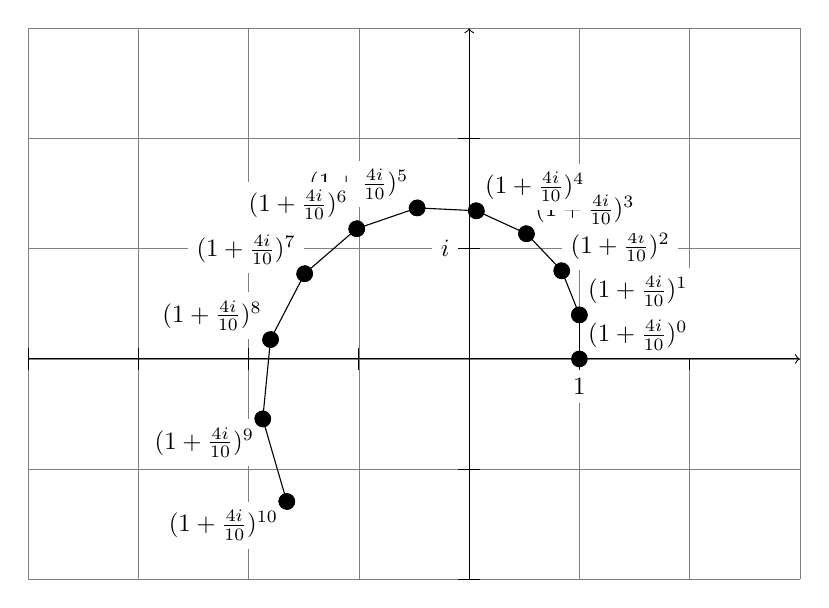
\begin{tikzpicture}[scale=1.4,every node/.style={scale=0.9}]
				    \draw[step=1,help lines] (-4.000000,-2.000000) grid (3.000000,3.000000);
            \draw[->] (-4.000000,0) -- (3.000000,0);
            \draw[->] (0,-2.000000) -- (0,3.000000);
            \draw (-4.000000, 0.100000) -- (-4.000000,-0.100000);
            \draw (-3.000000, 0.100000) -- (-3.000000,-0.100000);
            \draw (-2.000000, 0.100000) -- (-2.000000,-0.100000);
            \draw (-1.000000, 0.100000) -- (-1.000000,-0.100000);
            \draw (0.000000, 0.100000) -- (0.000000,-0.100000);
            \draw (1.000000, 0.100000) -- (1.000000,-0.100000);
            \draw (2.000000, 0.100000) -- (2.000000,-0.100000);
            \draw (0.100000, -2.000000) -- (-0.100000,-2.000000);
            \draw (0.100000, -1.000000) -- (-0.100000,-1.000000);
            \draw (0.100000, 0.000000) -- (-0.100000,0.000000);
            \draw (0.100000, 1.000000) -- (-0.100000,1.000000);
            \draw (0.100000, 2.000000) -- (-0.100000,2.000000);
            \draw (1,-0.100000) node[anchor=north,fill=white]{$1$};
            \draw (-0.100000,1) node[anchor=east,fill=white]{$i$};
            \draw (1.000000,0.000000) node[anchor=south west,fill=white]{$(1+\frac{4i}{10})^{0}$};
            \filldraw (1.000000,0.000000) circle (2pt);
            \draw (1.000000,0.000000) -- (1.000000,0.400000);
            \filldraw (1.000000,0.400000) circle (2pt);
            \draw (1.000000,0.400000) node[anchor=south west,fill=white]{$(1+\frac{4i}{10})^{1}$};
            \filldraw (1.000000,0.400000) circle (2pt);
            \draw (1.000000,0.400000) -- (0.840000,0.800000);
            \filldraw (0.840000,0.800000) circle (2pt);
            \draw (0.840000,0.800000) node[anchor=south west,fill=white]{$(1+\frac{4i}{10})^{2}$};
            \filldraw (0.840000,0.800000) circle (2pt);
            \draw (0.840000,0.800000) -- (0.520000,1.136000);
            \filldraw (0.520000,1.136000) circle (2pt);
            \draw (0.520000,1.136000) node[anchor=south west,fill=white]{$(1+\frac{4i}{10})^{3}$};
            \filldraw (0.520000,1.136000) circle (2pt);
            \draw (0.520000,1.136000) -- (0.065600,1.344000);
            \filldraw (0.065600,1.344000) circle (2pt);
            \draw (0.065600,1.344000) node[anchor=south west,fill=white]{$(1+\frac{4i}{10})^{4}$};
            \filldraw (0.065600,1.344000) circle (2pt);
            \draw (0.065600,1.344000) -- (-0.472000,1.370240);
            \filldraw (-0.472000,1.370240) circle (2pt);
            \draw (-0.472000,1.370240) node[anchor=south east,fill=white]{$(1+\frac{4i}{10})^{5}$};
            \filldraw (-0.472000,1.370240) circle (2pt);
            \draw (-0.472000,1.370240) -- (-1.020096,1.181440);
            \filldraw (-1.020096,1.181440) circle (2pt);
            \draw (-1.020096,1.181440) node[anchor=south east,fill=white]{$(1+\frac{4i}{10})^{6}$};
            \filldraw (-1.020096,1.181440) circle (2pt);
            \draw (-1.020096,1.181440) -- (-1.492672,0.773402);
            \filldraw (-1.492672,0.773402) circle (2pt);
            \draw (-1.492672,0.773402) node[anchor=south east,fill=white]{$(1+\frac{4i}{10})^{7}$};
            \filldraw (-1.492672,0.773402) circle (2pt);
            \draw (-1.492672,0.773402) -- (-1.802033,0.176333);
            \filldraw (-1.802033,0.176333) circle (2pt);
            \draw (-1.802033,0.176333) node[anchor=south east,fill=white]{$(1+\frac{4i}{10})^{8}$};
            \filldraw (-1.802033,0.176333) circle (2pt);
            \draw (-1.802033,0.176333) -- (-1.872566,-0.544480);
            \filldraw (-1.872566,-0.544480) circle (2pt);
            \draw (-1.872566,-0.544480) node[anchor=north east,fill=white]{$(1+\frac{4i}{10})^{9}$};
            \filldraw (-1.872566,-0.544480) circle (2pt);
            \draw (-1.872566,-0.544480) -- (-1.654774,-1.293507);
            \filldraw (-1.654774,-1.293507) circle (2pt);
            \draw (-1.654774,-1.293507) node[anchor=north east,fill=white]{$(1+\frac{4i}{10})^{10}$};
            \filldraw (-1.654774,-1.293507) circle (2pt);
			    \end{tikzpicture}
		    \end{minipage}
		    \begin{minipage}[c]{0.35\textwidth}
			    A plot of the list of complex numbers $(1+\frac{4i}{10})^{[0:11]}$. Notice that each multiplication of a complex number by $1+\frac{4i}{10}$ results in an anti-clockwise rotation about the origin and a small radial movement outwards. This can be seen to reflect the computation $(1+\frac{4i}{10})a=1a+\frac{4}{10}(ai)$ after one notes that $ai$ is perpendicular to $a$. Also note that each line segment has a length of roughly $\frac{4}{10}$ units. Hence the entire path has a length of approximately $10*\frac{4}{10}=4$ units.
		    \end{minipage}
	    \begin{multicols*}{2}
		    \declaration{3.17}
			    The notation \gls{complexcos}, where $z$ is a complex number and $n$ is a positive integer, will be used as a shorthand for $\frac{\exp_n(iz)+\exp_n(-iz)}{2}$.
		    \procedure{3.22}
			    \objective
				    Choose a rational number $x$ and a positive integer $n$. The objective of the following instructions is to show that $\Re(\exp_n(ix))=\cos_n(x)$.
			    \implementation
				    \begin{enumerate}
					    \item Verify that $\Re(\exp_n(ix))$
					    \begin{enumerate}
						    \item $=\frac{\exp_n(ix)+\conj{\exp_n(ix)}}{2}$
						    \item $=\frac{\exp_n(ix)+\exp_n(\conj{ix})}{2}$
						    \item $=\frac{\exp_n(ix)+\exp_n(-ix)}{2}$
						    \item $=\cos_n(x)$.
					    \end{enumerate}
				    \end{enumerate}
		    \declaration{3.18}
			    The notation \gls{complexsin}, where $z$ is a complex number and $n$ is a positive integer, will be used as a shorthand for $\frac{\exp_n(iz)-\exp_n(-iz)}{2i}$.
		    \procedure{3.23}
			    \objective
				    Choose a rational number $x$ and a positive integer $n$. The objective of the following instructions is to show that $\Im(\exp_n(ix))=\sin_n(x)$.
			    \implementation
				    \begin{enumerate}
					    \item Verify that $\Im(\exp_n(ix))$
					    \begin{enumerate}
						    \item $=\frac{\exp_n(ix)-\conj{\exp_n(ix)}}{2i}$
						    \item $=\frac{\exp_n(ix)-\exp_n(\conj{ix})}{2i}$
						    \item $=\frac{\exp_n(ix)-\exp_n(-ix)}{2i}$
						    \item $=\sin_n(x)$.
					    \end{enumerate}
				    \end{enumerate}
		    \procedure{3.24}
			    \objective
				    Choose a rational number $X\ge 0$. The objective of the following instructions is to construct two rational numbers $a,b$, and a procedure, $p(x,y,n)$, to show that $\cos_n(x+y)\equiv\cos_n(x)\cos_n(y)-\sin_n(x)\sin_n(y)\err{\frac{axy}{n}}\err{\frac{aX^2}{n}}$ when two complex numbers $x,y$ and a positive integer $n>b$ such that $\lVert x\rVert^2\le X^2$ and $\lVert y\rVert^2\le X^2$ are chosen.
			    \implementation
				    \begin{enumerate}
					    \item Execute \procedurehr{3.15} on $\langle X\rangle$ and let $\langle a,b,q\rangle$ receive.
					    \item Let $p(x,y,n)$ be the following procedure:
					    \begin{enumerate}
					      \item Using procedure $q$, verify that $\cos_n(x+y)$
					      \begin{enumerate}
					        \item $=\frac{1}{2}(\exp_n(i(x+y))+\exp_n(-i(x+y)))$
					        \item $\equiv\frac{1}{2}(\exp_n(ix)\exp_n(iy)+\exp_n(-i(x+y)))\err{\frac{a(ix)(iy)}{2n}}$
					        \item $\equiv\frac{1}{2}(\exp_n(ix)\exp_n(iy)+\exp_n(-ix)\exp_n(-iy))\allowbreak\err{\frac{a(-ix)(-iy)}{2n}}$
					        \item $=\frac{1}{4}(\exp_n(ix)\exp_n(iy)+\exp_n(-ix)\exp_n(-iy))+\frac{1}{4}(\exp_n(ix)\exp_n(iy)+\exp_n(-ix)\exp_n(-iy))$
					        \item $=\frac{1}{4}(\exp_n(ix)(\exp_n(iy)+\exp_n(-iy))+(\exp_n(-ix)-\exp_n(ix))\exp_n(-iy))+\frac{1}{4}((\exp_n(ix)-\exp_n(-ix))\exp_n(iy)+\exp_n(-ix)(\exp_n(iy)+\exp_n(-iy)))$
					        \item $=\frac{1}{2}\exp_n(ix)\cos_n(y)+\frac{1}{2i}\sin_n(x)\exp_n(-iy)-\frac{1}{2i}\sin_n(x)\exp_n(iy)+\frac{1}{2}\exp_n(-ix)\cos_n(y)$
					        \item $=\cos_n(x)\cos_n(y)-\sin_n(x)\sin_n(y)$
					      \end{enumerate}
					      \item \textbf{Hence verify that $\cos_n(x+y)\equiv\cos_n(x)\cos_n(y)-\sin_n(x)\sin_n(y)\err{\frac{axy}{n}}\err{\frac{aX^2}{n}}$.}
					    \end{enumerate}
					    \item \textbf{Yield the tuple $\langle a,b,p\rangle$.}
				    \end{enumerate}
		    \procedure{3.25}
			    \objective
				    Choose a rational number $X\ge 0$. The objective of the following instructions is to construct two rational numbers $a,b$, and a procedure, $p(x,y,n)$, to show that $\sin_n(x+y)\equiv\sin_n(x)\cos_n(y)-\cos_n(x)\sin_n(y)\err{\frac{axy}{n}}\err{\frac{aX^2}{n}}$ when two complex numbers $x,y$ and a positive integer $n>b$ such that $\lVert x\rVert^2\le X^2$ and $\lVert y\rVert^2\le X^2$ are chosen.
			    \implementation
				    Implementation is analogous to that of \procedurehr{3.24}.
		    \procedure{3.26}
			    \objective
				     Choose a rational number $X\ge 0$. The objective of the following instructions is to construct two rational numbers $a,b$, and a procedure, $p(x,n)$, to show that $\cos_n(x)^2+\sin_n(x)^2\equiv 1\err{\frac{a\lVert x\rVert^2}{n}}\err{\frac{aX^2}{n}}$ when a complex number $x$ and a positive integer $n$ such that $\lVert x\rVert^2\le X^2$ and $n>b$ are chosen.
			    \implementation
				    \begin{enumerate}
					    \item Execute \procedurehr{3.15} on $\langle X\rangle$ and let $\langle a,b,q\rangle$ receive.
					    \item Let $p(x,n)$ be the following procedure:
					    \begin{enumerate}
					      \item Using procedure $q$, verify that $\cos_n(x)^2+\sin_n(y)^2$
					      \begin{enumerate}
					        \item $=\frac{1}{4}(\exp_n(ix)+\exp_n(-ix))^2+\frac{1}{4i^2}(\exp_n(ix)-\exp_n(-ix))^2$
					        \item $=\frac{1}{4}(\exp_n(ix)^2+2\exp_n(ix)\exp_n(-ix)+\exp_n(-ix)^2-\exp_n(ix)^2+2\exp_n(ix)\exp_n(-ix)-\exp_n(-ix)^2)$
					        \item $=\exp_n(ix)\exp_n(-ix)$
					        \item $\equiv 1\err{\frac{a(-ix)(ix)}{n}}$.
					      \end{enumerate}
					      \item \textbf{Hence verify that $\cos_n(x)^2+\sin_n(y)^2\equiv 1\err{\frac{a\lVert x\rVert^2}{n}}\err{\frac{aX^2}{n}}$.}
					    \end{enumerate}
					    \item \textbf{Yield the tuple $\langle a,b,p\rangle$.}
				    \end{enumerate}
		    \procedure{sat0308190647}
		      \objective
		        Choose a rational number $X\ge 0$. The objective of the following instructions is to construct two rational numbers $a,b$, and a procedure, $p(x,y,n)$, to show that $\lVert x\exp_n(iy)\rVert^2\equiv\lVert x\rVert^2\err{\frac{a\lVert x\rVert^2\lVert y\rVert^2}{n}}\err{\frac{a\lVert x\rVert^2X^2}{n}}$ when a complex number $x$, a rational number $y$, and a positive integer $n$ such that $\lVert y\rVert^2\le X^2$ and $n>b$ are chosen.
		      \implementation
		        \begin{enumerate}
		          \item Execute \procedurehr{3.26} on $\langle X\rangle$ and let $\langle a,b,q\rangle$ receive.
		          \item Let $p(x,y,n)$ be the following procedure:
		          \begin{enumerate}
		            \item Using procedure $q$, \procedurehr{3.22}, and \procedurehr{3.23}, verify that $\lVert x\exp_n(iy)\rVert^2$
		            \begin{enumerate}
		              \item $=\lVert x\rVert^2\lVert\exp_n(iy)\rVert^2$
		              \item $=\lVert x\rVert^2\lVert\cos_n(y)+i\sin_n(y)\rVert^2$
		              \item $=\lVert x\rVert^2(\cos_n(y)^2+\sin_n(y)^2)$
		              \item $\equiv\lVert x\rVert^2\cdot 1\err{\lVert x\rVert^2\cdot\frac{a\lVert y\rVert^2}{n}}$.
		            \end{enumerate}
		            \item \textbf{Hence verify that $\lVert x\exp_n(iy)\rVert^2\equiv\lVert x\rVert^2\err{\frac{a\lVert xy\rVert^2}{n}}\err{\frac{a\lVert x\rVert^2X^2}{n}}$.}
		          \end{enumerate}
		        \end{enumerate}
		    \procedure{3.29}
			    \objective
				    Choose a rational number $X\ge 0$. The objective of the following instructions is to construct two rational numbers $a,N$, and a procedure, $p(x,n)$, to show that $\cos_n(x)\equiv\sum_r^{[0:\lceil\frac{n}{2}\rceil]}\frac{(-1)^rx^{2r}}{(2r)!}\err{\frac{a}{n}}$ when a complex number $x$ and an integer $n>N$ such that $\lVert x\rVert^2\le X^2$ is chosen.
			    \implementation
				    \begin{enumerate}
					    \item Execute \procedurehr{3.21} on $\langle X\rangle$ and let $\langle a,N,q\rangle$ receive.
					    \item Let $p(x,n)$ be the following procedure:
					    \begin{enumerate}
						    \item Using procedure $q$, verify that $\cos_n(x)$
						    \begin{enumerate}
						      \item $=\frac{\exp_n(ix)}{2}+\frac{\exp_n(-ix)}{2}$
						      \item $\equiv\frac{1}{2}\sum_r^{[0:{n+1}]}\frac{(ix)^{r}}{r!}+\frac{\exp_n(-ix)}{2}\err{\frac{a}{2n}}$
						      \item $\equiv\frac{1}{2}\sum_r^{[0:{n+1}]}\frac{(ix)^{r}}{r!}+\frac{1}{2}\sum_r^{[0:{n+1}]}\frac{(-ix)^{r}}{r!}\err{\frac{a}{2n}}$
						      \item $=\sum_r^{[0:{n+1}]}\frac{(i^r+(-i)^r)x^{r}}{2(r!)}$
						      \item $=\sum_r^{[0:{n+1}]}\frac{[r\bmod 2=0](-1)^{\frac{r}{2}}x^{r}}{r!}$
						      \item $=\sum_r^{[0:{\lceil\frac{n}{2}\rceil}]}\frac{(-1)^rx^{2r}}{(2r)!}$.
						    \end{enumerate}
						    \item \textbf{Hence verify that $\cos_n(x)\equiv\sum_r^{[0:{\lceil\frac{n}{2}\rceil}]}\frac{(-1)^rx^{2r}}{(2r)!}\err{\frac{a}{n}}$.}
					    \end{enumerate}
				    \end{enumerate}
		    \procedure{3.30}
			    \objective
				    Choose a rational number $X\ge 0$. The objective of the following instructions is to construct two rational numbers $a,N$, and a procedure, $p(x,n)$, to show that $\sin_n(x)\equiv\sum_r^{[0:\lfloor\frac{n+1}{2}\rfloor]}\frac{(-1)^rx^{2r+1}}{(2r+1)!}\err{\frac{a}{n}}$ when a complex number $x$ and an integer $n>N$ such that $\lVert x\rVert^2\le X^2$ is chosen.
			    \implementation
				    Implementation is analogous to that of \procedurehr{3.29}.
	    \end{multicols*}
	  \chapter{Binomial and Mercator Series}
	    \begin{multicols*}{2}
		    \declaration{sun2107190610}
			    The notation \gls{complexbinomialseries}, where $x,a$ are complex numbers and $n$ is a positive integer, will be used as a shorthand for $\sum_r^{[0:n]}\binom{a}{r}x^r$.
	      \procedure{sun2107190619}
	        \objective
	          Choose a complex number $x$ and two non-negative integers $a,n$ such that $n>a$. The objective of the following instructions is to show that $(1+x)_n^a=(1+x)^a$.
	        \implementation
	          \begin{enumerate}
	            \item Using \procedurehr{sun2107190636}, verify that $(1+x)^a_n=$
	            \begin{enumerate}
	              \item $=\sum_r^{[0:n]}\binom{a}{r}x^r$
	              \item $=\sum_r^{[0:n]}\frac{a^{\ul{r}}}{r!}x^r$
	              \item $=\sum_r^{[0:a+1]}\frac{a^{\ul{r}}}{r!}x^r+\sum_r^{[a+1:n]}\frac{a^{\ul{r}}}{r!}x^r$
	              \item $=\sum_r^{[0:a+1]}\frac{a^{\ul{r}}}{r!}x^r+\sum_r^{[a+1:n]}\frac{0}{r!}x^r$
	              \item $=\sum_r^{[0:a+1]}\binom{a}{r}x^r$
	              \item $=(1+x)^a$.
	            \end{enumerate}
	          \end{enumerate}
	      \procedure{sun2107190640}
	        \objective
	          Choose two complex numbers $x,y$ and a positive integer $N$. The objective of the following instructions is to show that $\binom{x+y}{N}=\sum_k^{N+1}\binom{x}{k}\binom{y}{N-k}$.
	        \implementation
	          \begin{enumerate}
	            \item If $N=0$, then do the following:
	            \begin{enumerate}
	              \item Verify that $\binom{x+y}{N}=1=\sum_k^{[0:N+1]}\binom{x}{k}\binom{y}{N-k}$.
	            \end{enumerate}
	            \item Otherwise do the following:
	            \begin{enumerate}
	              \item Verify that $N>0$.
	              \item Execute \procedurehr{sun2107190640} on $\langle x-1,y,N-1\rangle$.
	              \item Hence verify that $\binom{x+y-1}{N-1}=\sum_k^{[0:N]}\binom{x-1}{k}\binom{y}{N-1-k}$.
	              \item Execute \procedurehr{sun2107190640} on $\langle x,y-1,N-1\rangle$.
	              \item Hence verify that $\binom{x+y-1}{N-1}=\sum_k^{[0:N]}\binom{x}{k}\binom{y-1}{N-1-k}$.
	              \item Hence verify that $\binom{x+y}{N}$
	              \begin{enumerate}
	                \item $=\frac{x+y}{N}\binom{x+y-1}{N-1}$
	                \item $=\frac{x}{N}\binom{x+y-1}{N-1}+\frac{y}{N}\binom{x+y-1}{N-1}$
	                \item $=\frac{x}{N}\sum_k^{[0:N]}\binom{x-1}{k}\binom{y}{N-1-k}+\frac{y}{N}\sum_k^{[0:N]}\binom{x}{k}\binom{y-1}{N-1-k}$
	                \item $=\frac{x}{N}\sum_k^{[1:N+1]}\binom{x-1}{k-1}\binom{y}{N-k}+\frac{y}{N}\sum_k^{[0:N]}\binom{x}{k}\binom{y-1}{N-1-k}$
	                \item $=\sum_k^{[0:N+1]}\frac{k}{N}\binom{x}{k}\binom{y}{N-k}+\sum_k^{[0:N+1]}\frac{N-k}{N}\binom{x}{k}\binom{y}{N-k}$
	                \item $=\sum_k^{[0:N+1]}\binom{x}{k}\binom{y}{N-k}$.
	              \end{enumerate}
	            \end{enumerate}
	          \end{enumerate}
	      \procedure{sun2107191133}
	        \objective
	          Choose complex numbers $a,b,x$ and a natural number $n$. The objective of the following instructions is to show that $(1+x)_n^a(1+x)_n^b-(1+x)_n^{a+b}=\sum_k^{[1:n]}\sum_r^{[k:n]}\binom{a}{k+n-1-r}\binom{b}{r}x^{k+n-1}$.
	        \implementation
	          \begin{enumerate}
	            \item Verify that $(1+x)_n^a(1+x)_n^b-(1+x)_n^{a+b}$
	            \begin{enumerate}
	              \item $=(\sum_k^{[0:n]}\binom{a}{k}x^k)(\sum_r^{[0:n]}\binom{b}{r}x^r)-\sum_k^{[0:n]}\binom{a+b}{k}x^k$
	              \item $=\sum_k^{[0:n]}\sum_r^{[0:n]}\binom{a}{k}\binom{b}{r}x^{k+r}-\sum_k^{[0:n]}\binom{a+b}{k}x^k$
	              \item $=\sum_k^{[0:n]}\sum_r^{[0:k+1]}\binom{a}{k-r}\binom{b}{r}x^k+\sum_k^{[n:2n-1]}\sum_r^{[k-n+1:n]}\binom{a}{k-r}\binom{b}{r}x^k-\sum_k^{[0:n]}\binom{a+b}{k}x^k$
	              \item $=\sum_k^{[0:n]}\binom{a+b}{k}x^k+\sum_k^{[1:n]}\sum_r^{[k:n]}\binom{a}{k+n-1-r}\binom{b}{r}x^{k+n-1}-\sum_k^{[0:n]}\binom{a+b}{k}x^k$
	              \item $=\sum_k^{[1:n]}\sum_r^{[k:n]}\binom{a}{k+n-1-r}\binom{b}{r}x^{k+n-1}$.
	            \end{enumerate}
	          \end{enumerate}
	      \procedure{sun2107191247}
	        \objective
	          Choose two rational numbers $A>0$ and $0<X<1$. The objective of the following instructions is to construct rational numbers $Y>0$, $0<Z<1$ and a procedure $p(a,x,n)$ to show that $\lVert\binom{a}{n}x^n\rVert^2\le(YZ^n)^2$ when complex numbers $a,x$ such that $\lVert a+1\rVert^2<A^2$ and $\lVert x\rVert^2<X^2$ are chosen.
	        \implementation
	          \begin{enumerate}
	            \item Let $e=\frac{AX}{1-X}-1$.
	            \item Let $d=\lfloor\frac{AX}{1-X}\rfloor$.
	            \item Verify that $d>e>-1$.
	            \item Let $Z=(1+\frac{A}{d+1})X$.
	            \item Verify that $0<Z<(1+\frac{A}{e+1})X=1$.
	            \item Let $Y=Z^{-d}\prod_k^{[0:d]}\frac{(A+k+1)X}{k+1}=Z^{-d}\prod_k^{[0:d]}X(1+\frac{A}{k+1})$.
	            \item Let $p(a,x,n)$ be the following procedure:
	            \begin{enumerate}
	              \item Verify that $\Re(a+1)^2\le\lVert a+1\rVert^2\le A^2$.
	              \item Hence verify that $\lvert\Re(a+1)\rvert\le A$.
	              \item Hence verify that $\lVert\binom{a}{n}x^n\rVert^2$
	              \begin{enumerate}
	                \item $=\lVert\frac{a^{\ul{n}}}{n!}x^n\rVert^2$
	                \item $=\lVert\prod_k^{[0:n]}(\frac{a+1-(k+1)}{k+1}\cdot x)\rVert^2$
	                \item $=\prod_k^{[0:n]}\frac{\lVert(a+1)-(k+1)\rVert^2\lVert x\rVert^2}{(k+1)^2}$
	                \item $=\prod_k^{[0:n]}\frac{(\lVert a+1\rVert^2-2\Re(a+1)(k+1)+(k+1)^2)\lVert x\rVert^2}{(k+1)^2}$
	                \item $\le\prod_k^{[0:n]}\frac{(A^2+2A(k+1)+(k+1)^2)X^2}{(k+1)^2}$
	                \item $=(\prod_k^{[0:n]}\frac{(A+k+1)X}{k+1})^2$
	                \item $=(\prod_k^{[0:n]}X(1+\frac{A}{k+1}))^2$.
	              \end{enumerate}
	              \item If $n\le d$, then do the following:
	              \begin{enumerate}
	                \item Verify that $\lVert\binom{a}{n}x^n\rVert^2$
	                \begin{enumerate}
	                  \item $\le(\prod_k^{[0:n]}X(1+\frac{A}{k+1}))^2$
	                  \item $=(\prod_k^{[0:d]}X(1+\frac{A}{k+1}))^2(\prod_k^{[n:d]}X(1+\frac{A}{k+1}))^{-2}$
	                  \item $\le(\prod_k^{[0:d]}X(1+\frac{A}{k+1}))^2(X(1+\frac{A}{d+1}))^{-2(d-n)}$
	                  \item $=Y^2Z^{2n}$.
	                \end{enumerate}
	              \end{enumerate}
	              \item Otherwise do the following:
	              \begin{enumerate}
	                \item Verify that $\lVert\binom{a}{n}x^n\rVert^2$
	                \begin{enumerate}
	                  \item $\le(\prod_k^{[0:n]}X(1+\frac{A}{k+1}))^2$
	                  \item $=(\prod_k^{[0:d]}X(1+\frac{A}{k+1}))^2(\prod_k^{[d:n]}X(1+\frac{A}{k+1}))^2$
	                  \item $\le(\prod_k^{[0:d]}X(1+\frac{A}{k+1}))^2(X(1+\frac{A}{d+1}))^{2(n-d)}$
	                  \item $=Y^2Z^{2n}$.
	                \end{enumerate}
	              \end{enumerate}
	            \end{enumerate}
	            \item \textbf{Yield the tuple $\langle Y,Z,p\rangle$.}
	          \end{enumerate}
	      \procedure{wed2407191422}
	        \objective
	          Choose a rational number $0<X<1$ and a positive integer $k$. The objective of the following instructions is to construct rational numbers $Y>0$, $0<Z<1$ and a procedure $p(x,n)$ to show that $\lVert n^kx^n\rVert^2\le(YZ^n)^2$ when a complex number $x$ such that $\lVert x\rVert^2\le X^2$ is chosen.
	        \implementation
	          \begin{enumerate}
	            \item Let $e=\frac{k}{1-X}-1$.
	            \item Let $d=\lfloor\frac{k}{1-X}\rfloor$.
	            \item Verify that $d>e>k-1$.
	            \item Let $Z=(1+\frac{1}{d})^kX$.
	            \item Verify that $Z<(1+\frac{1}{e})^kX$.
	            \item Now using \procedurehr{wed2407191348}, verify that $0<Z<(1+\frac{1}{e})^kX\le\frac{1+\frac{1}{e}}{1-(k-1)\frac{1}{e}}\cdot X=1$.
	            \item Let $Y=Z^{-d}X\prod_r^{[1:d]}X(1+\frac{1}{r})^k$.
	            \item Let $p(x,n)$ be the following procedure:
	            \begin{enumerate}
	              \item Verify that $\lVert n^kx^n\rVert^2$
	              \begin{enumerate}
	                \item $\le\lVert x\prod_r^{[1:n]}x\cdot\frac{(r+1)^k}{r^k}\rVert^2$
	                \item $=\lVert x\rVert^2\prod_r^{[1:n]}\lVert x\rVert^2(\frac{(r+1)^k}{r^k})^2$
	                \item $\le X^2\prod_r^{[1:n]}((1+\frac{1}{r})^kX)^2$.
	              \end{enumerate}
	              \item If $n\le d$, then do the following:
	              \begin{enumerate}
	                \item Verify that $\lVert n^kx^n\rVert^2$
	                \begin{enumerate}
	                  \item $\le X^2(\prod_r^{[1:n]}X(1+\frac{1}{r})^k)^2$
	                  \item $=X^2(\prod_r^{[1:d]}X(1+\frac{1}{r})^k)^2\cdot(\prod_r^{[n:d]}X(1+\frac{1}{r})^k)^{-2}$
	                  \item $\le X^2(\prod_r^{[1:d]}X(1+\frac{1}{r})^k)^2(X(1+\frac{1}{d})^k)^{-2(d-n)}$
	                  \item $=Y^2Z^{2n}$.
	                \end{enumerate}
	              \end{enumerate}
	              \item Otherwise do the following:
	              \begin{enumerate}
	                \item Verify that $\lVert n^kx^n\rVert^2$
	                \begin{enumerate}
	                  \item $\le X^2(\prod_r^{[1:n]}X(1+\frac{1}{r})^k)^2$
	                  \item $=X^2(\prod_r^{[1:d]}X(1+\frac{1}{r})^k)^2(\prod_r^{[d:n]}X(1+\frac{1}{r})^k)^2$
	                  \item $\le X^2(\prod_r^{[1:d]}X(1+\frac{1}{r})^k)^2(X(1+\frac{1}{d})^k)^{2(n-d)}$
	                  \item $=Y^2Z^{2n}$.
	                \end{enumerate}
	              \end{enumerate}
	            \end{enumerate}
	            \item \textbf{Yield the tuple $\langle Y,Z,p\rangle$.}
	          \end{enumerate}
	      \procedure{wed2407191521}
	        \objective
	          Choose two rational numbers $A>0$, $1>X>0$. The objective of the following instructions is to construct rational numbers $D>0$, $0<G<1$, and a procedure $p(x,a,b,n)$ to show that $(1+x)_n^{a+b}\equiv(1+x)_n^a(1+x)_n^b\err{DG^n}$ when $\lVert x\rVert^2\le X$, and $\lVert a\rVert^2,\lVert b\rVert^2<A$.
	        \implementation
	          \begin{enumerate}
	            \item Execute \procedurehr{sun2107191247} on $\langle A,X\rangle$ and let $\langle B,C,q\rangle$ receive.
	            \item Execute \procedurehr{wed2407191422} on $\langle C,1\rangle$ and let $\langle F,G,t\rangle$ receive.
	            \item Let $D=\frac{B^2F}{1-C}$.
	            \item Let $p(x,a,b,n)$ be the following procedure:
	            \begin{enumerate}
	              \item For each $r\in[1:n]$, do the following:
	              \begin{enumerate}
	                \item Using procedure $q$, verify that $\lVert\binom{a}{r}x^r\rVert^2\le(BC^r)^2$.
	                \item Using procedure $q$, verify that $\lVert\binom{b}{r}x^r\rVert^2\le(BC^r)^2$.
	              \end{enumerate}
	              \item Using procedure $t$, verify that $\lVert nC^n\rVert^2\le(FG^n)^2$.
	              \item Hence verify that $(1+x)_n^{a+b}\equiv(1+x)_n^a(1+x)_n^b$
	              \begin{enumerate}
	                \item $\err{(1+x)_n^a(1+x)_n^b-(1+x)_n^{a+b}}$
	                \item $\err{\sum_k^{[1:n]}\sum_r^{[k:n]}\binom{a}{k+n-1-r}\binom{b}{r}x^{k+n-1}}$
	                \item $\err{\sum_k^{[1:n]}\sum_r^{[k:n]}\binom{a}{k+n-1-r}x^{k+n-1-r}\binom{b}{r}x^r}$
	                \item $\err{\sum_k^{[1:n]}\sum_r^{[k:n]}BC^{k+n-1-r}BC^r}$
	                \item $\err{B^2C^n\sum_k^{[1:n]}\sum_r^{[k:n]}C^{k-1}}$
	                \item $\err{B^2C^n\sum_r^{[1:n]}\sum_k^{[1:r+1]}C^{k-1}}$
	                \item $\err{B^2C^n\sum_r^{[1:n]}\frac{1}{1-C}}$
	                \item $\err{\frac{B^2}{1-C}\cdot nC^n}$
	                \item $\err{\frac{B^2F}{1-C}G^n}$
	                \item $\err{DG^n}$.
	              \end{enumerate}
	            \end{enumerate}
	          \end{enumerate}
	      \procedure{wed2407191611}
	        \objective
	          Choose two rational numbers $A>0$, $1>X>0$. The objective of the following instructions is to construct a rational number $D$ and a procedure $p(x,n,a,k)$ to show that $\lVert((1+x)_n^a)^k\rVert^2<D^2$ when complex numbers $x,a$ and positive integers $n,k$ such that $\lVert x\rVert^2<X^2$ and $\lVert ka\rVert^2<A^2$.
	        \implementation
	          \begin{enumerate}
	            \item Execute \procedurehr{3.13} on $\langle\frac{ABX}{1-C}\rangle$ and let $\langle E,N,t\rangle$ receive.
	            \item Execute \procedurehr{sun2107191247} on $\langle A+1,X\rangle$ and let $\langle B,C,q\rangle$ receive.
	            \item Let $D=\max(E,(1+\frac{ABX}{1-C})^{\lfloor N\rfloor})$.
	            \item Let $p(x,n,a,k)$ be the following procedure:
	            \begin{enumerate}
	              \item For each $r\in[1:n]$, do the following:
	              \begin{enumerate}
	                \item Verify that $\lVert a\rVert^2\le\lVert ka\rVert^2\le A^2$.
	                \item Verify that $\lVert a-1\rVert^2\le(A+1)^2$.
	                \item Execute procedure $q$ on $\langle a-1,x,r-1\rangle$.
	                \item Hence verify that $\lVert\binom{a-1}{r-1}x^{r-1}\rVert^2\le(BC^r)^2$.
	              \end{enumerate}
	              \item Hence verify that $\lVert k\sum_r^{[1:n]}\binom{a}{r}x^r\rVert^2$
	              \begin{enumerate}
	                \item $=\lVert k\sum_r^{[1:n]}\frac{a}{r}\binom{a-1}{r-1}x^r\rVert^2$
	                \item $=\lVert kax\sum_r^{[1:n]}\frac{1}{r}\binom{a-1}{r-1}x^{r-1}\rVert^2$
	                \item $\le(AX\sum_r^{[1:n]}BC^{r-1})^2$
	                \item $\le(\frac{ABX}{1-C})^2$.
	              \end{enumerate}
	              \item If $k>N$, then do the following:
	              \begin{enumerate}
	                \item Execute procedure $t$ on $\langle k\sum_r^{[1:n]}\binom{a}{r}x^r\rangle$.
	                \item Hence verify that $\lVert((1+x)_n^a)^k\rVert^2$
	                \begin{enumerate}
	                  \item $=\lVert(\sum_r^{[0:n]}\binom{a}{r}x^r)^k\rVert^2$
	                  \item $=\lVert(1+\sum_r^{[1:n]}\binom{a}{r}x^r)^k\rVert^2$
	                  \item $=\lVert\exp_k(k\sum_r^{[1:n]}\binom{a}{r}x^r)\rVert^2$
	                  \item $\le E^2$
	                  \item $\le D^2$.
	                \end{enumerate}
	              \end{enumerate}
	              \item Otherwise do the following:
	              \begin{enumerate}
	                \item Verify that $\lVert\sum_r^{[1:n]}\binom{a}{r}x^r)^k\rVert^2$
	                \begin{enumerate}
	                  \item $\le\lVert k\sum_r^{[1:n]}\binom{a}{r}x^r\rVert^2$
	                  \item $\le(\frac{ABX}{1-C})^2$.
	                \end{enumerate}
	                \item Hence verify that $\lVert((1+x)_n^a)^k\rVert^2$
	                \begin{enumerate}
	                  \item $=(\lVert(1+x)_n^a\rVert^2)^k$
	                  \item $=(\lVert 1+\sum_r^{[1:n]}\binom{a}{r}x^r\rVert^2)^k$
	                  \item $\le(1+\frac{ABX}{1-C})^{2k}$
	                  \item $\le D^2$.
	                \end{enumerate}
	              \end{enumerate}
	            \end{enumerate}
	            \item \textbf{Yield $\langle D,p\rangle$.}
	          \end{enumerate}
	      \procedure{tue2008190712}
	        \objective
	          Choose two rational numbers $A>0$, $1>X>0$. The objective of the following instructions is to construct positive rational numbers $D,N$, and a procedure $p(x,a,n)$ to show that $\lVert(1+x)_n^a\rVert^2\ge D^2$ when complex numbers $x,a$ and an integer $n$ such that $\lVert x\rVert^2\le X^2$, $\lVert a\rVert\le A^2$, and $n>N$ are chosen.
	        \implementation
	          \begin{enumerate}
	            \item Execute \procedurehr{wed2407191521} on $\langle A,X\rangle$ and let $\langle a_1,b_1,p_1\rangle$ receive.
	            \item Execute \procedurehr{wed2407191422} on $\langle b_1,1\rangle$ and let $\langle a_2,b_2,p_2\rangle$ receive.
	            \item Execute \procedurehr{wed2407191611} on $\langle A,X\rangle$ and let $\langle a_3,p_3\rangle$ receive.
	            \item Let $D=\frac{1}{2a_3}$.
	            \item Let $N=2a_1a_2$.
	            \item Let $p(x,a,n)$ be the following procedure:
	            \begin{enumerate}
	              \item Using procedure $p_2$, verify that $\lVert n{b_1}^n\rVert^2\le(a_2{b_2}^n)^2\le{a_2}^2$.
	              \item Hence verify that $(a_1{b_1}^n)^2\le(\frac{a_1a_2}{n})^2$.
	              \item Using procedure $p_3$, verify that $\lVert((1+x)_n^{-a})^1\rVert^2\le{a_3}^2$.
	              \item Using procedure $p_1$, verify that $\lVert(1+x)_n^{-a}(1+x)_n^a-1\rVert^2$
	              \begin{enumerate}
	                \item $=\lVert(1+x)_n^{-a}(1+x)_n^a-(1+x)_n^{-a+a}\rVert^2$
	                \item $\le(a_1{b_1}^n)^2$.
	              \end{enumerate}
	              \item Hence using \procedurehr{3.05}, verify that $\frac{1}{2}-\lVert(1+x)_n^{-a}(1+x)_n^a\rVert^2$
	              \begin{enumerate}
	                \item $=\frac{1}{2}\lVert 1\rVert^2-\lVert(1+x)_n^{-a}(1+x)_n^a\rVert^2$
	                \item $\le\lVert 1-(1+x)_n^{-a}(1+x)_n^a\rVert^2$
	                \item $\le(a_1{b_1}^n)^2$
	                \item $\le(\frac{a_1a_2}{n})^2$
	                \item $\le\frac{1}{4}$.
	              \end{enumerate}
	              \item Hence verify that $(\frac{1}{2})^2$
	              \begin{enumerate}
	                \item $\le\lVert(1+x)_n^{-a}(1+x)_n^a\rVert^2$
	                \item $\le{a_3}^2\lVert(1+x)_n^a\rVert^2$.
	              \end{enumerate}
	              \item \textbf{Hence verify that $D^2\le\lVert(1+x)_n^a\rVert^2$.}
	            \end{enumerate}
	            \item \textbf{Yield the tuple $\langle D,N,p\rangle$.}
	          \end{enumerate}
	      \procedure{tue2008190849}
	        \objective
	          Choose two rational numbers $A>0$ and $1>X>0$. The objective of the following instructions is to construct positive rational numbers $B,C,D$, and a procedure $p(x,a,b,n)$ to show that $(1+x)_n^{a-b}\equiv\frac{(1+x)_n^a}{(1+x)_n^b}\err{BC^n}$ when complex numbers $x,a,b$ and an integer $n$ such that $\lVert x\rVert^2\le X^2$, $\lVert a\rVert^2\le A^2$, $\lVert b\rVert^2\le A^2$, and $n>D$ are chosen.
	        \implementation
	          \begin{enumerate}
	            \item Execute \procedurehr{wed2407191521} on $\langle A,X\rangle$ and let $\langle a_1,C,p_1\rangle$ receive.
	            \item Execute \procedurehr{tue2008190712} on $\langle A,X\rangle$ and let $\langle a_2,D,p_2\rangle$ receive.
	            \item Execute \procedurehr{wed2407191611} on $\langle A,X\rangle$ and let $\langle a_3,p_3\rangle$ receive.
	            \item Let $B=(1+\frac{a_3}{a_2})a_1$.
	            \item Let $p(x,a,b,n)$ be the following procedure:
	            \begin{enumerate}
	              \item Using procedures $p_1,p_2,p_3$, verify that $(1+x)_n^{a-b}$
	              \begin{enumerate}
	                \item $\equiv(1+x)_n^a(1+x)_n^{-b}\err{a_1{C}^n}$
	                \item $=(1+x)_n^a\frac{(1+x)_n^{b}(1+x)_n^{-b}}{(1+x)_n^{b}}$
	                \item $\equiv((1+x)_n^a)^1\frac{(1+x)_n^{b-b}}{(1+x)_n^{b}}\err{a_3\frac{a_1{C}^n}{a_2}}$
	                \item $=\frac{(1+x)_n^a}{(1+x)_n^b}$
	              \end{enumerate}
	              \item \textbf{Hence verify that $(1+x)_n^{a-b}\equiv\frac{(1+x)_n^a}{(1+x)_n^b}\err{(1+\frac{a_3}{a_2})a_1{C}^n}\err{BC^n}$.}
	            \end{enumerate}
	            \item \textbf{Yield the tuple $\langle B,C,D,p\rangle$.}
	          \end{enumerate}
	      \procedure{wed2407191627}
	        \objective
	          Choose two rational numbers $A>0$, $1>X>0$. The objective of the following instructions is to construct rational numbers $G>0$, $0<C<1$, and a procedure $p(x,n,a,k)$ to show that $(1+x)_n^{ka}\equiv((1+x)_n^a)^k\err{GkC^n}$ when a non-negative integer $k$ and complex numbers $x,a$ such that $\lVert x\rVert^2\le X^2$ and $\lVert ka\rVert^2<A^2$ are chosen.
	        \implementation
	          \begin{enumerate}
	            \item Execute \procedurehr{wed2407191611} on $\langle A,X\rangle$ and let $\langle D,t\rangle$ receive.
	            \item Execute \procedurehr{wed2407191521} on $\langle A,X\rangle$ and let $\langle B,C,q\rangle$ receive.
	            \item Let $G=DB$.
	            \item Let $p(x,n,a,k)$ be the following procedure:
	            \begin{enumerate}
	              \item Hence using procedures $t,q$, verify that $(1+x)_n^{ka}$
	              \begin{enumerate}
	                \item $=((1+x)_n^a)^0(1+x)_n^{ka}$
	                \item $\equiv((1+x)_n^a)^1(1+x)_n^{(k-1)a}\err{DBC^n}$
	                \item $\equiv((1+x)_n^a)^2(1+x)_n^{(k-2)a}\err{DBC^n}$
	                \item $\vdots$
	                \item $\equiv((1+x)_n^a)^k(1+x)_n^{(k-k)a}\err{DBC^n}$
	                \item $=((1+x)_n^a)^k$.
	              \end{enumerate}
	              \item \textbf{Hence verify that $(1+x)_n^{ka}\equiv((1+x)_n^a)^k\err{kDBC^n}\err{GkC^n}$.}
	            \end{enumerate}
	            \item \textbf{Yield the tuple $\langle G,C,D,p\rangle$.}
	          \end{enumerate}
	      \procedure{sun0812190858}
	        \objective
	          Choose two non-negative rational numbers $a,b$ and two non-negative integers $r,n$ such that $b<r<n-a-1$. The objective of the following instructions is to show that $\sgn(\binom{b}{r}\binom{a}{n-r})=\sgn(\binom{b}{r+1}\binom{a}{n-r-1})$.
	        \implementation
	          \begin{enumerate}
	            \item Verify that $r>b$ and $n-r>a+1$.
	            \item Hence verify that $\frac{b-r}{(a+1)-(n-r)}>0$.
	            \item Hence verify that $\frac{b-r}{r+1}\cdot\frac{n-r}{a-n+r+1}>0$.
	            \item Hence verify that $\sgn(\frac{b-r}{r+1}\cdot\frac{n-r}{a-n+r+1})=1$.
	            \item Hence verify that $\sgn(\binom{b}{r+1}\binom{a}{n-r-1})$
	            \begin{enumerate}
	              \item $=\sgn(\frac{b-r}{r+1}\binom{b}{r}\cdot\frac{n-r}{a-n+r+1}\binom{a}{n-r})$
	              \item $=\sgn(\frac{b-r}{r+1}\cdot\frac{n-r}{a-n+r+1})\sgn(\binom{b}{r}\binom{a}{n-r})$
	              \item $=\sgn(\binom{b}{r}\binom{a}{n-r})$.
	            \end{enumerate}
	          \end{enumerate}
	      \procedure{sun0812190920}
	        \objective
	          Choose two non-negative rational numbers $a,b$ and an integer $n\ge\lceil a\rceil+\lceil b\rceil$. The objective of the following instructions is to show that $\sum_r^{[0:n+1]}\lVert\binom{b}{r}\binom{a}{n-r}\rVert=\sum_r^{[0:\lceil b\rceil]}\lVert\binom{b}{r}\binom{a}{n-r}\rVert+\lVert\sum_r^{[\lceil b\rceil:\lceil n-a\rceil]}\binom{b}{r}\binom{a}{n-r}\rVert+\sum_r^{[\lceil n-a\rceil:n+1]}\lVert\binom{b}{r}\binom{a}{n-r}\rVert$.
	        \implementation
	          \begin{enumerate}
	            \item Verify that $\lceil b\rceil\le\lfloor n-a\rfloor$.
	            \item For $r$ in $[\lceil b\rceil:\lfloor n-a\rceil]$, do the following:
	            \begin{enumerate}
	              \item Execute \procedurehr{sun0812190858} on $\langle a,b,r,n\rangle$.
	              \item Hence verify that $\sgn(\binom{b}{r}\binom{a}{n-r})=\sgn(\binom{b}{r+1}\binom{a}{n-r-1})$.
	            \end{enumerate}
	            \item Hence verify that $\sum_r^{[\lceil b\rceil:\lceil n-a\rceil]}\lVert\binom{b}{r}\binom{a}{n-r}\rVert=\lVert\sum_r^{[\lceil b\rceil:\lceil n-a\rceil]}\binom{b}{r}\binom{a}{n-r}\rVert$.
	            \item Hence verify that $\sum_r^{[0:n+1]}\Vert\binom{b}{r}\binom{a}{n-r}\rVert$
	            \begin{enumerate}
	              \item $=\sum_r^{[0:\lceil b\rceil]}\Vert\binom{b}{r}\binom{a}{n-r}\rVert+\sum_r^{[\lceil b\rceil:\lceil n-a\rceil]}\Vert\binom{b}{r}\binom{a}{n-r}\rVert+\sum_r^{[\lceil n-a\rceil:n+1]}\Vert\binom{b}{r}\binom{a}{n-r}\rVert$
	              \item $=\sum_r^{[0:\lceil b\rceil]}\Vert\binom{b}{r}\binom{a}{n-r}\rVert+\lVert\sum_r^{[\lceil b\rceil:\lceil n-a\rceil]}\binom{b}{r}\binom{a}{n-r}\rVert+\sum_r^{[\lceil n-a\rceil:n+1]}\Vert\binom{b}{r}\binom{a}{n-r}\rVert$.
	            \end{enumerate}
	          \end{enumerate}
	      \procedure{wed2407191824}
	        \objective
	          Choose a rational number $A>0$. The objective of the following instructions is to construct rational numbers $M>1$, $N>0$, and a procedure $p(a,n)$ to show that $\lVert\binom{a}{n}\rVert^2\le(\frac{M}{n})^{2(\lceil a\rceil)}$ and $\frac{M}{n}<1$ when a rational number $-1<a<A$ and an integer $n>N$ are chosen.
	        \implementation
	          \begin{enumerate}
	            \item Let $M=2A$.
	            \item Let $N=2A$.
	            \item Let $p(a,n)$ be the following procedure:
	            \begin{enumerate}
	              \item Verify that $-1<a<A$.
	              \item Verify that $n>N=2A>2a$.
	              \item Hence verify that $\frac{2a}{n}<\frac{2A}{2A}=1$.
	              \item Verify that $\frac{n}{2}>a$.
	              \item Therefore verify that $n-\lfloor a\rfloor>n-a>n-\frac{n}{2}=\frac{n}{2}$.
	              \item Hence verify that $\lVert\binom{a}{n}\rVert^2$
	              \begin{enumerate}
	                \item $=\lVert\frac{a^{\ul{n}}}{n!}\rVert^2$
	                \item $=\lVert\prod_k^{[0:n]}\frac{a-k}{k+1}\rVert^2$
	                \item $=\prod_k^{[0:n]}\frac{(a-k)^2}{(k+1)^2}$
	                \item $=\prod_k^{[0:\lceil a\rceil]}(k-a)^2\cdot\prod_k^{[0:n]}\frac{(k+\lfloor a\rfloor+1-a)^2}{(k+1)^2}\cdot\prod_k^{[n-\lceil a\rceil:n]}\frac{1}{(k+1)^2}$
	                \item $\le(a^{\lceil a\rceil}\cdot 1^n\cdot(\frac{1}{n-\lfloor a\rfloor})^{\lceil a\rceil})^2$
	                \item $=(\frac{a}{n-\lfloor a\rfloor})^{2(\lceil a\rceil)}$
	                \item $\le(\frac{2a}{n})^{2(\lceil a\rceil)}$
	                \item $\le(\frac{M}{n})^{2(\lceil a\rceil)}$.
	              \end{enumerate}
	            \end{enumerate}
	            \item \textbf{Yield the tuple $\langle M,N,p\rangle$.}
	          \end{enumerate}
	      \procedure{sun0812191002}
	        \objective
	          Choose a positive integer $A$. The objective of the following instructions is to construct a rational number $B$, an integer $N$, and a procedure $p(a,b,n)$ to show that $\sum_r^{[0:n+1]}\lVert\binom{b}{r}\binom{a}{n-r}\rVert\le\frac{B}{n}$ when non-negative rational numbers $a,b$, and an integer $n$ such that $a<A$,$b<A$, and $n>N$ are chosen.
	        \implementation
	          \begin{enumerate}
	            \item Execute \procedurehr{wed2407191824} on $\langle A\rangle$ and let $\langle M,Q,q\rangle$ receive.
	            \item Let $N=\max(2A,Q+A)$.
	            \item Let $B=M^A(M^{A}+8A!A)$.
	            \item Let $p(a,b,n)$ be the following procedure:
	            \begin{enumerate}
	              \item Verify that $n>N\ge Q$.
	              \item Execute procedure $q$ on $\langle a+b,n\rangle$.
	              \item Hence verify that $\lVert\binom{a+b}{n}\rVert\le(\frac{M}{n})^{\lceil a+b\rceil}\le\frac{M^{\lceil A+b\rceil}}{n}\le\frac{M^{A+\lceil b\rceil}}{n}\le\frac{M^{2A}}{n}$.
	              \item For $r$ in $[0:\lceil b\rceil]$, do the following:
	              \begin{enumerate}
	                \item Verify that $n-r\ge N-\lceil b\rceil\ge Q+A-A=Q$.
	                \item Execute procedure $q$ on $\langle a,n-r\rangle$.
	                \item Hence verify that $\lVert\binom{a}{n-r}\rVert^2\le(\frac{M}{n-r})^{2\lceil a\rceil}\le(\frac{M^A}{r})^2\le(\frac{M^A}{n-\lfloor a\rfloor})^2\le(\frac{M^A}{n-A})^2\le(\frac{M^A}{n-\frac{1}{2}N})^2\le(\frac{M^A}{\frac{1}{2}n})^2=(\frac{2M^A}{n})^2$.
	              \end{enumerate}
	              \item For $r$ in $[\lceil n-a\rceil:n+1]$, do the following:
	              \begin{enumerate}
	                \item Verify that $r\ge\lceil n-a\rceil=n-\lfloor a\rfloor\ge N-\lfloor a\rfloor\ge Q+A-A=Q$.
	                \item Execute procedure $q$ on $\langle b,r\rangle$.
	                \item Hence verify that $\lVert\binom{b}{r}\rVert^2\le(\frac{M}{r})^{2\lceil b\rceil}\le(\frac{M^A}{r})^2\le(\frac{2M^A}{n})^2$.
	              \end{enumerate}
	              \item Hence using \procedurehr{sun0812190920}, verify that $\sum_r^{[0:n+1]}\lVert\binom{b}{r}\binom{a}{n-r}\rVert$
	              \begin{enumerate}
	                \item $=\sum_r^{[0:\lceil b\rceil]}\lVert\binom{b}{r}\binom{a}{n-r}\rVert+\lVert\sum_r^{[\lceil b\rceil:\lceil n-a\rceil]}\binom{b}{r}\binom{a}{n-r}\rVert+\sum_r^{[\lceil n-a\rceil:n+1]}\lVert\binom{b}{r}\binom{a}{n-r}\rVert$
	                \item $=\sum_r^{[0:\lceil b\rceil]}\lVert\binom{b}{r}\binom{a}{n-r}\rVert+\lVert\sum_r^{[0:n+1]}\binom{b}{r}\binom{a}{n-r}-\sum_r^{[0:\lceil b\rceil]}\binom{b}{r}\binom{a}{n-r}-\sum_r^{[\lceil n-a\rceil:n+1]}\binom{b}{r}\binom{a}{n-r}\rVert+\sum_r^{[\lceil n-a\rceil:n+1]}\lVert\binom{b}{r}\binom{a}{n-r}\rVert$
	                \item $=2\sum_r^{[0:\lceil b\rceil]}\lVert\binom{b}{r}\binom{a}{n-r}\rVert+\lVert\sum_r^{[0:n+1]}\binom{b}{r}\binom{a}{n-r}\rVert+2\sum_r^{[\lceil n-a\rceil:n+1]}\lVert\binom{b}{r}\binom{a}{n-r}\rVert$
	                \item $=\lVert\binom{a+b}{n}\rVert+2(\sum_r^{[0:\lceil b\rceil]}\lVert\binom{b}{r}\binom{a}{n-r}\rVert+\sum_r^{[\lceil n-a\rceil:n+1]}\lVert\binom{b}{r}\binom{a}{n-r}\rVert)$
	                \item $\le\frac{M^{2A}}{n}+2(\sum_r^{[0:\lceil b\rceil]}A!\frac{2M^A}{n}+\sum_r^{[\lceil n-a\rceil:n+1]}\frac{2M^A}{n}A!)$
	                \item $\le\frac{M^A}{n}(M^A+8\frac{A!A}{n})$
	                \item $=\frac{B}{n}$.
	              \end{enumerate}
	            \end{enumerate}
	            \item \textbf{Yield the tuple $\langle B,N,p\rangle$.}
	          \end{enumerate}
	      \procedure{thu2507190646}
	        \objective
	          Choose a rational number $1>X\ge 0$. The objective of the following instructions is to construct rational numbers $B>0$, $N>0$, and a procedure $p(x,a,b,n)$ to show that $(1+x)_n^{a+b}\equiv(1+x)_n^a(1+x)_n^b\err{\frac{B}{n}}$ when a complex number $x$, two positive rational numbers $a,b$, and a positive integer $n$ such that $\lVert x\rVert^2\le 1$, $\Re(x)\ge-X$, $a<1$, $b<1$, and $n>N$ are chosen.
	        \implementation
	          \begin{enumerate}
	            \item Execute \procedurehr{sun0812191002} on $\langle 1\rangle$ and let $\langle M,N,q\rangle$ receive.
	            \item Let $B=\frac{2M}{1-X}$.
	            \item Let $p(x,a,b,n)$ be the following procedure:
	            \begin{enumerate}
	              \item For $r\in[1:n]$, for $k\in[0:r]$, verify that $\binom{a}{k+1+n-r}(-1)^{k+1}-\binom{a}{k+n-r}(-1)^k$
	              \begin{enumerate}
	                \item $=(-1)^{k+1}(\binom{a}{k+1+n-r}+\binom{a}{k+n-r})$
	                \item $=(-1)^{k+1}\binom{a+1}{k+1+n-r}$
	                \item $=(-1)^{-(k+1)}\lVert\binom{a+1}{k+1+n-r}\rVert(-1)^{k+1+n-r}$
	                \item $=\lVert\binom{a+1}{k+1+n-r}\rVert(-1)^{n-r}$.
	              \end{enumerate}
	              \item Execute procedure $q$ on $\langle a,b,n\rangle$.
	              \item Hence verify that $\sum_r^{[0:n+1]}\lVert\binom{b}{r}\binom{a}{n-r}\rVert\le\frac{M}{n}$.
	              \item Verify that $\lVert x+1\rVert^2=\Re(x+1)^2+\Im(x)^2\ge(1-X)^2$.
	              \item Hence using \procedurehr{sun2107191133}, verify that $(1+x)_n^{a+b}\equiv(1+x)_n^a(1+x)_n^b$
	              \begin{enumerate}
	                \item $\err{(1+x)_n^a(1+x)_n^b-(1+x)_n^{a+b}}$
	                \item $\err{\sum_k^{[1:n]}\sum_r^{[k:n]}\binom{a}{k+n-1-r}\binom{b}{r}x^{k+n-1}}$
	                \item $\err{x^n\sum_r^{[1:n]}\binom{b}{r}\sum_k^{[0:r]}\binom{a}{k+n-r}x^k}$
	                \item $\err{x^n\sum_r^{[1:n]}\binom{b}{r}\sum_k^{[0:r]}(\binom{a}{k+1+n-r}(-1)^{k+1}\cdot\frac{(-x)^{k+1}}{-x-1}-\binom{a}{k+n-r}(-1)^k\cdot\frac{(-x)^k}{-x-1}-\frac{(-x)^{k+1}}{-x-1}(\binom{a}{k+1+n-r}(-1)^{k+1}-\binom{a}{k+n-r}(-1)^k))}$
	                \item $\err{\frac{x^n}{x+1}\sum_r^{[1:n]}\binom{b}{r}(\binom{a}{n}x^r-\binom{a}{n-r}-\sum_k^{[0:r]}(-x)^{k+1}(\binom{a}{k+1+n-r}(-1)^{k+1}-\binom{a}{k+n-r}(-1)^k))}$
	                \item $\err{\frac{1}{1-X}\sum_r^{[1:n]}\lVert\binom{b}{r}\rVert(\lVert\binom{a}{n}\rVert+\lVert\binom{a}{n-r}\rVert+\sum_k^{[0:r]}\lVert\binom{a}{k+1+n-r}(-1)^{k+1}-\binom{a}{k+n-r}(-1)^k\rVert)}$
	                \item $\err{\frac{1}{1-X}\sum_r^{[1:n]}\lVert\binom{b}{r}\rVert(\lVert\binom{a}{n}\rVert+\lVert\binom{a}{n-r}\rVert+\lVert\sum_k^{[0:r]}(\binom{a}{k+1+n-r}(-1)^{k+1}-\binom{a}{k+n-r}(-1)^k)\rVert)}$
	                \item $\err{\frac{1}{1-X}\sum_r^{[1:n]}\lVert\binom{b}{r}\rVert(\lVert\binom{a}{n}\rVert+\lVert\binom{a}{n-r}\rVert+\lVert\binom{a}{n}(-1)^r-\binom{a}{n-r}\rVert)}$
	                \item $\err{\frac{2}{1-X}\sum_r^{[1:n]}\lVert\binom{b}{r}\rVert\lVert\binom{a}{n-r}\rVert}$
	                \item $\err{\frac{B}{n}}$.
	              \end{enumerate}
	            \end{enumerate}
	            \item \textbf{Yield the tuple $\langle B,N,p\rangle$.}
	          \end{enumerate}
	      \procedure{thu2507191017}
	        \objective
	          Choose a rational number $0\le X<1$. The objective of the following instructions is to construct a positive rational number $D$ such that $D>1$, and a procedure $p(x,n,a,k)$ to show that $\lVert((1+x)_n^a)^k\rVert^2<D^2$ when a complex number $x$, a rational number $a$, and positive integers $n,k$ such that $\lVert x\rVert^2\le 1$, $\Re(x)\ge-X$, and $(ka)^2<1$ are chosen.
	        \implementation
	          \begin{enumerate}
	            \item Execute \procedurehr{3.13} on $\langle\frac{2}{1-X}\rangle$ and let $\langle E,N,q\rangle$ receive.
	            \item Let $D=\max(E,(1+\frac{2}{1-X})^{\lfloor N\rfloor})$.
	            \item Let $p(x,n,a,k)$ be the following procedure:
	            \begin{enumerate}
	              \item For $t\in[1:n]$, verify that $\binom{a}{t+1}(-1)^{t+1}-\binom{a}{t}(-1)^t$
	              \begin{enumerate}
	                \item $=(-1)^{t+1}(\binom{a}{t+1}+\binom{a}{t})$
	                \item $=(-1)^{t+1}\cdot\frac{(a+1)^{\ul{t+1}}}{(t+1)!}$
	                \item $>0$.
	              \end{enumerate}
	              \item Hence verify that $\lVert k\sum_t^{[1:n]}\binom{a}{t}x^t\rVert^2$
	              \begin{enumerate}
	                \item $=\lVert k\sum_t^{[1:n]}(\binom{a}{t+1}(-1)^{t+1}\cdot\frac{(-x)^{t+1}}{-x-1}-\binom{a}{t}(-1)^t\cdot\frac{(-x)^t}{-x-1}-\frac{(-x)^{t+1}}{-x-1}(\binom{a}{t+1}(-1)^{t+1}-\binom{a}{t}(-1)^t))\rVert^2$
	                \item $=\frac{k^2}{\lVert x+1\rVert^2}\lVert\binom{a}{n}x^n-\binom{a}{1}x^1-\sum_t^{[1:n]}(-x)^{t+1}(\binom{a}{t+1}(-1)^{t+1}-\binom{a}{t}(-1)^t)\rVert^2$
	                \item $\le\frac{k^2}{(\Re(x)+1)^2+\Im(x)^2}(\lvert\binom{a}{n}\rvert+a+\sum_t^{[1:n]}\lvert\binom{a}{t+1}(-1)^{t+1}-\binom{a}{t}(-1)^t\rvert)^2$
	                \item $\le\frac{k^2}{(1-X)^2}(\lvert\binom{a}{n}\rvert+a+\sum_t^{[1:n]}(\binom{a}{t+1}(-1)^{t+1}-\binom{a}{t}(-1)^t))^2$
	                \item $=\frac{k^2}{(1-X)^2}(\lvert\binom{a}{n}\rvert+a+\binom{a}{n}(-1)^n-\binom{a}{1}(-1)^1)^2$
	                \item $=\frac{k^2}{(1-X)^2}(\lvert\binom{a}{n}\rvert+a-\lvert\binom{a}{n}\rvert+a)^2$
	                \item $=(\frac{2ak}{1-X})^2$
	                \item $\le(\frac{2}{1-X})^2$.
	              \end{enumerate}
	              \item If $k>N$, then do the following:
	              \begin{enumerate}
	                \item Execute procedure $q$ on $\langle k\sum_t^{[1:n]}\binom{a}{t}x^t,k\rangle$.
	                \item Hence verify that $\lVert((1+x)_n^a)^k\rVert^2$
	                \begin{enumerate}
	                  \item $=\lVert(\sum_t^{[0:n]}\binom{a}{t}x^t)^k\rVert^2$
	                  \item $=\lVert(1+\sum_t^{[1:n]}\binom{a}{t}x^t)^k\rVert^2$
	                  \item $=\lVert\exp_k(k\sum_t^{[1:n]}\binom{a}{t}x^t)\rVert^2$
	                  \item $\le E^2$.
	                  \item $\le D^2$.
	                \end{enumerate}
	              \end{enumerate}
	              \item Otherwise do the following:
	              \begin{enumerate}
	                \item Verify that $\lVert\sum_t^{[1:n]}\binom{a}{t}x^t\rVert^2$
	                \begin{enumerate}
	                  \item $\le\lVert k\sum_t^{[1:n]}\binom{a}{t}x^t\rVert^2$
	                  \item $\le(\frac{2}{1-X})^2$.
	                \end{enumerate}
	                \item Verify that $\lVert((1+x)_n^a)^k\rVert^2$
	                \begin{enumerate}
	                  \item $=(\lVert(1+x)_n^a\rVert^2)^k$
	                  \item $=(\lVert 1+\sum_t^{[1:n]}\binom{a}{t}x^t\rVert^2)^k$
	                  \item $\le(1+\frac{2}{1-X})^{2k}$
	                  \item $\le D^2$.
	                \end{enumerate}
	              \end{enumerate}
	            \end{enumerate}
	            \item \textbf{Yield the tuple $\langle D,p\rangle$.}
	          \end{enumerate}
	      \procedure{thu2507190752}
	        \objective
	          Choose a rational number $0\le X<1$. The objective of the following instructions is to construct positive rational numbers $G,N$ and a procedure $p(x,n,a,k)$ to show that $(1+x)_n^{ka}\equiv((1+x)_n^a)^k\err{\frac{Gk}{n}}$ when positive integers $n,k$, a rational number $a$, and a complex number $x$ such that $\lVert x\rVert^2\le 1$, $\Re(x)\ge-X$, $k>1$, $0<ka\le 1$, and $n>N$ are chosen.
	        \implementation
	          \begin{enumerate}
	            \item Execute \procedurehr{thu2507191017} on $\langle X\rangle$ and let $\langle D,t\rangle$ receive.
	            \item Execute \procedurehr{thu2507190646} on $\langle X\rangle$ and let $\langle B,N,q\rangle$ receive.
	            \item Let $G=DB$.
	            \item Let $p(x,n,a,k)$ be the following procedure:
	            \begin{enumerate}
	              \item Using procedures $t,q$, verify that $(1+x)_n^{ka}$
	              \begin{enumerate}
	                \item $=((1+x)_n^a)^0(1+x)_n^{ka}$
	                \item $\equiv((1+x)_n^a)^1(1+x)_n^{(k-1)a}\err{D\frac{B}{n}}$
	                \item $\equiv((1+x)_n^a)^2(1+x)_n^{(k-2)a}\err{D\frac{B}{n}}$
	                \item $\vdots$
	                \item $\equiv((1+x)_n^a)^k(1+x)_n^{(k-k)a}\err{D\frac{B}{n}}$
	                \item $=((1+x)_n^a)^k$.
	              \end{enumerate}
	              \item \textbf{Hence verify that $(1+x)_n^{ka}\equiv((1+x)_n^a)^k\err{\frac{DBk}{n}}\err{\frac{Gk}{n}}$.}
	            \end{enumerate}
	            \item \textbf{Yield the tuple $\langle G,D,N,p\rangle$.}
	          \end{enumerate}
	      \procedure{fri2607191210}
	        \objective
	          Choose a rational number $1>X\ge 0$. The objective of the following instructions is to construct positive rational numbers $a,c$ such that $b>1$, and a procedure $p(x,n,k)$ to show that $\exp_n(n((1+x)_k^{\frac{1}{n}}-1))\equiv 1+x\err{\frac{an}{k}}$ when a complex number $x$, and positive integers $n,k$ such that $\lVert x\rVert^2\le 1$, $\Re(x)\ge-X$, $n>1$, and $k>c$ are chosen.
	        \implementation
	          \begin{enumerate}
	            \item Execute \procedurehr{thu2507190752} on $\langle X\rangle$ and let $\langle a,c,p_1\rangle$ receive.
	            \item Let $p(x,n,k)$ be the following procedure:
	            \begin{enumerate}
                \item Using procedure $p_1$ and \procedurehr{sun2107190619}, verify that $\exp_n(n((1+x)_k^{\frac{1}{n}}-1))$
                \begin{enumerate}
                  \item $=(1+\frac{1}{n}(n((1+x)_k^{\frac{1}{n}}-1)))^n$
                  \item $=((1+x)_k^{\frac{1}{n}})^n$
                  \item $\equiv(1+x)_k^1\err{\frac{an}{k}}$
                  \item $=(1+x)^1$
                  \item $=1+x$.
                \end{enumerate}
                \item \textbf{Hence verify that $\exp_n(n((1+x)_k^{\frac{1}{n}}-1))\equiv 1+x\err{\frac{an}{k}}$.}
	            \end{enumerate}
	            \item \textbf{Yield the tuple $\langle a,c,p\rangle$.}
	          \end{enumerate}
	       \procedure{fri2607191243}
	        \objective
	          Choose a rational number $1>X\ge 0$. The objective of the following instructions is to construct a rational number $a>0$ and a procedure $p(x,n,k)$ to show that $\lVert n((1+x)_k^{\frac{1}{n}}-1)\rVert^2\le a^2$ when positive integers $n,k$, and a complex number $x$ such that $\lVert x\rVert^2\le 1$ and $\Re(x)\ge-X$ are chosen.
	        \implementation
	          \begin{enumerate}
	            \item Let $a=\frac{2}{1-X}$.
	            \item Let $p(x,n,k)$ be the following procedure:
	            \begin{enumerate}
	              \item Verify that $\lVert n((1+x)_k^{\frac{1}{n}}-1)\rVert^2$
	              \begin{enumerate}
	                \item $=\lVert n(\sum_r^{[0:k]}\binom{\frac{1}{n}}{r}x^r-1)\rVert^2$
	                \item $=\lVert n\sum_r^{[1:k]}\binom{\frac{1}{n}}{r}(-1)^r(-x)^r\rVert^2$
	                \item $=n^2\lVert\sum_r^{[1:k]}(\binom{\frac{1}{n}}{r+1}(-1)^{r+1}\cdot\frac{(-x)^{r+1}}{-x-1}-\binom{\frac{1}{n}}{r}(-1)^r\cdot\frac{(-x)^r}{-x-1}-(\binom{\frac{1}{n}}{r+1}(-1)^{r+1}-\binom{\frac{1}{n}}{r}(-1)^r)\frac{(-x)^{r+1}}{-x-1})\rVert^2$
	                \item $=\frac{n^2}{\lVert x+1\rVert^2}\lVert\binom{\frac{1}{n}}{k}x^k-\binom{\frac{1}{n}}{1}x^1-\sum_r^{[1:k]}(\binom{\frac{1}{n}}{r+1}(-1)^{r+1}-\binom{\frac{1}{n}}{r}(-1)^r)(-x)^{r+1}\rVert^2$
	                \item $\le\frac{n^2}{\lVert x+1\rVert^2}\lVert\binom{\frac{1}{n}}{k}(-1)^{k-1}+\frac{1}{n}+\sum_r^{[1:k]}(\binom{\frac{1}{n}}{r+1}(-1)^{r+1}-\binom{\frac{1}{n}}{r}(-1)^r)\rVert^2$
	                \item $=\frac{n^2}{(\Re(x)+1)^2+\Im(x)^2}(\binom{\frac{1}{n}}{k}(-1)^{k-1}+\frac{1}{n}+\binom{\frac{1}{n}}{k}(-1)^k-\binom{\frac{1}{n}}{1}(-1)^1)^2$
	                \item $\le\frac{n^2}{(1-X)^2}(\frac{2}{n})^2$
	                \item $=a^2$.
	              \end{enumerate}
	            \end{enumerate}
	            \item \textbf{Yield the tuple $\langle a,p\rangle$.}
	          \end{enumerate}
	      \declaration{fri0108191325}
	        The notation \gls{complexomega} will be used as a shorthand notation for $\frac{1}{r}(1-\prod_t^{[1:r]}(1-\frac{1}{nt}))$.
	      \procedure{thu0108191318}
	        \objective
	          Choose two positive integers $r,n$ such that $r>1$. The objective of the following instructions is to show that $\frac{\omega(r+1)}{\omega(r)}\le 1$.
	        \implementation
	          \begin{enumerate}
	            \item Using \procedurehr{2.07}, verify that $\frac{\omega(r+1)}{\omega(r)}$
              \begin{enumerate}
                \item $=\frac{\frac{1}{r+1}(1-\prod_t^{[1:r+1]}(1-\frac{1}{nt}))}{\frac{1}{r}(1-\prod_t^{[1:r]}(1-\frac{1}{nt}))}$
                \item $=\frac{r}{r+1}\cdot\frac{1-(1-\frac{1}{nr})\prod_t^{[1:r]}(1-\frac{1}{nt})}{1-\prod_t^{[1:r]}(1-\frac{1}{nt})}$
                \item $=\frac{r}{r+1}\left(1+\frac{\frac{1}{nr}\prod_t^{[1:r]}(1-\frac{1}{nt})}{1-\prod_t^{[1:r]}(1-\frac{1}{nt})}\right)$
                \item $=\frac{r}{r+1}\left(1+\frac{\frac{1}{nr}}{(\prod_t^{[1:r]}(1-\frac{1}{nt}))^{-1}-1}\right)$
                \item $\le\frac{r}{r+1}\left(1+\frac{\frac{1}{nr}}{(1-\frac{1}{n(r-1)})^{-(r-1)}-1}\right)$
                \item $=\frac{r}{r+1}\left(1+\frac{\frac{1}{nr}}{(1+\frac{1}{nr-n-1})^{r-1}-1}\right)$
                \item $\le\frac{r}{r+1}\left(1+\frac{\frac{1}{nr}}{(1+\frac{1}{n(r-1)})^{r-1}-1}\right)$
                \item $\le\frac{r}{r+1}\left(1+\frac{\frac{1}{nr}}{1+\frac{r-1}{n(r-1)}-1}\right)$
                \item $=\frac{r}{r+1}(1+\frac{1}{r})$
                \item $=1$.
              \end{enumerate}
            \end{enumerate}
        \declaration{fri2607191453}
	        The notation \gls{complexnaturallogarithm} will be used as a shorthand for $\sum_r^{[1:k]}\frac{(-1)^{r-1}}{r}x^r$.
	      \procedure{fri2607191450}
	        \objective
	          Choose a rational number $1>X\ge 0$. The objective of the following instructions is to construct a positive rational number $a$ and a procedure $p(x,n,k)$ to show that $\ln_k(1+x)\equiv n((1+x)_k^{\frac{1}{n}}-1)\err{\frac{a}{n}}$ when positive integers $n,k$ and a complex number $x$ such that $\lVert x\rVert^2\le 1$ and $\Re(x)\ge-X$ are chosen.
	        \implementation
	          \begin{enumerate}
	            \item Let $a=\frac{1}{1-X}$.
	            \item Let $p(x,n,k)$ be the following procedure:
	            \begin{enumerate}
	              \item For $r\in[2:k]$, use \procedurehr{thu0108191318} to verify that $\frac{\omega(r+1)}{\omega(r)}\le 1$.
	              \item Also verify that $\lVert x+1\rVert^2\ge\Re(x+1)^2+\Im(x)^2\ge(1-X)^2$.
	              \item Hence verify that $\ln_k(1+x)\equiv n((1+x)_k^{\frac{1}{n}}-1)$
	              \begin{enumerate}
	                \item $\err{\ln_k(1+x)-n((1+x)_k^{\frac{1}{n}}-1)}$
	                \item $\err{\sum_r^{[1:k]}\frac{(-1)^{r-1}}{r}x^r-n(\sum_r^{[0:k]}\binom{\frac{1}{n}}{r}x^r-1)}$
	                \item $\err{\sum_r^{[1:k]}\frac{(-1)^{r-1}}{r}x^r-n\sum_r^{[1:k]}\binom{\frac{1}{n}}{r}x^r}$
	                \item $\err{\sum_r^{[1:k]}\frac{(-1)^{\ul{r-1}}}{r!}x^r-\sum_r^{[1:k]}\frac{(\frac{1}{n}-1)^{\ul{r-1}}}{r!}x^r}$
	                \item $\err{\sum_r^{[1:k]}\frac{1}{r!}((-1)^{\ul{r-1}}-(\frac{1}{n}-1)^{\ul{r-1}})x^r}$
	                \item $\err{\sum_r^{[1:k]}\frac{(-1)^{\ul{r-1}}}{r!}(1-\frac{(\frac{1}{n}-1)^{\ul{r-1}}}{(-1)^{\ul{r-1}}})x^r}$
	                \item $\err{\sum_r^{[1:k]}\frac{(-1)^{r-1}}{r}(1-\prod_t^{[1:r]}\frac{\frac{1}{n}-t}{-t})x^r}$
	                \item $\err{\sum_r^{[1:k]}\omega(r)(-x)^r}$
	                \item $\err{\sum_r^{[1:k]}(\omega(r+1)\cdot\frac{(-x)^{r+1}}{-x-1}-\omega(r)\cdot\frac{(-x)^r}{-x-1}-(\omega(r+1)-\omega(r))\cdot\frac{(-x)^{r+1}}{-x-1})}$
	                \item $\err{\frac{1}{x+1}(\omega(k)(-x)^k-\omega(1)(-x)^1-\sum_r^{[1:k]}(\omega(r+1)-\omega(r))(-x)^{r+1})}$
	                \item $\err{\frac{1}{x+1}(\omega(k)+\omega(1)+\sum_r^{[2:k]}(\omega(r)-\omega(r+1))+\omega(2)-\omega(1))}$
	                \item $\err{\frac{1}{1-X}(\omega(k)-\omega(k)+\omega(2)+\omega(2)+\omega(1)-\omega(1))}$
	                \item $\err{\frac{a}{n}}$.
	              \end{enumerate}
	            \end{enumerate}
	            \item \textbf{Yield the tuple $\langle a,p\rangle$.}
	          \end{enumerate}
	      \procedure{fri2607191736}
	        \objective
	          Choose a rational number $1>X\ge 0$. The objective of the following instructions is to construct a rational number $a>0$ and a procedure $p(x,k)$ to show that $\lVert\ln_k(1+x)\rVert^2\le a^2$ when a positive integer $k$ and a complex number $x$ such that $\lVert x\rVert^2\le 1$ and $\Re(x)\ge-X$ are chosen.
	        \implementation
	          \begin{enumerate}
	            \item Let $a=\frac{2}{1-X}$.
	            \item Let $p(x,k)$ be the following procedure:
	            \begin{enumerate}
	              \item Verify that $\lVert\ln_k(1+x)\rVert^2$
	              \begin{enumerate}
	                \item $=\lVert\sum_r^{[1:k]}\frac{(-1)^{r-1}}{r}x^r\rVert^2$
	                \item $=\lVert\sum_r^{[1:k]}\frac{1}{r}(-x)^r\rVert^2$
	                \item $=\lVert\sum_r^{[1:k]}(\frac{1}{r+1}\cdot\frac{(-x)^{r+1}}{-x-1}-\frac{1}{r}\cdot\frac{(-x)^r}{-x-1}-(\frac{1}{r+1}-\frac{1}{r})\cdot\frac{(-x)^{r+1}}{-x-1})\rVert^2$
	                \item $=\frac{1}{\lVert x+1\rVert^2}\lVert\frac{1}{k}(-x)^k-\frac{1}{1}(-x)^1-\sum_r^{[1:k]}(\frac{1}{r+1}-\frac{1}{r})(-x)^{r+1}\rVert^2$
	                \item $\le\frac{1}{\lVert x+1\rVert^2}(\frac{1}{k}+1+\sum_r^{[1:k]}(\frac{1}{r}-\frac{1}{r+1}))^2$
	                \item $=\frac{1}{\lVert x+1\rVert^2}(\frac{1}{k}+1-\frac{1}{k}+1)^2$
	                \item $=\frac{4}{(\Re(x)+1)^2+\Im(x)^2}$
	                \item $\le a^2$
	              \end{enumerate}
	            \end{enumerate}
	            \item \textbf{Yield the tuple $\langle a,p\rangle$.}
	          \end{enumerate}
	      \procedure{fri2607191801}
	        \objective
	          Choose a rational number $1>X\ge 0$. The objective of the following instructions is to construct positive rational numbers $a,c,d,e$ such that $b>1$, and a procedure $p(x,n,k)$ to show that $\exp_n(\ln_k(1+x))\equiv 1+x\err{\frac{an}{k}+\frac{c}{n}}$ when positive integers $n,k$, and a complex number $x$ such that $\lVert x\rVert^2\le 1$, $\Re(x)\ge-X$, $k>d$, and $n>e$ are chosen.
	        \implementation
	          \begin{enumerate}
	            \item Execute \procedurehr{fri2607191243} on $\langle X\rangle$ and let $\langle a_1,p_1\rangle$ receive.
	            \item Execute \procedurehr{fri2607191736} on $\langle X\rangle$ and let $\langle a_2,p_2\rangle$ receive.
	            \item Execute \procedurehr{thu2507191307} on $\langle\max(a_1,a_2)\rangle$ and let $\langle a_3,e,p_3\rangle$ receive.
	            \item Execute \procedurehr{fri2607191450} on $\langle X\rangle$ and let $\langle a_4,p_4\rangle$ receive.
	            \item Execute \procedurehr{fri2607191210} on $\langle X\rangle$ and let $\langle a,d,p_5\rangle$ receive.
	            \item Let $c=a_4a_3$.
	            \item Let $p(x,n,k)$ be the following procedure:
	            \begin{enumerate}
	              \item Using procedure $p_1$, verify that $\lVert n((1+x)_k^{\frac{1}{n}}-1)\rVert^2\le {a_1}^2$.
	              \item Using procedure $p_2$, verify that $\lVert\ln_k(1+x)\rVert^2\le {a_2}^2$.
	              \item Using procedure $p_4$, verify that $\lVert\ln_k(1+x)-n((1+x)_k^{\frac{1}{n}}-1)\rVert^2\le(\frac{a_4}{n})^2$.
	              \item Now using procedures $p_3,p_5$, verify that $\exp_n(\ln_k(1+x))$
	              \begin{enumerate}
	                \item $\equiv\exp_n(n((1+x)_k^{\frac{1}{n}}-1))$
	                \begin{enumerate}
	                  \item $\err{a_3(\ln_k(1+x)-n((1+x)_k^{\frac{1}{n}}-1))}$
	                  \item $\err{a_3\cdot\frac{a_4}{n}}$
	                \end{enumerate}
	                \item $\equiv 1+x\err{\frac{an}{k}}$
	              \end{enumerate}
	              \item \textbf{Hence verify that $\exp_n(\ln_k(1+x))\equiv 1+x\err{\frac{a_3a_4}{n}+\frac{an}{k}}\err{\frac{c}{n}+\frac{an}{k}}$.}
	            \end{enumerate}
	            \item \textbf{Yield the tuple $\langle a,c,d,e,p\rangle$.}
	          \end{enumerate}
	    \end{multicols*}
	  \chapter{Gregory-Leibniz Series}
	    \begin{multicols}{2}
		    \declaration{3.33}
			    The notation \gls{complextau}, where $n$ is a positive integer, will be used as a shorthand for $8\Im(\ln_n(1+i))$.
		    \procedure{3.47}
			    \objective
				    Choose a positive integer $k$. The objective of the following instructions is to show that $\tau_k=8\sum_r^{[0:\lfloor\frac{k}{2}\rfloor]}\frac{(-1)^r}{2r+1}$.
			    \implementation
				    \begin{enumerate}
					    \item Using \declarationhr{3.33}, verify that $\tau_k$
					    \begin{enumerate}
						    \item $=8\Im(\sum_r^{[1:k]}\frac{(-1)^{r-1}}{r}i^r)$
						    \item $=8\Im(\sum_r^{[0:\lfloor\frac{k}{2}\rfloor]}\frac{(-1)^{2r}}{2r+1}i^{2r+1})$
						    \item $=8\sum_r^{[0:\lfloor\frac{k}{2}\rfloor]}\frac{i^{2r}}{2r+1}$
						    \item $=8\sum_r^{[0:\lfloor\frac{k}{2}\rfloor]}\frac{(-1)^r}{2r+1}$.
					    \end{enumerate}
				    \end{enumerate}
		    \procedure{3.49}
			    \objective
				    The objective of the following instructions is to construct positive rational numbers $a,b$ such that $a\ge 4$, and a procedure, $p(n)$, to show that $\tau_n\ge a$ when a positive integer $n\ge b$ is chosen.
			    \implementation
				    \begin{enumerate}
				      \item Let $a=\frac{16}{3}$.
					    \item \textbf{Verify that $a\ge 4$.}
					    \item Let $b=4$.
					    \item Let $p(n)$ be the following procedure:
					    \begin{enumerate}
						    \item Let $d=n\div 4$.
						    \item Let $g=n\bmod 4$.
						    \item Hence verify that $n=4d+g$.
						    \item If $g=0$ or $g=1$, then do the following:
						    \begin{enumerate}
						      \item Using \procedurehr{3.47}, verify that $\tau_n$
						      \begin{enumerate}
						        \item $=8\sum_r^{[0:\lfloor\frac{4d+g}{2}\rfloor]}\frac{(-1)^r}{2r+1}$
						        \item $=8\sum_r^{[0:2d]}\frac{(-1)^r}{2r+1}$
						        \item $=8(1-\frac{1}{3}+\sum_r^{[2:2d]}\frac{(-1)^r}{2r+1})$
						        \item $=\frac{16}{3}+8\sum_r^{[1:d]}(\frac{1}{4r+1}-\frac{1}{4r+3})$
						        \item $\ge\frac{16}{3}$.
						      \end{enumerate}
						    \end{enumerate}
						    \item Otherwise do the following:
						    \begin{enumerate}
						      \item Verify that $g=2$ or $g=3$.
						      \item Hence verify that $\tau_n$
						      \begin{enumerate}
						        \item $=8\sum_r^{[0:\lfloor\frac{4d+g}{2}\rfloor]}\frac{(-1)^r}{2r+1}$
						        \item $=8\sum_r^{[0:2d+1]}\frac{(-1)^r}{2r+1}$
						        \item $=8(1-\frac{1}{3}+\sum_r^{[0:2d]}\frac{(-1)^r}{2r+1}+\frac{(-1)^{2d}}{4d+1})$
						        \item $\frac{16}{3}+8\sum_r^{[1:d]}(\frac{1}{4r+1}-\frac{1}{4r+3})+\frac{8}{4d+1}$
						        \item $\ge\frac{16}{3}$.
						      \end{enumerate}
						    \end{enumerate}
					    \end{enumerate}
					    \item \textbf{Yield the tuple $\langle a,b,p\rangle$.}
				    \end{enumerate}
		    \procedure{3.50}
			    \objective
				    The objective of the following instructions is to construct rational numbers $a,b$ such that $a\ge 4$ and $a^2<48$, and a procedure, $p(n)$, to show that $\tau_n\le a$ when a positive integer $n$ such that $n\ge b$ is chosen.
			    \implementation
				    \begin{enumerate}
					    \item Let $a=\frac{2104}{315}$.
					    \item \textbf{Verify that $a\ge 4$.}
					    \item \textbf{Verify that $a^2=\frac{4426816}{99225}<48$.}
					    \item Let $b=10$.
					    \item Let $p(n)$ be the following procedure:
					    \begin{enumerate}
						    \item Let $d=n\div 4$.
						    \item Let $g=n\bmod 4$.
						    \item Hence verify that $n=4d+g$.
						    \item If $g=0$ or $g=1$, then do the following:
						    \begin{enumerate}
						      \item Verify that $\tau_n$
						      \begin{enumerate}
						        \item $=8\sum_r^{[0:\lfloor\frac{n}{2}\rfloor]}\frac{(-1)^r}{2r+1}$
						        \item $=8\sum_r^{[0:5]}\frac{(-1)^r}{2r+1}+8\sum_r^{[5:\lfloor\frac{4d+g}{2}\rfloor]}\frac{(-1)^r}{2r+1}$
						        \item $=a+8\sum_r^{[5:2d]}\frac{(-1)^r}{2r+1}$
						        \item $=a+8\sum_r^{[5:2d-1]}\frac{(-1)^r}{2r+1}+\frac{8(-1)^{2d-1}}{4d-1}$
						        \item $=a-8\sum_r^{[3:d]}(\frac{1}{4r-1}-\frac{1}{4r+1})-\frac{8}{4d-1}$
						        \item $\le a$.
						      \end{enumerate}
						    \end{enumerate}
						    \item Otherwise do the following:
						    \begin{enumerate}
						      \item Verify that $g=2$ or $g=3$.
						      \item Hence verify that $\tau_n$
						      \begin{enumerate}
						        \item $=8\sum_r^{[0:\lfloor\frac{n}{2}\rfloor]}\frac{(-1)^r}{2r+1}$
						        \item $=8\sum_r^{[0:5]}\frac{(-1)^r}{2r+1}+8\sum_r^{[5:\lfloor\frac{4d+g}{2}\rfloor]}\frac{(-1)^r}{2r+1}$
						        \item $=a+8\sum_r^{[5:2d+1]}\frac{(-1)^r}{2r+1}$
						        \item $=a-8\sum_r^{[2:d]}(\frac{1}{4r+3}-\frac{1}{4r+5})$
						        \item $\le a$.
						      \end{enumerate}
						    \end{enumerate}
					    \end{enumerate}
					    \item \textbf{Yield the tuple $\langle a,b,p\rangle$.}
				    \end{enumerate}
		    \procedure{3.53}
			    \objective
				    The objective of the following instructions is to construct positive rational numbers $a,c,d,e$, and a procedure $p(n,k)$ to show that $\exp_n(\frac{1}{4}\tau_ki)\equiv i\err{\frac{an}{k}+\frac{c}{n}}$ when integers $k,n$ such that $n>e$ and $k>d$ are chosen.
			    \implementation
				    \begin{enumerate}
					    \item Execute \procedurehr{fri2607191736} on $\langle 0\rangle$ and let $\langle a_1,p_1\rangle$ receive.
					    \item Execute \procedurehr{thu2507191359} on $\langle a_1\rangle$ and let $\langle a_2,b_2,p_2\rangle$ receive.
					    \item Execute \procedurehr{3.14} on $\langle a_1\rangle$ and let $\langle a_3,b_3,p_3\rangle$ receive.
					    \item Execute \procedurehr{fri2607191801} on $\langle 0\rangle$ and let $\langle a_4,c_4,d,e_4,p_4\rangle$ receive.
					    \item Let $a=\frac{2a_4}{a_3}$.
					    \item Let $c=\frac{2c_4}{a_3}+a_2$.
					    \item Let $e=\max(b_2,b_3,e_4)$.
					    \item Let $p(n,k)$ be the following procedure:
					    \begin{enumerate}
					      \item Using procedure $p_1$, verify that $\lVert\ln_k(1+i)\rVert^2\le {a_1}^2$.
					      \item Hence using procedures $p_2,p_3,p_4$, verify that $\exp_n(\frac{1}{4}\tau_ki)$
					      \begin{enumerate}
					        \item $=\exp_n(2\Im(\ln_k(1+i))i)$
					        \item $=\exp_n(\ln_k(1+i)-\conj{\ln_k(1+i)})$
					        \item $\equiv\frac{\exp_n(\ln_k(1+i))}{\exp_n(\conj{\ln_k(1+i)})}\err{\frac{a_2}{n}}$
					        \item $\equiv\frac{1+i}{\exp_n(\conj{\ln_k(1+i)})}\err{\frac{1}{a_3}(\frac{a_4n}{k}+\frac{c_4}{n})}$
					        \item $=\frac{1+i}{\conj{\exp_n(\ln_k(1+i))}}$
					        \item $\equiv\frac{1+i}{\conj{1+i}}$
					        \begin{enumerate}
					          \item $\err{\frac{(1+i)(\frac{a_4n}{k}+\frac{c_4}{n})}{\conj{\exp_n(\ln_k(1+i))}\cdot\conj{1+i}}}$
					          \item $\err{\frac{1}{a_3}(\frac{a_4n}{k}+\frac{c_4}{n})}$
					        \end{enumerate}
					        \item $=i$.
					      \end{enumerate}
					      \item \textbf{Hence verify that $\exp_n(\frac{1}{4}\tau_ki)\equiv i\err{\frac{a_2}{n}+\frac{2}{a_3}(\frac{a_4n}{k}+\frac{c_4}{n})}\err{\frac{an}{k}+\frac{c}{n}}$.}
					    \end{enumerate}
					    \item \textbf{Yield the tuple $\langle a,c,d,e,p\rangle$.}
				    \end{enumerate}
		    \procedure{3.54}
			    \objective
				    The objective of the following instructions is to construct positive rational numbers $a,c,d,e$ such that $b>1$, and a procedure, $p(n,k)$, to show that $\exp_n(-\frac{1}{4}\tau_ki)\equiv -i\err{\frac{an}{k}+\frac{c}{n}}$ when integers $k,n$ such that $n>e$ and $k>d$ are chosen.
			    \implementation
				    Implementation is analogous to that of \procedurehr{3.53}.
		    \procedure{mon2608190753}
		      \objective
		        Choose a rational number $X\ge 0$ and an integer $K\ge 0$. The objective of the following instructions is to construct a rational number $a$, and a procedure $p(x,y,k)$ to show that $x^k\equiv y^k\err{a(x-y)}$ when two complex numbers $x,y$ and a non-negative integer $k$ such that $\lVert x\rVert^2\le X^2$, $\lVert y\rVert^2\le X^2$, and $k\le K$ are chosen.
		      \implementation
		        \begin{enumerate}
		          \item Let $a=K\max(1,X)^{K-1}$.
		          \item Let $p(x,y,k)$ be the following procedure:
		          \begin{enumerate}
		            \item Verify that $x^k\equiv y^k$
		            \begin{enumerate}
		              \item $\err{y^k-x^k}$
		              \item $\err{(y-x)\sum_r^{[0:k]}x^ry^{k-1-r}}$
		              \item $\err{(y-x)\sum_r^{[0:k]}X^{k-1}}$
		              \item $\err{(y-x)KX^{k-1}}$
		              \item $\err{a(y-x)}$
		            \end{enumerate}
		          \end{enumerate}
		          \item \textbf{Yield the tuple $\langle a,p\rangle$.}
		        \end{enumerate}
		    \procedure{3.55}
			    \objective
				    Choose an integer $K\ge 0$. The objective of the following instructions is to construct rational numbers $a,b,c,d$, and a procedure, $p(n,m,k)$, to show that $\exp_n(\frac{k}{4}\tau_m i)\equiv i^k\err{\frac{an}{m}+\frac{b}{n}}$ when a non-negative integer $k$ and two positive integers $n,m$ such that $k\le K$, $n>c$, and $m>d$ are chosen.
			    \implementation
				    \begin{enumerate}
					    \item Execute \procedurehr{3.50} and let $\langle a_1,d,p_1\rangle$ receive.
					    \item Execute \procedurehr{3.16} on $\langle(\frac{a_1}{4})^2\rangle$ and let $\langle a_2,b_2,p_2\rangle$ receive.
					    \item Execute \procedurehr{3.53} and let $\langle a_3,b_3,c_3,p_3\rangle$ receive.
					    \item Execute \procedurehr{3.13} on $\langle(\frac{a_1}{4})^2\rangle$ and let $\langle a_4,b_4,p_4\rangle$ receive.
					    \item Execute \procedurehr{mon2608190753} on $\langle\max(1,\frac{a_1}{4}),K\rangle$ and let $\langle a_5,p_5\rangle$ receive.
					    \item Let $a=a_3a_5$.
					    \item Let $b=a_2K+b_3a_5$.
					    \item Let $c=\max(b_2,b_4,c_3)$.
					    \item Let $p(n,k,m)$ be the following procedure:
					    \begin{enumerate}
						    \item Using procedure $p_1$, verify that $\tau_m\le a_1$.
						    \item Hence verify that $\lVert\frac{1}{4}\tau_m i\rVert^2=\lVert\frac{1}{4}\tau_m\rVert^2\le(\frac{a_1}{4})^2$.
						    \item Hence using procedure $p_3$, verify that $\lVert\exp_n(\frac{1}{4}\tau_m i)-i\rVert^2\le(\frac{a_3n}{m}+\frac{b_3}{n})^2$.
						    \item Hence using procedure $p_4$, verify that $\lVert\exp_n(\frac{1}{4}\tau_m i)\rVert^2\le a_4$.
						    \item Hence using procedures $p_2,p_5$, verify that $\exp_n(\frac{k}{4}\tau_m i)$
						    \begin{enumerate}
						      \item $\equiv\exp_n(\frac{1}{4}\tau_m i)^k$
						      \begin{enumerate}
						        \item $\err{\frac{a_2k}{n}}$
						        \item $\err{\frac{a_2K}{n}}$
						      \end{enumerate}
						      \item $\equiv i^k$
						      \begin{enumerate}
						        \item $\err{a_5(\exp_n(\frac{1}{4}\tau_m i)-i)}$
						        \item $\err{a_5(\frac{a_3n}{m}+\frac{b_3}{n})}$
						      \end{enumerate}
						    \end{enumerate}
						    \item \textbf{Hence verify that $\exp_n(\frac{k}{4}\tau_m i)\equiv i^k\err{\frac{a_2K}{n}+a_5(\frac{a_3n}{m}+\frac{b_3}{n})}\err{\frac{an}{m}+\frac{b}{n}}$.}
					    \end{enumerate}
					    \item \textbf{Yield the tuple $\langle a,b,c,d,p\rangle$.}
            \end{enumerate}
		    \procedure{3.56}
			    \objective
				    Choose an integer $K\ge 0$. The objective of the following instructions is to construct rational numbers $a,b,c,d$, and a procedure, $p(n,m,k)$, to show that $\exp_n(\frac{k}{4}\tau_m i)\equiv i^k\err{\frac{an}{m}+\frac{b}{n}}$ when an integer $k$ and two positive integers $n,m$ such that $\lvert k\rvert\le K$, $n>c$, and $m>d$ are chosen.
			    \implementation
				    Implementation is an extension of that of \procedurehr{3.55} using \procedurehr{3.54}.
		    \procedure{3.57}
			    \objective
				    Choose an integer $K\ge 0$. The objective of the following instructions is to construct rational numbers $a,b,c,d$, and a procedure, $p(n,m,k)$, to show that $\cos_n(\frac{k}{4}\tau_m)\equiv\frac{i^k+(-i)^k}{2}\err{\frac{an}{m}+\frac{b}{n}}$ when an integer $k$ and two positive integers $n,m$ such that $\lvert k\rvert\le K$, $n>c$, and $m>d$ are chosen.
			    \implementation
				    \begin{enumerate}
					    \item Execute \procedurehr{3.56} on $\langle K\rangle$ and let $\langle a,b,c,d,q\rangle$ receive.
					    \item Let $p(n,m,k)$ be the following procedure:
					    \begin{enumerate}
						    \item Using procedure $q$, verify that $\cos_n(\frac{k}{4}\tau_m)$
						    \begin{enumerate}
						      \item $=\frac{\exp_n(\frac{k}{4}\tau_m i)+\exp_n(-\frac{k}{4}\tau_m i)}{2}$
						      \item $=\frac{\exp_n(\frac{k}{4}\tau_m i)}{2}+\frac{\exp_n(-\frac{k}{4}\tau_m i)}{2}$
						      \item $\equiv\frac{i^k}{2}+\frac{\exp_n(-\frac{k}{4}\tau_m i)}{2}\err{\frac{1}{2}(\frac{an}{m}+\frac{b}{n})}$
						      \item $\equiv\frac{i^k}{2}+\frac{i^{-k}}{2}\err{\frac{1}{2}(\frac{an}{m}+\frac{b}{n})}$
						      \item $=\frac{i^k+i^{-k}}{2}$.
						    \end{enumerate}
						    \item \textbf{Hence verify that $\cos_n(\frac{k}{4}\tau_m)\equiv\frac{i^k+i^{-k}}{2}\err{\frac{an}{m}+\frac{b}{n}}$.}
					    \end{enumerate}
					    \item \textbf{Yield the tuple $\langle a,b,c,d,p\rangle$.}
				    \end{enumerate}
		    \procedure{3.58}
			    \objective
				    Choose an integer $K\ge 0$. The objective of the following instructions is to construct rational numbers $a,b,c,d$, and a procedure, $p(n,m,k)$, to show that $\sin_n(\frac{k}{4}\tau_m)\equiv\frac{i^k-(-i)^k}{2i}\err{\frac{an}{m}+\frac{b}{n}}$ when an integer $k$ and two positive integers $n,m$ such that $\lvert k\rvert\le K$, $n>c$, and $m>d$ are chosen.
			    \implementation
				    Implementation is analogous to that of \procedurehr{3.57}.
		    \procedure{3.59}
			    \objective
				    Choose two integers $X\ge 0,K\ge 0$. The objective of the following instructions is to construct rational numbers $a,b,c,d$, and a procedure, $p(x,n,m,k)$, to show that $\exp_n(x+\frac{k}{4}\tau_m i)\equiv i^k\exp_n(x)\err{\frac{an}{m}+\frac{b}{n}}$ when an integer $k$ and two positive integers $n,m$ such that $\lVert x\rVert^2\le X$, $\lvert k\rvert\le K$, $n>c$, and $m>d$ are chosen.
			    \implementation
				    \begin{enumerate}
					    \item Execute \procedurehr{3.50} and let $\langle a_1,b_1,p_1\rangle$ receive.
					    \item Let $H=\max(X,\frac{K{a_1}}{4})$.
					    \item Execute \procedurehr{3.15} on $\langle H\rangle$ and let $\langle a_2,b_2,p_2\rangle$ receive.
					    \item Execute \procedurehr{3.13} on $\langle X\rangle$ and let $\langle a_3,b_3,p_3\rangle$ receive.
					    \item Execute \procedurehr{3.56} on $\langle K\rangle$ and let $\langle a_4,b_4,c_4,d_4,p_4\rangle$ receive.
					    \item Let $a=a_3a_4$.
					    \item Let $b=a_2H^2+a_3b_4$.
					    \item Let $c=\max(b_2,b_3,c_4)$.
					    \item Let $d=\max(b_1,d_4)$.
					    \item Let $p(x,n,k,m)$ be the following procedure:
					    \begin{enumerate}
						    \item Execute procedure $p_1$ on $\langle m\rangle$.
						    \item Hence verify that $\tau_m\le a_1$.
						    \item Hence verify that $\lVert\frac{k}{4}\tau_m i\rVert^2=(\frac{k{\tau_m}}{4})^2$.
						    \item Hence using procedures $p_2,p_3,p_4$, verify that $\exp_n(x+\frac{k}{4}\tau_m i)$
						    \begin{enumerate}
						      \item $\equiv\exp_n(\frac{k}{4}\tau_m i)\exp_n(x)\err{\frac{a_2H^2}{n}}$
						      \item $\equiv i^k\exp_n(x)\err{a_3(\frac{a_4n}{m}+\frac{b_4}{n})}$
						    \end{enumerate}
						    \item \textbf{Hence verify that $\exp_n(x+\frac{k}{4}\tau_m i)\equiv i^k\exp_n(x)\err{\frac{a_2H^2}{n}+a_3(\frac{a_4n}{m}+\frac{b_4}{n})}\err{\frac{an}{m}+\frac{b}{n}}$.}
					    \end{enumerate}
					    \item \textbf{Yield the tuple $\langle a,b,c,d,p\rangle$.}
				    \end{enumerate}
		    \procedure{3.89}
			    \objective
				    Choose a positive integer $K$. The objective of the following instructions is to construct rational numbers $a,b,c,d$, and a procedure, $p(n,m,k)$, to show that $\exp_n(\frac{k}{K}\tau_m i)^K\equiv 1\err{\frac{an}{m}+\frac{b}{n}}$ when an integer $k$ and positive integers $n,m$ such that $0\le k<K$, $n\ge c$, and $m>d$ are chosen.
			    \implementation
				    \begin{enumerate}
					    \item Execute \procedurehr{3.50} and let $\langle a_1,b_1,p_1\rangle$ receive.
					    \item Execute \procedurehr{3.16} on $\langle Ka_1\rangle$ and let $\langle a_2,b_2,p_2\rangle$ receive.
					    \item Execute \procedurehr{3.56} on $\langle 4K\rangle$ and let $\langle a_3,b_3,c_3,d_3,p_3\rangle$ receive.
					    \item Let $a=a_3$.
					    \item Let $b=a_2K+b_3$.
					    \item Let $c=\max(b_2,c_3)$.
					    \item Let $d=\max(b_1,d_3)$.
					    \item Let $p(n,m,k)$ be the following procedure:
					    \begin{enumerate}
						    \item Execute procedure $p_1$ on $\langle m\rangle$.
						    \item Hence verify that $\tau_m\le a_1$.
						    \item Hence verify that $\lVert K\frac{k}{K}\tau_mi\rVert=\lVert k\tau_m\rVert^2\le(Ka_1)^2$.
						    \item Now using procedures $p_2,p_3$, verify that $\exp_n(\frac{k}{K}\tau_mi)^K$
						    \begin{enumerate}
						      \item $\equiv\exp_n(K\frac{k}{K}\tau_mi)\err{\frac{a_2K}{n}}$
						      \item $=\exp_n(\frac{4k}{4}\tau_mi)$
						      \item $\equiv i^{4k}\err{\frac{a_3n}{m}+\frac{b_3}{n}}$
						    \end{enumerate}
						    \item \textbf{Hence verify that $\exp_n(\frac{k}{K}\tau_mi)^K\equiv i^{4k}\err{\frac{a_2K}{n}+\frac{a_3n}{m}+\frac{b_3}{n}}\err{\frac{an}{m}+\frac{b}{n}}$.}
					    \end{enumerate}
					    \item \textbf{Yield the tuple $\langle a,b,c,d,p\rangle$.}
				    \end{enumerate}
	    \end{multicols}
	    \mfigure
		    \begin{minipage}[c]{0.65\textwidth}
			    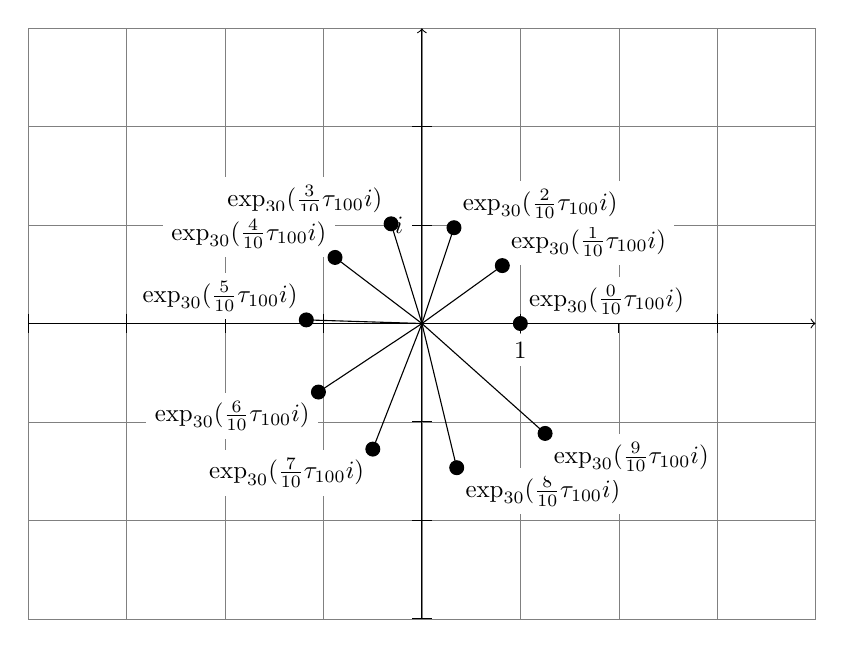
\begin{tikzpicture}[scale=1.25,every node/.style={scale=0.9}]
				    \draw[step=1,help lines] (-4.000000,-3.000000) grid (4.000000,3.000000);
            \draw[->] (-4.000000,0) -- (4.000000,0);
            \draw[->] (0,-3.000000) -- (0,3.000000);
            \draw (-4.000000, 0.100000) -- (-4.000000,-0.100000);
            \draw (-3.000000, 0.100000) -- (-3.000000,-0.100000);
            \draw (-2.000000, 0.100000) -- (-2.000000,-0.100000);
            \draw (-1.000000, 0.100000) -- (-1.000000,-0.100000);
            \draw (0.000000, 0.100000) -- (0.000000,-0.100000);
            \draw (1.000000, 0.100000) -- (1.000000,-0.100000);
            \draw (2.000000, 0.100000) -- (2.000000,-0.100000);
            \draw (3.000000, 0.100000) -- (3.000000,-0.100000);
            \draw (0.100000, -3.000000) -- (-0.100000,-3.000000);
            \draw (0.100000, -2.000000) -- (-0.100000,-2.000000);
            \draw (0.100000, -1.000000) -- (-0.100000,-1.000000);
            \draw (0.100000, 0.000000) -- (-0.100000,0.000000);
            \draw (0.100000, 1.000000) -- (-0.100000,1.000000);
            \draw (0.100000, 2.000000) -- (-0.100000,2.000000);
            \draw (1,-0.100000) node[anchor=north,fill=white]{$1$};
            \draw (-0.100000,1) node[anchor=east,fill=white]{$i$};
            \draw (1.000000,0.000000) node[anchor=south west,fill=white]{$\exp_{30}(\frac{0}{10}\tau_{100}i)$};
            \filldraw (1.000000,0.000000) circle (2pt);
            \draw (0,0) -- (1.000000,0.000000);
            \draw (0.816701,0.588280) node[anchor=south west,fill=white]{$\exp_{30}(\frac{1}{10}\tau_{100}i)$};
            \filldraw (0.816701,0.588280) circle (2pt);
            \draw (0,0) -- (0.816701,0.588280);
            \draw (0.325644,0.973269) node[anchor=south west,fill=white]{$\exp_{30}(\frac{2}{10}\tau_{100}i)$};
            \filldraw (0.325644,0.973269) circle (2pt);
            \draw (0,0) -- (0.325644,0.973269);
            \draw (-0.313007,1.012825) node[anchor=south east,fill=white]{$\exp_{30}(\frac{3}{10}\tau_{100}i)$};
            \filldraw (-0.313007,1.012825) circle (2pt);
            \draw (0,0) -- (-0.313007,1.012825);
            \draw (-0.882924,0.671288) node[anchor=south east,fill=white]{$\exp_{30}(\frac{4}{10}\tau_{100}i)$};
            \filldraw (-0.882924,0.671288) circle (2pt);
            \draw (0,0) -- (-0.882924,0.671288);
            \draw (-1.174740,0.036654) node[anchor=south east,fill=white]{$\exp_{30}(\frac{5}{10}\tau_{100}i)$};
            \filldraw (-1.174740,0.036654) circle (2pt);
            \draw (0,0) -- (-1.174740,0.036654);
            \draw (-1.051451,-0.696467) node[anchor=north east,fill=white]{$\exp_{30}(\frac{6}{10}\tau_{100}i)$};
            \filldraw (-1.051451,-0.696467) circle (2pt);
            \draw (0,0) -- (-1.051451,-0.696467);
            \draw (-0.498924,-1.276177) node[anchor=north east,fill=white]{$\exp_{30}(\frac{7}{10}\tau_{100}i)$};
            \filldraw (-0.498924,-1.276177) circle (2pt);
            \draw (0,0) -- (-0.498924,-1.276177);
            \draw (0.353481,-1.464927) node[anchor=north west,fill=white]{$\exp_{30}(\frac{8}{10}\tau_{100}i)$};
            \filldraw (0.353481,-1.464927) circle (2pt);
            \draw (0,0) -- (0.353481,-1.464927);
            \draw (1.251358,-1.116865) node[anchor=north west,fill=white]{$\exp_{30}(\frac{9}{10}\tau_{100}i)$};
            \filldraw (1.251358,-1.116865) circle (2pt);
            \draw (0,0) -- (1.251358,-1.116865);
			    \end{tikzpicture}
		    \end{minipage}
		    \begin{minipage}[c]{0.35\textwidth}
			    A plot of the list of complex numbers $\exp_{30}(\frac{[0:11]}{10}\tau_{100}i)$. Notice that when measurements are done relative to the complex number $1$, $\exp_{30}(\frac{1}{10}\tau_{100}i)$ is roughly $\frac{1}{10}$\textsuperscript{th} of a revolution, and also that each complex number has an angle that is roughly an integral multiple of that of $\exp_{30}(\frac{1}{10}\tau_{100}i)$.
		    \end{minipage}
	    \begin{multicols*}{2}
		    \procedure{3.90}
			    \objective
				    Choose a two rationals $M,N$ such that $0<M$ and $N^2<12$. The objective of the following instructions is to construct rational numbers $a,b$ such that $a>0$, and a procedure, $p(x,n)$, to show that $\lVert\cos_n(x)-1\rVert^2\ge a^2$ when a rational number $x$ and a positive integer $n$ such that $M\le\lvert x\rvert\le N$ and $n>b$ are chosen.
			    \implementation
				    \begin{enumerate}
					    \item Let $a=\frac{M^2}{4}(1-\frac{N^2}{12})$.
					    \item \textbf{Verify that $a>0$.}
					    \item Let $b=4$.
					    \item Let $p(x,n)$ be the following procedure:
					    \begin{enumerate}
						    \item Using \procedurehr{3.22}, verify that $(\cos_n(x)-1)^2$
						    \begin{enumerate}
							    \item $=(\frac{1}{2}((1+\frac{xi}{n})^n+(1-\frac{xi}{n})^n)-1)^2$
							    \item $=(\frac{1}{2}(\sum_r^{[0:{n+1}]}\frac{n^{\ul{r}}}{r!}(\frac{x}{n})^ri^r+\sum_r^{[0:{n+1}]}\frac{n^{\ul{r}}}{r!}(\frac{x}{n})^r(-i)^r)-1)^2$
							    \item $=(\sum_r^{[0:\lfloor\frac{n}{2}\rfloor+1]}\frac{n^{\ul{2r}}}{(2r)!}(\frac{x}{n})^{2r}(-1)^r-1)^2$
							    \item $=(\sum_r^{[1:\lfloor\frac{n}{2}\rfloor+1]}\frac{n^{\ul{2r}}}{(2r)!}(\frac{x}{n})^{2r}(-1)^r)^2$
							    \item $=(\sum_r^{[1:\lfloor\frac{\lfloor\frac{n}{2}\rfloor}{2}\rfloor+1]}(-\frac{n^{\ul{4r-2}}}{(4r-2)!}(\frac{x}{n})^{4r-2}+\frac{n^{\ul{4r}}}{(4r)!}(\frac{x}{n})^{4r})-\frac{n^{\ul{2\lfloor\frac{n}{2}\rfloor}}}{(2\lfloor\frac{n}{2}\rfloor)!}(\frac{x}{n})^{2\lfloor\frac{n}{2}\rfloor}[\lfloor\frac{n}{2}\rfloor\bmod 2=1])^2$
							    \item $\ge(\sum_r^{[1:\lfloor\frac{\lfloor\frac{n}{2}\rfloor}{2}\rfloor+1]}\frac{n^{\ul{4r-2}}}{(4r-2)!}(\frac{x}{n})^{4r-2}(-1+\frac{(n-4r+2)^{\ul{2}}}{(4r)^{\ul{2}}}(\frac{x}{n})^{2}))^2$
							    \item $\ge(\sum_r^{[1:\lfloor\frac{\lfloor\frac{n}{2}\rfloor}{2}\rfloor+1]}\frac{n^{\ul{4r-2}}}{(4r-2)!}(\frac{x}{n})^{4r-2}(-1+\frac{1}{(4r)^{\ul{2}}}(x)^{2}))^2$
							    \item $\ge(\sum_r^{[1:\lfloor\frac{\lfloor\frac{n}{2}\rfloor}{2}\rfloor+1]}\frac{n^{\ul{4r-2}}}{(4r-2)!}(\frac{x}{n})^{4r-2}(-1+\frac{1}{12}x^{2}))^2$
							    \item $\ge(\sum_r^{[1:\lfloor\frac{\lfloor\frac{n}{2}\rfloor}{2}\rfloor+1]}\frac{n^{\ul{4r-2}}}{(4r-2)!}(\frac{x}{n})^{4r-2}(-1+\frac{N^2}{12}))^2$
							    \item $\ge(\frac{n^{\ul{2}}}{2}(\frac{x}{n})^{2}(-1+\frac{N^2}{12}))^2$
							    \item $\ge(\frac{1}{4}x^{2}(-1+\frac{N^2}{12}))^2$
							    \item $\ge(\frac{M^2}{4}(-1+\frac{N^2}{12}))^2$
							    \item $=a^2$
						    \end{enumerate}
					    \end{enumerate}
					    \item \textbf{Yield the tuple $\langle a,b,p\rangle$.}
				    \end{enumerate}
		    \procedure{3.60}
			    \objective
				    Choose a positive integer $K$. The objective of the following instructions is to construct rational numbers $a,b,c$ such that $a>0$, and a procedure, $p(n,m,k)$, to show that $\lVert\exp_n(\frac{k}{K}\tau_mi)-1\rVert^2\ge a^2$ when an integer $k$ and positive integers $n,m$ such that $0<\lvert k\rvert\le\frac{K}{2}$, $n>b$, and $m>c$ are chosen.
			    \implementation
				    \begin{enumerate}
					    \item Execute \procedurehr{3.50} and let $\langle a_1,c,p_1\rangle$ receive.
					    \item Verify that $(\frac{a_1}{2})^2<12$.
					    \item Execute \procedurehr{3.49} and let $\langle a_2,p_2\rangle$ receive.
					    \item Verify that $a_2>0$.
					    \item Execute \procedurehr{3.90} on $\langle\frac{a_2}{K},\frac{a_1}{2}\rangle$ and let $\langle a,b,p_3\rangle$ receive.
					    \item \textbf{Verify that $a>0$.}
					    \item Let $p(n,m,k)$ be the following procedure:
					    \begin{enumerate}
						    \item Verify that $1\le\lvert k\rvert\le\frac{K}{2}$.
						    \item Hence verify that $\frac{1}{K}\le\frac{\lvert k\rvert}{K}\le\frac{1}{2}$.
						    \item Execute procedure $p_1$ on $\langle m\rangle$.
						    \item Execute procedure $p_2$ on $\langle m\rangle$.
						    \item Hence verify that $0<\frac{a_2}{K}\le\frac{1}{K}\tau_m\le\frac{\lvert k\rvert}{K}\tau_m\le\frac{1}{2}\tau_m\le\frac{a_1}{2}$.
						    \item Hence execute procedure $p_3$ on $\langle\frac{k}{K}\tau_m,n\rangle$.
						    \item Hence verify that $(\cos_n(\frac{k}{K}\tau_m)-1)^2\ge a^2$.
						    \item Using \procedurehr{3.22}, verify that $\lVert\exp_n(\frac{k}{K}\tau_mi)-1\rVert^2$
						    \begin{enumerate}
							    \item $\ge\Re(\exp_n(\frac{k}{K}\tau_mi)-1)^2$
							    \item $=(\cos_n(\frac{k}{K}\tau_m)-1)^2$
							    \item $\ge a^2$
						    \end{enumerate}
					    \end{enumerate}
					    \item \textbf{Yield the tuple $\langle a,b,c,p\rangle$.}
				    \end{enumerate}
		    \procedure{3.61}
			    \objective
				    Choose a positive integer $K$. The objective of the following instructions is to construct rational numbers $a,b,c$ such that $a>0$, and a procedure, $p(n,m,j,k)$, to show that $\lVert\exp_n(\frac{k}{K}\tau_mi)-\exp_n(\frac{j}{K}\tau_mi)\rVert^2\ge a^2$ when positive integers $n,j,k,m$ such that $-K<j\le k<K$, $0<k-j\le\frac{K}{2}$, $n\ge b$, and $m\ge c$ are chosen.
			    \implementation
				    \begin{enumerate}
					    \item Execute \procedurehr{3.50} and let $\langle a_1,b_1,p_1\rangle$ receive.
					    \item Execute \procedurehr{3.14} on $\langle a_1\rangle$ and let $\langle a_2,b_2,p_2\rangle$ receive.
					    \item Execute \procedurehr{3.60} on $\langle K\rangle$ and let $\langle a_3,b_3,c_3,p_3\rangle$ receive.
					    \item Execute \procedurehr{3.15} on $\langle a_1\rangle$ and let $\langle a_4,b_4,p_4\rangle$ receive.
					    \item Let $a=\frac{1}{2}a_2a_3$.
					    \item Let $b=\max(\frac{2a_4{a_1}^2}{a_2a_3},b_3,b_4,b_2)$.
					    \item Let $c=\max(b_1,c_3)$.
					    \item Let $p(n,m,j,k)$ be the following procedure:
					    \begin{enumerate}
						    \item Verify that $-K<j<K$.
						    \item Hence verify that $-1<\frac{j}{K}<1$.
						    \item Hence verify that $\lVert\frac{j}{K}\rVert^2<1$.
						    \item Execute procedure $p_1$ on $\langle m\rangle$.
						    \item Hence verify that $\lVert\frac{j}{K}\tau_mi\rVert^2=\lVert\frac{j}{K}\rVert^2\lVert\tau_m\rVert^2\le\lVert\tau_m\rVert^2\le{a_1}^2$.
						    \item Execute procedure $p_2$ on $\langle\frac{j}{K}\tau_mi,n\rangle$.
						    \item Hence verify that $\lVert\exp_n(\frac{j}{K}\tau_mi)\rVert^2\ge{a_2}^2>0$.
						    \item Execute procedure $p_3$ on $\langle n,m,k-j\rangle$.
						    \item Hence verify that $\lVert\exp_n(\frac{k-j}{K}\tau_mi)-1\rVert^2\ge{a_3}^2>0$.
						    \item Verify that $0<\frac{k-j}{K}\le\frac{1}{2}$.
						    \item Hence verify that $\lVert\frac{k-j}{K}\tau_mi\rVert^2\le\lVert\frac{k-j}{K}\rVert^2\lVert\tau_m\rVert^2\le\lVert\tau_m\rVert^2\le{a_1}^2$.
						    \item Verify that $n\ge b\ge\frac{2a_4{a_1}^2}{a_2a_3}$.
						    \item Execute procedure $p_4$ on $\langle\frac{k-j}{K}\tau_mi,\frac{j}{K}\tau_mi,n\rangle$.
						    \item Hence verify that $\lVert\exp_n(\frac{k-j}{K}\tau_mi)\exp_n(\frac{j}{K}\tau_mi)-\exp_n(\frac{k-j}{K}\tau_mi+\frac{j}{K}\tau_mi)\rVert^2\le\frac{{a_4}^2\lVert\frac{k-j}{K}\tau_mi\rVert^2\lVert\frac{j}{K}\tau_mi\rVert^2}{n^2}\le\frac{{a_4}^2{a_1}^4}{n^2}\le(\frac{a_2a_3}{2})^2$.
						    \item Hence using \procedurehr{sat1708191238}, verify that $\lVert\exp_n(\frac{k}{K}\tau_mi)-\exp_n(\frac{j}{K}\tau_mi)\rVert^2$
						    \begin{enumerate}
							    \item $=\lVert\exp_n(\frac{k-j}{K}\tau_mi+\frac{j}{K}\tau_mi)-\exp_n(\frac{k-j}{K}\tau_mi)\exp_n(\frac{j}{K}\tau_mi)+\exp_n(\frac{k-j}{K}\tau_mi)\exp_n(\frac{j}{K}\tau_mi)-\exp_n(\frac{j}{K}\tau_mi)\rVert^2$
							    \item $=\lVert\exp_n(\frac{j}{K}\tau_mi)(\exp_n(\frac{k-j}{K}\tau_mi)-1)-(\exp_n(\frac{k-j}{K}\tau_mi+\frac{j}{K}\tau_mi)-\exp_n(\frac{k-j}{K}\tau_mi)\exp_n(\frac{j}{K}\tau_mi))\rVert^2$
							    \item $\ge (a_2a_3-\frac{a_2a_3}{2})^2$
							    \item $\ge a^2$.
						    \end{enumerate}
					    \end{enumerate}
					    \item \textbf{Yield the tuple $\langle a,b,c,p\rangle$.}
				    \end{enumerate}
		    \procedure{3.62}
			    \objective
				    Choose a positive integer $K$. The objective of the following instructions is to construct rational numbers $a,b,c$ such that $a>0$, and a procedure, $p(n,m,j,k)$, to show that $\lVert\exp_n(\frac{k}{K}\tau_mi)-\exp_n(\frac{j}{K}\tau_mi)\rVert^2\ge a^2$ when positive integers $n,j,k,m$ such that $0\le j\le k<K$, $\frac{K}{2}\le k-j<K$, $n\ge b$, and $\frac{m}{n}\ge c$ are chosen.
			    \implementation
				    \begin{enumerate}
					    \item Execute \procedurehr{3.61} on $\langle K\rangle$ and let $\langle a_1,b_1,c_1,p_1\rangle$ receive.
					    \item Execute \procedurehr{3.50} and let $\langle a_2,b_2,p_2\rangle$ receive.
					    \item Execute \procedurehr{3.59} on $\langle a_2,4\rangle$ and let $\langle a_3,b_3,c_3,d_3,p_3\rangle$ receive.
					    \item Let $a=\frac{1}{2}a_1$.
					    \item Let $b=\max(\frac{4b_3}{a_1},b_1,c_3)$.
					    \item Let $c=\max(\frac{4a_3}{a_1},\frac{c_1}{b},\frac{b_2}{b},\frac{d_3}{b})$.
					    \item Let $p(n,m,j,k)$ be the following procedure:
					    \begin{enumerate}
						    \item Verify that $-\frac{K}{2}\le k-K<j<\frac{K}{2}$.
						    \item Also verify that $0<j-(k-K)\le\frac{K}{2}$.
						    \item Verify that $m\ge cn\ge\frac{c_1}{b}b=c_1$.
						    \item Hence execute procedure $p_1$ on $\langle n,m,k-K,j\rangle$.
						    \item Hence verify that $\lVert\exp_n(\frac{j}{K}\tau_mi)-\exp_n(\frac{k-K}{K}\tau_mi)\rVert^2\ge{a_1}^2$.
						    \item Verify that $m\ge cn\ge\frac{b_2}{b}b=b_2$.
						    \item Execute procedure $p_2$ on $\langle m\rangle$.
						    \item Hence verify that $\tau_m\le a_2$.
						    \item Hence verify that $\lVert\frac{k}{K}\tau_mi\rVert^2=\lVert\frac{k}{K}\rVert^2\lVert\tau_m\rVert^2\le\lVert\tau_m\rVert^2\le{a_2}^2$.
						    \item Also verify that $m\ge cn\ge\frac{d_3}{b}b=d_3$.
						    \item Now execute procedure $p_3$ on $\langle\frac{k}{K}\tau_mi,n,m,-4\rangle$.
						    \item Hence verify that $\lVert i^{-4}\exp_n(\frac{k}{K}\tau_mi)-\exp_n(\frac{k}{K}\tau_mi-\frac{4}{4}\tau_mi)\rVert^2\le(\frac{a_3n}{m}+\frac{b_3}{n})^2\le(\frac{a_1}{2})^2$.
						    \item Now verify that $\lVert\exp_n(\frac{k}{K}\tau_mi)-\exp_n(\frac{j}{K}\tau_mi)\rVert^2$
						    \begin{enumerate}
							    \item $=\lVert\exp_n(\frac{k}{K}\tau_mi)-\exp_n(\frac{k}{K}\tau_mi-\tau_mi)+\exp_n(\frac{k-K}{K}\tau_mi)-\exp_n(\frac{j}{K}\tau_mi)\rVert^2$
							    \item $\ge\frac{1}{2}\lVert\exp_n(\frac{k-K}{K}\tau_mi)-\exp_n(\frac{j}{K}\tau_mi)\rVert^2-\lVert\exp_n(\frac{k}{K}\tau_mi)-\exp_n(\frac{k}{K}\tau_mi-\tau_mi)\rVert^2$
							    \item $\ge\frac{1}{2}{a_1}^2-(\frac{a_1}{2})^2$
							    \item $\ge a^2$.
						    \end{enumerate}
					    \end{enumerate}
					    \item \textbf{Yield the tuple $\langle a,b,c,p\rangle$.}
				    \end{enumerate}
		    \procedure{3.63}
			    \objective
				    Choose a positive integer $K$. The objective of the following instructions is to construct rational numbers $a,b,c$ such that $a>0$, and a procedure, $p(n,m,j,k)$, to show that $\lVert\exp_n(\frac{k}{K}\tau_mi)-\exp_n(\frac{j}{K}\tau_mi)\rVert^2\ge a^2$ when positive integers $n,j,k,m$ such that $0\le j\le k<K$, $0<k-j<K$, $n\ge b$, and $\frac{m}{n}\ge c$ are chosen.
			    \implementation
				    \begin{enumerate}
					    \item Execute \procedurehr{3.61} on $\langle K\rangle$ and let $\langle a_1,b_1,c_1,p_1\rangle$ receive.
					    \item Execute \procedurehr{3.62} on $\langle K\rangle$ and let $\langle a_2,b_2,c_2,p_2\rangle$ receive.
					    \item Let $a=\min(a_1,a_2)$.
					    \item \textbf{Verify that $a>0$.}
					    \item Let $b=\max(b_1,b_2)$.
					    \item Let $c=\max(\frac{c_1}{b},c_2)$.
					    \item Let $p(n,m,j,k)$ be the following procedure:
					    \begin{enumerate}
						    \item If $k-j\le\frac{K}{2}$, then do the following:
						    \begin{enumerate}
						      \item Verify that $m\ge cn\ge\frac{c_1}{b}b=c_1$.
							    \item Execute procedure $p_1$ on $\langle n,m,j,k\rangle$.
							    \item \textbf{Hence verify that $\lVert\exp_n(\frac{k}{K}\tau_mi)-\exp_n(\frac{j}{K}\tau_mi)\rVert^2\ge a_1\ge a$.}
						    \end{enumerate}
						    \item Otherwise if $k-j>\frac{K}{2}$, then do the following:
						    \begin{enumerate}
							    \item Execute procedure $p_2$ on $\langle n,m,j,k\rangle$.
							    \item \textbf{Hence verify that $\lVert\exp_n(\frac{k}{K}\tau_mi)-\exp_n(\frac{j}{K}\tau_mi)\rVert^2\ge a_2\ge a$.}
						    \end{enumerate}
					    \end{enumerate}
					    \item \textbf{Yield the tuple $\langle a,b,c,p\rangle$.}
				    \end{enumerate}
		    \declaration{3.34}
			    The phrase "\gls{complexpolynomial}" will be used to indicate that the declarations and procedures pertaining to polynomials are being used but with the provison that all uses of rational numbers therein are substituted with uses of complex numbers.
		    \procedure{3.64}
			    \objective
				    Choose a positive integer $K$. The objective of the following instructions is to construct rational numbers $a,b,c,d$, and a procedure, $p(n,m)$, to construct a list of complex numbers $z$ and a list of complex polynomials $q$ such that,
				    \begin{enumerate}
					    \item $z_k=\exp_n(\frac{k}{K}\tau_mi)$ for $k\in[0:K]$
					    \item $q_K=\lambda^K-1$
					    \item $q_{K-1}=\sum_r^{[0:K]}\lambda^r$
					    \item $q_{k+1}=(\lambda-z_k)q_k+\Lambda(q_{k+1},z_k)$ for $k\in[0:K]$
					    \item $(q_k)_{\deg(q_k)}=1$ for $k\in[0:K+1]$
					    \item $\Lambda(q_k,z_j)\equiv 0\err{\frac{an}{m}+\frac{b}{n}}$ for $j\in[0:k]$, for $k\in[0:K+1]$
				    \end{enumerate}
				    when two positive integers $n,m$ such that $n>c$ and $\frac{m}{n}>d$ are chosen.
			    \implementation
				    \begin{enumerate}
					    \item Execute \procedurehr{3.89} on $\langle K\rangle$ and let $\langle a_1,b_1,c_1,d_1,p_1\rangle$ receive.
					    \item Execute \procedurehr{3.63} on $\langle K\rangle$ and let $\langle a_2,b_2,c_2,p_2\rangle$ receive.
					    \item Let $a=\max(1,\frac{2}{a_2})^Ka_1$.
					    \item Let $b=\max(1,\frac{2}{a_2})^Kb_1$.
					    \item Let $c=\max(c_1,b_2)$.
					    \item Let $d=\max(d_1,c_2)$.
					    \item Let $p(n,m)$ be the following procedure:
					    \begin{enumerate}
						    \item \textbf{Let $q_K=\lambda^K-1$.}
						    \item For $k\in[K:0]$, do the following:
						    \begin{enumerate}
							    \item \textbf{Let $z_k=\exp_n(\frac{k}{K}\tau_mi)$.}
							    \item Execute procedure $p_1$ on $\langle n,m,k\rangle$.
							    \item \textbf{Hence verify that $\lVert\Lambda(q_K,z_k)\rVert^2\le(\frac{a_1n}{m}+\frac{b_1}{n})^2$.}
						    \end{enumerate}
						    \item For $k\in[K:0]$, do the following:
						    \begin{enumerate}
							    \item Let $q_k=q_{k+1}\div(\lambda-z_k)$.
							    \item Let $r_k=q_{k+1}\bmod(\lambda-z_k)$.
							    \item Verify that $\deg(r_k)<\deg(\lambda-z_k)=1$.
							    \item Hence verify that $\deg(r_k)=0$.
							    \item Verify that $q_{k+1}=(\lambda-z_k)q_k+r_k$.
							    \item \textbf{Hence verify that $1=(q_{k+1})_{\deg(q_{k+1})}=((\lambda-z_k)q_k+r_k)_{\deg(q_{k+1})}=(q_k)_{\deg(q_k)}$.}
							    \item Also verify that $\Lambda(q_{k+1},z_k)=\Lambda(\lambda-z_k,z_k)\Lambda(q_k,z_k)+\Lambda(r_k,z_k)=(z_k-z_k)\Lambda(q_k,z_k)+r_k=r_k$.
							    \item \textbf{Hence verify that $q_{k+1}=(\lambda-z_k)q_k+\Lambda(q_{k+1},z_k)$.}
							    \item Execute the \subprocedurehr{wed2808191630} on $\langle k,q_{k+1},z\rangle$.
							    \item Now using (cvii), verify that $(\lambda-1)\sum_r^{[0:K]}\lambda^r$
							    \begin{enumerate}
								    \item $=q_K$
								    \item $=(\lambda-z_{K-1})q_{K-1}+\Lambda(q_K,z_{K-1})$
								    \item $=(\lambda-1)q_{K-1}+\Lambda(\lambda^K-1,1)$
								    \item $=(\lambda-1)q_{K-1}$.
							    \end{enumerate}
							    \item \textbf{Hence verify that $\sum_r^{[0:K]}\lambda^r=q_{K-1}$.}
						    \end{enumerate}
						    \item \textbf{Yield the tuple $\langle z,q\rangle$.}
					    \end{enumerate}
					    \item \textbf{Yield the tuple $\langle a,b,c,d,p\rangle$.}
				    \end{enumerate}
			    \subprocedure{wed2808191630}
			      \paragraph{Objective}
			        Choose a non-negative integer $k$, a complex polynomial $q_{k+1}$, and a list of complex numbers $z$ such that $z_j=\exp_n(\frac{j}{K}\tau_mi)$ and $\Lambda(q_{k+1},z_j)\equiv 0\err{(\frac{2}{a_2})^{K-(k+1)}(\frac{a_1n}{m}+\frac{b_1}{n})}$ for $j\in[k+1:0]$. Let $q_k=q_{k+1}\div(\lambda-z_k)$. The objective of the following instructions is to show that $\Lambda(q_{k},z_j)\equiv 0\err{(\frac{2}{a_2})^{K-k}(\frac{a_1n}{m}+\frac{b_1}{n})}\err{\frac{an}{m}+\frac{b}{n}}$ for $j\in[k:0]$.
			      \paragraph{Implementation}
			        \begin{enumerate}
			          \item For $j\in[k:0]$, do the following:
						    \begin{enumerate}
							    \item Verify that $\Lambda(q_{k+1},z_j)=\Lambda(\lambda-z_k,z_j)\Lambda(q_k,z_j)+\Lambda(q_{k+1},z_k)$.
							    \item Hence verify that $\Lambda(q_{k+1},z_j)-\Lambda(q_{k+1},z_k)=(z_j-z_k)\Lambda(q_k,z_j)$.
							    \item Execute procedure $p_2$ on $\langle n,m,\min(j,k),\max(j,k)\rangle$.
							    \item Hence verify that $\lVert z_j-z_k\rVert^2\ge {a_2}^2$.
							    \item Hence verify that ${a_2}^2\lVert\Lambda(q_k,z_j)\rVert^2$
							    \begin{enumerate}
							      \item $\le\lVert z_j-z_k\rVert^2\lVert\Lambda(q_k,z_j)\rVert^2$
							      \item $=\lVert(z_j-z_k)\Lambda(q_k,z_j)\rVert^2$
							      \item $=\lVert\Lambda(q_{k+1},z_j)-\Lambda(q_{k+1},z_k)\rVert^2$
							      \item $\le((\frac{2}{a_2})^{K-k-1}(\frac{a_1n}{m}+\frac{b_1}{n})+(\frac{2}{a_2})^{K-k-1}(\frac{a_1n}{m}+\frac{b_1}{n}))^2$
							      \item $=(2(\frac{2}{a_2})^{K-k-1}(\frac{a_1n}{m}+\frac{b_1}{n}))^2$
							      \item $={a_2}^2((\frac{2}{a_2})^{K-k}(\frac{a_1n}{m}+\frac{b_1}{n}))^2$.
							    \end{enumerate}
							    \item \textbf{Hence verify that $\lVert\Lambda(q_k,z_j)\rVert^2\le((\frac{2}{a_2})^{K-k}(\frac{a_1n}{m}+\frac{b_1}{n}))^2\le(\frac{an}{m}+\frac{b}{n})^2$.}
						    \end{enumerate}
					    \end{enumerate}
		    \procedure{3.65}
			    \objective
				    Choose a rational number $X$ and a positive integer $K$. The objective of the following instructions is to construct rational numbers $a,b,c,d$, and a procedure, $p(x,n,m)$, to show that $\sum_r^{[0:K]}x^r\equiv\prod_r^{[1:K]}(x-\exp_n(\frac{r}{K}\tau_mi))\err{\frac{an}{m}+\frac{b}{n}}$ when a complex number $x$ and positive integers $n,m$ such that $n>c$, $\frac{m}{n}>d$, and $\lVert x\rVert^2\le X$ are chosen.
			    \implementation
				    \begin{enumerate}
					    \item Execute \procedurehr{3.64} on $\langle K\rangle$ and let $\langle a_1,b_1,c_1,d_1,p_1\rangle$ receive.
					    \item Execute \procedurehr{3.50} and let $\langle a_2,b_2,p_2\rangle$ receive.
					    \item Execute \procedurehr{3.13} on $\langle a_2\rangle$ and let $\langle a_3,b_3,p_3\rangle$ receive.
					    \item Let $l=\sum_k^{[0:K-1]}\prod_j^{[k+1:K-1]}(X+a_3)$.
					    \item Let $a=a_1l$.
					    \item Let $b=b_1l$.
					    \item Let $c=\max(c_1,b_3)$.
					    \item Let $d=\max(d_1,b_2)$.
					    \item Let $p(x,n,m)$ be the following procedure:
					    \begin{enumerate}
						    \item Execute procedure $p_2$ on $\langle m\rangle$.
						    \item Hence verify that $\tau_m\le a_2$.
						    \item Execute procedure $p_1$ on $\langle n,m\rangle$ and let $\langle z,t\rangle$ receive.
						    \item For $j\in[1:K]$, do the following:
						    \begin{enumerate}
							    \item Verify that $\lVert\frac{j}{K}\tau_mi\rVert^2=\lVert\frac{j}{K}\rVert^2\lVert\tau_m\rVert^2\le\lVert\tau_m\rVert^2\le a_2$.
							    \item Execute procedure $p_3$ on $\langle\frac{j}{K}\tau_mi,n\rangle$.
							    \item Hence verify that $\lVert z_j\rVert^2=\lVert\exp_n(\frac{j}{K}\tau_mi)\rVert^2\le a_3$.
						    \end{enumerate}
						    \item Hence verify that $\lVert\sum_r^{[0:K]}x^r-\prod_r^{[1:K]}(x-z_r)\rVert^2$
						    \begin{enumerate}
							    \item $=\lVert\Lambda(\sum_r^{[0:K]}\lambda^r,x)-\prod_r^{[1:K]}(x-z_r)\rVert^2$
							    \item $=\lVert\Lambda(t_{K-1},x)-\prod_r^{[1:K]}(x-z_r)\rVert^2$
							    \item $=\lVert\Lambda(\prod_j^{[0:K-1]}(\lambda-z'_j)+\sum_k^{[0:K-1]}\Lambda(t_{k+1},z'_{k})\prod_j^{[k+1:K-1]}(\lambda-z'_j),x)-\prod_r^{[1:K]}(x-z_r)\rVert^2$
							    \item $=\lVert\prod_j^{[0:K-1]}(x-z'_j)+\sum_k^{[0:K-1]}\Lambda(t_{k+1},z'_{k})\prod_j^{[k+1:K-1]}(x-z'_j)-\prod_r^{[1:K]}(x-z_r)\rVert^2$
							    \item $=\lVert\sum_k^{[0:K-1]}\Lambda(t_{k+1},z'_{k})\prod_j^{[k+1:K-1]}(x-z'_j)\rVert^2$
							    \item $\le(\sum_k^{[0:K-1]}(\frac{a_1n}{m}+\frac{b_1}{n})\prod_j^{[k+1:K-1]}(X+a_3))^2$
							    \item $=((\frac{a_1n}{m}+\frac{b_1}{n})\sum_k^{[0:K-1]}\prod_j^{[k+1:K-1]}(X+a_3))^2$
							    \item $=(\frac{an}{m}+\frac{b}{n})^2$.
						    \end{enumerate}
					    \end{enumerate}
					    \item \textbf{Yield the tuple $\langle a,b,c,d,p\rangle$.}
				    \end{enumerate}
		    \procedure{3.66}
			    \objective
				    Choose a rational number $X$ and a positive integer $K$. The objective of the following instructions is to construct rational numbers $a,b,c,d$, and a procedure, $p(x,n,m)$, to show that $x^K-1\equiv\prod_r^{[0:K]}(x-\exp_n(\frac{r}{K}\tau_mi))\err{\frac{an}{m}+\frac{b}{n}}$ when a complex number $x$ and positive integers $n,m$ such that $n>c$, $\frac{m}{n}>d$, and $\lVert x\rVert^2\le X$ are chosen.
			    \implementation
				    \begin{enumerate}
					    \item Execute \procedurehr{3.65} on $\langle X,K\rangle$ and let $\langle a_1,b_1,c,d,p_1\rangle$ receive.
					    \item Let $a=(X+1)a_1$.
					    \item Let $b=(X+1)b_1$.
					    \item Let $p(x,n,m)$ be the following procedure:
					    \begin{enumerate}
						    \item Execute procedure $p_1$ on $\langle x,n,m\rangle$.
						    \item Hence verify that $\lVert\sum_r^{[0:K]}x^r-\prod_r^{[1:K]}(x-\exp_n(\frac{r}{K}\tau_mi))\rVert^2\le(\frac{a_1n}{m}+\frac{b_1}{n})^2$.
						    \item Hence verify that $\lVert x^K-1-\prod_r^{[0:K]}(x-\exp_n(\frac{r}{K}\tau_mi))\rVert^2$
						    \begin{enumerate}
							    \item $=\lVert(x-1)\sum_r^{[0:K]}x^r-(x-1)\prod_r^{[1:K]}(x-\exp_n(\frac{r}{K}\tau_mi))\rVert^2$
							    \item $=\lVert x-1\rVert^2\lVert\sum_r^{[0:K]}x^r-\prod_r^{[1:K]}(x-\exp_n(\frac{r}{K}\tau_mi))\rVert^2$
							    \item $\le(X+1)^2(\frac{a_1n}{m}+\frac{b_1}{n})^2$
							    \item $=(\frac{an}{m}+\frac{b}{n})^2$.
						    \end{enumerate}
					    \end{enumerate}
					    \item \textbf{Yield the tuple $\langle a,b,c,d,p\rangle$.}
				    \end{enumerate}
		    \procedure{3.67}
			    \objective
				    Choose a rational number $X$ and a positive integer $K$. The objective of the following instructions is to construct rational numbers $a,b,c,d$, and a procedure, $p(x,n,m)$, to show that $\exp_K(x)-1\equiv x\prod_r^{[1:K]}(1-\frac{x}{K(\exp_n(\frac{r}{K}\tau_mi)-1)})\err{\frac{an}{m}+\frac{b}{n}}$ when a complex number $x$ and positive integers $n,m$ such that $n>c$, $\frac{m}{n}>d$, and $\lVert x\rVert^2\le X$ are chosen.
			    \implementation
				    \begin{enumerate}
					    \item Execute \procedurehr{3.66} on $\langle 1+\frac{X}{K},K\rangle$ and let $\langle a_1,b_1,c_1,d_1,p_1\rangle$ receive.
					    \item Execute \procedurehr{3.65} on $\langle 1,K\rangle$ and let $\langle a_2,b_2,c_2,d_2,p_2\rangle$ receive.
					    \item Execute \procedurehr{3.63} on $\langle K\rangle$ and let $\langle a_3,b_3,c_3,p_3\rangle$ receive.
					    \item Let $l=\frac{X}{K}(1+\frac{X}{Ka_3})^{K-1}$.
					    \item Let $a=a_1+la_2$.
					    \item Let $b=b_1+lb_2$.
					    \item Let $c=\max(c_1,c_2,b_3)$.
					    \item Let $d=\max(d_1,d_2,c_3)$.
					    \item Let $p(x,n,m)$ be the following procedure:
					    \begin{enumerate}
						    \item Verify that $\lVert 1+\frac{x}{K}\rVert^2\le (1+\frac{X}{K})^2$.
						    \item Hence execute procedure $p_1$ on $\langle 1+\frac{x}{K},n,m\rangle$.
						    \item Hence verify that $\lVert(1+\frac{x}{K})^K-1-\prod_r^{[0:K]}(1+\frac{x}{K}-\exp_n(\frac{r}{K}\tau_mi))\rVert^2\le(\frac{a_1n}{m}+\frac{b_1}{n})^2$.
						    \item Execute procedure $p_2$ on $\langle 1,n,m\rangle$.
						    \item Hence verify that $\lVert K-\prod_r^{[1:K]}(1-\exp_n(\frac{r}{K}\tau_mi))\rVert^2=\sum_r^{[0:K]}1^r-\prod_r^{[1:K]}(1-\exp_n(\frac{r}{K}\tau_mi))\rVert^2\le(\frac{a_2n}{m}+\frac{b_2}{n})^2$.
						    \item For $j\in[1:K]$, do the following:
						    \begin{enumerate}
							    \item Execute procedure $p_3$ on $\langle n,m,0,j\rangle$.
							    \item Hence verify that $\lVert\exp_n(\frac{j}{K}\tau_mi)-1\rVert^2\ge{a_3}^2$.
							    \item Let $z_j=K(\exp_n(\frac{j}{K}\tau_mi)-1)$.
						    \end{enumerate}
						    \item Hence verify that $\lVert\exp_K(x)-1-x\prod_r^{[1:K]}(1-\frac{x}{z_r})\rVert^2$
						    \begin{enumerate}
							    \item $=\lVert\exp_K(x)-1-\prod_r^{[0:K]}(1+\frac{x}{K}-\exp_n(\frac{r}{K}\tau_mi))+\prod_r^{[0:K]}(1+\frac{x}{K}-\exp_n(\frac{r}{K}\tau_mi))-x\prod_r^{[1:K]}(1-\frac{x}{z_r})\rVert^2$
							    \item $=\lVert\exp_K(x)-1-\prod_r^{[0:K]}(1+\frac{x}{K}-\exp_n(\frac{r}{K}\tau_mi))+\frac{x}{K}\prod_r^{[1:K]}(1+\frac{x}{K}-\exp_n(\frac{r}{K}\tau_mi))-x\prod_r^{[1:K]}(1-\frac{x}{z_r})\rVert^2$
							    \item $=\lVert\exp_K(x)-1-\prod_r^{[0:K]}(1+\frac{x}{K}-\exp_n(\frac{r}{K}\tau_mi))+\frac{x}{K}\prod_r^{[1:K]}(1-\exp_n(\frac{r}{K}\tau_mi))\prod_r^{[1:K]}(1-\frac{x}{z_r})-x\prod_r^{[1:K]}(1-\frac{x}{z_r})\rVert^2$
							    \item $=\lVert(\exp_K(x)-1-\prod_r^{[0:K]}(1+\frac{x}{K}-\exp_n(\frac{r}{K}\tau_mi)))+\frac{x}{K}\prod_r^{[1:K]}(1-\frac{x}{z_r})(\prod_r^{[1:K]}(1-\exp_n(\frac{r}{K}\tau_mi))-K)\rVert^2$
							    \item $\le((\frac{a_1n}{m}+\frac{b_1}{n})+\frac{X}{K}(\prod_r^{[1:K]}(1+\frac{X}{Ka_3}))(\frac{a_2n}{m}+\frac{b_2}{n}))^2$
							    \item $=((\frac{a_1n}{m}+\frac{b_1}{n})+\frac{X}{K}(1+\frac{X}{Ka_3})^{K-1}(\frac{a_2n}{m}+\frac{b_2}{n}))^2$
							    \item $=(\frac{an}{m}+\frac{b}{n})^2$.
						    \end{enumerate}
					    \end{enumerate}
					    \item \textbf{Yield the tuple $\langle a,b,c,d,p\rangle$.}
				    \end{enumerate}
	    \end{multicols*}
	  \clearpage
	\part{Differential Arithmetic}
	  \chapter{Differential Arithmetic}
	    \begin{multicols*}{2}
	      \procedure{tue2008191129}
	        \objective
	          Choose the following:
	          \begin{enumerate}
	            \item A procedure $q_1(x,n)$ to show that $p_n(x)\equiv 0\err{a_1}$ when a complex number $x$ and a positive integer $n$ such that $P(x)$ and $n>c_1$ are chosen.
	            \item A procedure $q_2(x,n)$ to show that $t_n(x)\equiv 0\err{a_2}^2$ when a complex number $x$ and a positive integer $n$ such that $R(x)$ and $n>c_2$ are chosen.
	          \end{enumerate}
	          The objective of the following instructions is to construct the following:
	          \begin{enumerate}
	            \item Rational numbers $a_3,b_3$.
	            \item A procedure $q_3(x,n)$ to show that $p_n(x)+t_n(x)\equiv 0\err{a_3}$ when a complex number $x$ and a positive integer $n$ such that $P(x)$, $R(x)$, and $n>b_3$ are chosen.
	          \end{enumerate}
	        \implementation
	          \begin{enumerate}
	            \item Let $a_3=a_1+a_2$.
	            \item Let $b_3=\max(c_1,c_2)$.
	            \item Let $q_3(x,n)$ be the following procedure:
	            \begin{enumerate}
	              \item Execute procedure $q_1$ on $\langle x,n\rangle$.
	              \item Hence verify that $p_n(x)\equiv 0\err{a_1}$.
	              \item Execute procedure $q_2$ on $\langle x,n\rangle$.
	              \item Hence verify that $t_n(x)\equiv 0\err{a_2}$.
	              \item Hence verify that $p_n(x)+t_n(x)\equiv 0\err{a_1+a_2}\err{a_3}$.
	            \end{enumerate}
	            \item \textbf{Yield the tuple $\langle a_3,b_3,q_3\rangle$.}
	          \end{enumerate}
	      \procedure{tue2008191139}
	        \objective
	          Choose the following:
	          \begin{enumerate}
	            \item A procedure $q_1(x,n)$ to show that $p_n(x)\equiv 0\err{a_1}$ when a complex number $x$ and a positive integer $n$ such that $P(x)$ and $n>c_1$ are chosen.
	            \item A procedure $q_2(x,n)$ to show that $t_n(x)\equiv 0\err{a_2}$ when a complex number $x$ and a positive integer $n$ such that $R(x)$ and $n>c_2$ are chosen.
	          \end{enumerate}
	          The objective of the following instructions is to construct the following:
	          \begin{enumerate}
	            \item Rational numbers $a_3,b_3$.
	            \item A procedure $q_3(x,n)$ to show that $p_n(x)t_n(x)\equiv 0\err{a_3}$ when a complex number $x$ and a positive integer $n$ such that $P(x)$, $R(x)$, and $n>b_3$ are chosen.
	          \end{enumerate}
	        \implementation
	          Implementation is analogous to that of \procedurehr{tue2008191129}.
	      \declaration{tue2008190516}
	        The notation \gls{differentialtaxicab}, where $x$ is a complex number, will be used as a shorthand for $\lvert\Re(x)\rvert+\lvert\Im(x)\rvert$.
	      \procedure{tue2008190655}
	        \objective
	          Choose a complex number $a$ such that $\{a\}=0$. The objective of the following instructions is to show that $a=0$.
	        \implementation
	          \begin{enumerate}
	            \item Using \declarationhr{tue2008190516}, verify that $\lvert\Re(a)\rvert+\lvert\Im(a)\rvert=0$.
	            \item Verify that $\lvert\Re(a)\rvert\ge 0$.
	            \item Verify that $\lvert\Im(a)\rvert\ge 0$.
	            \item Hence verify that $\lvert\Re(a)\rvert=0$.
	            \item Hence verify that $\Re(a)=0$.
	            \item Also verify that $\lvert\Im(a)\rvert=0$.
	            \item Hence verify that $\Im(a)=0$.
	            \item \textbf{Hence verify that $a=0$.}
	          \end{enumerate}
	      \procedure{tue2008190520}
	        \objective
	          Choose a complex number $a$ and a rational number $b$. The objective of the following instructions is to show that $\{ba\}=\lvert b\rvert\{a\}$.
	        \implementation
	          \begin{enumerate}
	            \item Using \declarationhr{tue2008190516}, verify that $\{ba\}$
	            \begin{enumerate}
	              \item $=\lvert\Re(ba)\rvert+\lvert\Im(ba)\rvert$
	              \item $=\lvert b\Re(a)\rvert+\lvert b\Im(a)\rvert$
	              \item $=\lvert b\rvert(\lvert\Re(a)\rvert+\lvert\Im(a)\rvert)$
	              \item $=\lvert b\rvert\{a\}$.
	            \end{enumerate}
	          \end{enumerate}
	      \procedure{tue2008190540}
	        \objective
	          Choose two complex numbers $a,b$. The objective of the following instructions is to show that $\{a+b\}\le\{a\}+\{b\}$.
	        \implementation
	          \begin{enumerate}
	            \item Using \declarationhr{tue2008190516}, verify that $\{a+b\}$
	            \begin{enumerate}
	              \item $=\lvert\Re(a+b)\rvert+\lvert\Im(a+b)\rvert$
	              \item $=\lvert\Re(a)+\Re(b)\rvert+\lvert\Im(a)+\Im(b)\rvert$
	              \item $\le\lvert\Re(a)\rvert+\lvert\Re(b)\rvert+\lvert\Im(a)\rvert+\lvert\Im(b)\rvert$
	              \item $=\{a\}+\{b\}$.
	            \end{enumerate}
	          \end{enumerate}
	      \procedure{tue2008190546}
	        \objective
	          Choose two complex numbers $a,b$. The objective of the following instructions is to show that $\{ab\}\le\{a\}\{b\}$.
	        \implementation
	          \begin{enumerate}
	            \item Using \procedurehr{tue2008190540}, verify that $\{ab\}$
	            \begin{enumerate}
	              \item $=\{(\Re(a)+\Im(b)i)b\}$
	              \item $=\{\Re(a)b+\Im(a)bi\}$
	              \item $\le\{\Re(a)b\}+\{\Im(a)b\}$
	              \item $=(\lvert\Re(a)\rvert+\lvert\Im(a)\rvert)\{b\}$
	              \item $=\{a\}\{b\}$.
	            \end{enumerate}
	          \end{enumerate}
	      \procedure{tue2008190632}
	        \objective
	          Choose a complex number $a$. The objective of the following instructions is to show that $\lVert a\rVert^2\le\{a\}^2$.
	        \implementation
	          \begin{enumerate}
	            \item Using \procedurehr{3.04aa}, verify that $\lVert a\rVert^2$
	            \begin{enumerate}
	              \item $=\lVert\Re(a)+\Im(a)i\rVert^2$
	              \item $\le(\lvert\Re(a)\rvert+\lvert\Im(a)\rvert)^2$
	              \item $=\{a\}^2$.
	            \end{enumerate}
	          \end{enumerate}
	      \procedure{tue2008190639}
	        \objective
	          Choose a complex number $a$. The objective of the following instructions is to show that $\{a\}^2\le 2\lVert a\rVert^2$.
	        \implementation
	          \begin{enumerate}
	            \item Verify that $2\lVert a\rVert^2-\{a\}^2$
	            \begin{enumerate}
	              \item $=2\Re(a)^2+2\Im(a)^2-(\lvert\Re(a)\rvert+\lvert\Im(a)\rvert)^2$
	              \item $=2\Re(a)^2+2\Im(a)^2-\Re(a)^2-2\lvert\Re(a)\rvert\lvert\Im(a)\rvert-\Im(a)^2$
	              \item $=\Re(a)^2-2\lvert\Re(a)\rvert\lvert\Im(a)\rvert+\Im(a)^2$
	              \item $=(\lvert\Re(a)\rvert-\lvert\Im(a)\rvert)^2$
	              \item $\ge 0$.
	            \end{enumerate}
	            \item \textbf{Hence verify that $\{a\}^2\le 2\lVert a\rVert^2$.}
	          \end{enumerate}
	      \declaration{3.29}
			    The notation \gls{differentialdiff}, where $x,z$ are complex numbers such that $z\ne 0$ and $f[x]$ is a function of $x$, will be used as a shorthand for $\frac{f(y+z)-f(y)}{z}$.
		    \procedure{3.83}
			    \objective
				    Choose two functions $f[x],g[x]$ and two complex numbers $y,z$ such that $z\ne 0$. The objective of the following instructions is to show that $\diff_{x=y}^z(f(x)+g(x))=\diff_{x=y}^zf(x)+\diff_{x=y}^zg(x)$.
			    \implementation
				    \begin{enumerate}
					    \item Verify that $\diff_{x=y}^z(f(x)+g(x))$
					    \begin{enumerate}
						    \item $=\frac{(f(y+z)+g(y+z))-(f(y)+g(y))}{z}$
						    \item $=\frac{f(y+z)-f(y)}{z}+\frac{g(y+z)-g(y)}{z}$
						    \item $=\diff_{x=y}^zf(x)+\diff_{x=y}^zg(x)$.
					    \end{enumerate}
				    \end{enumerate}
		    \procedure{3.84}
			    \objective
				    Choose a functions $f[x]$ and complex numbers $a,y,z$ such that $z\ne 0$. The objective of the following instructions is to show that $\diff_{x=y}^z(af(x))=a\diff_{x=y}^zf(x)$.
			    \implementation
				    \begin{enumerate}
					    \item Verify that $\diff_{x=y}^z(af(x))$
					    \begin{enumerate}
						    \item $=\frac{af(y+z)-af(y)}{z}$
						    \item $=a\frac{f(y+z)-f(y)}{z}$
						    \item $=a\diff_{x=y}^zf(x)$.
					    \end{enumerate}
				    \end{enumerate}
		    \procedure{mon1908191506}
		      \objective
		        Choose the following:
		        \begin{enumerate}
		          \item A procedure $q_0(x,n)$ to show that $p'_n(x)\equiv 0\err{a_0}$ when a complex number $x$ and a positive integer $n$ such that $P(x)$ and $n>b_0$ are chosen.
		          \item A procedure $q_1(x,n,\delta)$ to show that $\Delta_{y=x}^{+\delta}p_n(y)\equiv p'_n(x)\err{\frac{a_1}{n}+b_1\{\delta\}}$ when two complex numbers $x,\delta$ and a positive integer $n$ such that $P(x)$, $n>b_0$, and $0<\lVert\delta\rVert^2<{c_1}^2$ are chosen.
		          \item A procedure $q_2(x,n)$ to show that $t'_n(x)\equiv 0\err{a_2}$ when a complex number $x$ and a positive integer $n$ such that $R(x)$ and $n>b_2$ are chosen.
		          \item A procedure $q_3(x,n,\delta)$ to show that $\Delta_{y=x}^{+\delta}t_n(y)\equiv t'_n(x)\err{\frac{a_3}{n}+b_3\{\delta\}}$ when two complex numbers $x,\delta$ and a positive integer $n$ such that $R(x)$, $n>b_2$, and $0<\lVert\delta\rVert^2<{c_3}^2$ are chosen.
		        \end{enumerate}
		        The objective of the following instructions is to construct the following:
		        \begin{enumerate}
		          \item Rational numbers $a_4,b_4,a_5,b_5,c_5$.
		          \item A procedure $q_4(x,n)$ to show that $p'_n(x)+t'_n(x)\equiv 0\err{a_4}$ when a complex number $x$ and a positive integer $n$ such that $P(x)$, $R(x)$, and $n>b_4$ are chosen.
		          \item A procedure $q_5(x,n,\delta)$ to show that $\Delta_{y=x}^{+\delta}(p_n(y)+t_n(y))\equiv p'_n(x)+t'_n(x)\err{\frac{a_5}{n}+b_5\{\delta\}}$ when two complex numbers $x,\delta$ such that $P(x)$, $R(x)$, $n>b_4$, and $0<\lVert\delta\rVert^2<c_5$.
		        \end{enumerate}
		      \implementation
		        \begin{enumerate}
		          \item Let $a_5=a_1+a_3$.
		          \item Let $b_5=b_1+b_3$.
		          \item Let $q_5(x,n,\delta)$ be the following procedure:
		          \begin{enumerate}
		            \item Execute procedure $q_1$ on $\langle x,n,\delta\rangle$.
		            \item Hence verify that $\Delta_{y=x}^{+\delta}p_n(y)\equiv p'_n(x)\err{\frac{a_1}{n}+b_1\{\delta\}}$.
		            \item Execute procedure $q_3$ on $\langle x,n,\delta\rangle$.
		            \item Hence verify that $\Delta_{y=x}^{+\delta}t_n(y)\equiv t'_n(x)\err{\frac{a_3}{n}+b_3\{\delta\}}$.
		            \item Hence using \procedurehr{3.83}, verify that $\Delta_{y=x}^{+\delta}(p_n(y)+t_n(y))$
		            \begin{enumerate}
		              \item $=\Delta_{y=x}^{+\delta}p_n(y)+\Delta_{y=x}^{+\delta}t_n(y)$
		              \item $\equiv p'_n(x)+\Delta_{y=x}^{+\delta}t_n(y)\err{\frac{a_1}{n}+b_1\{\delta\}}$
		              \item $\equiv p'_n(x)+t'_n(x)\err{\frac{a_3}{n}+b_3\{\delta\}}$
		            \end{enumerate}
		            \item \textbf{Hence verify that $\Delta_{y=x}^{+\delta}(p_n(y)+t_n(y))\equiv p'_n(x)+t'_n(x)\err{\frac{a_5}{n}+b_5\{\delta\}}$.}
		          \end{enumerate}
		          \item Let $q_4(x,n)$ be the following procedure:
		          \begin{enumerate}
		            \item Execute procedure $q_0$ on $\langle x,n\rangle$.
		            \item Hence verify that $p'_n(x)\equiv 0\err{a_0}$.
		            \item Execute procedure $q_2$ on $\langle x,n\rangle$.
		            \item Hence verify that $t'_n(x)\equiv 0\err{a_2}$.
		            \item Hence verify that $p'_n(x)+t'_n(x)\equiv 0\err{a_0+a_2}$.
		          \end{enumerate}
		          \item \textbf{Yield the tuple $\langle a_4,b_4,a_5,b_5,c_5,q_4,q_5\rangle$.}
		        \end{enumerate}
		    \procedure{sat0308191134}
		      \objective
		        Choose the following:
		        \begin{enumerate}
		          \item A procedure $q_0(x,n)$ to show that $p'_n(x)\equiv 0\err{a_0}$ when a complex number $x$ and a positive integer $n$ such that $P(x)$, and $n>b_0$ are chosen
		          \item A procedure $q_1(x,n,\delta)$ to show that $\Delta_{y=x}^{+\delta}p_n(y)\equiv p'_n(x)\err{\frac{a_1}{n}+b_1\{\delta\}}$ when two complex numbers $x,\delta$ and a positive integer $n$ such that $P(x)$, $n>b_0$, and $0<\lVert\delta\rVert^2<{c_1}^2$ are chosen
		          \item A procedure $q_2(x,n)$ to show that $t'_n(x)\equiv 0\err{a_2}$ when a complex number $x$ and a positive integer $n$ such that $R(x)$, and $n>b_2$ are chosen
		          \item A procedure $q_3(x,n,\delta)$ to show that $\Delta_{y=x}^{+\delta}t_n(y)\equiv t'_n(x)\err{\frac{a_3}{n}+b_3\{\delta\}}$ when two complex numbers $x,\delta$ and a positive integer $n$ such that $R(x)$, $n>b_2$, and $0<\lVert\delta\rVert^2<{c_3}^2$ are chosen
		          \item A procedure $q_4(x,n)$ to show that $P(t_n(x))$ when a complex number $x$ and a positive integer $n$ such that $R(x)$ and $n>b_2$ are chosen
		        \end{enumerate}
		        The objective of the following instructions is to construct the following:
		        \begin{enumerate}
		          \item Rational numbers $a_5,b_5,a_6,b_6,c_6$.
		          \item A procedure $q_5(x,n)$ to show that $p'_n(t_n(x))t'_n(x)\equiv 0\err{a_5}$ when a complex number $x$ such that $R(x)$, and $n>b_5$ are chosen.
		          \item A procedure $q_6(x,n,\delta)$ to show that $\Delta_{y=x}^{x+\delta}p_n(t_n(y))\equiv p'_n(t_n(x))t'_n(x)\err{\frac{a_6}{n}+b_6\{\delta\}}$ when two complex numbers $x,dx$ such that $R(x)$, $n>b_5$, and $0<\lVert\delta\rVert^2<{c_6}^2$ are chosen.
		        \end{enumerate}
		      \implementation
		        \begin{enumerate}
		          \item Let $a_5=a_0a_2$.
		          \item Let $b_5=\max(b_0,b_2)$.
		          \item Let $a_6=a_1a_3+a_1a_2+a_0a_3$.
		          \item Let $b_6=a_1b_3+b_1a_3+2b_1b_3c_6+b_1a_2+a_0b_3$.
		          \item Let $c_6=\min(c_3,\frac{c_1}{a_3+2b_3c_3+a_2})$.
		          \item Let $q_5(x,n,\delta)$ be the following procedure:
		          \begin{enumerate}
		            \item Using procedure $q_4$, verify that $P(t_n(x))$.
		            \item If $\Delta_{y=x}^{+\delta}t_n(y)=0$, then do the following:
		            \begin{enumerate}
		              \item Verify that $t_n(x+\delta)-t_n(x)=0\delta=0$.
		              \item Hence verify that $t_n(x+\delta)=t_n(x)$.
		              \item Hence using procedures $q_0,q_3$, verify that $\Delta_{y=x}^{+\delta}p_n(t_n(y))$
		              \begin{enumerate}
		                \item $=\frac{p_n(t_n(x+\delta))-p_n(t_n(x))}{\delta}$
		                \item $=\frac{p_n(t_n(x))-p_n(t_n(x))}{\delta}$
		                \item $=0$
		                \item $=\Delta_{y=x}^{+\delta}t_n(y)p'_n(t_n(x))$
		                \item $\equiv t'_n(x)p'_n(t_n(x))\err{a_0(\frac{a_3}{n}+b_3\{\delta\})}$.
		              \end{enumerate}
		            \end{enumerate}
		            \item Otherwise do the following:
		            \begin{enumerate}
		              \item Using procedures $q_3,q_4$, verify that $\Delta_{y=x}^{+\delta}t_n(y)$
		              \begin{enumerate}
		                \item $\equiv t'_n(x)\err{\frac{a_3}{n}+b_3\{\delta\}}$
		                \item $\equiv 0\err{a_2}$.
		              \end{enumerate}
		              \item Verify that $\{\delta\}^2\le 2\lVert\delta\rVert^2\le 4{c_6}^2$.
		              \item Hence verify that $\{\delta\}\le 2c_6\le 2c_3$.
		              \item Verify that $t_n(x+\delta)-t_n(x)$
		              \begin{enumerate}
		                \item $=\Delta_{y=x}^{+\delta}t_n(y)\delta$
		                \item $\equiv 0\delta\err{(\frac{a_3}{n}+b_3\{\delta\}+a_2)c_6}\err{(a_3+2b_3c_3+a_2)c_6}\err{c_1}$.
		              \end{enumerate}
		              \item Hence using procedures $q_0,q_1$, verify that $\Delta_{z=t_n(x)}^{t_n(x+\delta)-t_n(x)}p_n(z)$
		              \begin{enumerate}
		                \item $\equiv p'_n(t_n(x))\err{\frac{a_1}{n}+b_1\{\delta\}}$
		                \item $\equiv 0\err{a_0}$.
		              \end{enumerate}
		              \item Hence verify that $\Delta_{y=x}^{+\delta}p_n(t_n(y))$
		              \begin{enumerate}
		                \item $=\Delta_{z=t_n(x)}^{t_n(x+\delta)-t_n(x)}p_n(z)\cdot\Delta_{y=x}^{+\delta}t_n(y)$
		                \item $\equiv p'_n(t_n(x))\Delta_{y=x}^{+\delta}t_n(y)\err{(\frac{a_1}{n}+b_1\{\delta\})(\frac{a_3}{n}+b_3\{\delta\}+a_2)}$
		                \item $\equiv p'_n(t_n(x))t'_n(x)\err{a_0(\frac{a_3}{n}+b_3\{\delta\})}$.
		              \end{enumerate}
		            \end{enumerate}
		            \item \textbf{Hence verify that $\Delta_{y=x}^{+\delta}p_n(t_n(y))\equiv p'_n(t_n(x))t'_n(x)\err{\frac{a_6}{n}+b_6\{\delta\}}$.}
		          \end{enumerate}
		          \item Let $q_6(x,n)$ be the following procedure:
		          \begin{enumerate}
		            \item Execute procedure $q_4$ on $\langle x,n\rangle$.
		            \item Hence verify that $P(t_n(x))$.
		            \item Execute procedure $q_0$ on $\langle t_n(x),n\rangle$.
		            \item Hence verify that $p'_n(t_n(x))\equiv 0\err{a_0}$.
		            \item Execute procedure $q_2$ on $\langle x,n\rangle$.
		            \item Hence verify that $t'_n(x)\equiv 0\err{a_2}$.
		            \item Hence verify that $p'_n(t_n(x))t'_n(x)\equiv 0\err{a_0a_2}\err{a_5}$.
		          \end{enumerate}
		          \item \textbf{Yield the tuple $\langle a_5,b_5,a_6,b_6,c_6,q_5,q_6\rangle$.}
		        \end{enumerate}
		    \procedure{tue2008191001}
		      \objective
		        Choose the following:
		        \begin{enumerate}
		          \item A complex number $B$
		          \item A procedure $q_1(x,n)$ to show that $p'_n(x)\equiv 0\err{a_1}$ when a complex number $x$ and a positive integer $n$ such that $P(x)$ and $n>b_1$ are chosen.
		          \item A procedure $q_2(x,n,\delta)$ to show that $\Delta_{y=x}^{+\delta}p_n(y)\equiv p'(x)\err{\frac{a_2}{n}+b_2\{\delta\}}$ when two complex numbers $x,\delta$ and a positive integer $n$ such that $P(x)$, $n>b_1$, and $0<\lVert\delta\rVert^2\le{c_2}^2$ are chosen.
		        \end{enumerate}
		        The objective of the following instructions is to construct the following:
		        \begin{enumerate}
		          \item Rational numbers $a_3,b_3,a_4,b_4,c_4$.
		          \item A procedure $q_3(x,n)$ to show that $Bp'_n(x)\equiv 0\err{a_3}$ when a complex number $x$ and a positive integer $n$ such that $P(x)$ and $n>b_3$ are chosen.
		          \item A procedure $q_4(x,n,\delta)$ to show that $\Delta_{y=x}^{+\delta}(Bp_n(y))\equiv Bp'_n(x)\err{\frac{a_4}{n}+b_4\{\delta\}}$ when two complex numbers $x,\delta$ and a positive integer $n$ such that $P(x)$, $n>b_3$, and $0<\lVert\delta\rVert^2\le{c_4}^2$ are chosen.
		        \end{enumerate}
		      \implementation
		        \begin{enumerate}
		          \item Let $a_3=\{B\}a_1$.
		          \item Let $b_3=b_1$.
		          \item Let $a_4=\{B\}a_2$.
		          \item Let $b_4=\{B\}b_2$.
		          \item Let $c_4=c_2$.
		          \item Let $q_3(x,n)$ be the following procedure:
		          \begin{enumerate}
		            \item Execute procedure $q_1$ on $\langle x,n\rangle$.
		            \item Hence verify that $p'_n(x)\equiv 0\err{a_1}$.
		            \item Hence verify that $Bp'_n(x)\equiv 0B\err{\{B\}{a_1}}\err{a_3}$.
		          \end{enumerate}
		          \item Let $q_4(x,n,\delta)$ be the following procedure:
		          \begin{enumerate}
		            \item Execute procedure $q_4$ on $\langle x,n,\delta\rangle$.
		            \item Hence verify that $\Delta_{y=x}^{+\delta}p_n(y)\equiv p'(x)\err{\frac{a_2}{n}+b_2\{\delta\}}$.
		            \item Hence verify that $B\Delta_{y=x}^{+\delta}p_n(y)\equiv Bp'(x)$
		            \begin{enumerate}
		              \item $\err{\{B\}(\frac{a_2}{n}+b_2\{\delta\})}$
		              \item $\err{\frac{a_4}{n}+b_4\{\delta\}}$.
		            \end{enumerate}
		          \end{enumerate}
		          \item \textbf{Yield the tuple $\langle a_3,b_3,a_4,b_4,c_4,q_3,q_4\rangle$.}
		        \end{enumerate}
		    \procedure{mon1908191207}
		      \objective
		        Choose the following:
		        \begin{enumerate}
		          \item A procedure $q_0(x,n)$ to show that $p_n(x)\equiv 0\err{a_0}$ when a complex number $x$ and a positive integer $n$ such that $P(x)$ and $n>b_0$ are chosen.
		          \item A procedure $q_1(x,n)$ to show that $p'_n(x)\equiv 0\err{a_1}$ when a complex number $x$ and a positive integer $n$ such that $P(x)$ and $n>b_0$ are chosen.
		          \item A procedure $q_2(x,n,\delta)$ to show that $\Delta_{y=x}^{+\delta}p_n(y)\equiv p'_n(x)\err{\frac{a_2}{n}+b_2\{\delta\}}$ when two complex numbers $x,\delta$ and a positive integer $n$ such that $P(x)$, $n>b_0$, and $0<\lVert\delta\rVert^2<{c_2}^2$ are chosen.
		          \item A procedure $q_3(x,n)$ to show that $t_n(x)\equiv 0\err{a_3}$ when a complex number $x$ and a positive integer $n$ such that $R(x)$ and $n>b_3$ are chosen.
		          \item A procedure $q_4(x,n)$ to show that $t'_n(x)\equiv 0\err{a_4}$ when a complex number $x$ and a positive integer $n$ such that $R(x)$ and $n>b_3$ are chosen.
		          \item A procedure $q_5(x,n,\delta)$ to show that $\Delta_{y=x}^{+\delta}t_n(y)\equiv t'_n(x)\err{\frac{a_5}{n}+b_5\{\delta\}}$ when two complex numbers $x,\delta$ and a positive integer $n$ such that $R(x)$, $n>b_3$, and $0<\lVert\delta\rVert^2<{c_5}^2$ are chosen.
		        \end{enumerate}
		        The objective of the following instructions is to construct the following:
		        \begin{enumerate}
		          \item Rational numbers $a_6,b_6,a_7,b_7,c_7$.
		          \item A procedure $q_6(x,n)$ to show that $p_n(x)t'_n(x)+p'_n(x)t_n(x)\equiv 0\err{a_6}$ when a complex number $x$ and a positive integer $n$ such that $P(x)$, $R(x)$, and $n>b_6$ are chosen.
		          \item A procedure $q_7(x,n,\delta)$ to show that $\Delta_{y=x}^{+\delta}(p_n(y)t_n(y))\equiv p_n(x)t'_n(x)+p'_n(x)t_n(x)\err{\frac{a_7}{n}+b_7\{\delta\}}$ when two complex numbers $x,\delta$ such that $P(x)$, $R(x)$, $n>b_6$, and $0<\lVert\delta\rVert^2<{c_7}^2$ are chosen.
		        \end{enumerate}
		      \implementation
		        \begin{enumerate}
		          \item Let $a_6=a_0a_4+a_1a_3$.
		          \item Let $b_6=\max(b_0,b_3)$.
		          \item Let $a_7=0$.
		          \item Let $b_7=(a_5+b_5c_7+a_4)(a_2+b_2c_7+a_1)$.
		          \item Let $c_7=\min(c_2,c_5)$.
		          \item Let $q_7(x,n,\delta)$ be the following procedure:
		          \begin{enumerate}
		            \item Verify that $\{\delta\}^2\le 2\lVert\delta\rVert^2\le 4{c_7}^2$.
		            \item Hence verify that $\{\delta\}\le 2c_7$.
		            \item Execute procedure $q_2$ on $\langle x,n,\delta\rangle$.
		            \item Execute procedure $q_1$ on $\langle x,n\rangle$.
		            \item Hence verify that $\Delta_{y=x}^{+\delta}p_n(y)$
		            \begin{enumerate}
		              \item $\equiv p'_n(x)\err{\frac{a_2}{n}+b_2\{\delta\}}$
		              \item $\equiv 0\err{a_1}$.
		            \end{enumerate}
		            \item Execute procedure $q_5$ on $\langle x,n,\delta\rangle$.
		            \item Execute procedure $q_4$ on $\langle x,n\rangle$.
		            \item Hence verify that $\Delta_{y=x}^{+\delta}t_n(y)$
		            \begin{enumerate}
		              \item $\equiv t'_n(x)\err{\frac{a_5}{n}+b_5\{\delta\}}$
		              \item $\equiv 0\err{a_4}$.
		            \end{enumerate}
		            \item Execute procedure $q_0$ on $\langle x,n\rangle$.
		            \item Hence verify that $p_n(x)\equiv 0\err{a_0}$.
		            \item Execute procedure $q_3$ on $\langle x,n\rangle$.
		            \item Hence verify that $t_n(x)\equiv 0\err{a_6}$.
		            \item Hence verify that $\Delta_{y=x}^{+\delta}(p_n(y)t_n(y))$
		            \begin{enumerate}
		              \item $=p_n(x+\delta)\Delta_{y=x}^{+\delta}t_n(y)+t_n(x)\Delta_{y=x}^{+\delta}p_n(y)$
		              \item $=(p_n(x)+\delta\Delta_{y=x}^{+\delta}p_n(y))\Delta_{y=x}^{+\delta}t_n(y)+t_n(x)\Delta_{y=x}^{+\delta}p_n(y)$
		              \item $=p_n(x)\Delta_{y=x}^{+\delta}t_n(y)+\delta\Delta_{y=x}^{+\delta}p_n(y)\Delta_{y=x}^{+\delta}t_n(y)+t_n(x)\Delta_{y=x}^{+\delta}p_n(y)$
		              \item $\equiv p_n(x)\Delta_{y=x}^{+\delta}t_n(y)+0\delta\Delta_{y=x}^{+\delta}p_n(y)+t_n(x)\Delta_{y=x}^{+\delta}p_n(y)\err{(\frac{a_5}{n}+b_5\{\delta\}+a_4)\{\delta\}(\frac{a_2}{n}+b_2\{\delta\}+a_1)}$
		            \end{enumerate}
		            \item \textbf{Hence verify that $\Delta_{y=x}^{+\delta}(p_n(y)t_n(y))\equiv p_n(x)\Delta_{y=x}^{+\delta}t_n(y)+t_n(x)\Delta_{y=x}^{+\delta}p_n(y)\err{\frac{a_7}{n}+b_7\{\delta\}}$.}
		          \end{enumerate}
		          \item Let $q_6(x,n)$ be the following procedure:
		          \begin{enumerate}
		            \item Execute procedure $q_1$ on $\langle x,n\rangle$.
		            \item Hence verify that $p'_n(x)\equiv 0\err{a_1}$.
		            \item Execute procedure $q_4$ on $\langle x,n\rangle$.
		            \item Hence verify that $t'_n(x)\equiv 0\err{a_4}$.
		            \item Execute procedure $q_0$ on $\langle x,n\rangle$.
		            \item Hence verify that $p_n(x)\equiv 0\err{a_0}$.
		            \item Execute procedure $q_3$ on $\langle x,n\rangle$.
		            \item Hence verify that $t_n(x)\equiv 0\err{a_3}$.
		            \item \textbf{Hence verify that $p_n(x)t'_n(x)+p'_n(x)t_n(x)\equiv 0\err{a_0a_4+a_1a_3}\err{a_6}$.}
		          \end{enumerate}
		          \item \textbf{Yield the tuple $\langle a_6,b_6,a_7,b_7,c_7,q_6,q_7\rangle$.}
		        \end{enumerate}
		    \procedure{fri2308191803}
		      \objective
		        Choose the following:
		        \begin{enumerate}
		          \item A procedure $q_0(x,n)$ to show that $p'_n(x)\equiv q'_n(x)\err{\frac{a_0}{n}}$ when a complex number $x$ and a positive integer $n$ such that $P(x)$ and $n>b_0$ are chosen.
		          \item A procedure $q_1(x,n)$ to show that $p'_n(x)\equiv 0\err{a_1}$ when a complex number $x$ and a positive integer $n$ such that $P(x)$ and $n>b_1$ are chosen.
		          \item A procedure $q_2(x,n,\delta)$ to show that $\Delta_{y=x}^{+\delta}p_n(y)\equiv p'_n(x)\err{\frac{a_2}{n}+b_2\{\delta\}}$ when two complex numbers $x,\delta$ and a positive integer $n$ such that $P(x)$, $n>b_1$, and $0<\lVert\delta\rVert^2\le{c_2}^2$ are chosen.
		        \end{enumerate}
		        The objective of the following instructions is to construct the following:
		        \begin{enumerate}
		          \item Rational numbers $a_3,b_3,a_4,b_4,c_4$.
		          \item A procedure $q_3(x,n)$ to show that $q'_n(x)\equiv 0\err{a_3}$ when a complex number $x$ and a positive integer $n$ such that $P(x)$ and $n>b_3$ are chosen.
		          \item A procedure $q_4(x,n,\delta)$ to show that $\Delta_{y=x}^{+\delta}p_n(y)\equiv q'_n(x)\err{\frac{a_4}{n}+b_4\{\delta\}}$ when two complex numbers $x,\delta$ and a positive integer $n$ such that $P(x)$, $n>b_3$, and $0<\lVert\delta\rVert^2\le{c_4}^2$ are chosen.
		        \end{enumerate}
		      \implementation
		        \begin{enumerate}
		          \item Let $a_3=a_0+a_1$.
		          \item Let $b_3=\max(b_0,b_1)$.
		          \item Let $a_4=a_0+a_2$.
		          \item Let $b_4=b_2$.
		          \item Let $c_4=c_2$.
		          \item Let $q_3(x,n)$ be the following procedure:
		          \begin{enumerate}
		            \item Execute procedure $q_0$ on $\langle x,n\rangle$.
		            \item Verify that $p'_n(x)\equiv q'_n(x)\err{\frac{a_0}{n}}$.
		            \item Execute procedure $q_1$ on $\langle x,n,\delta\rangle$.
		            \item Verify that $p'_n(x)\equiv 0\err{a_1}$.
		            \item \textbf{Hence verify that $q'_n(x)\equiv 0\err{a_3}$.}
		          \end{enumerate}
		          \item Let $q_4(x,n,\delta)$ be the following procedure:
		          \begin{enumerate}
		            \item Execute procedure $q_0$ on $\langle x,n\rangle$.
		            \item Execute procedure $q_2$ on $\langle x,n,\delta\rangle$.
		            \item Verify that $\Delta_{y=x}^{+\delta}p_n(y)$
		            \begin{enumerate}
		              \item $\equiv p'_n(x)\err{\frac{a_2}{n}+b_2\{\delta\}}$
		              \item $\equiv q'_n(x)\err{\frac{a_0}{n}}$.
		            \end{enumerate}
		            \item Hence verify that $\Delta_{y=x}^{+\delta}p_n(y)\equiv q'_n(x)$
		            \begin{enumerate}
		              \item $\err{\frac{a_2}{n}+b_2\{\delta\}+\frac{a_0}{n}}$
		              \item $\err{\frac{a_4}{n}+b_4\{\delta\}}$.
		            \end{enumerate}
		          \end{enumerate}
		          \item \textbf{Yield the tuple $\langle a_3,b_3,a_4,b_4,c_4,q_3,q_4\rangle$.}
		        \end{enumerate}
      \end{multicols*}
    \chapter{Common Derivatives}
      \begin{multicols}{2}
		    \procedure{tue2008191151}
		      \objective
		        Choose a complex number $B$ and a rational number $D>0$. The objective of the following instructions is to construct rational numbers $a,b,c,d$, a procedure $p(x,n)$ to show that $0\equiv 0\err{a}$ when a complex number $x$ and a positive integer $n$ such that $n>d$ are chosen, and a procedure $q(x,n,\delta)$ to show that $\Delta_{y=x}^{+\delta}B\equiv 0\err{\frac{b}{n}+c\{\delta\}}$ when in addition a complex number $\delta$ such that $0<\lVert\delta\rVert^2\le D^2$ is chosen.
		      \implementation
		        \begin{enumerate}
		          \item Let $a=0$.
		          \item Let $b=0$.
		          \item Let $c=0$.
		          \item Let $d=0$.
		          \item Let $p(x,n)$ be the following procedure:
		          \begin{enumerate}
		            \item \textbf{Verify that $0\equiv 0\err{a}$.}
		          \end{enumerate}
		          \item Let $q(x,n,\delta)$ be the following procedure:
		          \begin{enumerate}
		            \item \textbf{Verify that $\Delta_{y=x}^{+\delta}B\equiv 0\err{\frac{b}{n}+c\{\delta\}}$.}
		          \end{enumerate}
		          \item \textbf{Yield the tuple $\langle a,b,c,d,p,q\rangle$.}
		        \end{enumerate}
		    \procedure{tue2008191209}
		      \objective
		        Choose a positive integer $N$ and positive rational numbers $X,D$. The objective of the following instructions is to construct rational numbers $a,b,c,d$, a procedure $p(x,n)$ to show that $Nx^{N-1}\equiv 0\err{a}$ when a complex number $x$ and a positive integer $n$ such that $\lVert x\rVert^2\le X^2$ and $n>d$ are chosen, and a procedure $q(x,n,\delta)$ to show that $\Delta_{y=x}^{+\delta}y^N\equiv Nx^{N-1}\err{\frac{b}{n}+c\{\delta\}}$ when in addition a complex number $\delta$ such that $0<\lVert\delta\rVert^2\le D^2$ is chosen.
		      \implementation
		        \begin{enumerate}
		          \item Let $a=NX^{N-1}$.
		          \item Let $b=0$.
		          \item Let $c=\sum_r^{[0:N-1]}\binom{N}{r}X^rD^{N-r-2}$.
		          \item Let $d=0$.
		          \item Let $p(x,n)$ be the following procedure:
		          \begin{enumerate}
		            \item \textbf{Verify that $Nx^{N-1}\equiv 0\allowbreak\err{Nx^{N-1}}\allowbreak\err{NX^{N-1}}\allowbreak\err{a}$.}
		          \end{enumerate}
		          \item Let $q(x,n,\delta)$ be the following procedure:
		          \begin{enumerate}
		            \item Verify that $\Delta_{y=x}^{+\delta}y^N\equiv Nx^{N-1}$
		            \begin{enumerate}
		              \item $\err{\frac{(x+\delta)^N-x^N}{\delta}-Nx^{N-1}}$
		              \item $\err{\frac{1}{\delta}(\sum_r^{[0:N+1]}\binom{N}{r}x^r\delta^{N-r}-x^N)-Nx^{N-1}}$
		              \item $\err{\sum_r^{[0:N]}\binom{N}{r}x^r\delta^{N-r-1}-Nx^{N-1}}$
		              \item $\err{\delta(\sum_r^{[0:N-1]}\binom{N}{r}x^r\delta^{N-r-2})}$
		              \item $\err{\frac{b}{n}+c\{\delta\}}$.
		            \end{enumerate}
		          \end{enumerate}
		          \item \textbf{Yield the tuple $\langle a,b,c,d,p,q\rangle$.}
		        \end{enumerate}
		    \procedure{tue2008191254}
		      \objective
		        Choose two rational numbers $X>D>0$. The objective of the following instructions is to construct rational numbers $a,b,c,d$, a procedure $p(x,n)$ to show that $-\frac{1}{x^2}\equiv 0\err{a}$ when a complex number $x$ and a positive integer $n$ such that $\lVert x\rVert^2\ge X^2$ and $n>b$ are chosen, and a procedure $q(x,n,\delta)$ to show that $\Delta_{y=x}^{+\delta}\frac{1}{y}\equiv-\frac{1}{x^2}\err{\frac{c}{n}+d\{\delta\}}$ when in addition a complex number $\delta$ such that $0<\lVert\delta\rVert^2\le D^2$ is chosen.
		      \implementation
		        \begin{enumerate}
		          \item Let $a=\frac{1}{X^2}$.
		          \item Let $b=0$.
		          \item Let $c=0$.
		          \item Let $d=\frac{1}{X^2(X-D)}$.
		          \item Let $p(x,n)$ be the following procedure:
		          \begin{enumerate}
		            \item \textbf{Verify that $\frac{1}{x^2}\equiv 0\allowbreak\err{\frac{1}{x^2}}\allowbreak\err{\frac{1}{X^2}}\allowbreak\err{a}$.}
		          \end{enumerate}
		          \item Let $q(x,n,\delta)$ be the following procedure:
		          \begin{enumerate}
		            \item Verify that $\Delta_{y=x}^{+\delta}\frac{1}{y}\equiv-\frac{1}{x^2}$
		            \begin{enumerate}
		              \item $\err{\frac{1}{\delta}(\frac{1}{x+\delta}-\frac{1}{x})+\frac{1}{x^2}}$
		              \item $\err{\frac{1}{\delta}\cdot\frac{-\delta}{x(x+\delta)}+\frac{1}{x^2}}$
		              \item $\err{\frac{1}{x^2}-\frac{1}{x(x+\delta)}}$
		              \item $\err{\frac{\delta}{x^2(x+\delta)}}$
		              \item $\err{\frac{\{\delta\}}{X^2(X-D)}}$
		              \item $\err{\frac{c}{n}+d\{\delta\}}$.
		            \end{enumerate}
		          \end{enumerate}
		          \item \textbf{Yield the tuple $\langle a,b,c,d,p,q\rangle$.}
		        \end{enumerate}
		    \procedure{tue2008191341}
		      \objective
		        Choose a positive integer $N$ and positive rational numbers $X<Y$. The objective of the following instructions is to construct positive rational numbers $a,b,c,d,e$, a procedure $p(x,n)$ to show that $-Nx^{-N-1}\equiv 0\err{a}$ when a complex number $x$ and a positive integer $n$ such that $X^2\le\lVert x\rVert^2\le Y^2$ and $n>b$ are chosen, and a procedure $q(x,n,\delta)$ to show that $\Delta_{y=x}^{+\delta}y^{-N}\equiv-Nx^{-N-1}\err{\frac{c}{n}+d\{\delta\}}$ when in addition a complex number $\delta$ such that $0<\lVert\delta\rVert^2\le e^2$ is chosen.
		      \implementation
		        \begin{enumerate}
		          \item Execute the following in post-order:
		          \begin{enumerate}
		            \item Execute \procedurehr{sat0308191134} on $\langle q_2,q_3,q_4,q_5,q_6\rangle$ and let $\langle a,b,c,d,e,q_0,q_1\rangle$ receive.
		            \begin{enumerate}
		              \item Execute \procedurehr{tue2008191254} on $\langle X^N,\frac{X^N}{2}\rangle$ and let $\langle\cdots,q_2,q_3\rangle$ receive.
		              \item Execute \procedurehr{tue2008191209} on $\langle N,Y,Y\rangle$ and let $\langle\cdots,q_4,q_5\rangle$ receive.
		              \item Let $q_6(x,n)$ be the following procedure:
		              \begin{enumerate}
		                \item Verify that $\lVert x^N\rVert^2=(\lVert x\rVert^2)^N\ge(X^2)^N=(X^N)^2$.
		              \end{enumerate}
		            \end{enumerate}
		          \end{enumerate}
		          \item Let $p(x,n)$ be the following procedure:
		          \begin{enumerate}
		            \item \textbf{Using procedure $q_0$, verify that $-Nx^{-N-1}=-\frac{1}{(x^N)^2}\cdot Nx^{N-1}\equiv 0\err{a}$.}
		          \end{enumerate}
		          \item Let $q(x,n,\delta)$ be the following procedure:
		          \begin{enumerate}
		            \item Using procedure $q_1$, verify that $\Delta_{y=x}^{+\delta}y^{-N}$
		            \begin{enumerate}
		              \item $=\frac{1}{\delta}(((x+\delta)^N)^{-1}-(x^N)^{-1})$
		              \item $\equiv-\frac{1}{(x^N)^2}\cdot Nx^{N-1}\err{\frac{c}{n}+d\{\delta\}}$
		              \item $=-Nx^{-N-1}$
		            \end{enumerate}
		            \item \textbf{Hence verify that $\Delta_{y=x}^{+\delta}y^{-N}\equiv-Nx^{-N-1}\err{\frac{c}{n}+d\{\delta\}}$.}
		          \end{enumerate}
		          \item \textbf{Yield the tuple $\langle a,b,c,d,e,p,q\rangle$.}
		        \end{enumerate}
		    \procedure{3.18}
			    \objective
				    Choose a rational number $D\ge 0$. The objective of the following instructions is to construct two rational numbers $a,c$ and a procedure, $p(n,\delta)$, to show that $\diff_{x=0}^{+\delta}\exp_n(x)\equiv 1\err{a\delta}\err{a\{\delta\}}$ when a complex number $\delta$ and a positive integer $n$ such that $0<\lVert\delta\rVert^2\le D^2$ and $n>c$ are chosen.
			    \implementation
				    \begin{enumerate}
					    \item Execute \procedurehr{3.13} on $\langle D\rangle$ and let $\langle a,c,q\rangle$ receive.
					    \item Let $p(\delta,n)$ be the following procedure:
					    \begin{enumerate}
						    \item Now using \procedurehr{2.04}, and procedure $q$, verify that $\exp_n(\delta)-1\equiv\delta$
						    \begin{enumerate}
						      \item $\err{\exp_n(\delta)-1-\delta}$
							    \item $\err{(1+\frac{\delta}{n})^n-1-\delta}$
							    \item $\err{\frac{\delta}{n}\sum_r^{[0:n]}(1+\frac{\delta}{n})^r-n\frac{\delta}{n}}$
							    \item $\err{\frac{\delta}{n}\sum_r^{[0:n]}((1+\frac{\delta}{n})^r-1)}$
							    \item $\err{\frac{\delta}{n}\sum_r^{[0:n]}\frac{\delta}{n}\sum_k^{[0:r]}(1+\frac{\delta}{n})^k}$
							    \item $\err{\frac{\delta^2}{n^2}\sum_r^{[0:n]}\sum_k^{[0:r]}(1+\frac{\delta}{n})^k}$
							    \item $\err{\frac{\delta^2}{n^2}\sum_r^{[0:n]}\sum_k^{[0:r]}a}$
							    \item $\err{\delta^2a}$.
						    \end{enumerate}
						    \item \textbf{Therefore verify that $\diff_{x=0}^{+\delta}\exp_n(x)\equiv 1\err{a\delta}\err{a\{\delta\}}$.}
					    \end{enumerate}
					    \item \textbf{Yield the tuple $\langle a,c,p\rangle$.}
				    \end{enumerate}
		    \procedure{3.19}
			    \objective
				    Choose two rational numbers $X\ge 0$, $D\ge 0$. The objective of the following instructions is to construct rational numbers $l,a,b,d$, a procedure $t(x,n)$ to show that $\exp_n(x)\equiv 0\err{l}$ when a complex number $x$ and a positive integer $n$ such that $\lVert x\rVert^2\le X^2$ and $n>d$ are chosen, and a procedure, $q(x,n,\delta)$, to show that $\diff_{y=x}^{+\delta}\exp_n(y)\equiv\exp_n(x)\err{\frac{a}{n}+b\{\delta\}}$ when in addition a complex number $\delta$ such that $0<\lVert\delta\rVert^2\le D^2$ is chosen. 
			    \implementation
				    \begin{enumerate}
					    \item Execute \procedurehr{3.15} on $\langle\max(X,D)\rangle$ and let $\langle e,f,u\rangle$ receive.
					    \item Execute \procedurehr{3.18} on $\langle X\rangle$ and let $\langle h,j,r\rangle$ receive.
					    \item Execute \procedurehr{3.13} on $\langle X\rangle$ and let $\langle l,m,t\rangle$ receive.
					    \item Let $a=eX$.
					    \item Let $b=lh$.
					    \item Let $d=\max(f,j,m)$.
					    \item Let $p(x,n,\delta)$ be the following procedure:
					    \begin{enumerate}
						    \item Using procedures $u,r,t$, verify that $\Delta_{y=x}^{+\delta}\exp_n(y)$
						    \begin{enumerate}
						      \item $=\frac{\exp_n(x+\delta)-\exp_n(x)}{\delta}$
						      \item $=\frac{\exp_n(x)\exp_n(\delta)-\exp_n(x)}{\delta}$
						      \begin{enumerate}
						        \item $\err{\frac{ex\delta}{n\delta}}$
						        \item $\err{\frac{eX}{n}}$
						      \end{enumerate}
						      \item $=\exp_n(x)\Delta_{y=0}^{\delta}\exp_n(y)$
						      \item $\equiv\exp_n(x)\cdot 1\err{lh\{\delta\}}$.
						    \end{enumerate}
						    \item \textbf{Hence verify that $\diff_{y=x}^{+\delta}\exp_n(y)\equiv\exp_n(x)\err{\frac{ex}{n}+lh\{\delta\}}\err{\frac{a}{n}+b\{\delta\}}$.}
					    \end{enumerate}
					    \item \textbf{Yield the tuple $\langle a,b,d,p\rangle$.}
				    \end{enumerate}
		     \procedure{3.27}
			    \objective
				    Choose non-negative rational numbers $X,D$. The objective of the following instructions is to construct rational numbers $l,d,a,b$, a procedure $q(x,n)$ to show that $\cos_n(x)\equiv 0\err{l}$ when a complex number $x$ and a positive integer $n$ such that $\lVert x\rVert^2\le X^2$ and $n>d$ are chosen, and a procedure $p(x,n,\delta)$ to show that $\diff_{y=x}^{+\delta}\sin_n(y)\equiv\cos_n(x)\err{\frac{a}{n}+b\{\delta\}}$ when in addition a complex number $\delta$ such that $0<\lVert\delta\rVert^2\le D^2$ is chosen.
			    \implementation
				    \begin{instructions}
					    \item Execute the following in post-order:
					    \begin{instructions}
					      \item Execute \procedurehr{tue2008191001} on $\langle\frac{1}{2i},q_2,q_3\rangle$ and let $\langle l,d,a,b,D,q_0,q_1\rangle$ receive.
					      \begin{instructions}
					        \item Execute \procedurehr{mon1908191506} on $\langle q_4,q_5,q_6,q_7\rangle$ and let $\langle q_2,q_3\rangle$ receive.
					        \begin{instructions}
					          \item Execute \procedurehr{sat0308191134} on $\langle q_8,q_9,q_{10},q_{11},q_{12}\rangle$ and let $\langle q_4,q_5\rangle$ receive.
					          \begin{instructions}
					            \item Execute \procedurehr{3.19} on $\langle X,D\rangle$ and let $\langle q_8,q_9\rangle$ receive.
					            \item Execute \procedurehr{tue2008191001} on $\langle i,q_{13},q_{14}\rangle$ and let $\langle q_{10},q_{11}\rangle$ receive.
					            \begin{instructions}
					              \item Execute \procedurehr{tue2008191209} on $\langle 1,X,D\rangle$ and let $\langle q_{13},q_{14}\rangle$ receive.
					            \end{instructions}
					            \item Let $q_{12}(x,n)$ be the following procedure:
					            \begin{instructions}
					              \item Verify that $\lVert ix\rVert^2=\lVert x\rVert^2\le X^2$.
					            \end{instructions}
					          \end{instructions}
					          \item Execute \procedurehr{tue2008191001} on $\langle-1,q_{15},q_{16}\rangle$ and let $\langle q_6,q_7\rangle$.
					          \begin{instructions}
					            \item Execute \procedurehr{sat0308191134} on $\langle q_{17},q_{18},q_{19},q_{20},q_{21}\rangle$ and let $\langle q_{15},q_{16}\rangle$ receive.
					            \begin{instructions}
					              \item Execute \procedurehr{3.19} on $\langle X,D\rangle$ and let $\langle q_{17},q_{18}\rangle$ receive.
					              \item Execute \procedurehr{tue2008191001} on $\langle-i,q_{22},q_{23}\rangle$ and let $\langle q_{19},q_{20}\rangle$ receive.
					              \begin{instructions}
					                \item Execute \procedurehr{tue2008191209} on $\langle 1,X,D\rangle$ and let $\langle q_{22},q_{23}\rangle$ receive.
					              \end{instructions}
					              \item Let $q_{21}(x,n)$ be the following procedure:
					              \begin{instructions}
					                \item Verify that $\lVert -ix\rVert^2=\lVert x\rVert^2\le X^2$.
					              \end{instructions}
					            \end{instructions}
					          \end{instructions}
					        \end{instructions}
					      \end{instructions}
					    \end{instructions}
					    \item Let $p(x,n)$ be the following procedure:
					    \begin{enumerate}
					      \item Using procedure $q_0$, verify that $\cos_n(x)$
					      \begin{enumerate}
					        \item $=\frac{1}{2}(\exp_n(ix)+\exp_n(-ix))$
					        \item $=\frac{1}{2i}(\exp_n(ix^1)\cdot i\cdot 1x^0+(-1)\exp_n(-ix^1)\cdot(-i)\cdot 1\cdot x^0)$
					        \item $\equiv 0\err{l}$.
					      \end{enumerate}
					    \end{enumerate}
					    \item Let $q(x,n,\delta)$ be the following procedure:
					    \begin{enumerate}
					      \item Using procedure $q_1$, verify that $\Delta_{y=x}^{+\delta}\sin_n(y)$
					      \begin{enumerate}
					        \item $=\Delta_{y=x}^{+\delta}(\frac{\exp_n(ix)-\exp_n(-ix)}{2i})$
					        \item $=\Delta_{y=x}^{+\delta}(\frac{1}{2i}(\exp_n(ix^1)+(-1)\exp_n((-i)x^1)))$
					        \item $\equiv\frac{1}{2i}(\exp_n(ix^1)\cdot i\cdot 1x^0+(-1)\exp_n(-ix^1)\cdot(-i)\cdot 1\cdot x^0)\err{\frac{a}{n}+b\{\delta\}}$
					        \item $=\frac{\exp_n(ix)+\exp_n(-ix)}{2}$
					        \item $=\cos_n(x)$.
					      \end{enumerate}
					      \item \textbf{Hence verify that $\Delta_{y=x}^{+\delta}\sin_n(y)\equiv\cos_n(x)\err{\frac{a}{n}+b\{\delta\}}$.}
					    \end{enumerate}
					    \item \textbf{Yield the tuple $\langle l,d,a,b,D,p,q\rangle$.}
				    \end{instructions}
		    \procedure{3.28}
			    \objective
				    Choose non-negative rational numbers $X,D$. The objective of the following instructions is to construct rational numbers $l,d,a,b$, a procedure $q(x,n)$ to show that $-\sin_n(x)\equiv 0\err{l}$ when a complex number $x$ and a positive integer $n$ such that $\lVert x\rVert^2\le X^2$ and $n>d$ are chosen, and a procedure $p(x,n,\delta)$ to show that $\diff_{y=x}^{+\delta}\cos_n(y)\equiv-\sin_n(x)\err{\frac{a}{n}+b\{\delta\}}$ when in addition a complex number $\delta$ such that $0<\lVert\delta\rVert^2\le D^2$ is chosen.
			    \implementation
				    Implementation is analogous to that of \procedurehr{3.27}.
		    \procedure{wed2108191034}
		      \objective
		        Choose non-negative rational numbers $X,D$ such that $X+D<1$. The objective of the following instructions is to construct rational numbers $l,d,a,b$, a procedure $p(x,n)$ to show that $(1+x)_{n-1}^{-1}\equiv 0\err{l}$ when a complex number $x$ and a positive integer $n$ such that $\lVert x\rVert^2\le X^2$ and $n>d$ are chosen, and a procedure $q(x,n,\delta)$ to show that $\Delta_{y=x}^{+\delta}\ln_n(1+y)\equiv(1+x)_{n-1}^{-1}\err{\frac{a}{n}+b\{\delta\}}$ when in addition a complex number $\delta$ such that $0<\lVert\delta\rVert^2\le D^2$ is chosen.
		      \implementation
		        \begin{enumerate}
		          \item Execute \procedurehr{wed2407191611} on $\langle 1,X\rangle$ and let $\langle a_1,p_1\rangle$ receive.
		          \item Let $l=a_1$.
		          \item Let $d=1$.
		          \item Let $a=0$.
		          \item Let $b=\frac{1}{D^2((X+D)^{-1}-1)}$.
		          \item Let $p(x,n)$ be the following procedure:
		          \begin{enumerate}
		            \item Using procedure $p_1$, verify that $(1+x)_{n-1}^{-1}$
		            \begin{enumerate}
		              \item $=((1+x)_{n-1}^{-1})^1$
		              \item $\equiv 0\err{a_1}$.
		            \end{enumerate}
		          \end{enumerate}
		          \item Let $q(x,n,\delta)$ be the following procedure:
		          \begin{enumerate}
		            \item Using \procedurehr{2.05}, verify that $\Delta_{y=x}^{+\delta}\ln_n(1+y)\equiv(1+x)_{n-1}^{-1}$
		            \begin{enumerate}
		              \item $\err{\Delta_{y=x}^{+\delta}\ln_n(1+y)-(1+x)_{n-1}^{-1}}$
		              \item $\err{\frac{1}{\delta}(\sum_r^{[1:n]}\frac{(-1)^{r-1}}{r}(x+\delta)^r-\sum_r^{[1:n]}\frac{(-1)^{r-1}}{r}x^r)-\sum_r^{[0:n-1]}\binom{-1}{r}x^r}$
		              \item $\err{\frac{1}{\delta}\sum_r^{[1:n]}\frac{(-1)^{r-1}}{r}(\sum_k^{[0:r+1]}\binom{r}{k}x^k\delta^{r-k}-x^r)-\sum_r^{[0:n-1]}(-1)^rx^r}$
		              \item $\err{\sum_r^{[1:n]}\frac{(-1)^{r-1}}{r}\sum_k^{[0:r]}\binom{r}{k}x^k\delta^{r-1-k}-\sum_r^{[0:n-1]}(-1)^rx^r}$
		              \item $\err{\sum_r^{[1:n]}\frac{(-1)^{r-1}}{r}(\sum_k^{[0:r]}\binom{r}{k}x^k\delta^{r-1-k}-rx^{r-1})}$
		              \item $\err{\delta(\sum_r^{[1:n]}\frac{(-1)^{r-1}}{r}\sum_k^{[0:r-1]}\binom{r}{k}x^k\delta^{r-2-k})}$
		              \item $\err{\delta(\sum_r^{[1:n]}\sum_k^{[0:r-1]}\binom{r}{k}X^kD^{r-2-k})}$
		              \item $\err{\delta(\frac{1}{D^2}\sum_r^{[1:n]}\sum_k^{[0:r-1]}\binom{r}{k}X^kD^{r-k})}$
		              \item $\err{\delta(\frac{1}{D^2}\sum_r^{[1:n]}(X+D)^r)}$
		              \item $\err{\delta(\frac{1}{D^2((X+D)^{-1}-1)})}$
		              \item $\err{\frac{a}{n}+b\{\delta\}}$.
		            \end{enumerate}
		          \end{enumerate}
		          \item \textbf{Yield the tuple $\langle l,d,a,b,p,q\rangle$.}
		        \end{enumerate}
		    \procedure{wed2108191140}
		      \objective
		        Choose non-negative rational numbers $X,D$ such that $X+D<1$. The objective of the following instructions is to construct rational numbers $l,d,a,b$, a procedure $p(x,n)$ to show that $\frac{1}{1+x}\equiv 0\err{l}$ when a complex number $x$ and a positive integer $n$ such that $\lVert x\rVert^2\le X^2$ and $n>d$ are chosen, and a procedure $q(x,n,\delta)$ to show that $\Delta_{y=x}^{+\delta}\ln_n(1+y)\equiv\frac{1}{1+x}\err{\frac{a}{n}+b\{\delta\}}$ when in addition a complex number $\delta$ such that $0<\lVert\delta\rVert^2\le D^2$ is chosen.
		      \implementation
		        \begin{enumerate}
		          \item Execute \procedurehr{wed2407191422} on $\langle X,1\rangle$ and let $\langle a_1,b_1,p_1\rangle$ receive.
		          \item Execute \procedurehr{wed2108191034} on $\langle X,D\rangle$ and let $\langle a_2,b_2,c_2,b,p_2,q_2\rangle$ receive.
		          \item Let $l=\frac{1}{1-X}$.
		          \item Let $d=\max(1,b_2)$.
		          \item Let $a=2a_1l+c_2$.
		          \item Let $p(x,n)$ be the following procedure:
		          \begin{enumerate}
		            \item Verify that $\Re(x)^2\le\lVert x\rVert^2\le X^2$.
		            \item Hence verify that $\lvert\Re(x)\rvert\le X$.
		            \item Hence verify that $\lVert 1+x\rVert^2$
		            \begin{enumerate}
		              \item $\ge\Re(1+x)^2$
		              \item $=(1+\Re(x))^2$
		              \item $\le(1-X)^2$.
		            \end{enumerate}
		            \item Hence verify that $\frac{1}{1+x}\equiv 0\allowbreak\err{\frac{1}{1+x}}\allowbreak\err{\frac{1}{1-X}}\allowbreak\err{l}$.
		          \end{enumerate}
		          \item Let $q(x,n,\delta)$ be the following procedure:
		          \begin{enumerate}
		            \item Using procedure $p$, verify that $\lVert\frac{1}{1+x}\rVert^2\le l^2$.
		            \item Using procedure $p_1$, verify that $\lVert(n-1)(-x)^{n-1}\rVert^2\le(a_1{b_1}^{n-1})^2\le{a_1}^2$.
		            \item Hence verify that $\lVert(-x)^{n-1}\rVert^2\le(\frac{a_1}{n-1})^2\le(\frac{2a_1}{n})^2$.
		            \item Now using procedure $q_2$, verify that $\Delta_{y=x}^{+\delta}\ln_n(1+y)$
		            \begin{enumerate}
		              \item $\equiv(1+x)_{n-1}^{-1}\err{\frac{c_2}{n}+b\{\delta\}}$
		              \item $=\frac{1-(-x)^{n-1}}{1-(-x)}$
		              \item $\equiv\frac{1}{1+x}\err{\frac{(-x)^{n-1}}{1+x}}\err{\frac{2a_1l}{n}}$.
		            \end{enumerate}
		            \item \textbf{Hence verify that $\Delta_{y=x}^{+\delta}\ln_n(1+y)\equiv\frac{1}{1+x}\err{\frac{c_2}{n}+b\{\delta\}+\frac{2a_1l}{n}}\err{\frac{a}{n}+b\{\delta\}}$.}
		          \end{enumerate}
		          \item \textbf{Yield the tuple $\langle l,d,a,b,p,q\rangle$.}
		        \end{enumerate}
		    \procedure{sun0812191401}
		      \objective
		        Choose a rational number $X$ such that $0<X\le 1$. The objective of the following instructions is to construct a rational number $f$ such that $0\le f<1$, and a procedure $p(x)$ to show that $\Re(\frac{x-1}{x+1})\ge -f$ and $\lVert\frac{x-1}{x+1}\rVert^2\le 1$ when a complex number $x$ such that $\Re(x)\ge 0$ and $\lVert x\rVert^2\ge X^2$ is chosen.
		      \implementation
		        \begin{enumerate}
		          \item Let $f=\frac{1-X^2}{1+X^2}$.
		          \item Verify that $0\le f<1$.
		          \item Let $p(x)$ be the following procedure:
		          \begin{enumerate}
		            \item Verify that $0\le\Re(x)$.
		            \item Hence verify that $(\Re(x)-1)^2\le(\Re(x)+1)^2$.
		            \item Hence verify that $\lVert x-1\rVert^2\le\lVert x+1\rVert^2$.
		            \item Hence verify that $\lVert\frac{x-1}{x+1}\rVert^2\le 1$.
		            \item Also verify that $\Re(\frac{x-1}{x+1})$
		            \begin{enumerate}
		              \item $=\Re(\frac{(x-1)(\conj{x+1})}{(x+1)(\conj{x+1})})$
		              \item $=\Re(\frac{\lVert x\rVert^2+x-\conj{x}-1}{\lVert x\rVert^2+x+\conj{x}+1})$
		              \item $=\frac{\lVert x\rVert^2-1}{\lVert x\rVert^2+2\Re(x)+1}$
		              \item $\ge\frac{X^2-1}{\lVert x\rVert^2+2\Re(x)+1}$
		              \item $\ge\frac{X^2-1}{X^2+1}=-f$.
		            \end{enumerate}
		          \end{enumerate}
		        \end{enumerate}
		    \declaration{wed2108191408}
		      The notation \gls{differentialln}, where $x$ is a complex number, will be used as a shorthand for $\ln_n(1+\frac{x-1}{x+1})-\ln_n(1-\frac{x-1}{x+1})$ when $\Re(x)\ge 0$, $\ln_n(\frac{x}{i})+\frac{\tau_n}{4}i$ when $\Im(x)\ge 0$, and $\ln_n(xi)-\frac{\tau_n}{4}i$ if otherwise.
		    \procedure{thu2208191250}
		      \objective
		        Choose a rational number $X$ such that $1\ge X> 0$. The objective of the following instructions is to construct a positive rational number $a$, and a procedure $p(x,k)$ to show that $\lVert\ln_k(x)\rVert^2\le a^2$ when a positive integer $k$ and a complex number $x$ such that $\lVert x\rVert^2\ge X^2$ and $\Re(x)\ge 0$ are chosen.
		      \implementation
		        \begin{enumerate}
		          \item Execute \procedurehr{sun0812191401} on $\langle X\rangle$ and let $\langle a_1,p_1\rangle$ receive.
		          \item Verify that $0<a_1<1$.
		          \item Execute \procedurehr{fri2607191736} on $\langle a_1\rangle$ and let $\langle a_2,p_2\rangle$ receive.
		          \item Let $a=2a_2$.
		          \item Let $p(x,k)$ be the following procedure:
		          \begin{enumerate}
		            \item Execute procedure $p_1$ on $\langle x\rangle$.
		            \item Hence verify that $\lVert\frac{x-1}{x+1}\rVert^2\le{a_1}^2$.
		            \item Execute procedure $p_2$ on $\langle\frac{x-1}{x+1},k\rangle$.
		            \item Hence verify that $\lVert\ln_k(1+\frac{x-1}{x+1})\rVert^2\le{a_2}^2$.
		            \item Execute procedure $p_2$ on $\langle-\frac{x-1}{x+1},k\rangle$.
		            \item Hence verify that $\lVert\ln_k(1-\frac{x-1}{x+1})\rVert^2\le{a_2}^2$.
		            \item Hence verify that $\lVert\ln_k(x)\rVert^2$
		            \begin{enumerate}
		              \item $=\lVert\ln_k(1+\frac{x-1}{x+1})-\ln_k(1-\frac{x-1}{x+1})\rVert^2$
		              \item $\le a^2$.
		            \end{enumerate}
		          \end{enumerate}
		          \item \textbf{Yield the tuple $\langle a,p\rangle$.}
		        \end{enumerate}
		    \procedure{sun0812191440}
		      \objective
		        Choose a rational number $X$ such that $0<X\le 1$. The objective of the following instructions is to construct positive rational numbers $a,b$, and a procedure $p(x,k)$ to show that $\lVert\ln_k(x)\rVert^2\le a^2$ when a positive integer $k$ and a complex number $x$ such that $\lVert x\rVert^2\ge X^2$ and $k>b$ are chosen.
		      \implementation
		        \begin{enumerate}
		          \item Execute \procedurehr{thu2208191250} on $\langle X\rangle$ and let $\langle a_1,p_1\rangle$ receive.
		          \item Execute \procedurehr{3.50} and let $\langle a_2,b_2,p_2\rangle$ receive.
		          \item Verify that $a_2>0$.
		          \item Let $a=a_1+\frac{a_2}{4}$.
		          \item Let $p(x,k)$ be the following procedure:
		          \begin{enumerate}
		            \item Execute procedure $p_2$ on $\langle k\rangle$.
		            \item Hence verify that $\frac{1}{4}\tau_k\le\frac{a_2}{4}$.
		            \item If $\Re(x)\ge 0$, then do the following:
		            \begin{enumerate}
		              \item Execute procedure $p_1$ on $\langle x,k\rangle$.
		              \item \textbf{Hence verify that $\lVert\ln_k(x)\rVert^2\le{a_1}^2\le a^2$.}
		            \end{enumerate}
		            \item Otherwise if $\Im(x)\ge 0$, then do the following:
		            \begin{enumerate}
		              \item Verify that $\lVert\frac{x}{i}\rVert^2=\lVert x\rVert^2\ge X^2$.
		              \item Verify that $\Re(\frac{x}{i})=\Re(\Im(x)-\Re(x)i)=\Im(x)\ge 0$.
		              \item Execute procedure $p_1$ on $\langle\frac{x}{i},k\rangle$.
		              \item Hence verify that $\lVert\ln_k(\frac{x}{i})\rVert^2\le{a_1}^2$.
		              \item \textbf{Hence verify that $\lVert\ln_k(x)\rVert^2=\lVert\ln_k(\frac{x}{i}+\frac{\tau_k}{4}i\rVert^2\le(a_1+\frac{a_2}{4})^2=a^2$.}
		            \end{enumerate}
		            \item Otherwise do the following:
		            \begin{enumerate}
		              \item Verify that $\lVert xi\rVert^2=\lVert x\rVert^2\ge X^2$.
		              \item Verify that $\Re(xi)=\Re(-\Im(x)+\Re(x)i)=-\Im(x)>0$.
		              \item Execute procedure $p_1$ on $\langle xi,k\rangle$.
		              \item Hence verify that $\lVert\ln_k(xi)\rVert^2\le{a_1}^2$.
		              \item \textbf{Hence verify that $\lVert\ln_k(x)\rVert^2=\lVert\ln_k(xi)-\frac{\tau_k}{4}i\rVert^2\le(a_1+\frac{a_2}{4})^2=a^2$.}
		            \end{enumerate}
		          \end{enumerate}
		          \item \textbf{Yield the tuple $\langle a,b,p\rangle$.}
		        \end{enumerate}
		    \procedure{wed2108191401}
		      \objective
		        Choose a rational number $X$ such that $1\ge X> 0$. The objective of the following instructions is to construct positive rational numbers $a,c,d,e$ and a procedure $p(x,n,k)$ to show that $\exp_n(\ln_k(x))\equiv x\err{\frac{an}{k}+\frac{c}{n}}$ when a complex number $x$ and integers $k,n$ such that $\Re(x)\ge 0$, $\lVert x\rVert^2\ge X^2$, $n>e$, and $k>d$ are chosen.
		      \implementation
		        \begin{enumerate}
		          \item Execute \procedurehr{sun0812191401} on $\langle X\rangle$ and let $\langle f,p_0\rangle$ receive.
		          \item Execute \procedurehr{fri2607191736} on $\langle f\rangle$ and let $\langle a_1,p_1\rangle$ receive.
		          \item Execute \procedurehr{thu2507191359} on $\langle a_1\rangle$ and let $\langle a_2,b_2,p_2\rangle$ receive.
		          \item Execute \procedurehr{3.14} on $\langle a_1\rangle$ and let $\langle a_3,b_3,p_3\rangle$ receive.
		          \item Execute \procedurehr{fri2607191801} on $\langle f\rangle$ and let $\langle a_4,c_4,d,e_4,p_4\rangle$ receive.
		          \item Let $a=\frac{a_4}{a_3}+\frac{a_4(1+f)}{a_3(1-f)}$.
		          \item Let $c=a_2+\frac{c_4}{a_3}+\frac{c_4(1+f)}{a_3(1-f)}$.
		          \item Let $e=\max(b_2,b_3,e_4)$.
		          \item Let $p(x,n,k)$ be the following procedure:
		          \begin{enumerate}
		            \item Execute procedure $p_0$ on $\langle x\rangle$.
		            \item Hence verify that $\Re(\frac{x-1}{x+1})^2\le\lVert\frac{x-1}{x+1}\rVert^2\le f^2$.
		            \item Hence verify that $\lvert\Re(\frac{x-1}{x+1})\rvert\le f$.
		            \item Using procedure $p_1$, verify that $\lVert\ln_k(1+\frac{x-1}{x+1})\rVert^2\le{a_1}^2$.
		            \item Using procedure $p_1$, verify that $\lVert\ln_k(1-\frac{x-1}{x+1})\rVert^2\le{a_1}^2$.
		            \item Using procedures $p_0,p_2,p_3,p_4$, verify that $\exp_n(\ln_k(x))$
		            \begin{enumerate}
		              \item $=\exp_n(\ln_k(1+\frac{x-1}{x+1})-\ln_k(1-\frac{x-1}{x+1}))$
		              \item $\equiv\frac{\exp_n(\ln_k(1+\frac{x-1}{x+1}))}{\exp_n(\ln_k(1-\frac{x-1}{x+1}))}\err{\frac{a_2}{n}}$
		              \item $\equiv\frac{1+\frac{x-1}{x+1}}{\exp_n(\ln_k(1-\frac{x-1}{x+1}))}\err{\frac{1}{a_3}(\frac{a_4n}{k}+\frac{c_4}{n})}$
		              \item $\equiv\frac{1+\frac{x-1}{x+1}}{1-\frac{x-1}{x+1}}\err{(\frac{1+f}{a_3(1-f)})(\frac{a_4n}{k}+\frac{c_4}{n})}$
		              \item $=x$.
		            \end{enumerate}
		            \item Hence verify that $\exp_n(\ln_k(x))\equiv x$
		            \begin{enumerate}
		              \item $\err{\frac{a_2}{n}+\frac{1}{a_3}(\frac{a_4n}{k}+\frac{c_4}{n})+(\frac{1+f}{a_3(1-f)})(\frac{a_4n}{k}+\frac{c_4}{n})}$
		              \item $\err{\frac{an}{k}+\frac{c}{n}}$.
		            \end{enumerate}
		          \end{enumerate}
		          \item \textbf{Yield the tuple $\langle a,c,d,e,p\rangle$.}
		        \end{enumerate}
		    \procedure{sun0812191512}
		      \objective
		        Choose a rational number $X$ such that $0<X\le 1$. The objective of the following instructions is to construct positive rational numbers $a,c,d,e$ and a procedure $p(x,n,k)$ to show that $\exp_n(\ln_k(x))\equiv x\err{\frac{an}{k}+\frac{c}{n}}$ when a complex number $x$ and integers $k,n$ such that $\lVert x\rVert^2\ge X^2$, $n>e$, and $k>d$ are chosen.
		      \implementation
		        \begin{enumerate}
		          \item Execute \procedurehr{wed2108191401} on $\langle X\rangle$ and let $\langle a_1,b_1,c_1,d_1,p_1\rangle$ receive.
		          \item Execute \procedurehr{sun0812191440} on $\langle X\rangle$ and let $\langle a_2,b_2,p_2\rangle$ receive.
		          \item Execute \procedurehr{3.59} on $\langle a_2,1\rangle$ and let $\langle a_3,b_3,c_3,d_3,p_3\rangle$ receive.
		          \item Let $a=a_2+a_3$.
		          \item Let $c=b_1+b_3$.
		          \item Let $d=\max(c_1,b_2,d_3)$.
		          \item Let $e=\max(c_3,d_1)$.
		          \item Let $p(x,n,k)$ be the following procedure:
		          \begin{enumerate}
		            \item If $\Re(x)\ge 0$, then do the following:
		            \begin{enumerate}
		              \item Execute procedure $p_1$ on $\langle x,n,k\rangle$.
		              \item \textbf{Hence verify that $\exp_n(\ln_k(x))\equiv x\err{\frac{a_2n}{k}+\frac{b_1}{n}}\err{\frac{an}{k}+\frac{c}{n}}$.}
		            \end{enumerate}
		            \item Otherwise if $\Im(x)\ge 0$, then do the following:
		            \begin{enumerate}
		              \item Verify that $\lVert\frac{x}{i}\rVert^2=\lVert x\rVert^2\ge X^2$.
		              \item Verify that $\Re(\frac{x}{i})=\Re(\Im(x)-\Re(x)i)=\Im(x)\ge 0$.
		              \item Execute procedure $p_1$ on $\langle\frac{x}{i},n,k\rangle$.
		              \item Hence verify that $\exp_n(\ln_k(\frac{x}{i}))\equiv\frac{x}{i}\err{\frac{a_2n}{k}+\frac{b_1}{n}}$.
		              \item Execute procedure $p_2$ on $\langle\frac{x}{i},k\rangle$.
		              \item Hence verify that $\lVert\ln_k(\frac{x}{i})\rVert^2\le{a_2}^2$.
		              \item Execute procedure $p_3$ on $\langle\ln_k(\frac{x}{i}),n,k,1\rangle$.
		              \item Hence verify that $\exp_n(\ln_k(x))$
		              \begin{enumerate}
		                \item $=\exp_n(\ln_k(\frac{x}{i})+\frac{\tau_k}{4}i)$
		                \item $\equiv i^1\exp_n(\ln_k(\frac{x}{i}))\err{\frac{a_3n}{k}+\frac{b_3}{n}}$
		                \item $\equiv i\cdot\frac{x}{i}\err{\frac{a_2n}{k}+\frac{b_1}{n}}$
		                \item $=x$.
		              \end{enumerate}
		              \item \textbf{Hence verify that $\exp_n(\ln_k(x))\equiv x\err{\frac{an}{k}+\frac{c}{n}}$.}
		            \end{enumerate}
		            \item Otherwise do the following:
		            \begin{enumerate}
		              \item Verify that $\lVert xi\rVert^2=\lVert x\rVert^2\ge X^2$.
		              \item Verify that $\Re(xi)=\Re(-\Im(x)+\Re(x)i)=-\Im(x)>0$.
		              \item Execute procedure $p_1$ on $\langle xi,n,k\rangle$.
		              \item Hence verify that $\exp_n(\ln_k(xi))\equiv xi\err{\frac{a_2n}{k}+\frac{b_1}{n}}$.
		              \item Execute procedure $p_2$ on $\langle xi,k\rangle$.
		              \item Hence verify that $\lVert\ln_k(xi)\rVert^2\le{a_2}^2$.
		              \item Execute procedure $p_3$ on $\langle\ln_k(xi),n,k,-1\rangle$.
		              \item Hence verify that $\exp_n(\ln_k(x))$
		              \begin{enumerate}
		                \item $=\exp_n(\ln_k(xi)-\frac{\tau_k}{4}i)$
		                \item $\equiv i^{-1}\exp_n(\ln_k(xi))\err{\frac{a_3n}{k}+\frac{b_3}{n}}$
		                \item $\equiv i^{-1}xi\err{\frac{a_2n}{k}+\frac{b_1}{n}}$
		                \item $=x$.
		              \end{enumerate}
		              \item \textbf{Hence verify that $\exp_n(\ln_k(x))\equiv x\err{\frac{an}{k}+\frac{c}{n}}$.}
		            \end{enumerate}
		          \end{enumerate}
		          \item \textbf{Yield the tuple $\langle a,c,d,e,p\rangle$.}
		        \end{enumerate}
		    \procedure{wed2108191324}
		      \objective
		        Choose two rational numbers $X,\epsilon$ such that $0<\epsilon<1$ and $X\ge 0$. The objective of the following instructions is to construct a rational number $f$ such that $0<f<1$, and a procedure $p(x)$ to show that $\lVert\frac{x-1}{x+1}\rVert^2\le f^2$ when a complex number $x$ such that $\Re(x)\ge\epsilon$ and $\lVert x\rVert^2\le X^2$ is chosen.
		      \implementation
		        \begin{enumerate}
		          \item Let $f=1-\frac{2\epsilon}{X^2+1+2\epsilon}$.
		          \item Verify that $0<f<1$.
		          \item Let $p(x)$ be the following procedure:
		          \begin{enumerate}
		            \item Verify that $f^2=1-\frac{4\epsilon}{X^2+1+2\epsilon}+(\frac{2\epsilon}{X^2+1+2\epsilon})^2\ge 1-\frac{4\epsilon}{X^2+1+2\epsilon}$.
		            \item Verify that $\frac{4\epsilon}{X^2+1+2\epsilon}\ge 1-f^2$.
		            \item Hence verify that $X^2+1+2\epsilon\le\frac{4\epsilon}{1-f^2}$.
		            \item Hence verify that $\lVert x\rVert^2$
		            \begin{enumerate}
		              \item $\le X^2$
		              \item $\le\frac{4\epsilon}{1-f^2}-(1+2\epsilon)$
		              \item $=\frac{4\epsilon-1+f^2-2\epsilon+2\epsilon f^2}{1-f^2}$
		              \item $=\frac{f^2-1+2\epsilon(1+f^2)}{1-f^2}$
		              \item $\le\frac{f^2-1+2\Re(x)(1+f^2)}{1-f^2}$.
		            \end{enumerate}
		            \item Hence verify that $(1-f^2)(\Re(x)^2+\Im(x)^2)\le f^2-1+2\Re(x)(1+f^2)$.
		            \item Hence verify that $(\Re(x)-1)^2+\Im(x)^2\le f^2((\Re(x)+1)^2+\Im(x)^2)$
		            \item \textbf{Hence verify that $\lVert\frac{x-1}{x+1}\rVert^2\le f^2$.}
		          \end{enumerate}
		          \item \textbf{Yield the tuple $\langle f,p\rangle$.}
		        \end{enumerate}
		    \procedure{wed2108191603}
		      \objective
		        Choose two rational numbers $X,\epsilon$ such that $0<\epsilon<1$ and $X\ge 0$. The objective of the following instructions is to construct rational numbers $c,d,a,b,e$, a procedure $p(x,n)$ to show that $\lVert\frac{1}{x}\rVert^2\le c^2$ when a complex number $x$ and a positive integer $n$ such that $\Re(x)\ge\epsilon$, $\lVert x\rVert^2\le X^2$, and $n>d$ are chosen, and a procedure $q(x,n,\delta)$ to show that $\Delta_{y=x}^{+\delta}\ln_n(y)\equiv\frac{1}{x}\err{\frac{a}{n}+b\{\delta\}}$ when in addition a complex number $\delta$ such that $0<\lVert\delta\rVert^2\le e^2$ is chosen.
		      \implementation
		        \begin{instructions}
		          \item Execute the following in post-order:
		          \begin{instructions}
		            \item Execute \procedurehr{mon1908191506} on $\langle q_3,q_4,q_5,q_6\rangle$ and let $\langle c,d,a,b,e,q_1,q_2\rangle$ receive.
		            \begin{instructions}
		              \item Execute \procedurehr{sat0308191134} on $\langle q_7,q_8,q_9,q_{10},q_{11}\rangle$ and let $\langle q_3,q_4\rangle$ receive.
		              \begin{instructions}
		                \item Execute \procedurehr{wed2108191140} on $\langle e_1,\frac{1-e_1}{2}\rangle$ and let $\langle q_7,q_8\rangle$ receive.
		                \begin{instructions}
		                  \item Execute \procedurehr{wed2108191324} on $\langle X,\epsilon\rangle$ and let $\langle e_1,q_{12}\rangle$ receive.
		                \end{instructions}
		                \item Execute \procedurehr{mon1908191506} on $\langle q_{13},q_{14},q_{15},q_{16}\rangle$ and let $\langle q_9,q_{10}\rangle$ receive.
		                \begin{instructions}
		                  \item Execute \procedurehr{tue2008191151} on $\langle 1,1\rangle$ and let $\langle q_{13},q_{14}\rangle$ receive.
		                  \item Execute \procedurehr{tue2008191001} on $\langle-2,q_{17},q_{18}\rangle$ and let $\langle q_{15},q_{16}\rangle$ receive.
		                  \begin{instructions}
		                    \item Execute \procedurehr{sat0308191134} on $\langle q_{19},q_{20},q_{21},q_{22},q_{23}\rangle$ and let $\langle q_{17},q_{18}\rangle$ receive.
		                    \begin{instructions}
		                      \item Execute \procedurehr{tue2008191341} on $\langle 1,1+\epsilon,X+1\rangle$ and let $\langle q_{19},q_{20}\rangle$ receive.
		                      \item Execute \procedurehr{mon1908191506} on $\langle q_{24},q_{25},q_{26},q_{27}\rangle$ and let $\langle q_{21},q_{22}\rangle$ receive.
		                      \begin{instructions}
		                        \item Execute \procedurehr{tue2008191151} on $\langle 1,1\rangle$ and let $\langle q_{24},q_{25}\rangle$ receive.
		                        \item Execute \procedurehr{tue2008191209} on $\langle 1,X,1\rangle$ and let $\langle q_{26},q_{27}\rangle$ receive.
		                      \end{instructions}
		                      \item Let $q_{24}(x,n)$ be the following procedure:
		                      \begin{instructions}
		                        \item Verify that $(1+\epsilon)^2\le(1+\Re(x))^2=\Re(x+1)^2\le\lVert x+1\rVert^2\le(X+1)^2$.
		                      \end{instructions}
		                    \end{instructions}
		                  \end{instructions}
		                \end{instructions}
		                \item Let $q_{11}(x,n)$ be the following procedure:
		                \begin{instructions}
		                  \item Execute procedure $q_{12}$ on $\langle x\rangle$.
		                  \item Hence verify that $\lVert 1-2(x+1)^{-1}\rVert^2=\lVert\frac{x-1}{x+1}\rVert^2\le{e_1}^2$.
		                \end{instructions}
		              \end{instructions}
		              \item Execute \procedurehr{tue2008191001} on $\langle-1,q_{28},q_{29}\rangle$ and let $\langle q_5,q_6\rangle$ receive.
		              \begin{instructions}
		                \item Execute \procedurehr{sat0308191134} on $\langle q_{30},q_{31},q_{32},q_{33},q_{34}\rangle$ and let $\langle q_{28},q_{29}\rangle$ receive.
		                \begin{instructions}
		                  \item Execute \procedurehr{wed2108191140} on $\langle e_1,\frac{1-e_1}{2}\rangle$ and let $\langle q_{30},q_{31}\rangle$ receive.
		                  \item Execute \procedurehr{tue2008191001} on $\langle-1,q_9,q_{10}\rangle$ and let $\langle q_{32},q_{33}\rangle$ receive.
		                  \item Let $q_{34}(x,n)$ be the following procedure:
		                  \begin{instructions}
		                    \item Execute procedure $q_{12}$ on $\langle x\rangle$.
		                    \item Hence verify that $\lVert-(1+(-2)(x+1)^{-1})\rVert^2=\lVert\frac{x-1}{x+1}\rVert^2\le{e_1}^2$.
		                  \end{instructions}
		                \end{instructions}
		              \end{instructions}
		            \end{instructions}
		          \end{instructions}
		          \item Let $p(x,n)$ be the following procedure:
		          \begin{instructions}
		            \item \textbf{Verify that $\frac{1}{x}\equiv 0\allowbreak\err{\frac{1}{x}}\allowbreak\err{\frac{1}{\Re(x)}}\allowbreak\err{\frac{1}{\epsilon}}\allowbreak\err{c}$.}
		          \end{instructions}
		          \item Let $q(x,n,\delta)$ be the following procedure:
		          \begin{instructions}
		            \item Using procedure $q_2$, verify that $\Delta_{y=x}^{+\delta}\ln_n(y)$
		            \begin{enumerate}
		              \item $=\Delta_{y=x}^{+\delta}(\ln_n(1+\frac{y-1}{y+1})-\ln_n(1-\frac{y-1}{y+1}))$
		              \item $=\Delta_{y=x}^{+\delta}(\ln_n(1+(1+(-2)(y+1)^{-1}))+(-1)\ln_n(1+(-1)(1+(-2)(y+1)^{-1})))$
		              \item $\equiv((1+(1+(-2)(x+1)^{-1}))^{-1}(0+(-2)(-1)(x+1)^{-2}(1+0)+(-1)((1+(-1)(1+(-2)(x+1)^{-1}))^{-1}\cdot(0+(-1)(0+(-2)(-1)(x+1)^{-2}(1+0))))))\err{\frac{a}{n}+b\{\delta\}}$
		              \item $=\frac{1}{x}$
		            \end{enumerate}
		            \item \textbf{Hence verify that $\Delta_{y=x}^{+\delta}\ln_n(y)\equiv\frac{1}{x}\err{\frac{a}{n}+b\{\delta\}}$.}
		          \end{instructions}
		          \item \textbf{Yield the tuple $\langle c,d,a,b,e,p,q\rangle$.}
		        \end{instructions}
		    \procedure{thu2208191330}
		      \objective
		        Choose a complex number $A$ and non-negative rational numbers $X,D$ such that $X+D<1$. The objective of the following instructions is to construct rational numbers $l,d,a,b$, a procedure $p(x,n)$ to show that $\lVert A(1+x)_{n-1}^{A-1}\rVert^2\le l^2$ when a complex number $x$ and a positive integer $n$ such that $\lVert x\rVert^2\le X^2$ and $n>d$ are chosen, and a procedure $q(x,n,\delta)$ to show that $\Delta_{y=x}^{+\delta}(1+y)_n^A\equiv A(1+x)_{n-1}^{A-1}\err{\frac{a}{n}+b\{\delta\}}$ when in addition a complex number $\delta$ such that $0<\lVert\delta\rVert^2\le D^2$ is chosen.
		      \implementation
		        \begin{enumerate}
		          \item Execute \procedurehr{sun2107191247} on $\langle\{A+1\},X+D\rangle$ and let $\langle a_1,b_1,p_1\rangle$ receive.
		          \item Execute \procedurehr{wed2407191611} on $\langle\{A-1\},X\rangle$ and let $\langle a_2,p_2\rangle$ receive.
		          \item Let $l=\{A\}a_2$.
		          \item Let $d=1$.
		          \item Let $a=0$.
		          \item Let $b=\frac{a_1b_1}{D^2(1-b_1)}$.
		          \item Let $p(x,n)$ be the following procedure:
		          \begin{enumerate}
		            \item Using procedure $p_2$, verify that $A(1+x)_{n-1}^{A-1}\equiv 0$
		            \begin{enumerate}
		              \item $\err{A(1+x)_{n-1}^{A-1}}$
		              \item $\err{\{A\}a_2}$
		              \item $\err{l}$.
		            \end{enumerate}
		          \end{enumerate}
		          \item Let $q(x,n,\delta)$ be the following procedure:
		          \begin{enumerate}
		            \item For $r\in[1:n]$, do the following:
		            \begin{enumerate}
		              \item Verify that $\lVert A+1\rVert^2\le\{A+1\}^2$.
		              \item Hence using procedure $p_1$, verify that $\lVert\binom{A}{r}(X+D)^r\rVert^2\le(a_1{b_1}^r)^2$.
		              \item Hence verify that $\lVert\binom{A}{r}\sum_k^{[0:r-1]}\binom{r}{k}x^k\delta^{r-2-k}\rVert^2$
		              \begin{enumerate}
		                \item $\le\lVert\binom{A}{r}\rVert^2(\sum_k^{[0:r-1]}\binom{r}{k}X^kD^{r-2-k})^2$
		                \item $=\lVert\binom{A}{r}\rVert^2(\frac{1}{D^2}\sum_k^{[0:r-1]}\binom{r}{k}X^kD^{r-k})^2$
		                \item $\le\lVert\frac{1}{D^2}\binom{A}{r}(X+D)^r\rVert^2$
		                \item $\le(\frac{a_1{b_1}^r}{D^2})^2$.
		              \end{enumerate}
		            \end{enumerate}
		            \item Now verify that $\Delta_{y=x}^{+\delta}(1+y)_{n}^A\equiv A(1+x)_{n-1}^{A-1}$
		            \begin{enumerate}
		              \item $\err{\frac{1}{\delta}((1+x+\delta)_n^A-(1+x)_n^A)-A(1+x)_{n-1}^{A-1}}$
		              \item $\err{\frac{1}{\delta}(\sum_r^{[0:n]}\binom{A}{r}(x+\delta)^r-\sum_r^{[0:n]}\binom{A}{r}x^r)-A\sum_r^{[0:n-1]}\binom{A-1}{r}x^r}$
		              \item $\err{\frac{1}{\delta}(\sum_r^{[0:n]}\binom{A}{r}(\sum_k^{[0:r+1]}\binom{r}{k}x^k\delta^{r-k}-x^r))-A\sum_r^{[0:n-1]}\binom{A-1}{r}x^r}$
		              \item $\err{\sum_r^{[0:n]}\binom{A}{r}\sum_k^{[0:r]}\binom{r}{k}x^k\delta^{r-1-k}-\sum_r^{[0:n-1]}(r+1)\binom{A}{r+1}x^r}$
		              \item $\err{\sum_r^{[1:n]}\binom{A}{r}\sum_k^{[0:r]}\binom{r}{k}x^k\delta^{r-1-k}-\sum_r^{[1:n]}r\binom{A}{r}x^{r-1}}$
		              \item $\err{\delta(\sum_r^{[1:n]}\binom{A}{r}\sum_k^{[0:r-1]}\binom{r}{k}x^k\delta^{r-2-k})}$
		              \item $\err{\delta(\sum_r^{[1:n]}\frac{a_1{b_1}^r}{D^2})}$
		              \item $\err{\delta(\frac{a_1b_1}{D^2(1-b_1)})}$
		              \item $\err{\frac{a}{n}+b\{\delta\}}$.
		            \end{enumerate}
		          \end{enumerate}
		          \item \textbf{Yield the tuple $\langle l,d,a,b,p,q\rangle$.}
		        \end{enumerate}
		    \procedure{thu2208191432}
		      \objective
		        Choose a complex number $A$ and non-negative rational numbers $X,D$ such that $X+D<1$. The objective of the following instructions is to construct rational numbers $l,d,a,b$, a procedure $p(x,n)$ to show that $\lVert A(1+x)_{n}^{A-1}\rVert^2\le l^2$ when a complex number $x$ and a positive integer $n$ such that $\lVert x\rVert^2\le X^2$ and $n>d$ are chosen, and a procedure $q(x,n,\delta)$ to show that $\Delta_{y=x}^{+\delta}(1+y)_n^A\equiv A(1+x)_{n}^{A-1}\err{\frac{a}{n}+b\{\delta\}}$ when in addition a complex number $\delta$ such that $0<\lVert\delta\rVert^2\le D^2$ is chosen.
		      \implementation
		        \begin{enumerate}
		          \item Execute \procedurehr{sun2107191247} on $\langle\{A\},X\rangle$ and let $\langle a_1,b_1,p_1\rangle$ receive.
		          \item Execute \procedurehr{wed2407191611} on $\langle\{A-1\},X\rangle$ and let $\langle a_2,p_2\rangle$ receive.
		          \item Execute \procedurehr{wed2407191422} on $\langle b_1,1\rangle$ and let $\langle a_3,b_3,p_3\rangle$ receive.
		          \item Execute \procedurehr{thu2208191330} on $\langle X,D\rangle$ and let $\langle a_4,b_4,c_4,d_4,p_4,q_4\rangle$ receive.
		          \item Let $l=\{a\}a_2$.
		          \item Let $d=\max(1,b_4)$.
		          \item Let $a=c_4+2\{A\}a_1a_3$.
		          \item Let $b=d_4$.
		          \item Let $p(x,n)$ be the following procedure:
		          \begin{enumerate}
		            \item Using procedure $p_2$, verify that $A(1+x)_n^{A-1}\equiv 0$
		            \begin{enumerate}
		              \item $\err{A(1+x)_n^{A-1}}$
		              \item $\err{\{A\}a_2}$
		              \item $\err{l}$.
		            \end{enumerate}
		          \end{enumerate}
		          \item Let $q(x,n,\delta)$ be the following procedure:
		          \begin{enumerate}
		            \item Using procedure $p_1$, verify that $\lVert\binom{A-1}{n-1}x^{n-1}\rVert^2\le(a_1{b_1}^{n-1})^2$.
		            \item Using procedure $p_3$, verify that $\lVert(n-1){b_1}^{n-1}\rVert^2\le(a_3{b_3}^{n-1})^2\le{a_3}^2$.
		            \item Hence verify that $\lVert{b_1}^{n-1}\rVert^2\le(\frac{a_3}{n-1})^2\le(\frac{2a_3}{n})^2$.
		            \item Now using procedure $q_4$, verify that $\Delta_{y=x}^{+\delta}(1+y)_n^A$
		            \begin{enumerate}
		              \item $\equiv A(1+x)_{n-1}^{A-1}\err{\frac{c_4}{n}+d_4\{\delta\}}$
		              \item $\equiv A(1+x)_{n}^{A-1}$
		              \begin{enumerate}
		                \item $\err{A\binom{A-1}{n-1}x^{n-1}}$
		                \item $\err{\{A\}a_1{b_1}^{n-1}}$
		                \item $\err{\frac{2\{A\}a_1a_3}{n}}$.
		              \end{enumerate}
		            \end{enumerate}
		            \item Hence verify that $\Delta_{y=x}^{+\delta}(1+y)_n^A\equiv A(1+x)_{n}^{A-1}$
		            \begin{enumerate}
		              \item $\err{\frac{c_4}{n}+d_4\{\delta\}+\frac{2\{A\}a_1a_3}{n}}$
		              \item $\err{\frac{a}{n}+b\{\delta\}}$.
		            \end{enumerate}
		          \end{enumerate}
		          \item \textbf{Yield the tuple $\langle l,d,a,b,p,q\rangle$.}
		        \end{enumerate}
		    \declaration{thu2208191619}
		      The notation \gls{differentialpow}, where $x,a$ are complex numbers and $n$ is a positive integer, will be used as a shorthand for $(1+\frac{x-1}{x+1})_n^a(1-\frac{x-1}{x+1})_n^{-a}$.
		    \procedure{sat2408190819}
		      \objective
		        Choose three non-negative rational numbers $A,X,\epsilon$ such that $0<\epsilon<1$. The objective of the following instructions is to construct  positive rational numbers $B,C,D$, and a procedure $p(x,a,n)$ to show that $x_n^a\equiv x^a\err{BC^n}$ when a complex number $x$, and integers $a,n$ such that $\lVert x\rVert^2\le X^2$, $\lVert a\rVert^2\le A^2$, $\Re(x)\ge\epsilon$, and $n>D$ are chosen.
		      \implementation
		        \begin{enumerate}
		          \item Execute \procedurehr{wed2108191324} on $\langle X,\epsilon\rangle$ and let $\langle a_1,p_1\rangle$ receive.
		          \item Verify that $0<a_1<1$.
		          \item Execute \procedurehr{tue2008190849} on $\langle A,a_1\rangle$ and let $\langle a_2,b_2,c_2,p_2\rangle$ receive.
		          \item Execute \procedurehr{wed2407191611} on $\langle A,a_1\rangle$ and let $\langle a_3,p_3\rangle$ receive.
		          \item Let $B=a_3a_2$.
		          \item Let $C=b_2$.
		          \item Let $D=\max(c_2,A)$.
		          \item Let $p(x,a,n)$ be the following procedure:
		          \begin{enumerate}
		            \item Using procedure $p_1$, verify that $\lVert\frac{x-1}{x+1}\rVert^2\le{a_1}^2$.
		            \item If $a\ge 0$, then do the following:
		            \begin{enumerate}
		              \item Using \procedurehr{sun2107190619} and procedures $p_2,p_3$, verify that $x_n^a$
		              \begin{enumerate}
		                \item $=(1+\frac{x-1}{x+1})_n^a(1-\frac{x-1}{x+1})_n^{0-a}$
		                \item $\equiv(1+\frac{x-1}{x+1})_n^a\frac{(1-\frac{x-1}{x+1})_n^{0}}{(1-\frac{x-1}{x+1})_n^{a}}\err{a_3a_2{b_2}^n}$
		                \item $=\frac{(1+\frac{x-1}{x+1})^a}{(1-\frac{x-1}{x+1})^{a}}$
		                \item $=x^a$
		              \end{enumerate}
		            \end{enumerate}
		            \item Otherwise do the following:
		            \begin{enumerate}
		              \item Using \procedurehr{sun2107190619} and procedures $p_2,p_3$, verify that $x_n^a$
		              \begin{enumerate}
		                \item $=(1+\frac{x-1}{x+1})_n^{0-(-a)}(1-\frac{x-1}{x+1})_n^{-a}$
		                \item $\equiv\frac{(1+\frac{x-1}{x+1})_n^{0}}{(1+\frac{x-1}{x+1})_n^{-a}}(1-\frac{x-1}{x+1})_n^{-a}\err{a_3a_2{b_2}^n}$
		                \item $=\frac{(1-\frac{x-1}{x+1})_n^{-a}}{(1+\frac{x-1}{x+1})_n^{-a}}$
		                \item $=(\frac{1}{x})^{-a}$
		                \item $=x^a$.
		              \end{enumerate}
		            \end{enumerate}
		            \item \textbf{Hence verify that $x_n^a\equiv x^a\allowbreak\err{a_3a_2{b_2}^n}\allowbreak\err{BC^n}$.}
		          \end{enumerate}
		          \item \textbf{Yield the tuple $\langle B,C,D,p\rangle$.}
		        \end{enumerate}
		    \procedure{sat2408191109}
		      \objective
		        Choose three non-negative rational numbers $A,X,\epsilon$ such that $0<\epsilon<1$. The objective of the following instructions is to construct positive rational numbers $B,C$, and a procedure $p(x,a,b,n)$ to show that $x_n^{a+b}\equiv x_n^ax_n^b\err{BC^n}$ when complex numbers $x,a,b$, and a positive integer $n$ such that $\lVert x\rVert^2\le X^2$, $\lVert a\rVert^2\le A^2$, $\lVert b\rVert^2\le A^2$, and $\Re(x)\ge\epsilon$ are chosen.
		      \implementation
		        \begin{enumerate}
		          \item Execute \procedurehr{wed2108191324} on $\langle X,\epsilon\rangle$ and let $\langle a_1,p_1\rangle$ receive.
		          \item Execute \procedurehr{wed2407191521} on $\langle A,a_1\rangle$ and let $\langle a_2,b_2,p_2\rangle$ receive.
		          \item Execute \procedurehr{wed2407191611} on $\langle 2A,a_1\rangle$ and let $\langle a_3,p_3\rangle$ receive.
		          \item Let $B=a_2a_3(1+a_3)$.
		          \item Let $C=b_2$.
		          \item Let $p(x,a,b,n)$ be the following procedure:
		          \begin{enumerate}
		            \item Using procedures $p_1,p_2,p_3$, verify that $x_n^{a+b}$
		            \begin{enumerate}
		              \item $=(1+\frac{x-1}{x+1})_n^{a+b}(1-\frac{x-1}{x+1})_n^{-(a+b)}$
		              \item $\equiv(1+\frac{x-1}{x+1})_n^{a}(1+\frac{x-1}{x+1})_n^{b}(1-\frac{x-1}{x+1})_n^{(-a)+(-b)}\err{a_2{b_2}^na_3}$
		              \item $\equiv(1+\frac{x-1}{x+1})_n^{a}(1+\frac{x-1}{x+1})_n^{b}(1-\frac{x-1}{x+1})_n^{-a}(1-\frac{x-1}{x+1})_n^{-b}\err{{a_3}^2a_2{b_2}^n}$
		              \item $=x_n^ax_n^b$.
		            \end{enumerate}
		            \item \textbf{Hence verify that $x_n^{a+b}\equiv x_n^ax_n^b\err{BC^n}$.}
		          \end{enumerate}
		          \item \textbf{Yield the tuple $\langle B,C,p\rangle$.}
		        \end{enumerate}
		    \procedure{sat2408191137}
		      \objective
		        Choose three non-negative rational numbers $A,X,\epsilon$ such that $0<\epsilon<1$. The objective of the following instructions is to construct a positive rational number $D$, and a procedure $p(x,n,a,k)$ to show that $(x_n^a)^k\equiv 0\err{D}$ when complex numbers $x,a,k$, and a positive integer $n$ such that $\lVert x\rVert^2\le X^2$, $\lVert ka\rVert^2\le A^2$, and $\Re(x)\ge\epsilon$ are chosen.
		      \implementation
		        \begin{enumerate}
		          \item Execute \procedurehr{wed2108191324} on $\langle X,\epsilon\rangle$ and let $\langle a_1,p_1\rangle$ receive.
		          \item Execute \procedurehr{wed2407191611} on $\langle A,a_1\rangle$ and let $\langle a_2,p_2\rangle$ receive.
		          \item Let $D={a_2}^2$.
		          \item Let $p(x,n,a,k)$ be the following procedure:
		          \begin{enumerate}
		            \item Using procedures $p_1,p_2$, verify that $(x_n^a)^k$
		            \begin{enumerate}
		              \item $=((1+\frac{x-1}{x+1})_n^a(1-\frac{x-1}{x+1})_n^{-a})^k$
		              \item $=((1+\frac{x-1}{x+1})_n^a)^k((1-\frac{x-1}{x+1})_n^{-a})^k$
		              \item $\equiv 0((1-\frac{x-1}{x+1})_n^{-a})^k\err{{a_2}^2}$
		              \item $=0$.
		            \end{enumerate}
		            \item \textbf{Hence verify that $(x_n^a)^k\equiv 0\err{D}$.}
		          \end{enumerate}
		          \item \textbf{Yield the tuple $\langle D,p\rangle$.}
		        \end{enumerate}
		    \procedure{thu2908190744}
		      \objective
		        Choose three non-negative rational numbers $A,X,\epsilon$ such that $0<\epsilon<1$. The objective of the following instructions is to construct a positive rational number $D$, and a procedure $p(x,n,a)$ to show that $\lVert x_n^a\rVert^2\ge D^2$ when complex numbers $x,a$, and a positive integer $n$ such that $\lVert x\rVert^2\le X^2$, $\lVert a\rVert^2\le A^2$, and $\Re(x)\ge\epsilon$ are chosen.
		      \implementation
		        \begin{enumerate}
		          \item Execute \procedurehr{wed2108191324} on $\langle X,\epsilon\rangle$ and let $\langle a_1,p_1\rangle$ receive.
		          \item Execute \procedurehr{tue2008190712} on $\langle A,a_1\rangle$ and let $\langle a_2,b_2,p_2\rangle$ receive.
		          \item Let $D={a_2}^2$.
		          \item Let $p(x,n,a)$ be the following procedure:
		          \begin{enumerate}
		            \item Using procedure $p_1$, verify that $\lVert\frac{x-1}{x+1}\rVert^2\le{a_1}^2$.
		            \item Hence using procedure $p_2$, verify that $\lVert(1+\frac{x-1}{x+1})_n^a\rVert^2\ge{a_2}^2$.
		            \item Also using procedure $p_2$, verify that $\lVert(1-\frac{x-1}{x+1})_n^{-a}\rVert^2\ge{a_2}^2$.
		            \item Hence using \declarationhr{thu2208191619}, verify that $\lVert x_n^a\rVert^2$
		            \begin{enumerate}
		              \item $=\lVert(1+\frac{x-1}{x+1})_n^a\rVert^2\lVert(1-\frac{x-1}{x+1})_n^{-a}\rVert^2$
		              \item $\ge{a_2}^2{a_2}^2$
		              \item $=D^2$.
		            \end{enumerate}
		          \end{enumerate}
		          \item \textbf{Yield the tuple $\langle D,p\rangle$.}
		        \end{enumerate}
		    \procedure{thu2908190802}
		      \objective
		        Choose three non-negative rational numbers $A,X,\epsilon$ such that $0<\epsilon<1$. The objective of the following instructions is to construct positive rational numbers $B,C,D$, and a procedure $p(x,a,b,n)$ to show that $x_n^{a-b}\equiv\frac{x_n^a}{x_n^b}\err{BC^n}$ when complex numbers $x,a,b$, and a positive integer $n$ such that $\lVert x\rVert^2\le X^2$, $\lVert a\rVert^2\le A^2$, $\lVert b\rVert^2\le A^2$, $\Re(x)\ge\epsilon$, and $n>D$ are chosen.
		      \implementation
		        \begin{enumerate}
		          \item Execute \procedurehr{wed2108191324} on $\langle X,\epsilon\rangle$ and let $\langle a_1,p_1\rangle$ receive.
		          \item Execute \procedurehr{tue2008190849} on $\langle A,a_1\rangle$ and let $\langle a_2,b_2,c_2,p_2\rangle$ receive.
		          \item Execute \procedurehr{tue2008190712} on $\langle A,a_1\rangle$ and let $\langle a_3,b_3,p_3\rangle$ receive.
		          \item Execute \procedurehr{wed2407191611} on $\langle 2A,a_1\rangle$ and let $\langle a_4,p_4\rangle$ receive.
		          \item Let $B=a_2a_4(1+\frac{1}{a_3})$.
		          \item Let $C=b_2$.
		          \item Let $D=\max(c_2,b_3)$.
		          \item Let $p(x,a,b,n)$ be the following procedure:
		          \begin{enumerate}
		            \item Using procedures $p_1,p_2,p_3,p_4$, verify that $x_n^{a-b}$
		            \begin{enumerate}
		              \item $=(1+\frac{x-1}{x+1})_n^{a-b}(1-\frac{x-1}{x+1})_n^{(-a)-(-b)}$
		              \item $\equiv(1+\frac{x-1}{x+1})_n^{a-b}\frac{(1-\frac{x-1}{x+1})_n^{-a}}{(1-\frac{x-1}{x+1})_n^{-b}}\err{a_4a_2{b_2}^n}$
		              \item $\equiv\frac{(1+\frac{x-1}{x+1})_n^{a}}{(1+\frac{x-1}{x+1})_n^{b}}\frac{(1-\frac{x-1}{x+1})_n^{-a}}{(1-\frac{x-1}{x+1})_n^{-b}}\err{a_2{b_2}^n\frac{a_4}{a_3}}$
		              \item $=\frac{x_n^a}{x_n^b}$.
		            \end{enumerate}
		            \item \textbf{Hence verify that $x_n^{a-b}\equiv\frac{x_n^a}{x_n^b}\err{a_4a_2{b_2}^n+a_2{b_2}^n\frac{a_4}{a_3}}\err{BC^n}$.}
		          \end{enumerate}
		          \item \textbf{Yield the tuple $\langle B,C,D,p\rangle$.}
		        \end{enumerate}
		    \procedure{sat2408191538}
		      \objective
		        Choose three non-negative rational numbers $A,X,\epsilon$ such that $0<\epsilon<1$. The objective of the following instructions is to construct a positive rational number $B,C$, and a procedure $p(x,n,a,k)$ to show that $(x_n^a)^k\equiv x_n^{ak}\err{BC^n}$ when complex numbers $x,a,k$, and a positive integer $n$ such that $\lVert x\rVert^2\le X^2$, $\lVert ka\rVert^2\le A^2$, and $\Re(x)\ge\epsilon$ are chosen.
		      \implementation
		        \begin{enumerate}
		          \item Execute \procedurehr{wed2108191324} on $\langle X,\epsilon\rangle$ and let $\langle a_1,p_1\rangle$ receive.
		          \item Execute \procedurehr{wed2407191627} on $\langle A,a_1\rangle$ and let $\langle a_2,b_2,p_2\rangle$ receive.
		          \item Execute \procedurehr{wed2407191611} on $\langle A,a_1\rangle$ and let $\langle a_3,p_3\rangle$ receive.
		          \item Let $B=2a_2a_3$.
		          \item Let $C=b_2$.
		          \item Let $p(x,n,a,k)$ be the following procedure:
		          \begin{enumerate}
		            \item Using procedures $p_1,p_2,p_3$, verify that $(x_n^a)^k$
		            \begin{enumerate}
		              \item $=((1+\frac{x-1}{x+1})_n^a(1-\frac{x-1}{x+1})_n^{-a})^k$
		              \item $=((1+\frac{x-1}{x+1})_n^a)^k((1-\frac{x-1}{x+1})_n^{-a})^k$
		              \item $\equiv(1+\frac{x-1}{x+1})_n^{ak}((1-\frac{x-1}{x+1})_n^{-a})^k\err{a_2{b_2}^na_3}$
		              \item $\equiv((1+\frac{x-1}{x+1})_n^{ak})^1(1-\frac{x-1}{x+1})_n^{-ak}\err{a_3a_2{b_2}^n}$
		              \item $=x_n^{ak}$.
		            \end{enumerate}
		            \item \textbf{Hence verify that $(x_n^a)^k\equiv x_n^{ak}\err{BC^n}$.}
		          \end{enumerate}
		          \item \textbf{Yield the tuple $\langle B,C,p\rangle$.}
		        \end{enumerate}
		    \procedure{thu2208191610}
		      \objective
		        Choose a complex number $f$ and two rational numbers $X,\epsilon$ such that $0<\epsilon<1$ and $X\ge 0$. Let $g(f,x,n)$ be a shorthand for $[2f(1+\frac{x-1}{x+1})_n^f\cdot(1-\frac{x-1}{x+1})_n^{-f-1}(x+1)^{-2}]+[2f(1+\frac{x-1}{x+1})_n^{f-1}\cdot(1-\frac{x-1}{x+1})_n^{-f}(x+1)^{-2}]$. The objective of the following instructions is to construct rational numbers $c,d,a,b,e$, a procedure $p(x,n)$ to show that $\lVert g(f,x,n)\rVert^2\le c^2$ when a complex number $x$ and a positive integer $n$ such that $\Re(x)\ge\epsilon$, $\lVert x\rVert^2$, and $n>d$ are chosen, and a procedure $q(x,n,\delta)$ to show that $\Delta_{y=x}^{+\delta}x_n^f\equiv g(f,x,n)\err{\frac{a}{n}+b\{\delta\}}$ when in addition a complex number $\delta$ such that $0<\lVert\delta\rVert^2\le e^2$ is chosen.
		      \implementation
		        \begin{instructions}
		          \item Execute the following in post-order:
		          \begin{instructions}
		            \item Execute \procedurehr{mon1908191207} on $\langle q_7,q_3,q_4,q_8,q_5,q_6\rangle$ and let $\langle c,d,a,b,e,p,q\rangle$ receive.
		            \begin{instructions}
		              \item Execute \procedurehr{wed2108191324} on $\langle X,\epsilon\rangle$ and let $\langle e_1,q_9\rangle$ receive.
		              \item Execute \procedurehr{wed2407191611} on $\langle \{f\},e_1\rangle$ and let $\langle e_2,q_{10}\rangle$ receive.
		              \item Let $q_7(x,n)$ be the following procedure:
		              \begin{instructions}
		                \item Execute procedure $q_9$ on $\langle x\rangle$.
		                \item Hence verify that $\lVert\frac{x-1}{x+1}\rVert^2\le{e_1}^2$.
		                \item Execute procedure $q_{10}$ on $\langle\frac{x-1}{x+1},n,f,1\rangle$.
		                \item Hence verify that $\lVert(1+(1+(-2)(x+1)^{-1}))_n^f\rVert^2$
		                \begin{instructions}
		                  \item $=\lVert(1+\frac{x-1}{x+1})_n^f\rVert^2$
		                  \item $\le{e_2}^2$.
		                \end{instructions}
		              \end{instructions}
		              \item Let $q_8(x,n)$ be the following procedure:
		              \begin{instructions}
		                \item Execute procedure $q_9$ on $\langle x\rangle$.
		                \item Hence verify that $\lVert\frac{x-1}{x+1}\rVert^2\le{e_1}^2$.
		                \item Execute procedure $q_{10}$ on $\langle-\frac{x-1}{x+1},n,-f,1\rangle$.
		                \item Hence verify that $\lVert(1-(1+(-2)(x+1)^{-1}))_n^{-f}\rVert^2$
		                \begin{instructions}
		                  \item $=\lVert(1-\frac{x-1}{x+1})_n^{-f}\rVert^2$
		                  \item $\le{e_2}^2$.
		                \end{instructions}
		              \end{instructions}
		              \item Execute \procedurehr{sat0308191134} on $\langle q_{11},q_{12},q_{13},q_{14},q_{15}\rangle$ and let $\langle q_3,q_4\rangle$ receive.
		              \begin{instructions}
		                \item Execute \procedurehr{thu2208191432} on $\langle f,e_1,\frac{1-e_1}{2}\rangle$ and let $\langle q_{11},q_{12}\rangle$ receive.
		                \item Execute \procedurehr{mon1908191506} on $\langle q_{16},q_{17},q_{18},q_{19}\rangle$ and let $\langle q_{13},q_{14}\rangle$ receive.
		                \begin{instructions}
		                  \item Execute \procedurehr{tue2008191151} on $\langle 1,1\rangle$ and let $\langle q_{16},q_{17}\rangle$ receive.
		                  \item Execute \procedurehr{tue2008191001} on $\langle-2,q_{20},q_{21}\rangle$ and let $\langle q_{18},q_{19}\rangle$ receive.
		                  \begin{instructions}
		                    \item Execute \procedurehr{sat0308191134} on $\langle q_{22},q_{23},q_{24},q_{25},q_{26}\rangle$ and let $\langle q_{20},q_{21}\rangle$ receive.
		                    \begin{instructions}
		                      \item Execute \procedurehr{tue2008191341} on $\langle 1,1+\epsilon,1+X\rangle$ and let $\langle q_{22},q_{23}\rangle$ receive.
		                      \item Execute \procedurehr{mon1908191506} on $\langle q_{27},q_{28},q_{29},q_{30}\rangle$ and let $\langle q_{24},q_{25}\rangle$ receive.
		                      \begin{instructions}
		                        \item Execute \procedurehr{tue2008191151} on $\langle 1,1\rangle$ and let $\langle q_{27},q_{28}\rangle$ receive.
		                        \item Execute \procedurehr{tue2008191209} on $\langle 1,X,1\rangle$ and let $\langle q_{29},q_{30}\rangle$ receive.
		                      \end{instructions}
		                      \item Let $q_{26}(x,n)$ be the following procedure:
		                      \begin{instructions}
		                        \item Verify that $(1+\epsilon)^2$
		                        \begin{instructions}
		                          \item $\le(1+\Re(x))^2$
		                          \item $\le\Re(x+1)^2$
		                          \item $\le\lVert x+1\rVert^2$
		                          \item $\le (X+1)^2$.
		                        \end{instructions}
		                      \end{instructions}
		                    \end{instructions}
		                  \end{instructions}
		                \end{instructions}
		                \item Let $q_{15}(x,n)$ be the following procedure:
		                \begin{instructions}
		                  \item Execute procedure $q_9$ on $\langle x\rangle$.
		                  \item \textbf{Hence verify that $\lVert 1+(-2)(x+1)^{-1}\rVert^2=\lVert\frac{x-1}{x+1}\rVert^2\le{e_1}^2$.}
		                \end{instructions}
		              \end{instructions}
		              \item Execute \procedurehr{sat0308191134} on $\langle q_{31},q_{32},q_{33},q_{34},q_{35}\rangle$ and let $\langle q_5,q_6\rangle$ receive.
		              \begin{instructions}
		                \item Execute \procedurehr{thu2208191432} on $\langle-f,e_1,\frac{1-e_1}{2}\rangle$ and let $\langle q_{31},q_{32}\rangle$ receive.
		                \item Execute \procedurehr{tue2008191001} on $\langle-1,q_{13},q_{14}\rangle$ and let $\langle q_{33},q_{34}\rangle$ receive.
		                \item Let $q_{35}(x,n)$ be the following procedure:
		                \begin{instructions}
		                  \item Execute procedure $q_9$ on $\langle x\rangle$.
		                  \item \textbf{Hence verify that $\lVert-(1+(-2)(x+1)^{-1})\rVert^2=\lVert\frac{x-1}{x+1}\rVert^2\le{e_1}^2$.}
		                \end{instructions}
		              \end{instructions}
		            \end{instructions}
		          \end{instructions}
		        \end{instructions}
		    \procedure{thu2208191859}
		      \objective
		        Choose a complex number $f$ and two rational numbers $X,\epsilon$ such that $0<\epsilon<1$ and $X\ge 0$. The objective of the following instructions is to construct rational numbers $c,d,a,b,e$, a procedure $p(x,n)$ to show that $\lVert fx_n^{f-1}\rVert^2\le c^2$ when a complex number $x$ and a positive integer $n$ such that $\Re(x)\ge\epsilon$, $\lVert x\rVert^2\le X^2$, and $n>d$ are chosen, and a procedure $q(x,n,\delta)$ to show that $\Delta_{y=x}^{+\delta}x_n^f\equiv fx_n^{f-1}\err{\frac{a}{n}+b\{\delta\}}$ when in addition a complex number $\delta$ such that $0<\lVert\delta\rVert^2\le e^2$ is chosen.
		      \implementation
		        \begin{instructions}
		          \item Execute \procedurehr{wed2108191324} on $\langle X,\epsilon\rangle$ and let $\langle a_1,p_1\rangle$ receive.
		          \item Execute \procedurehr{wed2407191521} on $\langle\{f\}+1,a_1\rangle$ and let $\langle a_2,b_2,p_2\rangle$ receive.
		          \item Execute \procedurehr{wed2407191611} on $\langle\{f\}+1,a_1\rangle$ and let $\langle a_3,p_3\rangle$ receive.
		          \item Execute \procedurehr{wed2407191422} on $\langle b_2,1\rangle$ and let $\langle a_4,b_4,p_4\rangle$ receive.
		          \item Execute \procedurehr{thu2208191610} on $\langle f,X,\epsilon\rangle$ and let $\langle p_5,p_6\rangle$ receive.
		          \item Let $t$ be \subprocedurehr{wed2808191509}.
		          \item \textbf{Execute \procedurehr{fri2308191803} on $\langle t,p_5,p_6\rangle$ and let $\langle c,d,a,b,e,p,q\rangle$ receive.}
		        \end{instructions}
		      \subprocedure{wed2808191509}
		        \subobjective
		          Choose a complex number $f$ and two rational numbers $X,\epsilon$ such that $0<\epsilon<1$ and $X\ge 0$. Let $g(f,x,n)$ be a shorthand for $[2f(1+\frac{x-1}{x+1})_n^f\cdot(1-\frac{x-1}{x+1})_n^{-f-1}(x+1)^{-2}]+[2f(1+\frac{x-1}{x+1})_n^{f-1}\cdot(1-\frac{x-1}{x+1})_n^{-f}(x+1)^{-2}]$. The objective of the following instructions is to construct a rational number $h$, and a procedure $t(x,n)$ to show that $g(f,x,n)\equiv fx_n^{f-1}\err{\frac{h}{n}}$ when a complex number $x$ and a positive integer $n$ such that $\Re(x)\ge\epsilon$, $\lVert x\rVert^2\le X^2$, and $n>d$ are chosen.
		        \subimplementation
		          \begin{enumerate}
		            \item Let $h=\{f\}a_2a_3a_4((\frac{2}{1+\epsilon})^2+1)$.
		            \item Let $t(x,n)$ be the following procedure:
		            \begin{enumerate}
		              \item Verify that $\lVert\frac{1}{(x+1)^2}\rVert^2$
		              \begin{enumerate}
		                \item $=\frac{1}{\lVert 1+x\rVert^4}$
		                \item $=\frac{1}{(\Re(1+x)^2+\Im(x)^2)^2}$
		                \item $\le(\frac{1}{1+\epsilon})^4$.
		              \end{enumerate}
		              \item Using procedures $p_1$,$p_2$,$p_3$, and $p_4$ verify that $[2f(1+\frac{x-1}{x+1})_n^f\cdot(1-\frac{x-1}{x+1})_n^{-f-1}(x+1)^{-2}]+[2f(1+\frac{x-1}{x+1})_n^{f-1}\cdot(1-\frac{x-1}{x+1})_n^{-f}(x+1)^{-2}]$
		              \begin{enumerate}
		                \item $\equiv[2f(1+\frac{x-1}{x+1})_n^{f-1}(1+\frac{x-1}{x+1})_n^1\cdot(1-\frac{x-1}{x+1})_n^{-f-1}(x+1)^{-2}]+[2f(1+\frac{x-1}{x+1})_n^{f-1}\cdot(1-\frac{x-1}{x+1})_n^{-f}(x+1)^{-2}]$
		                \begin{enumerate}
		                  \item $\err{2\{f\}a_2{b_2}^na_3(\frac{1}{1+\epsilon})^2}$
		                  \item $\err{\frac{2\{f\}a_2a_3a_4}{n}(\frac{1}{1+\epsilon})^2}$
		                \end{enumerate}
		                \item $\equiv[2f(1+\frac{x-1}{x+1})_n^{f-1}(1+\frac{x-1}{x+1})_n^1\cdot(1-\frac{x-1}{x+1})_n^{-f-1}(x+1)^{-2}]+[2f(1+\frac{x-1}{x+1})_n^{f-1}\cdot(1-\frac{x-1}{x+1})_n^{-f-1}(1-\frac{x-1}{x+1})_n^{1}(x+1)^{-2}]$
		                \begin{enumerate}
		                  \item $\err{2\{f\}a_3a_2{b_2}^n(\frac{1}{1+\epsilon})^2}$
		                  \item $\err{\frac{2\{f\}a_3a_2a_4}{n}(\frac{1}{1+\epsilon})^2}$
		                \end{enumerate}
		                \item $=2f(1+\frac{x-1}{x+1})_n^{f-1}(1-\frac{x-1}{x+1})_n^{-f-1}[(1+\frac{x-1}{x+1})^1\cdot(x+1)^{-2}+(1-\frac{x-1}{x+1})^{1}(x+1)^{-2}]$
		                \item $=4f(1+\frac{x-1}{x+1})_n^{f-1}(1-\frac{x-1}{x+1})_n^{-f-1}[(x+1)^{-2}]$
		                \item $=f(1+\frac{x-1}{x+1})_n^{f-1}(1-\frac{x-1}{x+1})_n^{-f-1}(1-\frac{x-1}{x+1})_n^{2}$
		                \item $\equiv f(1+\frac{x-1}{x+1})_n^{f-1}(1-\frac{x-1}{x+1})_n^{-(f-1)}$
		                \begin{enumerate}
		                  \item $\err{\{f\}a_3a_2{b_2}^n}$
		                  \item $\err{\frac{\{f\}a_3a_2a_4}{n}}$
		                \end{enumerate}
		                \item $=fx_n^{f-1}$
		              \end{enumerate}
		              \item \textbf{Hence verify that $[2f(1+\frac{x-1}{x+1})_n^f\cdot(1-\frac{x-1}{x+1})_n^{-f-1}(x+1)^{-2}]+[2f(1+\frac{x-1}{x+1})_n^{f-1}\cdot(1-\frac{x-1}{x+1})_n^{-f}(x+1)^{-2}]\equiv fx_n^{f-1}\err{\frac{h}{n}}$.}
		            \end{enumerate}
		            \item \textbf{Yield the tuple $\langle h,t\rangle$.}
		          \end{enumerate}
		    \end{multicols}
	    \mfigure
		    \begin{minipage}[c]{0.65\textwidth}
			    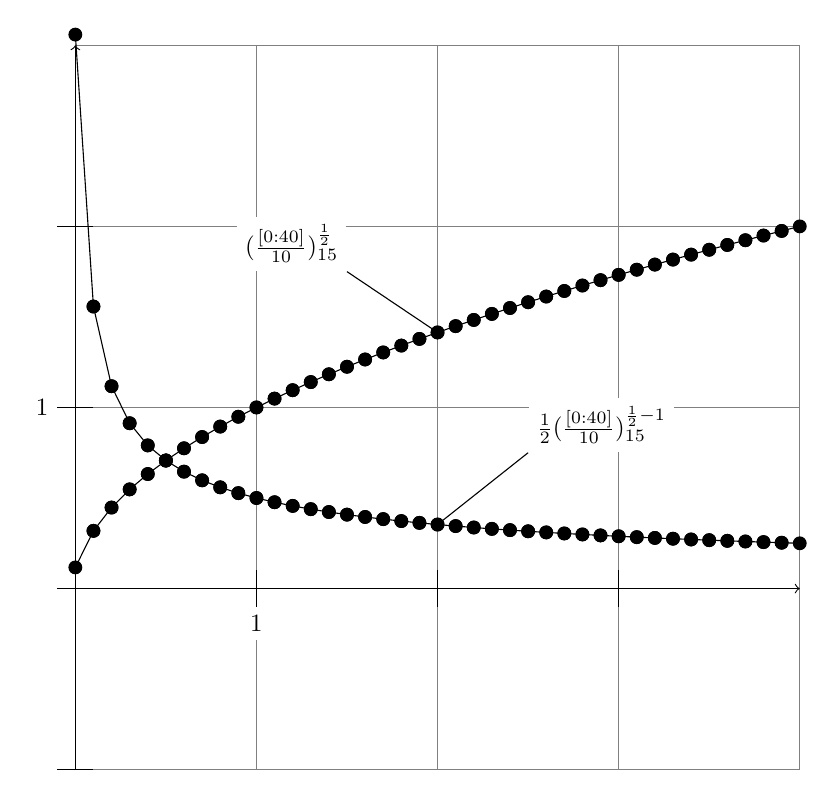
\begin{tikzpicture}[scale=2.3,every node/.style={scale=0.9}]
            \draw[step=1,help lines] (0.000000,-1.000000) grid (4.000000,3.000000);
            \draw[->] (0.000000,0) -- (4.000000,0);
            \draw[->] (0,-1.000000) -- (0,3.000000);
            \draw (0.000000, 0.100000) -- (0.000000,-0.100000);
            \draw (1.000000, 0.100000) -- (1.000000,-0.100000);
            \draw (2.000000, 0.100000) -- (2.000000,-0.100000);
            \draw (3.000000, 0.100000) -- (3.000000,-0.100000);
            \draw (0.100000, -1.000000) -- (-0.100000,-1.000000);
            \draw (0.100000, 0.000000) -- (-0.100000,0.000000);
            \draw (0.100000, 1.000000) -- (-0.100000,1.000000);
            \draw (0.100000, 2.000000) -- (-0.100000,2.000000);
            \draw (1,-0.100000) node[anchor=north,fill=white]{$1$};
            \draw (-0.100000,1) node[anchor=east,fill=white]{$1$};
            \draw (2.5,0.75) node[anchor=south west,fill=white]{$\frac{1}{2}(\frac{[0:40]}{10})_{15}^{\frac{1}{2}-1}$};
            \draw (2,0.35355339059327373) -- (2.5,0.75);
            \draw (1.5,1.75) node[anchor=south east,fill=white]{$(\frac{[0:40]}{10})_{15}^{\frac{1}{2}}$};
            \draw (2,1.4142135623730951) -- (1.5,1.75);
            \filldraw (0.000000,0.116646) circle (1pt);
            \draw (0.000000,0.116646) -- (0.100000,0.318661);
            \filldraw (0.100000,0.318661) circle (1pt);
            \filldraw (0.000000,3.058883) circle (1pt);
            \draw (0.000000,3.058883) -- (0.100000,1.557337);
            \filldraw (0.100000,1.557337) circle (1pt);
            \filldraw (0.100000,0.318661) circle (1pt);
            \draw (0.100000,0.318661) -- (0.200000,0.447352);
            \filldraw (0.200000,0.447352) circle (1pt);
            \filldraw (0.100000,1.557337) circle (1pt);
            \draw (0.100000,1.557337) -- (0.200000,1.117423);
            \filldraw (0.200000,1.117423) circle (1pt);
            \filldraw (0.200000,0.447352) circle (1pt);
            \draw (0.200000,0.447352) -- (0.300000,0.547729);
            \filldraw (0.300000,0.547729) circle (1pt);
            \filldraw (0.200000,1.117423) circle (1pt);
            \draw (0.200000,1.117423) -- (0.300000,0.912853);
            \filldraw (0.300000,0.912853) circle (1pt);
            \filldraw (0.300000,0.547729) circle (1pt);
            \draw (0.300000,0.547729) -- (0.400000,0.632456);
            \filldraw (0.400000,0.632456) circle (1pt);
            \filldraw (0.300000,0.912853) circle (1pt);
            \draw (0.300000,0.912853) -- (0.400000,0.790569);
            \filldraw (0.400000,0.790569) circle (1pt);
            \filldraw (0.400000,0.632456) circle (1pt);
            \draw (0.400000,0.632456) -- (0.500000,0.707107);
            \filldraw (0.500000,0.707107) circle (1pt);
            \filldraw (0.400000,0.790569) circle (1pt);
            \draw (0.400000,0.790569) -- (0.500000,0.707107);
            \filldraw (0.500000,0.707107) circle (1pt);
            \filldraw (0.500000,0.707107) circle (1pt);
            \draw (0.500000,0.707107) -- (0.600000,0.774597);
            \filldraw (0.600000,0.774597) circle (1pt);
            \filldraw (0.500000,0.707107) circle (1pt);
            \draw (0.500000,0.707107) -- (0.600000,0.645497);
            \filldraw (0.600000,0.645497) circle (1pt);
            \filldraw (0.600000,0.774597) circle (1pt);
            \draw (0.600000,0.774597) -- (0.700000,0.836660);
            \filldraw (0.700000,0.836660) circle (1pt);
            \filldraw (0.600000,0.645497) circle (1pt);
            \draw (0.600000,0.645497) -- (0.700000,0.597614);
            \filldraw (0.700000,0.597614) circle (1pt);
            \filldraw (0.700000,0.836660) circle (1pt);
            \draw (0.700000,0.836660) -- (0.800000,0.894427);
            \filldraw (0.800000,0.894427) circle (1pt);
            \filldraw (0.700000,0.597614) circle (1pt);
            \draw (0.700000,0.597614) -- (0.800000,0.559017);
            \filldraw (0.800000,0.559017) circle (1pt);
            \filldraw (0.800000,0.894427) circle (1pt);
            \draw (0.800000,0.894427) -- (0.900000,0.948683);
            \filldraw (0.900000,0.948683) circle (1pt);
            \filldraw (0.800000,0.559017) circle (1pt);
            \draw (0.800000,0.559017) -- (0.900000,0.527046);
            \filldraw (0.900000,0.527046) circle (1pt);
            \filldraw (0.900000,0.948683) circle (1pt);
            \draw (0.900000,0.948683) -- (1.000000,1.000000);
            \filldraw (1.000000,1.000000) circle (1pt);
            \filldraw (0.900000,0.527046) circle (1pt);
            \draw (0.900000,0.527046) -- (1.000000,0.500000);
            \filldraw (1.000000,0.500000) circle (1pt);
            \filldraw (1.000000,1.000000) circle (1pt);
            \draw (1.000000,1.000000) -- (1.100000,1.048809);
            \filldraw (1.100000,1.048809) circle (1pt);
            \filldraw (1.000000,0.500000) circle (1pt);
            \draw (1.000000,0.500000) -- (1.100000,0.476731);
            \filldraw (1.100000,0.476731) circle (1pt);
            \filldraw (1.100000,1.048809) circle (1pt);
            \draw (1.100000,1.048809) -- (1.200000,1.095445);
            \filldraw (1.200000,1.095445) circle (1pt);
            \filldraw (1.100000,0.476731) circle (1pt);
            \draw (1.100000,0.476731) -- (1.200000,0.456435);
            \filldraw (1.200000,0.456435) circle (1pt);
            \filldraw (1.200000,1.095445) circle (1pt);
            \draw (1.200000,1.095445) -- (1.300000,1.140175);
            \filldraw (1.300000,1.140175) circle (1pt);
            \filldraw (1.200000,0.456435) circle (1pt);
            \draw (1.200000,0.456435) -- (1.300000,0.438529);
            \filldraw (1.300000,0.438529) circle (1pt);
            \filldraw (1.300000,1.140175) circle (1pt);
            \draw (1.300000,1.140175) -- (1.400000,1.183216);
            \filldraw (1.400000,1.183216) circle (1pt);
            \filldraw (1.300000,0.438529) circle (1pt);
            \draw (1.300000,0.438529) -- (1.400000,0.422577);
            \filldraw (1.400000,0.422577) circle (1pt);
            \filldraw (1.400000,1.183216) circle (1pt);
            \draw (1.400000,1.183216) -- (1.500000,1.224745);
            \filldraw (1.500000,1.224745) circle (1pt);
            \filldraw (1.400000,0.422577) circle (1pt);
            \draw (1.400000,0.422577) -- (1.500000,0.408248);
            \filldraw (1.500000,0.408248) circle (1pt);
            \filldraw (1.500000,1.224745) circle (1pt);
            \draw (1.500000,1.224745) -- (1.600000,1.264911);
            \filldraw (1.600000,1.264911) circle (1pt);
            \filldraw (1.500000,0.408248) circle (1pt);
            \draw (1.500000,0.408248) -- (1.600000,0.395285);
            \filldraw (1.600000,0.395285) circle (1pt);
            \filldraw (1.600000,1.264911) circle (1pt);
            \draw (1.600000,1.264911) -- (1.700000,1.303840);
            \filldraw (1.700000,1.303840) circle (1pt);
            \filldraw (1.600000,0.395285) circle (1pt);
            \draw (1.600000,0.395285) -- (1.700000,0.383482);
            \filldraw (1.700000,0.383482) circle (1pt);
            \filldraw (1.700000,1.303840) circle (1pt);
            \draw (1.700000,1.303840) -- (1.800000,1.341641);
            \filldraw (1.800000,1.341641) circle (1pt);
            \filldraw (1.700000,0.383482) circle (1pt);
            \draw (1.700000,0.383482) -- (1.800000,0.372678);
            \filldraw (1.800000,0.372678) circle (1pt);
            \filldraw (1.800000,1.341641) circle (1pt);
            \draw (1.800000,1.341641) -- (1.900000,1.378405);
            \filldraw (1.900000,1.378405) circle (1pt);
            \filldraw (1.800000,0.372678) circle (1pt);
            \draw (1.800000,0.372678) -- (1.900000,0.362738);
            \filldraw (1.900000,0.362738) circle (1pt);
            \filldraw (1.900000,1.378405) circle (1pt);
            \draw (1.900000,1.378405) -- (2.000000,1.414214);
            \filldraw (2.000000,1.414214) circle (1pt);
            \filldraw (1.900000,0.362738) circle (1pt);
            \draw (1.900000,0.362738) -- (2.000000,0.353553);
            \filldraw (2.000000,0.353553) circle (1pt);
            \filldraw (2.000000,1.414214) circle (1pt);
            \draw (2.000000,1.414214) -- (2.100000,1.449138);
            \filldraw (2.100000,1.449138) circle (1pt);
            \filldraw (2.000000,0.353553) circle (1pt);
            \draw (2.000000,0.353553) -- (2.100000,0.345033);
            \filldraw (2.100000,0.345033) circle (1pt);
            \filldraw (2.100000,1.449138) circle (1pt);
            \draw (2.100000,1.449138) -- (2.200000,1.483240);
            \filldraw (2.200000,1.483240) circle (1pt);
            \filldraw (2.100000,0.345033) circle (1pt);
            \draw (2.100000,0.345033) -- (2.200000,0.337100);
            \filldraw (2.200000,0.337100) circle (1pt);
            \filldraw (2.200000,1.483240) circle (1pt);
            \draw (2.200000,1.483240) -- (2.300000,1.516575);
            \filldraw (2.300000,1.516575) circle (1pt);
            \filldraw (2.200000,0.337100) circle (1pt);
            \draw (2.200000,0.337100) -- (2.300000,0.329690);
            \filldraw (2.300000,0.329690) circle (1pt);
            \filldraw (2.300000,1.516575) circle (1pt);
            \draw (2.300000,1.516575) -- (2.400000,1.549193);
            \filldraw (2.400000,1.549193) circle (1pt);
            \filldraw (2.300000,0.329690) circle (1pt);
            \draw (2.300000,0.329690) -- (2.400000,0.322749);
            \filldraw (2.400000,0.322749) circle (1pt);
            \filldraw (2.400000,1.549193) circle (1pt);
            \draw (2.400000,1.549193) -- (2.500000,1.581138);
            \filldraw (2.500000,1.581138) circle (1pt);
            \filldraw (2.400000,0.322749) circle (1pt);
            \draw (2.400000,0.322749) -- (2.500000,0.316228);
            \filldraw (2.500000,0.316228) circle (1pt);
            \filldraw (2.500000,1.581138) circle (1pt);
            \draw (2.500000,1.581138) -- (2.600000,1.612450);
            \filldraw (2.600000,1.612450) circle (1pt);
            \filldraw (2.500000,0.316228) circle (1pt);
            \draw (2.500000,0.316228) -- (2.600000,0.310087);
            \filldraw (2.600000,0.310087) circle (1pt);
            \filldraw (2.600000,1.612450) circle (1pt);
            \draw (2.600000,1.612450) -- (2.700000,1.643165);
            \filldraw (2.700000,1.643165) circle (1pt);
            \filldraw (2.600000,0.310087) circle (1pt);
            \draw (2.600000,0.310087) -- (2.700000,0.304291);
            \filldraw (2.700000,0.304291) circle (1pt);
            \filldraw (2.700000,1.643165) circle (1pt);
            \draw (2.700000,1.643165) -- (2.800000,1.673316);
            \filldraw (2.800000,1.673316) circle (1pt);
            \filldraw (2.700000,0.304291) circle (1pt);
            \draw (2.700000,0.304291) -- (2.800000,0.298808);
            \filldraw (2.800000,0.298808) circle (1pt);
            \filldraw (2.800000,1.673316) circle (1pt);
            \draw (2.800000,1.673316) -- (2.900000,1.702932);
            \filldraw (2.900000,1.702932) circle (1pt);
            \filldraw (2.800000,0.298808) circle (1pt);
            \draw (2.800000,0.298808) -- (2.900000,0.293611);
            \filldraw (2.900000,0.293611) circle (1pt);
            \filldraw (2.900000,1.702932) circle (1pt);
            \draw (2.900000,1.702932) -- (3.000000,1.732040);
            \filldraw (3.000000,1.732040) circle (1pt);
            \filldraw (2.900000,0.293611) circle (1pt);
            \draw (2.900000,0.293611) -- (3.000000,0.288676);
            \filldraw (3.000000,0.288676) circle (1pt);
            \filldraw (3.000000,1.732040) circle (1pt);
            \draw (3.000000,1.732040) -- (3.100000,1.760666);
            \filldraw (3.100000,1.760666) circle (1pt);
            \filldraw (3.000000,0.288676) circle (1pt);
            \draw (3.000000,0.288676) -- (3.100000,0.283983);
            \filldraw (3.100000,0.283983) circle (1pt);
            \filldraw (3.100000,1.760666) circle (1pt);
            \draw (3.100000,1.760666) -- (3.200000,1.788832);
            \filldraw (3.200000,1.788832) circle (1pt);
            \filldraw (3.100000,0.283983) circle (1pt);
            \draw (3.100000,0.283983) -- (3.200000,0.279511);
            \filldraw (3.200000,0.279511) circle (1pt);
            \filldraw (3.200000,1.788832) circle (1pt);
            \draw (3.200000,1.788832) -- (3.300000,1.816559);
            \filldraw (3.300000,1.816559) circle (1pt);
            \filldraw (3.200000,0.279511) circle (1pt);
            \draw (3.200000,0.279511) -- (3.300000,0.275244);
            \filldraw (3.300000,0.275244) circle (1pt);
            \filldraw (3.300000,1.816559) circle (1pt);
            \draw (3.300000,1.816559) -- (3.400000,1.843865);
            \filldraw (3.400000,1.843865) circle (1pt);
            \filldraw (3.300000,0.275244) circle (1pt);
            \draw (3.300000,0.275244) -- (3.400000,0.271167);
            \filldraw (3.400000,0.271167) circle (1pt);
            \filldraw (3.400000,1.843865) circle (1pt);
            \draw (3.400000,1.843865) -- (3.500000,1.870770);
            \filldraw (3.500000,1.870770) circle (1pt);
            \filldraw (3.400000,0.271167) circle (1pt);
            \draw (3.400000,0.271167) -- (3.500000,0.267266);
            \filldraw (3.500000,0.267266) circle (1pt);
            \filldraw (3.500000,1.870770) circle (1pt);
            \draw (3.500000,1.870770) -- (3.600000,1.897289);
            \filldraw (3.600000,1.897289) circle (1pt);
            \filldraw (3.500000,0.267266) circle (1pt);
            \draw (3.500000,0.267266) -- (3.600000,0.263530);
            \filldraw (3.600000,0.263530) circle (1pt);
            \filldraw (3.600000,1.897289) circle (1pt);
            \draw (3.600000,1.897289) -- (3.700000,1.923437);
            \filldraw (3.700000,1.923437) circle (1pt);
            \filldraw (3.600000,0.263530) circle (1pt);
            \draw (3.600000,0.263530) -- (3.700000,0.259946);
            \filldraw (3.700000,0.259946) circle (1pt);
            \filldraw (3.700000,1.923437) circle (1pt);
            \draw (3.700000,1.923437) -- (3.800000,1.949228);
            \filldraw (3.800000,1.949228) circle (1pt);
            \filldraw (3.700000,0.259946) circle (1pt);
            \draw (3.700000,0.259946) -- (3.800000,0.256505);
            \filldraw (3.800000,0.256505) circle (1pt);
            \filldraw (3.800000,1.949228) circle (1pt);
            \draw (3.800000,1.949228) -- (3.900000,1.974676);
            \filldraw (3.900000,1.974676) circle (1pt);
            \filldraw (3.800000,0.256505) circle (1pt);
            \draw (3.800000,0.256505) -- (3.900000,0.253198);
            \filldraw (3.900000,0.253198) circle (1pt);
            \filldraw (3.900000,1.974676) circle (1pt);
            \draw (3.900000,1.974676) -- (4.000000,1.999792);
            \filldraw (4.000000,1.999792) circle (1pt);
            \filldraw (3.900000,0.253198) circle (1pt);
            \draw (3.900000,0.253198) -- (4.000000,0.250016);
            \filldraw (4.000000,0.250016) circle (1pt);
			    \end{tikzpicture}
		    \end{minipage}
		    \begin{minipage}[c]{0.35\textwidth}
			    A plot of the lists of complex numbers $(\frac{[0:40]}{10})_{15}^{\frac{1}{2}}$ and $\frac{1}{2}(\frac{[0:40]}{10})_{15}^{\frac{1}{2}-1}$. Note that the steepness of $(\frac{[0:40]}{10})_{15}^{\frac{1}{2}}$ is approximately given by the y-coordinates of $\frac{1}{2}(\frac{[0:40]}{10})_{15}^{\frac{1}{2}-1}$. That is, where the graph of $(\frac{[0:40]}{10})_{15}^{\frac{1}{2}}$ is rapidly increasing, the graph of $\frac{1}{2}(\frac{[0:40]}{10})_{15}^{\frac{1}{2}-1}$ has a relatively large positive value, and where the graph of $(\frac{[0:40]}{10})_{15}^{\frac{1}{2}}$ flattens out, the graph of $\frac{1}{2}(\frac{[0:40]}{10})_{15}^{\frac{1}{2}-1}$ has a relatively small positive value.
		    \end{minipage}
	  \chapter{Integral Arithmetic}
	    \begin{multicols*}{2}
	      \declaration{3.30}
			    The notation \gls{differentialintegral}, where:
			    \begin{enumerate}
			      \item $f(r,\delta_r)$ is a procedure to construct a complex number when complex numbers $r,\delta_r$ such that $P(r,\delta_r)$ are chosen
			      \item $R$ is a non-empty list of complex numbers such that $P(R_t,R_{t+1}-R_t)$ for $t\in[0:\lvert R\rvert-1]$
			    \end{enumerate}
			    will be used as a shorthand for $\sum_t^{[0:\lvert R\rvert-1]}f(R_t,R_{t+1}-R_{t})$.
		    \procedure{3.86}
			    \objective
				    Choose the following:
				    \begin{enumerate}
				      \item A procedure $f(r,\delta)$ to construct a complex number when complex numbers $r,\delta_r$ such that $P(r,\delta_r)$ are chosen.
				      \item A procedure $g(r,\delta)$ to construct a complex number when complex numbers $r,\delta_r$ such that $Q(r,\delta_r)$ are chosen.
				      \item A non-empty list of complex numbers $R$ such that $P(R_t,R_{t+1}-R_t)$ and $Q(R_t,R_{t+1}-R_t)$ for $t\in[0:\lvert R\rvert-1]$.
				    \end{enumerate}
				    The objective of the following instructions is to show that $\int_r^R(f(r,\delta_r)+g(r,\delta_r))=\int_r^Rf(r,\delta_r)+\int_r^Rg(r,\delta_r)$.
			    \implementation
				    \begin{enumerate}
					    \item Verify that $\int_r^R(f(r,\delta_r)+g(r,\delta_r))$
					    \begin{enumerate}
						    \item $=\sum_t^{[0:\lvert R\rvert-1]}(f(R_t,R_{t+1}-R_t)+g(R_t,R_{t+1}-R_t))$
						    \item $=\sum_t^{[0:\lvert R\rvert-1]}f(R_t,R_{t+1}-R_t)+\sum_t^{[0:\lvert R\rvert-1]}g(R_t,R_{t+1}-R_t)$
						    \item $=\int_r^Rf(r,\delta_r)+\int_r^Rg(r,\delta_r)$
					    \end{enumerate}
				    \end{enumerate}
		    \procedure{3.87}
			    \objective
				    Choose the following:
				    \begin{enumerate}
				      \item A complex number $a$.
				      \item A procedure $f(r,\delta)$ to construct a complex number when complex numbers $r,\delta_r$ such that $P(r,\delta_r)$ are chosen.
				      \item A non-empty list of complex numbers $R$ such that $P(R_t, R_{t+1}-R_t)$ for $t\in[0:\lvert R\rvert-1]$.
				    \end{enumerate}
				     The objective of the following instructions is to show that $\int_r^Raf(r,\delta_r)=a\int_r^Rf(r,\delta_r)$.
			    \implementation
				    \begin{enumerate}
					    \item Verify that $\int_r^Raf(r,\delta_r)$
					    \begin{enumerate}
						    \item $=\sum_t^{[0:\lvert R\rvert-1]}af(R_t,R_{t+1}-R_t)$
						    \item $=a\sum_t^{[0:\lvert R\rvert-1]}f(R_t,R_{t+1}-R_t)$
						    \item $=a\int_r^Rf(r,\delta_r)$
					    \end{enumerate}
				    \end{enumerate}
		    \procedure{3.88}
			    \objective
				    Choose the following:
				    \begin{enumerate}
				      \item A procedure $f(r)$ to construct a complex number when a complex number $r$ such that $P(r)$ is chosen.
				      \item A non-empty list of complex numbers $R$ such that $P(R_t)$ for $t\in[0:\lvert R\rvert-1]$.
				      \item A non-empty list of complex numbers $S$ such that $P(S_t)$ for $t\in[0:\lvert R\rvert-1]$ and $R_{\lvert R\rvert-1}=S_0$.
				    \end{enumerate}
				    The objective of the following instructions is to show that $\int_r^{R^\frown S}f(r)\delta_r=\int_r^Rf(r)\delta_r+\int_r^Sf(r)\delta_r$.
			    \implementation
				    \begin{enumerate}
					    \item Let $T=R^\frown S$.
					    \item Verify that $\int_r^{T}f(r)\delta_r$
					    \begin{enumerate}
						    \item $=\sum_t^{[0:\lvert T\rvert-1]}f(T_t)(T_{t+1}-T_t)$
						    \item $=\sum_t^{[0:\lvert R\rvert-1]}f(T_t)(T_{t+1}-T_t)+\sum_t^{[\lvert R\rvert-1:\lvert R\rvert]}f(T_t)(T_{t+1}-T_t)+\sum_t^{[\lvert R\rvert:\lvert T\rvert-1]}f(T_t)(T_{t+1}-T_t)$
						    \item $=\sum_t^{[0:\lvert R\rvert-1]}f(R_t)(R_{t+1}-R_t)+f(T_{\lvert R\rvert-1})(T_{\lvert R\rvert}-T_{\lvert R\rvert-1})+\sum_t^{[\lvert R\rvert:\lvert T\rvert-1]}f(S_{t-\lvert R\rvert})\cdot(S_{t+1-\lvert R\rvert}-S_{t-\lvert R\rvert})$
						    \item $=\sum_t^{[0:\lvert R\rvert-1]}f(R_t)(R_{t+1}-R_t)+f(T_{\lvert R\rvert-1})(S_0-R_{\lvert R\rvert-1})+\sum_t^{[0:\lvert S\rvert-1]}f(S_{t})(S_{t+1}-S_{t})$
						    \item $=\int_r^Rf(r)\delta_r+\int_r^Sf(r)\delta_r$.
					    \end{enumerate}
				    \end{enumerate}
		    \procedure{3.34}
			    \objective
				    Choose the following:
				    \begin{enumerate}
				      \item A procedure $f(r)$ to construct a complex number when a complex number $r$ such that $P(r)$ is chosen.
				      \item A non-empty list of complex numbers $R$ such that $P(R_t)$ for $t\in[0:\lvert R\rvert-1]$.
				    \end{enumerate}
				    The objective of the following instructions is to show that $\int_r^R\delta_r\diff_{z=r}^{+\delta_r}f(z)=f(R_{\lvert R\rvert-1})-f(R_0)$.
			    \implementation
				    \begin{enumerate}
					    \item Verify that $\int_r^R\delta_r\diff_{z=r}^{\delta_r}f(z)$
					    \begin{enumerate}
						    \item $=\int_r^R\delta_r(\frac{f(r+\delta_r)-f(r)}{\delta_r})$
						    \item $=\int_r^R(f(r+\delta_r)-f(r))$
						    \item $=\sum_k^{[0:\lvert R\rvert-1]}(f(R_{k+1})-f(R_k))$
						    \item $=f(R_{\lvert R\rvert-1})-f(R_0)$.
					    \end{enumerate}
				    \end{enumerate}
		    \declaration{3.31}
			    The notation \gls{differentialDeltaX}, where $X$ is a list, will be used as a shorthand for $\langle X_1-X_0,X_2-X_1,\cdots,X_{\lvert X\rvert-1}-X_{\lvert X\rvert-2}\rangle$.
		    \procedure{fri3008190328}
		      \objective
		        Choose the following:
		        \begin{enumerate}
		          \item A non-negative rational number $A$.
				      \item A procedure $q_1(x,n,\delta)$ to show that $\Delta_{y=x}^{+\delta}f_n(y)\equiv f'_n(x)\err{\frac{a_1}{n}+b_1\{\delta\}}$ when two complex numbers $x,\delta$ and a positive integer $n$ such that $P(x)$, $n>c_1$, and $0<\lVert\delta\rVert^2<{d_1}^2$ are chosen.
				    \end{enumerate}
				    The objective of the following instructions is to construct the following:
				    \begin{enumerate}
				      \item Non-negative rational numbers $a,b,c,d$.
				      \item A procedure $p(R,n)$ to show that $\int_r^Rf'_n(r)\delta_r\equiv f_n(R_{\lvert R\rvert-1})-f_n(R_0)\err{\frac{a}{n}+b\max(\{\Delta R\})}$ when an integer $n$ and a non-empty list of complex numbers $R$ such that $P(R_t)$ and $0<\lVert R_{t+1}-R_t\rVert^2<{d}^2$ for $t\in[0:\lvert R\rvert-1]$, $\int_r^R\{\delta_r\}\le A$, and $n>c$ are chosen.
				    \end{enumerate}
		      \implementation
		        \begin{enumerate}
		          \item Let $a=a_1A$.
		          \item Let $b=b_1A$.
		          \item Let $c=c_1$.
		          \item Let $d=d_1$.
		          \item Let $p(R,n)$ be the following procedure:
		          \begin{enumerate}
		            \item Using procedure $q_1$, verify that $\int_r^Rf'_n(r)\delta_r$
		            \begin{enumerate}
		              \item $=\sum_k^{[0:\lvert R\rvert-1]}f'_n(R_k)(R_{k+1}-R_k)$
		              \item $\equiv\sum_k^{0:\lvert R\rvert-1}\Delta_{y=R_k}^{R_{k+1}-R_k}f_n(y)(R_{k+1}-R_k)$
		              \begin{enumerate}
		                \item $\err{\sum_k^{0:\lvert R\rvert-1}(\frac{a_1}{n}+b_1\{R_{k+1}-R_k\})\{R_{k+1}-R_k\}}$
		                \item $\err{(\frac{a_1}{n}+b_1\max(\{\Delta R\}))\sum_k^{0:\lvert R\rvert-1}\{R_{k+1}-R_k\}}$
		                \item $\err{(\frac{a_1}{n}+b_1\max(\{\Delta R\}))\int_r^R\{\delta_r\}}$
		                \item $\err{(\frac{a_1}{n}+b_1\max(\{\Delta R\}))A}$
		                \item $\err{\frac{a}{n}+b\max(\{\Delta R\})}$
		              \end{enumerate}
		              \item $=\sum_k^{0:\lvert R\rvert-1}\frac{f_n(R_k+(R_{k+1}-R_k))-f_n(R_k)}{R_{k+1}-R_k}\cdot(R_{k+1}-R_k)$
		              \item $=\sum_k^{0:\lvert R\rvert-1}(f_n(R_{k+1})-f_n(R_k))$
		              \item $=f_n(R_{\lvert R\rvert-1})-f_n(R_0)$.
		            \end{enumerate}
		            \item \textbf{Therefore verify that $\int_r^Rf'_n(r)\delta_r\equiv f_n(R_{\lvert R\rvert-1})-f_n(R_0)\err{\frac{a}{n}+b\max(\{\Delta R\})}$.}
		          \end{enumerate}
		          \item \textbf{Yield the tuple $\langle a,b,c,d,p\rangle$.}
		        \end{enumerate}
		    \procedure{fri3008190457}
		      \objective
		        Choose the following:
		        \begin{enumerate}
		          \item A non-negative rational number $A$.
				      \item A procedure $q_1(x,n,\delta)$ to show that $\Delta_{y=x}^{+\delta}g_n(y)\equiv g'_n(x)\err{\frac{a_1}{n}+b_1\{\delta\}}$ when two complex numbers $x,\delta$ and a positive integer $n$ such that $P(x)$, $n>c_1$, and $0<\lVert\delta\rVert^2<{d_1}^2$ are chosen.
				      \item A procedure $q_2(x,n)$ to show that $f_n(x)\equiv 0\err{a_2}$ when a complex number $x$ and a positive integer $n$ such that $Q(x)$ and $n>b_2$ are chosen.
				      \item A procedure $q_3(x,n)$ to show that $Q(g_n(x))$ when a complex number $x$ and a positive integer $n$ such that $P(x)$ and $n>c_1$ are chosen
				    \end{enumerate}
				    The objective of the following instructions is to construct the following:
				    \begin{enumerate}
				      \item Non-negative rational numbers $a,b,c,d$.
				      \item A procedure $p(R,n)$ to show that $\int_r^{g(R)}f_n(r)\delta_r\equiv\int_r^Rf_n(g_n(r))g'_n(r)\delta_r\err{\frac{a}{n}+b\max(\{\Delta R\})}$ when an integer $n$ and a non-empty list of complex numbers $R$ such that $P(R_t)$ and $0<\lVert R_{t+1}-R_t\rVert^2<{d}^2$ for $t\in[0:\lvert R\rvert-1]$, $\int_r^R\{\delta_r\}\le A$, and $n>c$ are chosen.
				    \end{enumerate}
			    \implementation
			      \begin{enumerate}
			        \item Let $a=a_1a_2A$.
			        \item Let $b=b_1a_2A$.
			        \item Let $c=\max(c_1,b_2)$.
			        \item Let $d=d_1$.
			        \item Let $p(R,n)$ be the following procedure:
			        \begin{enumerate}
			          \item Using procedures $q_1,q_2,q_3$, verify that $\int_r^{g_n(R)}f_n(r)\delta_r$
			          \begin{enumerate}
			            \item $=\sum_k^{[0:\lvert R\rvert-1]}f_n(g_n(R_k))(g_n(R_{k+1})-g_n(R_k))$
			            \item $=\sum_k^{[0:\lvert R\rvert-1]}f_n(g_n(R_k))\Delta_{y=R_k}^{R_{k+1}-R_k}g_n(y)(R_{k+1}-R_k)$
			            \item $\equiv\sum_k^{[0:\lvert R\rvert-1]}f_n(g_n(R_k))g'_n(R_k)(R_{k+1}-R_k)$
			            \begin{enumerate}
			              \item $\err{\sum_k^{[0:\lvert R\rvert-1]}a_2(\frac{a_1}{n}+b_1\{R_{k+1}-R_k\})\{R_{k+1}-R_k\}}$
			              \item $\err{a_2(\frac{a_1}{n}+b_1\max(\{\Delta R\}))\sum_k^{[0:\lvert R\rvert-1]}\{R_{k+1}-R_k\}}$
			              \item $\err{a_2(\frac{a_1}{n}+b_1\max(\{\Delta R\}))\int_r^R\{\delta_r\}}$
			              \item $\err{a_2(\frac{a_1}{n}+b_1\max(\{\Delta R\}))A}$
			              \item $\err{\frac{a}{n}+b\max(\{\Delta R\})}$
			            \end{enumerate}
			            \item $=\int_r^Rf_n(g_n(r))g'_n(r)\delta_r$.
			          \end{enumerate}
			          \item \textbf{Hence verify that $\int_r^{g_n(R)}f_n(r)\delta_r\equiv\int_r^Rf_n(g_n(r))g'_n(r)\delta_r\err{\frac{a}{n}+b\max(\{\Delta R\})}$.}
			        \end{enumerate}
			        \item \textbf{Yield the tuple $\langle a,b,c,d,p\rangle$.}
			      \end{enumerate}
		    \procedure{fri3008190709}
		      \objective
		        Choose three rational numbers $A,X,\epsilon$ such that $0<\epsilon<1$ and $X\ge 0$. The objective of the following instructions is to construct the following:
				    \begin{enumerate}
				      \item Non-negative rational numbers $a,b,c,d$.
				      \item A procedure $p(R,n)$ to show that $\int_r^R\frac{\delta_r}{r}\equiv\ln_n(R_{\lvert R\rvert-1})\err{\frac{a}{n}+b\max(\{\Delta R\})}$ when an integer $n$ and a non-empty list of complex numbers $R$ such that $\Re(R_t)\ge\epsilon$, $\lVert R_t\rVert^2\le X^2$ and $0<\lVert R_{t+1}-R_t\rVert^2<{d}^2$ for $t\in[0:\lvert R\rvert-1]$, $R_0=1$, $\int_r^R\{\delta_r\}\le A$, and $n>c$ are chosen.
				    \end{enumerate}
		      \implementation
		        \begin{enumerate}
		          \item Execute \procedurehr{wed2108191603} on $\langle X,\epsilon\rangle$ and let $\langle\cdots,q\rangle$ receive.
		          \item Hence execute \procedurehr{fri3008190328} on $\langle A,q\rangle$ and let $\langle a,b,c,d,t\rangle$ receive.
		          \item Let $p(R,n)$ be the following procedure:
		          \begin{enumerate}
		            \item Using procedure $t$, verify that $\int_r^R\frac{\delta_r}{r}$
		            \begin{enumerate}
		              \item $\equiv\ln_n(R_{\lvert R\rvert-1})-\ln_n(R_0)\err{\frac{a}{n}+b\max(\{\Delta R\})}$
		              \item $=\ln_n(R_{\lvert R\rvert-1})-\ln_n(1)$
		              \item $=\ln_n(R_{\lvert R\rvert-1})$.
		            \end{enumerate}
		            \item \textbf{Hence verify that $\int_r^R\frac{\delta_r}{r}\equiv\ln_n(R_{\lvert R\rvert-1})\err{\frac{a}{n}+b\max(\{\Delta R\})}$.}
		          \end{enumerate}
		          \item \textbf{Yield the tuple $\langle a,b,c,d,p\rangle$.}
		        \end{enumerate}
	    \end{multicols*}
	  \clearpage
	\part{Matrix Arithmetic}
	  \chapter{Matrix Arithmetic}
	    \begin{multicols*}{2}
		    \declaration{4.28}
			    The phrase "\gls{matrix}" will be used as a shorthand for a list of equally lengthed lists of polynomials. In particular, the phrase "$m\times n$ matrix" will be used as a shorthand for a length-$m$ list of length-$n$ lists of polynomials.
		    \declaration{4.29}
			    The notation \gls{matrixentry}, where $A$ is a matrix and $I,J$ are lists of indicies, will be used as a shorthand for $\langle(A_j)_J\for j\in I\rangle$.
		    \declaration{4.30}
			    The phrase "\gls{matrixA=B}", where $A,B$ are $m\times n$ matrices, will be used as a shorthand for "$A_{i,j}=B_{i,j}$ for $j\in[0:n]$, for $i\in[0:m]$".
		    \procedure{4.73}
			    \objective
				    Choose an $m\times n$ matrix $A$. The objective of the following instructions is to show that $A=A$.
			    \implementation
				    \begin{enumerate}
					    \item Verify that $A_{i,j}=A_{i,j}$ for $j\in[0:n]$, for $i\in[0:m]$.
					    \item \textbf{Hence verify that $A=A$.}
				    \end{enumerate}
		    \procedure{4.74}
			    \objective
				    Choose two $m\times n$ matrices $A,B$ such that $A=B$. The objective of the following instructions is to show that $B=A$.
			    \implementation
				    \begin{enumerate}
					    \item Verify that $A_{i,j}=B_{i,j}$ for $j\in[0:n]$, for $i\in[0:m]$.
					    \item Hence verify that $B_{i,j}=A_{i,j}$ for $j\in[0:n]$, for $i\in[0:m]$.
					    \item \textbf{Hence verify that $B=A$.}
				    \end{enumerate}
		    \procedure{4.75}
			    \objective
				    Choose three $m\times n$ matrices $A,B,C$ such that $A=B$ and $B=C$. The objective of the following instructions is to show that $A=C$.
			    \implementation
				    \begin{enumerate}
					    \item Verify that $A_{i,j}=B_{i,j}$ for $j\in[0:n]$, for $i\in[0:m]$.
					    \item Verify that $B_{i,j}=C_{i,j}$ for $j\in[0:n]$, for $i\in[0:m]$.
					    \item Hence verify that $A_{i,j}=C_{i,j}$ for $j\in[0:n]$, for $i\in[0:m]$.
					    \item \textbf{Hence verify that $A=C$.}
				    \end{enumerate}
		    \declaration{4.31}
			    The notation \gls{matrixA+B}, where $A,B$ are $m\times n$ matrices, will be used as a shorthand for the list $\langle\langle A_{i,j}+B_{i,j}\for j\in[0:n]\rangle\for i\in[0:m]\rangle$.
		    \procedure{4.76}
			    \objective
				    Choose four $m\times n$ matrices $A,B,C,D$ such that $A=C$ and $B=D$. The objective of the following instructions is to show that $A+B=C+D$.
			    \implementation
				    \begin{enumerate}
					    \item Verify that $A_{i,j}=C_{i,j}$ for $j\in[0:n]$, for $i\in[0:m]$.
					    \item Verify that $B_{i,j}=D_{i,j}$ for $j\in[0:n]$, for $i\in[0:m]$.
					    \item Hence verify that $A+B$
					    \begin{enumerate}
						    \item $=\langle\langle A_{i,j}+B_{i,j}\for j\in[0:n]\rangle\for i\in[0:m]\rangle$
						    \item $=\langle\langle C_{i,j}+D_{i,j}\for j\in[0:n]\rangle\for i\in[0:m]\rangle$
						    \item $=C+D$.
					    \end{enumerate}
				    \end{enumerate}
		    \procedure{4.77}
			    \objective
				    Choose three $m\times n$ matrices $A,B,C$. The objective of the following instructions is to show that $(A+B)+C=A+(B+C)$.
			    \implementation
				    \begin{enumerate}
					    \item Verify that $(A+B)+C$
					    \begin{enumerate}
						    \item $=\langle\langle (A+B)_{i,j}+C_{i,j}\for j\in[0:n]\rangle\for i\in[0:m]\rangle$
						    \item $=\langle\langle (A_{i,j}+B_{i,j})+C_{i,j}\for j\in[0:n]\rangle\for i\in[0:m]\rangle$
						    \item $=\langle\langle A_{i,j}+(B_{i,j}+C_{i,j})\for j\in[0:n]\rangle\for i\in[0:m]\rangle$
						    \item $=\langle\langle A_{i,j}+(B+C)_{i,j}\for j\in[0:n]\rangle\for i\in[0:m]\rangle$
						    \item $=A+(B+C)$.
					    \end{enumerate}
				    \end{enumerate}
		    \procedure{4.78}
			    \objective
				    Choose two $m\times n$ matrices $A,B$. The objective of the following instructions is to show that $A+B=B+A$.
			    \implementation
				    \begin{enumerate}
					    \item $A+B$
					    \begin{enumerate}
						    \item $=\langle\langle A_{i,j}+B_{i,j}\for j\in[0:n]\rangle\for i\in[0:m]\rangle$
						    \item $=\langle\langle B_{i,j}+A_{i,j}\for j\in[0:n]\rangle\for i\in[0:m]\rangle$
						    \item $=B+A$.
					    \end{enumerate}
				    \end{enumerate}
		    \declaration{4.32}
			    The notation \gls{matrix0mn} will contextually be used as a shorthand for the list $\langle\langle 0\for j\in[0:n]\rangle\for i\in[0:m]\rangle$ where the natural numbers $m,n$ are determined by the context.
		    \procedure{4.79}
			    \objective
				    Choose an $m\times n$ matrix $A$. The objective of the following instructions is to show that $0+A=A$.
			    \implementation
				    \begin{enumerate}
					    \item Verify that $0+A$
					    \begin{enumerate}
						    \item $=0_{m\times n}+A$
						    \item $=\langle\langle 0_{i,j}+A_{i,j}\for j\in[0:n]\rangle\for i\in[0:m]\rangle$
						    \item $=\langle\langle 0+A_{i,j}\for j\in[0:n]\rangle\for i\in[0:m]\rangle$
						    \item $=\langle\langle A_{i,j}\for j\in[0:n]\rangle\for i\in[0:m]\rangle$
						    \item $=A$.
					    \end{enumerate}
				    \end{enumerate}
		    \declaration{4.33}
			    The notation \gls{matrix-A}, where $A$ is an $m\times n$ matrix, will be used as a shorthand for the list $\langle\langle -A_{i,j}\for j\in[0:n]\rangle\for i\in[0:m]\rangle$.
		    \procedure{4.80}
			    \objective
				    Choose two $m\times n$ matrices $A,B$ such that $A=B$. The objective of the following instructions is to show that $-A=-B$.
			    \implementation
				    \begin{enumerate}
					    \item Verify that $A_{i,j}=B_{i,j}$ for $j\in[0:n]$, for $i\in[0:m]$.
					    \item Hence verify that $-A$
					    \begin{enumerate}
						    \item $=\langle\langle -A_{i,j}\for j\in[0:n]\rangle\for i\in[0:m]\rangle$
						    \item $=\langle\langle -B_{i,j}\for j\in[0:n]\rangle\for i\in[0:m]\rangle$
						    \item $=-B$.
					    \end{enumerate}
				    \end{enumerate}
		    \procedure{4.81}
			    \objective
				    Choose a $m\times n$ matrix $A$. The objective of the following instructions is to show that $-A+A=0$.
			    \implementation
				    \begin{enumerate}
					    \item Verify that $-A+A$
					    \begin{enumerate}
						    \item $\langle\langle (-A)_{i,j}+A_{i,j}\for j\in[0:n]\rangle\for i\in[0:m]\rangle$
						    \item $\langle\langle -(A_{i,j})+A_{i,j}\for j\in[0:n]\rangle\for i\in[0:m]\rangle$
						    \item $\langle\langle 0\for j\in[0:n]\rangle\for i\in[0:m]\rangle$
						    \item $=0$.
					    \end{enumerate}
				    \end{enumerate}
		    \declaration{4.34}
			    The notation \gls{matrixAB}, where $A$ is an $m\times n$ matrix and $B$ is an $n\times k$ matrix, will be used as a shorthand for the list $\langle\langle\sum_r^{[0:n]}A_{i,r}B_{r,j}\for j\in[0:k]\rangle\for i\in[0:m]\rangle$.
		    \procedure{4.82}
			    \objective
				    Choose two $m\times n$ matrices $A,C$ and two $n\times k$ matrices $B,D$ such that $A=C$ and $B=D$. The objective of the following instructions is to show that $AB=CD$.
			    \implementation
				    \begin{enumerate}
					    \item Verify that $A_{i,j}=C_{i,j}$ for $j\in[0:n]$, for $i\in[0:m]$.
					    \item Verify that $B_{i,j}=D_{i,j}$ for $j\in[0:k]$, for $i\in[0:n]$.
					    \item Hence verify that $AB$
					    \begin{enumerate}
						    \item $=\langle\langle\sum_r^{[0:n]}A_{i,r}B_{r,j}\for j\in[0:k]\rangle\for i\in[0:m]\rangle$
						    \item $=\langle\langle\sum_r^{[0:n]}C_{i,r}D_{r,j}\for j\in[0:k]\rangle\for i\in[0:m]\rangle$
						    \item $=CD$.
					    \end{enumerate}
				    \end{enumerate}
		    \procedure{4.02}
			    \objective
				    Choose an $m\times n$ matrix, A, an $n\times p$ matrix, B, and a $p\times q$ matrix, C. The objective of the following instructions is to show that $(AB)C=A(BC)$.
			    \implementation
				    \begin{enumerate}
					    \item Verify that $(AB)C$
					    \begin{enumerate}
						    \item $=\langle\langle\sum_r^{[0:p]}(AB)_{i,r}C_{r,j}\for j\in[0:q]\rangle\for i\in[0:m]\rangle$
						    \item $=\langle\langle\sum_r^{[0:p]}(\sum_l^{[0:n]}A_{i,l}B_{l,r})C_{r,j}\for j\in[0:q]\rangle\for i\in[0:m]\rangle$
						    \item $=\langle\langle\sum_r^{[0:p]}\sum_l^{[0:n]}A_{i,l}B_{l,r}C_{r,j}\for j\in[0:q]\rangle\for i\in[0:m]\rangle$
						    \item $=\langle\langle\sum_l^{[0:n]}\sum_r^{[0:p]}A_{i,l}B_{l,r}C_{r,j}\for j\in[0:q]\rangle\for i\in[0:m]\rangle$
						    \item $=\langle\langle\sum_l^{[0:n]}A_{i,l}\sum_r^{[0:p]}B_{l,r}C_{r,j}\for j\in[0:q]\rangle\for i\in[0:m]\rangle$
						    \item $=\langle\langle\sum_l^{[0:n]}A_{i,l}(BC)_{l,j}\for j\in[0:q]\rangle\for i\in[0:m]\rangle$
						    \item $=A(BC)$.
					    \end{enumerate}
				    \end{enumerate}
		    \declaration{4.35}
			    The notation \gls{matrixamm}, where $a\ne 0$ is a polynomial, will contextually be used as a shorthand for the list $\langle\langle a[i=j]\for j\in[0:m]\rangle\for i\in[0:m]\rangle$.
		    \procedure{4.84}
			    \objective
				    Choose an $m\times n$ matrix, $A$. The objective of the following instructions is to show that $1A=A$.
			    \implementation
				    \begin{enumerate}
					    \item Verify that $1A$
					    \begin{enumerate}
						    \item $=1_mA$
						    \item $=\langle\langle\sum_r^{[0:m]}1_{i,r}A_{r,j}\for j\in[0:n]\rangle\for i\in[0:m]\rangle$
						    \item $=\langle\langle\sum_r^{[0:m]}[i=r]A_{r,j}\for j\in[0:n]\rangle\for i\in[0:m]\rangle$
						    \item $=\langle\langle A_{i,j}\for j\in[0:n]\rangle\for i\in[0:m]\rangle$
						    \item $=A$.
					    \end{enumerate}
				    \end{enumerate}
		    \procedure{4.85}
			    \objective
				    Choose an $m\times n$ matrix $A$, and two $n\times k$ matrices $B,C$. The objective of the following instructions is to show that $A(B+C)=AB+AC$.
			    \implementation
				    \begin{enumerate}
					    \item $A(B+C)$
					    \begin{enumerate}
						    \item $=\langle\langle\sum_r^{[0:n]}A_{i,r}(B+C)_{r,j}\for j\in[0:k]\rangle\for i\in[0:m]\rangle$
						    \item $=\langle\langle\sum_r^{[0:n]}A_{i,r}(B_{r,j}+C_{r,j})\for j\in[0:k]\rangle\for i\in[0:m]\rangle$
						    \item $=\langle\langle\sum_r^{[0:n]}(A_{i,r}B_{r,j}+A_{i,r}C_{r,j})\for j\in[0:k]\rangle\for i\in[0:m]\rangle$
						    \item $=\langle\langle\sum_r^{[0:n]}A_{i,r}B_{r,j}+\sum_r^{[0:n]}A_{i,r}C_{r,j}\for j\in[0:k]\rangle\for i\in[0:m]\rangle$
						    \item $=\langle\langle\sum_r^{[0:n]}A_{i,r}B_{r,j}\for j\in[0:k]\rangle\for i\in[0:m]\rangle+\langle\langle\sum_r^{[0:n]}\sum_r^{[0:n]}A_{i,r}C_{r,j}\for j\in[0:k]\rangle\for i\in[0:m]\rangle$
						    \item $=AB+AC$.
					    \end{enumerate}
				    \end{enumerate}
		    \declaration{4.36}
			    The phrase "row $i$ of $A$" and the notation \gls{matrixrow}, where $A$ is an $m\times n$ matrix and $0\le i<m$, will be used as a shorthand for $A_{i,[0:n]}$.
		    \declaration{4.37}
			    The phrase "column $i$ of $A$" and the notation \gls{matrixcol}, where $A$ is an $m\times n$ matrix and $0\le i<n$, will be used as a shorthand for $A_{[0:m],i}$.
		    \procedure{4.00}
			    \objective
				    Choose an $m\times 2$ matrix, $A$. Let $\deg(0)=\infty$. Let $k=\min(\deg(A_{0,0}),\deg(A_{0,1}))$ and $q=\deg(A_{0,0})$. The objective of the following instructions is to make $A_{0,1}=0$, $\deg(A_{0,0})\le k$, and either leave $A_{*,0}$ unchanged or make $\deg(A_{0,0})<q$ by a sequence of operations whereby, in each step a polynomial times either of the columns is added to the other.
			    \implementation
				    \begin{enumerate}
					    \item Let $A$ be our working matrix.
					    \item While $A_{0,1}\ne 0$, do the following:
					    \begin{enumerate}
						    \item If $\deg(A_{0,0})\le\deg(A_{0,1})$, then:
						    \begin{enumerate}
							    \item Subtract $\frac{(A_{0,1})_{\deg(A_{0,1})}}{(A_{0,0})_{\deg(A_{0,0})}}\lambda^{\deg(A_{0,1})-\deg(A_{0,0})}$ times $A_{0,0}$ from $A_{0,1}$.
							    \item Now verify that either $A_{0,1}$'s degree has decreased or $A_{0,1}=0$.
						    \end{enumerate}
						    \item Otherwise, do the following:
						    \begin{enumerate}
							    \item Let $p=\frac{(A_{0,0})_{\deg(A_{0,0})}}{(A_{0,1})_{\deg(A_{0,1})}}\lambda^{\deg(A_{0,0})-\deg(A_{0,1})}$.
							    \item If $A_{0,0}=pA_{0,1}$, then do the following:
							    \begin{enumerate}
								    \item Add $1-p$ times $A_{0,1}$ to $A_{0,0}$.
								    \item Verify that now $A_{0,0}=A_{0,1}$.
							    \end{enumerate}
							    \item Otherwise, do the following:
							    \begin{enumerate}
								    \item Verify that $A_{0,0}\ne pA_{0,1}$.
								    \item Add $-p$ times $A_{0,1}$ to $A_{0,0}$.
							    \end{enumerate}
							    \item Therefore verify that $A_{0,0}\ne 0$.
							    \item Also verify that $A_{0,0}$'s degree has decreased.
						    \end{enumerate}
					    \end{enumerate}
					    \item \textbf{Verify that $A_{0,1}=0$.}
					    \item Verify that the changes to $A_{0,0}$, if any, have decreased its degree.
					    \item If both operations are well-defined, then do the following:
					    \begin{enumerate}
						    \item Verify that all changes to $A_{0,1}$ but the last have decreased its degree.
						    \item Verify that $\deg(A_{0,0})\le$ the degree of the penultimate value of $A_{0,1}$.
					    \end{enumerate}
					    \item \textbf{Therefore verify that $\deg(A_{0,0})\le k$.}
					    \item If $A_{*,0}$ was changed, then do the following:
					    \begin{enumerate}
						    \item Verify that $A_{0,0}$ was also changed.
						    \item \textbf{Therefore verify that $\deg(A_{0,0})<q$.}
					    \end{enumerate}
					    \item \textbf{Yield the tuple $\langle A\rangle$.}
				    \end{enumerate}
		    \declaration{4.01}
			    The phrase "\gls{matrixdiag}" will be used as a shorthand for matrix positions such that the row index equals the column index.
		    \declaration{4.02}
			    The phrase "\gls{matrixdiagmatrix}" will be used to refer to matrices with $0$s in all off-diagonal positions.
		    \procedure{4.01}
			    \objective
				    Choose a $m\times n$ matrix, $A$. The objective of the following instructions is to transform $A$ into an $m\times n$ diagonal matrix by a sequence of operations whereby either a polynomial times any of the columns is added to a different column, or a polynomial times any of the rows is added to a different row.
			    \implementation
				    \begin{enumerate}
					    \item If $m=0$ or $n=0$, then do the following:
					    \begin{enumerate}
						    \item \textbf{Verify that $A$ is an $m\times n$ diagonal matrix.}
						    \item \textbf{Yield the tuple $\langle A\rangle$.}
					    \end{enumerate}
					    \item Otherwise do the following:
					    \item Verify that $m>0$ and $n>0$.
					    \item Let $A$ be our working matrix.
					    \item Now do the following:
						    \begin{enumerate}
						    \item While $A_{0,[1:n]}\ne 0$, do the following:
						    \begin{enumerate}
							    \item Select the $m\times 2$ matrix whose top-right entry coincides with the last non-zero entry of the first row
							    \item Apply \procedurehr{4.00} on this submatrix.
							    \item Verify that the top-left and top-right entries of the submatrix are now non-zero and zero respectively.
							    \item If $A_{*,0}$ was modified by (5aii), then do the following:
							    \begin{enumerate}
								    \item Verify that $\deg(A_{0,0})$ decreased.
								    \item Go back to (5).
							    \end{enumerate}
						    \end{enumerate}
						    \item Now do the same operations as in (a), but this time with the operations themselves reflected across the matrix's diagonal.
					    \end{enumerate}
					    \item Verify that $A_{0,[1:n]}=0$.
					    \item Also verify that $A_{[1:m],0}=0$.
					    \item Apply \procedurehr{4.01} on the submatrix $A_{[1:m],[1:n]}$.
					    \item Verify that (8)'s execution leaves the first row and column unchanged.
					    \item Also verify that $A_{[1:m],[1:n]}$ is now a $(m-1)\times(n-1)$ diagonal matrix.
					    \item \textbf{Therefore verify that $A$ is now an $m\times n$ diagonal matrix.}
					    \item \textbf{Yield the tuple $\langle A\rangle$.}
				    \end{enumerate}
		    \declaration{4.04}
			    The phrase "\gls{matrixtilt}" will be used to refer to square matrices with only $1$s on the diagonal, a single polynomial off the diagonal, and $0$s everywhere else.
		    \procedure{4.03}
			    \objective
				    Choose a procedure, $A$, and two non-negative integers $m,n$. The objective of the following instructions is, once $A$ has been executed, to construct a list of $m\times m$ tilts, $M$, and a list of $n\times n$ tilts, $N$ such that $M_{\lvert M\rvert-1-i}$ equals $1_m$ after applying the $i^{th}$ row operation carried out by $A$ also on it, and $N_i$ equals $1_n$ after applying the $i^{th}$ row operation carried out by $A$ also on it.
			    \implementation
				    \begin{enumerate}
					    \item Make an empty list, $N$.
					    \item Augment procedure $A$ so that each time a polynomial $x$ times a column $i$ is added onto column $j$, an $n\times n$ matrix that only has $1$s on its diagonal, and such that the only non-zero entry off its diagonal is $x$ at position $(i,j)$, is appended onto $N$.
					    \item Make an empty list, $M$.
					    \item Also augment procedure $A$ so that each time a polynomial $x$ times a row $i$ is added onto row $j$, an $n\times n$ matrix that only has $1$s on its diagonal, and such that the only non-zero entry off its diagonal is $x$ at position $(j,i)$, is prepended onto $M$.
					    \item Now run procedure $A$.
					    \item \textbf{Yield the tuple $\langle M,N\rangle$.}
				    \end{enumerate}
		    \procedure{4.04}
			    \objective
				    Choose a $m\times n$ matrix, $A$. The objective of the following instructions is to show that $1_mA=A=A1_n$.
			    \implementation
				    \begin{enumerate}
					    \item For $0\le r<m$, do the following:
					    \begin{enumerate}
						    \item For $0\le t<n$, do the following:
						    \begin{enumerate}
							    \item Verify that $(1_mA)_{r,t}=\sum_u^{[0:m]} (1_m)_{r,u}A_{u,t}=(1_m)_{r,r}A_{r,t}=1*A_{r,t}=A_{r,t}$.
						    \end{enumerate}
					    \end{enumerate}
					    \item \textbf{Therefore verify that $1_mA=A$.}
					    \item For $0\le r<m$, do the following:
					    \begin{enumerate}
						    \item For $0\le t<n$, do the following:
						    \begin{enumerate}
							    \item Verify that $(A1_n)_{r,t}=\sum_u^{[0:m]} A_{r,u}(1_n)_{u,t}=A_{r,t}(1_n)_{t,t}=A_{r,t}*1=A_{r,t}$.
						    \end{enumerate}
					    \end{enumerate}
					    \item \textbf{Therefore verify that $A1_n=A$.}
				    \end{enumerate}
		    \declaration{4.05}
			    The notation \gls{matrixA^-1}, where $A$ is a list of $m\times m$ tilts, will be used to refer to the result yielded by executing the following instructions:
			    \begin{enumerate}
				    \item Let $A^{-1}$ be $\langle\rangle$.
				    \item For $i$ in $[0:\lvert A\rvert]$, do the following:
				    \begin{enumerate}
					    \item Let $(j,k)$ be the position of the off diagonal entry of $A_i$.
					    \item Let $B$ equal $A_i$ but with entry $(j,k)$ negated.
					    \item Now prepend $B$ onto $A^{-1}$.
				    \end{enumerate}
				    \item \textbf{Yield $\langle A^{-1}\rangle$.}
			    \end{enumerate}
		    \procedure{4.05}
			    \objective
				    Choose a list of $m\times m$ tilts, $A$. The objective of the following instructions is to show that $A_*{A^{-1}}_*=1_m$.
			    \implementation
				    \begin{enumerate}
					    \item Verify that $\lvert A\rvert=\lvert A^{-1}\rvert$.
					    \item For $i$ in $[0:\lvert A\rvert]$, do the following:
					    \begin{enumerate}
						    \item Let $(j,k)$ be the position of the off diagonal entry of $A_i$.
						    \item Let $B={A^{-1}}_{\lvert A\rvert-1-i}$.
						    \item For $r$ in $[0:m]$ and $r\ne j$, do the following:
						    \begin{enumerate}
							    \item For $t$ in $[0:m]$, do the following:
							    \begin{enumerate}
								    \item Verify that $(A_iB)_{r,t}=\sum_u^{[0:m]} (A_i)_{r,u}B_{u,t}=(A_i)_{r,r}B_{r,t}=1*B_{r,t}=[r=t]$.
							    \end{enumerate}
						    \end{enumerate}
						    \item For $t$ in $[0:m]$ and $t\ne k$, do the following:
						    \begin{enumerate}
							    \item Verify that $(A_iB)_{j,t}=\sum_u^{[0:m]} (A_i)_{j,u}B_{u,t}=(A_i)_{j,t}B_{t,t}=(A_i)_{j,t}*1=[j=t]$.
						    \end{enumerate}
						    \item Verify that $(A_iB)_{j,k}=\sum_u^{[0:m]} (A_i)_{j,u}B_{u,k}=(A_i)_{j,j}B_{j,k}+(A_i)_{j,k}B_{k,k}=1*B_{j,k}+(A_i)_{j,k}*1=B_{j,k}+(A_i)_{j,k}=0$.
						    \item Therefore verify that $A_iB=1_m$.
					    \end{enumerate}
					    \item Therefore using \procedurehr{4.02} and \procedurehr{4.04}, verify that $A_*{A^{-1}}_*$
					    \begin{enumerate}
						    \item $=A_0\cdots A_{\lvert A\rvert-2}A_{\lvert A\rvert-1}{A^{-1}}_0{A^{-1}}_1\cdots {A^{-1}}_{\lvert A\rvert-1}$
						    \item $=A_0\cdots A_{\lvert A\rvert-3}A_{\lvert A\rvert-2}1_m{A^{-1}}_1{A^{-1}}_2\cdots {A^{-1}}_{\lvert A\rvert-1}$
						    \item $=A_0\cdots A_{\lvert A\rvert-3}A_{\lvert A\rvert-2}{A^{-1}}_1{A^{-1}}_2\cdots {A^{-1}}_{\lvert A\rvert-1}$
						    \item $\vdots$
						    \item $=A_01_m{A^{-1}}_{\lvert A\rvert-1}$
						    \item $=A_0{A^{-1}}_{\lvert A\rvert-1}$
						    \item $=1_m$.
					    \end{enumerate}
				    \end{enumerate}
		    \procedure{4.06}
			    \objective
				    Choose a list of $m\times m$ tilts, $A$. The objective of the following instructions is to show that $(A^{-1})^{-1}=A$ and ${A^{-1}}_*A_*=1_m$.
			    \implementation
				    \begin{enumerate}
					    \item \textbf{Verify that $(A^{-1})^{-1}=A$.}
					    \item \textbf{Therefore using \procedurehr{4.05}, verify that ${A^{-1}}_*A_*={A^{-1}}_*{(A^{-1})^{-1}}_*=1_m$.}
				    \end{enumerate}
		    \procedure{4.07}
			    \objective
				    Choose a $2\times 2$ diagonal matrix, $A$. The objective of the following instructions is to construct polynomials $u,v$ and transform $A$ into a $2\times 2$ diagonal matrix, $A'$, such that $A'_{1,1}=uA'_{0,0}$ and $A_{0,0}=vA'_{0,0}$ by a sequence of operations whereby either a polynomial times any of the columns is added to a different column, or a polynomial times any of the rows is added to a different row.
			    \implementation
				    \begin{enumerate}
					    \item Add row $1$ to row $0$.
					    \item Now verify that $A_{0,1}=A_{1,1}$.
					    \item Set $A'=A$ and let $A'$ be our working matrix.
					    \item Let $\langle M,N\rangle$ receive the results of executing \procedurehr{4.03} on the pair $\langle 2,2\rangle$ and the following procedure:
					    \begin{enumerate}
						    \item Execute \procedurehr{4.00} on $A'$.
					    \end{enumerate}
					
					    \item Using (4), verify that $M$ is empty.
					    \item Using (4) and (5), verify that $AN_*=M_*AN_*=A'$.
					    \item Using (6), verify that $A=A1_n=AN_*{N^{-1}}_*=A'{N^{-1}}_*$.
					    \item Using (4), verify that $A'_{0,1}=0$.
					    \item \textbf{Using (4) and (7), verify that $A_{0,0}=A'_{0,0}{{N^{-1}}_*}_{0,0}+A'_{0,1}{{N^{-1}}_*}_{1,0}=A'_{0,0}{{N^{-1}}_*}_{0,0}$.}
					    \item Using (4) and (7), verify that $A_{1,1}=A_{0,1}=A'_{0,0}{{N^{-1}}_*}_{0,1}+A'_{0,1}{{N^{-1}}_*}_{1,1}=A'_{0,0}{{N^{-1}}_*}_{0,1}$.
					    \item Using (2), verify that $A_{1,0}=0$.
					    \item Using (6) and (11), verify that $A'_{1,0}=A_{1,0}{N_*}_{0,0}+A_{1,1}{N_*}_{1,0}=A_{1,1}{N_*}_{1,0}=A'_{0,0}{{N^{-1}}_*}_{0,1}{N_*}_{1,0}$.
					    \item \textbf{Using (6) and (11), verify that $A'_{1,1}=A_{1,0}{N_*}_{0,1}+A_{1,1}{N_*}_{1,1}=A_{1,1}{N_*}_{1,1}=A'_{0,0}{{N^{-1}}_*}_{0,1}{N_*}_{1,1}$.}
					    \item Subtract ${{N^{-1}}_*}_{0,1}{N_*}_{1,0}$ times row $0$ from row $1$.
					    \item Now using (14) and (12), verify that $A'_{1,0}=0$.
					    \item \textbf{Therefore verify that $A'$ is a $2\times 2$ diagonal matrix.}
					    \item \textbf{Let $A=A'$.}
					    \item \textbf{Yield $\langle{{N^{-1}}_*}_{0,1}{N_*}_{1,1},{{N^{-1}}_*}_{0,0}\rangle$.}
				    \end{enumerate}
		    \procedure{4.08}
			    \objective
				    Choose a $m\times n$ matrix, $A$ such that $\min(m,n)>0$. The objective of the following instructions is to define a list of polynomials $u$ and transform $A$ into an $m\times n$ diagonal matrix such that $A_{k,k}=u_kA_{0,0}$ for $k$ in $[0:\min(m,n)]$ by a sequence of operations whereby either a polynomial times any of the columns is added to a different column, or a polynomial times any of the rows is added to a different row.
			    \implementation
				    \begin{enumerate}
					    \item Let $u=\langle 1\rangle$.
					    \item Execute \procedurehr{4.01} on $A$.
					    \item Verify that $A$ is an $m\times n$ diagonal matrix.
					    \item For $j$ in $[1:\min(m,n)]$, do the following:
					    \begin{enumerate}
						    \item Using (h), verify that $A_{k,k}=u_kA_{0,0}$ for $k$ in $[0:j]$.
						    \item Set $A'=A$.
						    \item Execute \procedurehr{4.07} on $A'_{\langle 0,j\rangle,\langle 0,j\rangle}$ and let $\langle u_j,v\rangle$ receive.
						    \item Using (c), verify that $A$ and $A'$ are the same modulo positions $\langle 0,0\rangle$ and $\langle j,j\rangle$.
						    \item Therefore verify that $A'$ is an $m\times n$ diagonal matrix.
						    \item Also, using (c), verify that $A'_{j,j}=u_jA'_{0,0}$.
						    \item Also, for $k$ in $[1:j]$, do the following:
						    \begin{enumerate}
							    \item Using (a), (c), and (d), verify that $A'_{k,k}=A_{k,k}=u_kA_{0,0}=u_kA'_{0,0}v$.
							    \item Set $u_k=u_kv$.
							    \item Hence verify that $A'_{k,k}=u_kA'_{0,0}$.
						    \end{enumerate}
						    \item Therefore verify that $A_{k,k}=u_kA_{0,0}$ for $k$ in $[0:j+1]$.
						    \item Now let $A=A'$.
					    \end{enumerate}
					    \item \textbf{Hence using (4h), verify that $A_{k,k}=u_kA_{0,0}$ for $k$ in $[0:\min(m,n)]$.}
					    \item \textbf{Also, using (4e), verify that $A$ is an $m\times n$ diagonal matrix.}
					    \item \textbf{Yield $\langle u\rangle$.}
				    \end{enumerate}
		    \procedure{4.09}
			    \objective
				    Choose a $m\times n$ matrix, $A$, and a $n\times k$ matrix, $B$. Choose integers $0\le a<m$, $0\le b<n$, and $0\le c<k$. The objective of the following instructions is to show that
				    \begin{enumerate}
					    \item $(AB)_{[0:a],[0:c]}=A_{[0:a],[0:b]}B_{[0:b],[0:c]}+A_{[0:a],[b:n]}B_{[b:n],[0:c]}$
					    \item $(AB)_{[0:a],[c:k]}=A_{[0:a],[0:b]}B_{[0:b],[c:k]}+A_{[0:a],[b:n]}B_{[b:n],[c:k]}$
					    \item $(AB)_{[a:m],[0:c]}=A_{[a:m],[0:b]}B_{[0:b],[0:c]}+A_{[a:m],[b:n]}B_{[b:n],[0:c]}$
					    \item $(AB)_{[a:m],[c:k]}=A_{[a:m],[0:b]}B_{[0:b],[c:k]}+A_{[a:m],[b:n]}B_{[b:n],[c:k]}$.
				    \end{enumerate}
			    \implementation
				    \begin{enumerate}
					    \item For each $0\le i<a$, do the following:
					    \begin{enumerate}
						    \item For each $0\le j<c$, do the following:
							    \begin{enumerate}
								    \item Verify that $(AB)_{i,j}=\sum_{p}^{[0:n]} A_{i,p}B_{p,j}=\sum_{p}^{[0:b]} A_{i,p}B_{p,j}+\sum_p^{[b:n]} A_{i,p}B_{p,j}=\sum_p^{[0:{b}]} (A_{[0:a],[0:b]})_{i,p}(B_{[0:b],[0:c]})_{p,j}+\sum_p^{[0:{n-b}]} (A_{[0:a],[b:n]})_{i,p}(B_{[b:n],[0:c]})_{p,j}=(A_{[0:a],[0:b]}B_{[0:b],[0:c]})_{i,j}+(A_{[0:a],[b:n]}B_{[b:n],[0:c]})_{i,j}$.
							    \end{enumerate}
					    \end{enumerate}
					    \item \textbf{Therefore verify that $(AB)_{[0:a],[0:c]}=A_{[0:a],[0:b]}B_{[0:b],[0:c]}+A_{[0:a],[b:n]}B_{[b:n],[0:c]}$.}
					    \item \textbf{Using computations analogous to (1) and (2), show items (2), (3), and (4) of the objective.}
				    \end{enumerate}
		    \declaration{4.06}
			    The phrase "number of rows of $A$" and the notation \gls{matrixrows}, where $A$ is an $m\times n$ matrix, will be used as a shorthand for $m$.
		    \declaration{4.07}
			    The phrase "number of columns of $A$" and the notation \gls{matrixcols}, where $A$ is an $m\times n$ matrix, will be used as a shorthand for $n$.
		    \declaration{4.08}
			    The notation \gls{matrixbdiag}, where $C$ is a list of rational square matrices, will be used to refer to the result yielded by executing the following instructions:
			    \begin{enumerate}
				    \item Let $E$ be a $0\times 0$ matrices.
				    \item Now for $i$ in $[0:\lvert C\rvert]$:
				    \begin{enumerate}
					    \item Add $\cols(C_i)$ columns filled with zeros to the right end of $E$.
					    \item Add $\rows(C_i)$ rows filled with zeros to the bottom end of $E$.
					    \item Set the bottom-right corner of $E$ equal to $C_i$.
				    \end{enumerate}
				    \item \textbf{Yield the tuple $\langle E\rangle$.}
			    \end{enumerate}
		    \procedure{4.10}
			    \objective
				    Choose a $m\times n$ matrix, $A$. Let $A_{-1,-1}=1$. The objective of the following instructions is to construct the list of polynomials $v$ and transform $A$ into an $m\times n$ diagonal matrix such that $A_{k,k}=v_kA_{k-1,k-1}$ for $k$ in $[0:\min(m,n)]$ by a sequence of operations whereby either a polynomial times any of the columns is added to a different column, or a polynomial times any of the rows is added to a different row.
			    \implementation
				    \begin{enumerate}
					    \item If $\min(m,n)=0$, then do the following:
					    \begin{enumerate}
						    \item \textbf{Verify that $A$ is an $m\times n$ diagonal matrix.}
						    \item \textbf{Yield $\langle\rangle$.}
					    \end{enumerate}
					    \item Otherwise do the following:
					    \begin{enumerate}
						    \item Apply \procedurehr{4.08} on $A$, and let $\langle u\rangle$ receive.
						    \item Verify that $A$ is an $m\times n$ diagonal matrix.
						    \item Verify that $A_{k,k}=u_{k}A_{0,0}$ for $k$ in $[0:\min(m,n)]$.
						    \item Let $B,C$ be an $(m-1)\times(n-1)$ diagonal matrix with $u_{1:\lvert u\rvert}$ on the diagonal.
						    \item Let $\langle M,N\rangle$ receive the results of executing \procedurehr{4.03} on the pair $\langle m-1,n-1\rangle$ and the following procedure:
						    \begin{enumerate}
							    \item Execute \procedurehr{4.10} on $C$ and let $\langle w\rangle$ receive.
						    \end{enumerate}
						    \item Therefore verify that $C$ is an $(m-1)\times(n-1)$ diagonal matrix.
						    \item Also verify that $C=M_*BN_*$.
						    \item Let $C_{-1,-1}=1$.
						    \item Now using (ei), verify that $C_{k,k}=w_kC_{k-1,k-1}$ for $k$ in $[0:\min(m,n)-1]$.
						    \item Therefore using (c), verify that $A_{0,0}C=M_*(A_{0,0}B)N_*=M_*A_{[1:m],[1:n]}N_*$.
						    \item Premultiply $A$ by $\diag(1,M_k)$ for $k$ in $[\lvert M\rvert:0]$.
						    \item Postmultiply $A$ by $\diag(1,N_k)$ for $k$ in $[0:\lvert N\rvert]$.
						    \item Now verify that $A_{[1:m],[1:n]}=A_{0,0}C$.
						    \item Now let $u=\langle A_{0,0}\rangle^{\frown}w$.
						    \item \textbf{Therefore verify that $A_{k,k}=u_kA_{k-1,k-1}$ for $k$ in $[0:\min(m,n)]$.}
						    \item \textbf{Yield the tuple $\langle u\rangle$.}
					    \end{enumerate}
				    \end{enumerate}
	    \end{multicols*}
	  \chapter{Compound Matrices}
	    \begin{multicols*}{2}
		    \declaration{4.09}
			    The notation \gls{matrixdet}, where $A$ is a $m\times m$ matrix, will be used to refer to the result yielded by executing the following instructions:
			    \begin{enumerate}
				    \item If $m=0$, then do the following:
				    \begin{enumerate}
					    \item \textbf{Yield the tuple $\langle 1\rangle$.}
				    \end{enumerate}
				    \item Otherwise, do the following:
				    \begin{enumerate}
					    \item Let $h_r=A_{[0:r]^\frown[r+1,m],[1:m]}$ for $r$ in $[0:m]$.
					    \item \textbf{Yield the tuple $\langle\sum_r^{[0:m]} (-1)^{r}A_{r,0}\det(h_r)\rangle$.}
				    \end{enumerate}
			    \end{enumerate}
		    \procedure{4.11}
			    \objective
				    Choose a polynomial $p$. Choose two $1\times m$ matrices, $B$ and $C$. Choose an integer $0\le i<m$. Choose a $m\times m$ matrix, $A$, such that its $i^{th}$ row is $B+pC$. Let $A'$ be $A$ but with the $i^{th}$ row replaced by $B$ and let $A''$ be $A$ but with the $i^{th}$ row replaced by $C$. The objective of the following instructions is to show that $\det(A)=\det(A')+p\det(A'')$.
			    \implementation
				    \begin{enumerate}
					    \item If $m=1$, then do the following:
					    \begin{enumerate}
						    \item Verify that $i=0$.
						    \item \textbf{Therefore verify that $\det(A)=A_{0,0}=B_{0,0}+pC_{0,0}=\det(A')+p\det(A'')$.}
					    \end{enumerate}
					    \item Otherwise, do the following:
					    \begin{enumerate}
						    \item For $r$ in $[0:i]$, do the following:
						    \begin{enumerate}
							    \item Verify that $(A_{[0:r]^\frown[r+1:m],[1:m]})_{i-1,*}=B+pC$.
							    \item Verify that $A'_{[0:r]^\frown[r+1:m],[1:m]}$ is $A_{[0:r]^\frown[r+1:m],[1:m]}$ with row $i-1$ replaced by $B$.
							    \item Verify that $A''_{[0:r]^\frown[r+1:m],[1:m]}$ is $A_{[0:r]^\frown[r+1:m],[1:m]}$ with row $i-1$ replaced by $C$.
							    \item Execute \procedurehr{4.11} on $\langle p,B,C,i-1,A_{[0:r]^\frown[r+1:m],[1:m]}\rangle$.
							    \item Therefore verify that $\det(A_{[0:r]^\frown[r+1:m],[1:m]})=\det(A'_{[0:r]^\frown[r+1:m],[1:m]})+p\det(A''_{[0:r]^\frown[r+1:m],[1:m]})$.
						    \end{enumerate}
						    \item For $r$ in $[i+1:m]$, do the following:
						    \begin{enumerate}
							    \item Verify that $(A_{[0:r]^\frown[r+1:m],[1:m]})_{i,*}=B+pC$.
							    \item Verify that $A'_{[0:r]^\frown[r+1:m],[1:m]}$ is $A_{[0:r]^\frown[r+1:m],[1:m]}$ with row $i$ replaced by $B$.
							    \item Verify that $A''_{[0:r]^\frown[r+1:m],[1:m]}$ is $A_{[0:r]^\frown[r+1:m],[1:m]}$ with row $i$ replaced by $C$.
							    \item Execute \procedurehr{4.11} on $\langle p,B,C,i,A_{[0:r]^\frown[r+1:m],[1:m]}\rangle$.
							    \item Therefore verify that $\det(A_{[0:r]^\frown[r+1:m],[1:m]})=\det(A'_{[0:r]^\frown[r+1:m],[1:m]})+p\det(A''_{[0:r]^\frown[r+1:m],[1:m]})$.
						    \end{enumerate}
						    \item Therefore using (av) and (bv), verify that $\det(A)$
						    \begin{enumerate}
							    \item $=\sum_r^{[0:m]} (-1)^rA_{r,0}\det(A_{[0:r]^\frown[r+1:m],[1:m]})$
							    \item $=\sum_r^{[0:i]} (-1)^rA_{r,0}\det(A_{[0:r]^\frown[r+1:m],[1:m]})+(-1)^iA_{i,0}\det(A_{[0:i]^\frown[i+1:m],[1:m]})+\sum_r^{[i+1:m]} (-1)^rA_{r,0}\det(A_{[0:r]^\frown[r+1:m],[1:m]})$
							    \item $=\sum_r^{[0:i]} (-1)^rA_{r,0}(\det(A'_{[0:r]^\frown[r+1:m],[1:m]})+p\det(A''_{[0:r]^\frown[r+1:m],[1:m]}))+(-1)^i(A'_{i,0}+pA''_{i,0})\det(A_{[0:i]^\frown[i+1:m],[1:m]})+\\\sum_r^{[i+1:m]} (-1)^rA_{r,0}(\det(A'_{[0:r]^\frown[r+1:m],[1:m]})+p\det(A''_{[0:r]^\frown[r+1:m],[1:m]}))$
							    \item $=\sum_r^{[0:i]} (-1)^rA_{r,0}\det(A'_{[0:r]^\frown[r+1:m],[1:m]})+(-1)^iA'_{i,0}\det(A_{[0:i]^\frown[i+1:m],[1:m]})+\sum_r^{[i+1:m]} (-1)^rA_{r,0}\det(A'_{[0:r]^\frown[r+1:m],[1:m]})
								    +\sum_r^{[0:i]} (-1)^rA_{r,0}p\det(A''_{[0:r]^\frown[r+1:m],[1:m]})+(-1)^ipA''_{i,0}\det(A_{[0:i]^\frown[i+1:m],[1:m]})+\sum_r^{[i+1:m]} (-1)^rA_{r,0}p\det(A''_{[0:r]^\frown[r+1:m],[1:m]})$
							    \item $=\sum_r^{[0:m]} (-1)^rA'_{r,0}\det(A'_{[0:r]^\frown[r+1:m],[1:m]})+p\sum_r^{[0:m]} (-1)^rA''_{r,0}\det(A''_{[0:r]^\frown[r+1:m],[1:m]})$
							    \item $=\det(A')+p\det(A'')$.
						    \end{enumerate}
					    \end{enumerate}
				    \end{enumerate}
		    \procedure{4.12}
			    \objective
				    Choose a polynomial $p$. Choose two $m\times 1$ matrices, $B$ and $C$. Choose an integer $0\le i<m$. Choose a $m\times m$ matrix, $A$, such that its $i^{th}$ column is $B+pC$. Let $A'$ be $A$ but with the $i^{th}$ column replaced by $B$ and let $A''$ be $A$ but with the $i^{th}$ column replaced by $C$. The objective of the following instructions is to show that $\det(A)=\det(A')+p\det(A'')$.
			    \implementation
				    \begin{enumerate}
					    \item If $i=0$, then verify that $\det(A)$
					    \begin{enumerate}
						    \item $=\sum_r^{[0:m]} (-1)^{r}A_{r,0}\det(A_{[0:r]^\frown[r+1:m],[1:m]})$
						    \item $=\sum_r^{[0:m]} (-1)^{r}(B+pC)_{r,0}\det(A_{[0:r]^\frown[r+1:m],[1:m]})$
						    \item $=\sum_r^{[0:m]} (-1)^{r}(B)_{r,0}\det(A_{[0:r]^\frown[r+1:m],[1:m]})+\sum_r^{[0:m]} (-1)^{r}(pC)_{r,0}\det(A_{[0:r]^\frown[r+1:m],[1:m]})$
						    \item $=\sum_r^{[0:m]} (-1)^{r}(B)_{r,0}\det(A_{[0:r]^\frown[r+1:m],[1:m]})+p\sum_r^{[0:m]} (-1)^{r}(C)_{r,0}\det(A_{[0:r]^\frown[r+1:m],[1:m]})$
						    \item $=\sum_r^{[0:m]} (-1)^{r}(A')_{r,0}\det(A'_{[0:r]^\frown[r+1:m],[1:m]})+p\sum_r^{[0:m]} (-1)^{r}(A'')_{r,0}\det(A''_{[0:r]^\frown[r+1:m],[1:m]})$
						    \item $=\det(A')+p\det(A'')$
					    \end{enumerate}
					    \item Otherwise, do the following:
					    \begin{enumerate}
						    \item For $r$ in $[0:m]$, do the following:
						    \begin{enumerate}
							    \item Execute \procedurehr{4.12} on $\langle p,B_{[0:r]^\frown[r+1:m],0},C_{[0:r]^\frown[r+1:m],0},i-1,A_{[0:r]^\frown[r+1:m],[1:m]}\rangle$.
							    \item Therefore verify that $\det(A_{[0:r]^\frown[r+1:m],[1:m]})=\det(A'_{[0:r]^\frown[r+1:m],[1:m]})+p\det(A''_{[0:r]^\frown[r+1:m],[1:m]})$.
						    \end{enumerate}
						    \item Therefore using (a), verify that $\det(A)$
						    \begin{enumerate}
							    \item $=\sum_r^{[0:m]} (-1)^{r}A_{r,0}\cdot\det(A_{[0:r]^\frown[r+1:m],[1:m]})$
							    \item $=\sum_r^{[0:m]} (-1)^{r}A_{r,0}(\det(A'_{[0:r]^\frown[r+1:m],[1:m]})+p\det(A''_{[0:r]^\frown[r+1:m],[1:m]}))$
							    \item $=\sum_r^{[0:m]} (-1)^{r}A'_{r,0}\det(A'_{[0:r]^\frown[r+1:m],[1:m]})+\sum_r^{[0:m]} (-1)^{r}A''_{r,0}p\det(A''_{[0:r]^\frown[r+1:m],[1:m]})$
							    \item $=\det(A')+p\det(A'')$.
						    \end{enumerate}
					    \end{enumerate}
				    \end{enumerate}
		    \procedure{4.13}
			    \objective
				    Choose a $m\times m$ matrix, $A$. Choose an integer $0<i<m$. Let $A'$ be $A$ with rows $i-1$ and $i$ swapped. The objective of the following instructions is to show that $\det(A')=-\det(A)$.
			    \implementation
				    \begin{enumerate}
					    \item If $m=2$, then do the following:
					    \begin{enumerate}
						    \item Verify that $i=1$.
						    \item Therefore verify that $\det(A')=A'_{0,0}A'_{1,1}-A'_{1,0}A'_{0,1}=A_{1,0}A_{0,1}-A_{0,0}A_{1,1}=-\det(A)$.
					    \end{enumerate}
					    \item Otherwise do the following:
					    \begin{enumerate}
						    \item For $r$ in $[0:i-1]$, do the following:
						    \begin{enumerate}
							    \item Verify that $A_{[0:r]^\frown[r+1:m],[1:m]}$ is the same as $A'_{[0:r]^\frown[r+1:m],[1:m]}$ but with rows $i-2$ and $i-1$ swapped.
							    \item Execute \procedurehr{4.13} on $\langle A_{[0:r]^\frown[r+1:m],[1:m]},i-1\rangle$.
							    \item Hence verify that $\det(A'_{[0:r]^\frown[r+1:m],[1:m]})=-\det(A_{[0:r]^\frown[r+1:m],[1:m]})$.
						    \end{enumerate}
						    \item For $r$ in $[i+1:m]$, do the following:
						    \begin{enumerate}
							    \item Verify that $A_{[0:r]^\frown[r+1:m],[1:m]}$ is the same as $A'_{[0:r]^\frown[r+1:m],[1:m]}$ but with rows $i-1$ and $i$ swapped.
							    \item Execute \procedurehr{4.13} on $\langle A_{[0:r]^\frown[r+1:m],[1:m]},i\rangle$.
							    \item Hence verify that $\det(A'_{[0:r]^\frown[r+1:m],[1:m]})=-\det(A_{[0:r]^\frown[r+1:m],[1:m]})$.
						    \end{enumerate}
						    \item Verify that $\det(A)$
						    \begin{enumerate}
							    \item $=\sum_r^{[0:m]} (-1)^rA_{r,0}\det(A_{[0:r]^\frown[r+1:m],[1:m]})$
							    \item $=\sum_r^{[0:{i-1}]} (-1)^rA_{r,0}\det(A_{[0:r]^\frown[r+1:m],[1:m]})+(-1)^{i-1}A_{i-1,0}\det(A_{[0:i-1]^\frown[i:m],[1:m]})+(-1)^iA_{i,0}\det(A_{[0:i]^\frown[i+1:m],[1:m]})+\sum_r^{[i+1:m]} (-1)^rA_{r,0}\det(A_{[0:r]^\frown[r+1:m],[1:m]})$
							    \item $=-\sum_r^{[0:{i-1}]} (-1)^rA'_{r,0}\det(A'_{[0:r]^\frown[r+1:m],[1:m]})-(-1)^{i}A'_{i,0}\det(A'_{[0:i]^\frown[i+1:m],[1:m]})-(-1)^{i-1}A'_{i-1,0}\det(A'_{[0:i-1]^\frown[i:m],[1:m]})-\sum_r^{[i+1:m]} (-1)^rA'_{r,0}\det(A'_{[0:r]^\frown[r+1:m],[1:m]})$
							    \item $=-\sum_r^{[0:m]} (-1)^rA'_{r,0}\det(A'_{[0:r]^\frown[r+1:m],[1:m]})$
							    \item $=-\det(A')$.
						    \end{enumerate}
					    \end{enumerate}
				    \end{enumerate}
		    \procedure{4.14}
			    \objective
				    Choose a $m\times m$ matrix, $A$. Choose an integer $0<i<m$. Let $A'$ be $A$ with columns $i-1$ and $i$ swapped. The objective of the following instructions is to show that $\det(A')=-\det(A)$.
			    \implementation
				    \begin{enumerate}
					    \item If $i=1$, then verify that $\det(A)$
					    \begin{enumerate}
						    \item $=\sum_r^{[0:m]} (-1)^{r}A_{r,0}\det(A_{[0:r]^\frown[r+1:m],[1:m]})$
						    \item $=\sum_r^{[0:m]} (-1)^{r}A_{r,0}\sum_t^{[r+1:m]} (-1)^{t-1}A_{t,1}*\\\det(A_{[0:r]^\frown[r+1:t]^\frown[t+1:m],[2:m]})+\\\sum_t^{[0:m]} (-1)^{t}A_{t,0}\sum_r^{[0:{t}]} (-1)^{r}A_{r,1}*\\\det(A_{[0:r]^\frown[r+1:t]^\frown[t+1:m],[2:m+1]})$
						    \item $=\sum_t^{[0:m]} (-1)^{t-1}A_{t,1}\sum_r^{[0:{t}]} (-1)^{r}A_{r,0}*\\\det(A_{[0:r]^\frown[r+1:t]^\frown[t+1:m],[2:m+1]})+\\\sum_r^{[0:m]} (-1)^{r}A_{r,1}\sum_t^{[r+1:m]} (-1)^{t}A_{t,0}*\\\det(A_{[0:r]^\frown[r+1:t]^\frown[t+1:m],[2:m+1]})$
						    \item $=\sum_t^{[0:m]} (-1)^{t-1}A'_{t,0}\sum_r^{[0:{t}]} (-1)^{r}A'_{r,1}*\\\det(A'_{[0:r]^\frown[r+1:t]^\frown[t+1:m],[2:m+1]})+\\\sum_r^{[0:m]} (-1)^{r}A'_{r,0}\sum_t^{[r+1:m]} (-1)^{t}A'_{t,1}*\\\det(A'_{[0:r]^\frown[r+1:t]^\frown[t+1:m],[2:m]})$
						    \item $=-(\sum_r^{[0:m]} (-1)^{r}A'_{r,0}\sum_t^{[r+1:m]} (-1)^{t-1}A'_{t,1}*\\\det(A'_{[0:r]^\frown[r+1:t]^\frown[t+1:m],[2:m]})+\\\sum_t^{[0:m]} (-1)^{t}A'_{t,0}\sum_r^{[0:{t}]} (-1)^{r}A'_{r,1}*\\\det(A'_{[0:r]^\frown[r+1:t]^\frown[t+1:m],[2:m]}))$
						    \item $=-\det(A')$.
					    \end{enumerate}
					    \item Otherwise do the following:
					    \begin{enumerate}
						    \item Verify that $i>1$.
						    \item For $r$ in $[0:m]$, do the following:
						    \begin{enumerate}
							    \item Execute \procedurehr{4.14} on $\langle i-1,A_{[0:r]^\frown[r+1:m],[1:m]}\rangle$.
							    \item Therefore verify that $\det(A_{[0:r]^\frown[r+1:m],[1:m]})=-\det(A'_{[0:r]^\frown[r+1:m],[1:m]})$.
						    \end{enumerate}
						    \item Therefore using (bii), verify that $\det(A)=\sum_r^{[0:m]} (-1)^{r}A_{r,0}\cdot\det(A_{[0:r]^\frown[r+1:m],[1:m]})=\sum_r^{[0:m]} (-1)^{r}A'_{r,0}\cdot(-\det(A'_{[0:r]^\frown[r+1:m],[1:m]}))=-\det(A')$.
					    \end{enumerate}
				    \end{enumerate}
		    \procedure{4.15}
			    \objective
				    Choose integers $0<i<m$. Choose a $m\times m$ matrix, $A$, such that columns $i-1$ and $i$ are the same. The objective of the following instructions is to show that $\det(A)=0$.
			    \implementation
				    \begin{enumerate}
					    \item Let $A'$ be $A$ with columns $i-1$ and $i$ swapped.
					    \item Execute \procedurehr{4.14} on $\langle A, i\rangle$.
					    \item Also, verify that $A'=A$.
					    \item Therefore verify that $\det(A)=\det(A')=-\det(A)$.
					    \item \textbf{Therefore verify that $\det(A)=0$.}
				    \end{enumerate}
		    \procedure{4.16}
			    \objective
				    Choose integers $0<i<m$. Choose a $m\times m$ matrix, $A$, such that rows $i-1$ and $i$ are the same. The objective of the following instructions is to show that $\det(A)=0$.
			    \implementation
				    Instructions are analogous to those of \procedurehr{4.15}.
		    \procedure{4.17}
			    \objective
				    Choose integers $0\le i<m$. Choose an integer $-i\le j<m-i$. Choose a $m\times m$ matrix, $A$. Let $A'$ be $A$ but with column $i$ moved $j$ places. The objective of the following instructions is to show that $\det(A')=(-1)^j\det(A)$.
			    \implementation
				    \begin{enumerate}
					    \item Let $B=\langle A\rangle$.
					    \item For $k$ in $[i:i+j]$, do the following:
					    \begin{enumerate}
						    \item Let $B_{\lvert B\rvert}$ be the result of swapping columns $k$ and $k+1$ of $B_{\lvert B\rvert-1}$.
						    \item Using \procedurehr{4.14}, verify that $\det(B_{\lvert B\rvert-1})=-\det(B_{\lvert B\rvert-2})$.
					    \end{enumerate}
					    \item Verify that $A'=B_{\lvert B\rvert-1}$.
					    \item \textbf{Therefore verify that $\det(A')=\det(B_{\lvert B\rvert-1})=(-1)^1\det(B_{\lvert B\rvert-2})=\cdots=(-1)^j\det(B_{0})=(-1)^j\det(A)$.}
				    \end{enumerate}
		    \procedure{4.18}
			    \objective
				    Choose integers $0\le i<m$. Choose an integer $-i\le j<m-i$. Choose a $m\times m$ matrix, $A$. Let $A'$ be $A$ but with row $i$ moved $j$ places. The objective of the following instructions is to show that $\det(A')=(-1)^j\det(A)$.
			    \implementation
				    Instructions are analogous to those of \procedurehr{4.17}.
		    \declaration{4.10}
			    The notation \gls{matrixC_k(A)}, where $A$ is a $m\times n$ matrix and $k$ is an integer such that $0\le k\le\min(m,n)$, will be used to refer to the $\binom{m}{k}\times\binom{n}{k}$ matrix with the following specification:
			    \begin{enumerate}
				    \item The rows are labeled by the colexicographically sorted list of increasing length-$k$ sequences whose elements are picked from $[0:m]$.
				    \item The columns are labeled by the colexicographically sorted list of increasing length-$k$ sequences whose elements are picked from $[0:n]$.
				    \item For each row label $I$: For each column label $J$: The entry at position $(I,J)$ is $\det(A_{I,J})$.
			    \end{enumerate}
		    \declaration{4.11}
			    The notation \gls{matrixlabelledentry} will be used to refer to the entry of $A$ with row label $I$ and column label $J$.
		    \procedure{4.19}
			    \objective
				    Choose two integers $0\le k\le m$. The objective of the following instructions is to show that $C_k(1_m)=1_{\binom{m}{k}}$.
			    \implementation
				    \begin{enumerate}
					    \item For each row label $I$ of $C_k(1_m)$, for each column label $J$ of $C_k(1_m)$, do the following:
					    \begin{enumerate}
						    \item If $I=J$, then do the following:
						    \begin{enumerate}
							    \item Verify that $((1_m)_{I,J})_{i,j}=((1_m)_{J,J})_{i,j}=(1_m)_{J_i,J_j}=[J_i=J_j]=[i=j]$ for $0\le i<k$, for $0\le j<k$.
							    \item Therefore verify that $(C_k(1_m))_{\ul{I},\ul{J}}=1_k$.
							    \item \textbf{Therefore verify that $(C_k(1_m))_{\ul{I},\ul{J}}=\det((1_m)_{I,J})=\det(1_k)=1$.}
						    \end{enumerate}
						    \item Otherwise, do the following:
						    \begin{enumerate}
							    \item Verify that $I\ne J$.
							    \item Let $i$ be the index of an element of $I$ that is not an element of $J$.
							    \item Now verify that $(1_m)_{I_i,j}=[I_i=j]=0$, for each $j$ in $J$.
							    \item Therefore verify that $((1_m)_{I,J})_{i,*}=0_{1\times k}$.
							    \item \textbf{Therefore verify that $(C_k(1_m))_{\ul{I},\ul{J}}=\det((1_m)_{I,J})=0$.}
						    \end{enumerate}
					    \end{enumerate}
					    \item \textbf{Therefore verify that $C_k(1_m)=1_{\binom{m}{k}}$.}	
				    \end{enumerate}
		    \procedure{4.20}
			    \objective
				    Choose an integer $0\le k\le\min(m,n)$. Choose a $m\times m$ tilt, $A$, such that the off diagonal entry is the polynomial $p$ at $(i,j)$. Also choose a $m\times n$ matrix, $B$. The objective of the following instructions is to construct a $\binom{m}{k}\times\binom{m}{k}$ matrix $D$ such that $C_k(AB)=DC_k(B)$.
			    \implementation
				    \begin{enumerate}
					    \item Let $D=C_k(1_m)=1_{\binom{m}{k}}$.
					    \item Verify that $AB$ equals $B$, but with its row $i$ having $p$ times $B$'s row $j$ added to it.
					    \item Go through the row labels, $I$, of $C_k(AB)$ and do the following:
					    \begin{enumerate}
						    \item If $i\notin I$, then do the following:
						    \begin{enumerate}
							    \item Verify that $(AB)_{I,*}=B_{I,*}$.
							    \item Therefore for each column label $J$, verify that ${C_k(AB)}_{\ul{I},\ul{J}}=\det((AB)_{I,J})=\det(B_{I,J})={C_k(B)}_{\ul{I},\ul{J}}$.
							    \item \textbf{Therefore verify that $(C_k(AB))_{\ul{I},*}=(C_k(B))_{\ul{I},*}$.}
						    \end{enumerate}
						    \item Otherwise, if $i\in I$, then:
						    \begin{enumerate}
							    \item Let $I'$ be $I$ but with an in-place replacement of $i$ by $j$.
							    \item For each column label $J$: Using \procedurehr{4.12}, verify that ${C_k(AB)}_{\ul{I},\ul{J}}=\det((AB)_{I,J})=\det(B_{I,J})+p*\det(B_{I',J})$.
							    \item If $j\in I$, then do the following:
							    \begin{enumerate}
								    \item Verify that the sequence $I'$ contains two $j$s.
								    \item For each column label $J$: Using \procedurehr{4.16} verify that $\det(B_{I',J})=0$.
								    \item Therefore for each column label $J$: verify that ${C_k(AB)}_{\ul{I},\ul{J}}=\det(B_{I,J})={C_k(B)}_{\ul{I},\ul{J}}$.
								    \item \textbf{Therefore verify that ${C_k(AB)}_{\ul{I},*}={C_k(B)}_{\ul{I},*}$.}
							    \end{enumerate}
							    \item Otherwise if $j\notin I$, do the following:
							    \begin{enumerate}
								    \item Let $l$ be the signed number of places that the $j$ introduced above needs to be moved in order to make $I'$ an increasing sequence.
								    \item Let $I''$ be obtained from $I'$ by moving the integer $j$ in $I'$ by $l$ places.
								    \item For each column label $J$: Using \procedurehr{4.18}, verify that $\det(B_{I',J})=(-1)^l\det(B_{I'',J})$.
								    \item Therefore for each column label $J$: Verify that ${C_k(AB)}_{\ul{I},\ul{J}}=\det(B_{I,J})+p*\det(B_{I',J})=\det(B_{I,J})+(-1)^lp*\det(B_{I'',J})$.
								    \item Verify that $I''$ is a row label of $C_k(B)$.
								    \item Therefore for each column label $J$: Verify that ${C_k(AB)}_{\ul{I},\ul{J}}=\det(B_{I,J})+(-1)^lp*\det(B_{I'',J})={C_k(B)}_{\ul{I},\ul{J}}+(-1)^lp*{C_k(B)}_{\ul{I''},\ul{J}}$.
								    \item \textbf{Therefore verify that $(C_k(AB))_{\ul{I},*}=(C_k(B))_{\ul{I},*}+(-1)^lp(C_k(B))_{\ul{I''},*}$.}
								    \item \textbf{Set $D_{\ul{I},\ul{I''}}$ to $(-1)^lp$.}
							    \end{enumerate}
						    \end{enumerate}
						    \item \textbf{Therefore verify that ${C_k(AB)}_{\ul{I},*}=D_{\ul{I},*}C_k(B)$.}
					    \end{enumerate}
					    \item \textbf{Therefore verify that $C_k(AB)=DC_k(B)$.}
					    \item \textbf{Yield $\langle D\rangle$.}
				    \end{enumerate}
		    \procedure{4.21}
			    \objective
				    Choose an $m\times n$ diagonal matrix, $A$. Also choose an $n\times n$ matrix, $B$. Also choose an integer $0\le k\le\min(m,n)$. The objective of the following instructions is to construct an $\binom{m}{k}\times\binom{n}{k}$ diagonal matrix $D$ such that $C_k(AB)=DC_k(B)$.
			    \implementation
				    \begin{enumerate}
					    \item Let $D=C_k(0_{m\times n})=0_{\binom{m}{k}\times\binom{n}{k}}$.
					    \item Verify that $AB$ equals $B_{[0:\min(m,n)],*}$ with each row $i$ multiplied by $A_{i,i}$.
					    \item Go through the row labels, $I$, of $C_k(AB)$ and do the following:
					    \begin{enumerate}
						    \item If $I_k<\min(m,n)$, then do the following:
						    \begin{enumerate}
							    \item Verify that every element of $I$ is less than $\min(m,n)$.
							    \item Let $A_0=A$.
							    \item For $i$ in $[0:k]$: Let $A_{i+1}$ equal $A_{i}$ but with position $(I_i,I_i)$ set to $1$.
							    \item For each column label $J$: Repeatedly using \procedurehr{4.12}, verify that ${C_k(AB)}_{I,J}$
							    \begin{enumerate}
								    \item $=\det((AB)_{I,J})$
								    \item $=\det((A_0B)_{I,J})$
								    \item $=A_{I_0,I_0}\det((A_1B)_{I,J})$
								    \item $=A_{I_0,I_0}A_{I_1,I_1}\det((A_2B)_{I,J})$
								    \item $\vdots$
								    \item $=A_{I_0,I_0}A_{I_1,I_1}\cdots A_{I_{k-1},I_{k-1}}\det((A_kB)_{I,J})$
								    \item $=A_{I_0,I_0}A_{I_1,I_1}\cdots A_{I_{k-1},I_{k-1}}\det(B_{I,J})$
								    \item $=A_{I_0,I_0}A_{I_1,I_1}\cdots A_{I_{k-1},I_{k-1}}{C_k(B)}_{\ul{I},\ul{J}}$.
							    \end{enumerate}
							    \item \textbf{Therefore verify that $(C_k(AB))_{\ul{I},*}=A_{I_1,I_1}A_{I_1,I_1}\cdots A_{I_k,I_k}*(C_k(B))_{\ul{I},*}$.}
							    \item \textbf{Set $D_{\ul{I},\ul{I}}$ to $A_{I_0,I_0}A_{I_1,I_1}\cdots A_{I_{k-1},I_{k-1}}$.}
						    \end{enumerate}
						    \item Otherwise if $I_k\ge\min(m,n)$, then do the following:
						    \begin{enumerate}
							    \item Using the precondition, verify that $A_{I_k,*}=0_{1\times n}$.
							    \item Therefore verify that $(AB)_{I_k,*}=0_{1\times n}$.
							    \item Therefore verify that $((AB)_{I,*})_{k,*}=0_{1\times n}$.
							    \item Therefore for each column label $J$: verify that ${C_k(AB)}_{\ul{I},\ul{J}}=\det((AB)_{I,J})=0$.
							    \item \textbf{Therefore verify that $(C_k(AB))_{\ul{I},*}$ is zero.}
						    \end{enumerate}
						    \item \textbf{Therefore verify that ${C_k(AB)}_{\ul{I},*}=D_{\ul{I},*}C_k(B)$.}
					    \end{enumerate}
					    \item \textbf{Verify that $D$ is diagonal.}
					    \item \textbf{Verify that $C_k(AB)=DC_k(B)$.}
					    \item \textbf{Yield $\langle D\rangle$.}
				    \end{enumerate}
		    \procedure{4.22}
			    \objective
				    Choose an integer $0\le k\le\min(m,n)$. Choose a $m\times m$ tilt, $A$. Also choose a $m\times n$ matrix, $B$. The objective of the following instructions is to show that $C_k(AB)=C_k(A)C_k(B)$.
			    \implementation
				    \begin{enumerate}
					    \item Execute \procedurehr{4.20} on matrices $A$ and $1_m$ and let $\langle D\rangle$ receive.
					    \item Using \procedurehr{4.19}, verify that $C_k(A)=C_k(A1_m)=DC_k(1_m)=D1_{\binom{m}{k}}=D$.
					    \item Execute \procedurehr{4.20} on $\langle A,B\rangle$ and let $\langle D'\rangle$ receive.
					    \item Verify that $D'=D=C_k(A)$.
					    \item \textbf{Therefore verify that $C_k(AB)=D'C_k(B)=C_k(A)C_k(B)$.}
				    \end{enumerate}
		    \procedure{4.23}
			    \objective
				    Choose an integer $0\le k\le\min(m,n)$. Choose an $n\times n$ tilt, $A$. Also choose a $m\times n$ matrix, $B$. The objective of the following instructions is to show that $C_k(BA)=C_k(B)C_k(A)$.
			    \implementation
				    Instructions are analogous to those of \procedurehr{4.22}.
		    \procedure{4.24}
			    \objective
				    Choose an integer $0\le k\le\min(m,n)$. Choose an $m\times n$ diagonal matrix, $A$. Also choose a $n\times n$ matrix, $B$. The objective of the following instructions is to show that $C_k(AB)=C_k(A)C_k(B)$.
			    \implementation
				    Instructions are analogous to those of \procedurehr{4.22}.
		    \procedure{4.25}
			    \objective
				    Choose a $m\times n$ matrix, $A$. Let $D_{-1,-1}=1$. The objective of the following instructions is to construct a list of $m\times m$ tilts, $M$, an $m\times n$ diagonal matrix, $D$, a list of polynomials, $v$, and a list of $n\times n$ tiltss, $N$, such that $M_*AN_*=D$, $A={M^{-1}}_*D{N^{-1}}_*$, and $D_{i,i}=v_iD_{i-1,i-1}$ for $i$ in $[0:\min(m,n)]$.
			    \implementation
				    \begin{enumerate}
					    \item Let $D$ be a copy of $A$.
					    \item Let $\langle M,N\rangle$ receive the results of executing \procedurehr{4.03} on the pair $\langle m,n\rangle$ and the following procedure:
						    \begin{enumerate}
							    \item Execute \procedurehr{4.10} on the matrix $D$ and let $\langle v\rangle$ receive.
						    \end{enumerate}
					    \item \textbf{Verify that $D_{i,i}=v_iD_{i-1,i-1}$ for $i$ in $[0:\min(m,n)]$.}
					    \item \textbf{Verify that $M_*AN_*=D$.}
					    \item Hence verify that $A=1_mA1_n={M^{-1}}_*M_*AN_*{N^{-1}}_*={M^{-1}}_*D{N^{-1}}_*$.
					    \item \textbf{Yield the tuple $\langle M,D,v,N\rangle$.}
				    \end{enumerate}
		    \procedure{4.26}
			    \objective
				    Choose integers $0\le k\le\min(m,n,p)$. Choose a $m\times n$ matrix, $A$. Also choose a $n\times p$ matrix, $B$. The objective of the following instructions is to show that $C_k(AB)=C_k(A)C_k(B)$.
			    \implementation
				    \begin{enumerate}
					    \item Execute \procedurehr{4.25} on $A$ and let $\langle M,D,,N\rangle$ receive.
					    \item Using repeated applications of \procedurehr{4.24}, verify that $C_k(AB)$
					    \begin{enumerate}
						    \item $=C_k({M^{-1}}_0\cdots {M^{-1}}_{\lvert M\rvert-1}D{N^{-1}}_0\cdots {N^{-1}}_{\lvert N\rvert-1}B)$
						    \item $=C_k({M^{-1}}_0)\cdots C_k({M^{-1}}_{\lvert M\rvert-1})*C_k(D)*C_k({N^{-1}}_0)\cdots C_k({N^{-1}}_{\lvert N\rvert-1})C_k(B)$
						    \item $=C_k({M^{-1}}_0\cdots {M^{-1}}_{\lvert M\rvert-1}D{N^{-1}}_0\cdots {N^{-1}}_{\lvert N\rvert-1})C_k(B)$
						    \item $=C_k(A)C_k(B)$.
					    \end{enumerate}
				    \end{enumerate}
		    \procedure{4.27}
			    \objective
				    Choose a $m\times m$ matrix, $A$. Let $D$ be a copy of $A$. Execute \procedurehr{4.10} on $D$. The objective of the following instructions is to show that $\det(A)$ is the product of the diagonal entries of $D$.
			    \implementation
				    \begin{enumerate}
					    \item Execute \procedurehr{4.25} on $A$ and let $\langle M,D,,N\rangle$ receive.
					    \item Using \procedurehr{4.26}, verify that $\det(A)$
					    \begin{enumerate}
						    \item $=C_m(A)$
						    \item $=C_m({M^{-1}}_0\cdots {M^{-1}}_{\lvert M\rvert-1}D{N^{-1}}_0\cdots {N^{-1}}_{\lvert N\rvert-1})$
						    \item $=C_m({M^{-1}}_0)\cdots C_m({M^{-1}}_{\lvert M\rvert-1})C_m(D)C_m({N^{-1}}_0)\allowbreak\cdots C_m({N^{-1}}_{\lvert N\rvert-1})$
						    \item $=1\cdots 1C_m(D)1\cdots 1=C_m(D)$
						    \item $=\det(D)$
						    \item $=\prod_r^{[0:m]} D_{r,r}$.
					    \end{enumerate}
				    \end{enumerate}
		    \declaration{4.12}
			    The notation \gls{matrixtranspose}, where $A$ is a $m\times n$ matrix, will be used to refer to the $n\times m$ matrix such that ${A^T}_{i,j}=A_{j,i}$ for $i$ in $[0:n]$, for $j$ in $[0:m]$.
		    \procedure{4.28}
			    \objective
				    Choose a $m\times n$ matrix, $A$, and a $n\times k$ matrix, $B$. The objective of the following instructions is to show that $B^TA^T=(AB)^T$.
			    \implementation
				    \begin{enumerate}
					    \item Verify that $B^TA^T$ and $(AB)^T$ have dimensions $k\times m$.
					    \item For $i$ in $[0:k]$: For $j$ in $[0:m]$:
					    \begin{enumerate}
						    \item Verify that $(B^TA^T)_{i,j}=\sum_l^{[0:n]} B_{l,i}A_{j,l}=\sum_l^{[0:n]} A_{j,l}B_{l,i}=(AB)_{j,i}=((AB)^T)_{i,j}$.
					    \end{enumerate}
					    \item \textbf{Therefore verify that $B^TA^T=(AB)^T$.}
				    \end{enumerate}
		    \procedure{4.29}
			    \objective
				    Choose a $m\times m$ matrix, $A$. The objective of the following instructions is to show that $\det(A^T)=\det(A)$.
			    \implementation
				    \begin{enumerate}
					    \item Execute \procedurehr{4.25} on $A$ and let $\langle M,D,,N\rangle$ receive.
					    \item Therefore using procedures \procedurehr{4.27} and \procedurehr{4.28}, verify that $\det(A^T)$
					    \begin{enumerate}
						    \item $=\det(({M^{-1}}_0\cdots {M^{-1}}_{\lvert M\rvert-1}D{N^{-1}}_0\cdots {N^{-1}}_{\lvert N\rvert-1})^T)$
						    \item $=\det(({N^{-1}}_{\lvert N\rvert-1})^T\cdots({N^{-1}}_0)^TD^T({M^{-1}}_{\lvert M\rvert-1})^T\allowbreak\cdots({M^{-1}}_0)^T)$
						    \item $=\det(D^T)$
						    \item $=\det(D)$
						    \item $=\det({M^{-1}}_0\cdots {M^{-1}}_{\lvert M\rvert-1}D{N^{-1}}_0\cdots {N^{-1}}_{\lvert N\rvert-1})$
						    \item $=\det(A)$.
					    \end{enumerate}
				    \end{enumerate}
		    \procedure{4.30}
			    \objective
				    Choose a $m\times n$ matrix, $A$, and an integer $0\le k\le\min(m,n)$. The objective of the following instructions is to show that $C_k(A)^T=C_k(A^T)$.
			    \implementation
				    \begin{enumerate}
					    \item For each row label $I$ of $C_k(A^T)$, do the following:
					    \begin{enumerate}
						    \item For each column label $J$ of $C_k(A^T)$, do the following:
						    \begin{enumerate}
							    \item Using \procedurehr{4.29}, verify that $(C_k(A^T))_{\ul{I},\ul{J}}=\det((A^T)_{I,J})=\det(A_{J,I})=(C_k(A))_{\ul{J},\ul{I}}$.
						    \end{enumerate}
					    \end{enumerate}
					    \item \textbf{Therefore verify that $(C_k(A))^T=(C_k(A^T))$.}
				    \end{enumerate}
	    \end{multicols*}
	  \chapter{Polynomials and Normal Forms}
	    \begin{multicols*}{2}
		    \procedure{4.31}
			    \objective
				    Choose a $m\times n$ rational matrix, $A$, and a $m\times p$ rational matrix, $B$. Execute \procedurehr{4.25} on $A$ and let $\langle M,D,,N\rangle$ receive the result. If the indices of the rows of $D$ that are entirely zero are also the indices of the rows of $M_*B$ that are entirely zero, then the objective of the following instructions is to construct a $n\times p$ rational matrix $E$ such that $AE=B$.
			    \implementation
				    \begin{enumerate}
					    \item Verify that $A={M^{-1}}_*D{N^{-1}}_*$.
					    \item Verify that ${M^{-1}}_*$, $D$, and ${N^{-1}}_*$ are rational matrices.
					    \item Let $C$ be an $n\times p$ matrix with its $i^{th}$ row given as follows:
					    \begin{enumerate}
						    \item If $D_{i,i}\ne 0$, then do the following:
						    \begin{enumerate}
							    \item Let row $i$ be row $i$ of $M_*B$ divided by $D_{i,i}$.
						    \end{enumerate}
						    \item Otherwise, do the following:
						    \begin{enumerate}
							    \item \textbf{Choose $p$ rational numbers to fill up the row.}
						    \end{enumerate}
					    \end{enumerate}
					    \item Verify that $DC=M_*B$.
					    \item Let $E$ be $N_*C$.
					    \item \textbf{Therefore using \procedurehr{4.05}, verify that $AE={M^{-1}}_*D{N^{-1}}_*E={M^{-1}}_*D{N^{-1}}_*N_*C={M^{-1}}_*D1_nC={M^{-1}}_*DC={M^{-1}}_*M_*B=1_mB=B$.}
					    \item \textbf{Yield the tuple $\langle E\rangle$.}
				    \end{enumerate}
		    \declaration{4.13}
			    The notation \gls{matrixleftdiv} will be used to refer to the result yielded by executing \procedurehr{4.31} on $\langle A,B\rangle$.
		    \procedure{4.32}
			    \objective
				    Choose a $m\times n$ rational matrix, $A$, and a $p\times n$ rational matrix, $B$. Execute \procedurehr{4.25} on $A$ and let $\langle M,D,,N\rangle$ receive the result. If the indices of the columns of $D$ that are entirely zero are also the indices of the columns of $BN_*$ that are entirely zero, then the objective of the following instructions is to construct a $p\times m$ rational matrix $E$ such that $EA=B$.
			    \implementation
				    Instructions are analogous to those of \procedurehr{4.31}.
		    \declaration{4.14}
			    The notation \gls{matrixrightdiv} will be used to refer to the result yielded by executing \procedurehr{4.32} on $\langle A,B\rangle$.
		    \procedure{4.33}
			    \objective
				    Choose a $m\times n$ rational matrix, $A$, a $n\times p$ rational matrix, $E$, and a $m\times p$ rational matrix, $B$ such that $AE=B$. Execute \procedurehr{4.25} on $A$ and let $\langle M,D,,N\rangle$ receive the result. If the indices of the rows of $D$ that are entirely zero are not also the indices of the rows of $M_*B$ that are entirely zero, then the objective of the following instructions is to show that $0\ne 0$.
			    \implementation
				    \begin{enumerate}
					    \item Verify that ${M^{-1}}_*D{N^{-1}}_*E=AE=B$.
					    \item Therefore verify that $D{N^{-1}}_*E=M_*B$.
					    \item Let $i$ be an integer such that $D_{i,*}$ is zero and yet $(M_*B)_{i,*}$ is not zero.
					    \item Verify that $D_{i,*}=D_{i,*}{N^{-1}}_*E=(D{N^{-1}}_*E)_{i,*}=(M_*B)_{i,*}$.
					    \item Let $j$ be an integer such that $(M_*B)_{i,j}\ne 0$.
					    \item \textbf{Now verify that $0=D_{i,j}=(M_*B)_{i,j}\ne 0$.}
				    \end{enumerate}
		    \procedure{4.34}
			    \objective
				    Choose a $p\times m$ rational matrix, $E$, a $m\times n$ rational matrix, $A$, and a $p\times n$ rational matrix, $B$ such that $EA=B$. Execute \procedurehr{4.25} on $A$ and let $\langle M,D,,N\rangle$ receive the result. If the indices of the columns of $D$ that are entirely zero are not also the indices of the columns of $BN_*$ that are entirely zero, then the objective of the following instructions is to show that $0\ne 0$.
			    \implementation
				    Instructions are analogous to those of \procedurehr{4.33}.
		    \procedure{4.35}
			    \objective
				    Choose two $m\times m$ rational matrices, $A$ and $B$, such that $AB=1_m$. The objective of the following instructions is to show that either $0=1$ or $BA=1_m$.
			    \implementation
				    \begin{enumerate}
					    \item Execute \procedurehr{4.25} on $B$ and let $\langle M,D,,N\rangle$ receive the result.
					    \item Verify that $B={M^{-1}}_*D{N^{-1}}_*$.
					    \item If $D$ has a zero on its diagonal, then do the following:
					    \begin{enumerate}
						    \item Using \procedurehr{4.27}, verify that $\det(1_m)=\det(AB)=\det(A)\det(B)=\det(A)\det(D)=\det(A)*0=0$.
						    \item Also verify that $\det(1_m)=1^m=1$.
						    \item Therefore verify that $0=1$.
						    \item \textbf{Abort procedure.}
					    \end{enumerate}
					    \item Otherwise do the following:
					    \begin{enumerate}
						    \item Verify that $D$ does not have a zero on its diagonal.
						    \item Verify that $B\backslash 1_m=1_m(B\backslash 1_m)=AB(B\backslash 1_m)=A(B(B\backslash 1_m))=A1_m=A$.
						    \item \textbf{Therefore verify that $BA=B(B\backslash 1_m)=1_m$.}
					    \end{enumerate}
				    \end{enumerate}
		    \procedure{4.36}
			    \objective
				    Choose an $m\times m$ matrix, $M$, and an $m\times m$ rational matrix, $B$. The objective of the following instructions is to construct a $m\times m$ matrix, $Q$, and a $m\times m$ rational matrix, $R$, such that $M=(\lambda 1_m-B)Q+R$.
			    \implementation
				    \begin{enumerate}
					    \item Let $M_0\lambda^b+M_1\lambda^{b-1}+\cdots+M_b\lambda^0=M$, where the $M_i$ are $m\times m$ rational matrices.
					    \item Now let $R=B^bM_0+B^{b-1}M_1+\cdots+B^0M_b$.
					    \item Let $Q=\sum_k^{[1:b]} (\lambda^{k-1}1_mB^0+\lambda^{k-2}1_mB^1+\cdots+\lambda^01_mB^{k-1})M_k$.
					    \item Verify that $M-R=(\lambda 1_m-B)\sum_k^{[1:b]} (\lambda^{k-1}1_mB^0+\lambda^{k-2}1_mB^1+\cdots+\lambda^01_mB^{k-1})M_k=(\lambda 1_m-B)Q$.
					    \item \textbf{Verify that $M=(\lambda 1_m-B)Q+R$.}
					    \item \textbf{Yield the tuple $\langle Q,R\rangle$.}
				    \end{enumerate}
		    \procedure{4.37}
			    \objective
				    Choose an $m\times m$ matrix, $M$, and an $m\times m$ rational matrix, $B$. The objective of the following instructions is to construct a $m\times m$ matrix, $Q$, and a $m\times m$ rational matrix, $R$, such that $M=Q(\lambda 1_m-B)+R$.
			    \implementation
				    The instructions are analogous to those of \procedurehr{4.36}.
		    \procedure{4.38}
			    \objective
				    Choose two $m\times m$ rational matrices, $B,A$, and two lists of $m\times m$ tilts such that $\lambda 1_m-B=M(\lambda 1_m-A)N$. The objective of the following instructions is to either show that $0=1$ or to construct $m\times m$ rational matrices $R_1$ and $R_3$ such that $1_m=R_1R_3$ and $B=R_1AR_3$.
			    \implementation
				    \begin{enumerate}
					    \item Verify that $(\lambda 1_m-B)N^{-1}=M(\lambda 1_m-A)NN^{-1}=M(\lambda 1_m-A)1_m=M(\lambda 1_m-A)$.
					    \item Execute \procedurehr{4.37} on $\langle M,B\rangle$ and let $\langle Q_1,R_1\rangle$ receive.
					    \item Verify that $M=(\lambda 1_m-B)Q_1+R_1$.
					    \item Execute \procedurehr{4.37} on $\langle N^{-1},A\rangle$ and let $\langle Q_2,R_2\rangle$ receive.
					    \item Verify that $N^{-1}=Q_2(\lambda 1_m-A)+R_2$.
					    \item By substituting $M$ and $N^{-1}$ into (2), verify that $(\lambda 1_m-B)(Q_2(\lambda 1_m-A)+R_2)=((\lambda 1_m-B)Q_1+R_1)(\lambda 1_m-A)$.
					    \item By rearranging both sides, verify that $(\lambda 1_m-B)(Q_2-Q_1)(\lambda 1_m-A)=R_1(\lambda 1_m-A)-(\lambda 1_m-B)R_2$.
					    \item By equating the coefficients of different powers of $\lambda$ both sides, verify that $Q_2-Q_1=0_{m\times m}$.
					    \item Verify that $R_1(\lambda 1_m-A)-(\lambda 1_m-B)R_2=(\lambda 1_m-B)(Q_2-Q_1)(\lambda 1_m-A)=(\lambda 1_m-B)0_{m\times m}(\lambda 1_m-A)=0_{m\times m}$.
					    \item Therefore by adding $(\lambda 1_m-B)R_2$ to both sides, verify that $\lambda R_1-R_1A=R_1(\lambda 1_m-A)=(\lambda 1_m-B)R_2=\lambda R_2-BR_2$.
					    \item By equating the coefficients of $\lambda$ on both sides, verify that $R_1=R_2$.
					    \item Therefore verify that $R_1A=BR_1$.
					    \item Execute \procedurehr{4.37} on $\langle M^{-1},A\rangle$ and let $\langle Q_3,R_3\rangle$ receive.
					    \item Verify that $M^{-1}=(\lambda 1_m-A)Q_3+R_3$.
					    \item Verify that $1_m=MM^{-1}=((\lambda 1_m-B)Q_1+R_1)M^{-1}=(\lambda 1_m-B)Q_1M^{-1}+R_1M^{-1}=(\lambda 1_m-B)Q_1M^{-1}+R_1(\lambda I-A)Q_3+R_1R_3=(\lambda 1_m-B)Q_1M^{-1}+(\lambda I-B)R_1Q_3+R_1R_3=(\lambda 1_m-B)(Q_1M^{-1}+R_1Q_3)+R_1R_3$.
					    \item By equating the powers of $\lambda$ on both sides, verify that $Q_1M^{-1}+R_1Q_3=0$.
					    \item By substituting zero for $Q_1M^{-1}+R_1Q_3$, \textbf{verify that $1_m=(\lambda 1_m-B)0_{m\times m}+R_1R_3=R_1R_3$.}
					    \item \textbf{Therefore using \procedurehr{4.35}, verify that $R_3R_1=1_m$.}
					    \item \textbf{Also, verify that $B=B1_m=BR_1R_3=R_1AR_3$.}
					    \item \textbf{Yield the pair $(R_1,R_3)$.}
				    \end{enumerate}
		    \procedure{4.39}
			    \objective
				    Choose a $m\times n$ matrix, $A$. Choose two integers $0\le i,j<m$ such that $i\ne j$. The objective of the following instructions is to negate row $i$ and swap it with row $j$ using only elementary row operations.
			    \implementation
				    \begin{enumerate}
					    \item Let $A$ be our working matrix.
					    \item Subtract row $j$ from row $i$.
					    \item Add row $i$ to row $j$.
					    \item Subtract row $j$ from row $i$.
					    \item \textbf{Verify that the $i^{th}$ row has been negated and swapped with the $j^{th}$ row.}
				    \end{enumerate}
		    \procedure{4.40}
			    \objective
				    Choose a $m\times n$ matrix, $A$. Choose two integers $0\le i,j<n$ such that $i\ne j$. The objective of the following instructions is to negate column $i$ and swap it with row $j$ using only elementary column operations.
			    \implementation
				    The instructions are analogous to those of \procedurehr{4.39}.
		    \procedure{4.41}
			    \objective
				    Choose an $m\times n$ diagonal matrix, $A$. Choose two integers $0\le i,j<\min(m,n)$ such that $i\ne j$. The objective of the following instructions is to swap $B_{i,i}$ and $B_{j,j}$ using only elementary row and column operations.
			    \implementation
				    \begin{enumerate}
					    \item Let $A$ be our working matrix.
					    \item Use \procedurehr{4.40} to negate the $i^{th}$ row and swap it with the $j^{th}$ row.
					    \item Use \procedurehr{4.40} to negate the $i^{th}$ column and swap it with the $j^{th}$ column.
					    \item \textbf{Therefore, overall verify that $B_{i,i}$ and $B_{j,j}$ have been swapped.}
				    \end{enumerate}
		    \procedure{4.42}
			    \objective
				    Choose an $m\times n$ diagonal matrix, $A$. Choose two integers $0\le i,j<\min(m,n)$ such that $i\ne j$. Choose a rational $k\ne 0$. The objective of the following instructions is to multiply $B_{i,i}$ by $k$ and $B_{j,j}$ by $\frac{1}{k}$ using only elementary row and column operations.
			    \implementation
				    \begin{enumerate}
					    \item Let $A$ be our working matrix.
					    \item Add $k$ times row $i$ to row $j$.
					    \item Subtract $\frac{1}{k}$ times row $j$ from row $i$.
					    \item Add $k$ times row $i$ to row $j$.
					    \item Verify that the $i^{th}$ row has been scaled by $k$, the $j^{th}$ row by $-\frac{1}{k}$, and that both these rows are swapped.
					    \item Use \procedurehr{4.40} to negate the $i^{th}$ row and swap it with the $j^{th}$ row.
					    \item \textbf{Therefore, overall verify that $B_{i,i}$ has been multiplied by $k$, and $B_{j,j}$ by $\frac{1}{k}$.}
				    \end{enumerate}
		    \procedure{4.43}
			    \objective
				    Choose a $m\times m$ rational matrix, $A$. Execute \procedurehr{4.10} on the polynomial matrix $\lambda I-A$ and let $\langle B\rangle$ be the result. The objective of the following instructions is to show that either none of the diagonal entries of $B$ are equal to zero, or $1=0$.
			    \implementation
				    \begin{enumerate}
					    \item Verify that $\det(\lambda I-A)$ is a monic polynomial of degree $m$.
					    \item Therefore using \procedurehr{4.27}, verify that $\det(B)=\det(\lambda I-A)$.
					    \item Therefore verify that $\det(B)$ is a monic polynomial of degree $m$.
					    \item If any of the diagonal entries of $B$ equal zero, then do the following:
					    \begin{enumerate}
						    \item Verify that $\det(B)=B_{0,0}B_{1,1}\cdots B_{m-1,m-1}=0$.
						    \item Therefore using (3) and (4a), verify that $1=0$.
						    \item \textbf{Abort procedure.}
					    \end{enumerate}
					    \item Otherwise do the following:
					    \begin{enumerate}
						    \item \textbf{Verify that none of the diagonal entries of $B$ equal zero.}
					    \end{enumerate}
				    \end{enumerate}
		    \procedure{4.44}
			    \objective
				    Choose a positive integer $m$ and an $m\times m$ rational matrix, $A$. Execute \procedurehr{4.25} on the polynomial matrix $\lambda 1_m-A$ and let $\langle ,B,v,\rangle$ be the result. The objective of the following instructions is to either show that $0<0$ or to construct an integer $a$ such that $\sum_i^{[a:m]}\deg(B_{i,i})=m$, $\deg(B_{i,i})>0$ for $i$ in $[a:m]$, and $\deg(B_{i,i})=0$ for $i$ in $[0:a]$.
			    \implementation
				    \begin{enumerate}
					    \item Execute \procedurehr{4.43} on $A$.
					    \item If $\deg(B_{i,i})=0$ for $i$ in $[0:m]$, then do the following:
					    \begin{enumerate}
						    \item Verify that $\det(\lambda 1_m-A)=\det(B)=B_{0,0}B_{1,1}\cdots B_{m-1,m-1}$.
						    \item \textbf{Therefore verify that $0<m=\deg(\det(\lambda 1_m-A))=\deg(B_{0,0}B_{1,1}\cdots B_{m-1,m-1})=0+0+\cdots+0=0$.}
						    \item \textbf{Abort procedure.}
					    \end{enumerate}
					    \item Otherwise do the following:
					    \begin{enumerate}
						    \item Let $0\le a<m$ be the least integer such that $\deg(B_{a,a})>0$.
						    \item \textbf{Verify that $\deg(B_{i,i})=0$ for $i$ in $[0:a]$.}
						    \item \textbf{Verify that $\sum_i^{[a:m]}\deg(B_{i,i})=\sum_i^{[0:m]}\deg(B_{i,i})=\deg(B_{0,0}B_{1,1}\cdots B_{m-1,m-1})=\deg(\det(B))=\deg(\lambda 1_m-A)=m$.}
						    \item For $i$ in $[a+1:m]$, do the following:
						    \begin{enumerate}
							    \item Verify that $B_{i,i}=u_iB_{i-1,i-1}$.
							    \item Verify that $B_{i,i}\ne 0$.
							    \item Therefore verify that $u_i\ne 0$.
							    \item \textbf{Therefore verify that $\deg(B_{i,i})=\deg(u_iB_{i-1,i-1})\ge\deg(B_{i-1,i-1})>0$.}
						    \end{enumerate}
						    \item \textbf{Yield the tuple $\langle a\rangle$.}
					    \end{enumerate}
				    \end{enumerate}
		    \declaration{4.19}
			    The notation \gls{matrixe} will be used to refer to the $k\times 1$ rational matrix such that its $i^{th}$ entry, $1$, is the only non-zero entry.
		    \declaration{4.22}
			    The notation \gls{matrixmattp} will be used as a shorthand for $\sum_j^{[0:t]}p_je_j$.
		    \declaration{4.16}
			    The notation \gls{matrixcompmatrix}, where $p\ne 0$ is a monic polynomial such that $\deg(p)>0$, will be used as a shorthand for the $\deg(p)\times\deg(p)$ rational matrix of the following constitution:
			    \begin{enumerate}
				    \item Its first $\deg(p)-1$ columns equal the last $\deg(p)-1$ columns of $1_k$.
				    \item Its last column is $-\mat_{\deg(p)}(p)$.
			    \end{enumerate}
		    \procedure{4.45}
			    \objective
				    Choose a monic polynomial, $p$ such that $\deg(p)>0$. Let $k=\deg(p)$. Choose a $k\times k$ matrix, $D$, such that $D=\lambda 1_k-\comp(p)$. The objective of the following instructions is to transform $D$ into $\diag(1,\cdots,1,p)$ by a sequence of elementary operations.
			    \implementation
				    \begin{enumerate}
					    \item Let the matrix $D$ be our working matrix.
					    \item For $i$ in $[k:1]$, add $\lambda$ times row $i$ to row $i-1$.
					    \item Verify that $D$'s first $k-1$ columns are now the last $k-1$ columns of $-1_k$.
					    \item Verify that $D$'s last column is $p$ followed by some other polynomials.
					    \item For $i$ in $[1:k]$, subtract $D_{i,k-1}$ times column $i-1$ from column $k-1$.
					    \item Verify that $D$'s last column is now $p$ followed by zeros.
					    \item For $i$ in $[1:k]$, negate row $i-1$ and exchange it with row $i$ using \procedurehr{4.40}.
					    \item \textbf{Therefore verify that $D=\diag(1,\cdots,1,p)$.}
				    \end{enumerate}
		    \procedure{4.46}
			    \objective
				    Choose a positive integer $m$ and an $m\times m$ rational matrix, $A$. Execute \procedurehr{4.03} on the polynomial matrix $\lambda 1_m-A$ and let $\langle,B,,\rangle$ receive the result. Execute \procedurehr{4.44} on $A$ and let $\langle a\rangle$ receive the result. Let $E_i=\comp(\mon(B_{a+i,a+i}))$ for $i$ in $[0:m-a]$. The objective of the following instructions is to first show that $\cols(\diag(E))=m$, and second to apply a sequence of elementary operations on $\lambda 1_m-\diag(E)$ to obtain the matrix $B$.
			    \implementation
				    \begin{enumerate}
					    \item Verify that the diagonal of $B$ comprises $a$ rationals followed by $B_{a,a},B_{a+1,a+1},\cdots,B_{m-1,m-1}$.
					    \item \textbf{Using \procedurehr{4.45}, verify that $\cols(\diag(E))=\sum_i^{[0:{\lvert E\rvert}]}\cols(E_i)=\sum_i^{[0:{\lvert E\rvert}]}\cols(\comp(\mon(B_{a+i,a+i})))=\sum_i^{[0:{\lvert E\rvert}]}\deg(\mon(B_{a+i,a+i}))=\sum_i^{[0:{m-a}]}\deg(B_{a+i,a+i})=\sum_i^{[a:m]}\deg(B_{i,i})=m$.}
					    \item Let $F=\lambda 1_m-\diag(E)$.
					    \item Now for $i$ in $[0:\lvert E\rvert]$:
					    \begin{enumerate}
						    \item Let $j=\sum_r^{[0:{i}]}\cols(E_r)$.
						    \item Let $k=j+\cols(E_i)$.
						    \item Apply \procedurehr{4.45} on the tuple $\langle\mon(B_{a+i,a+i}),F_{[j:k],[j:k]}\rangle$.
					    \end{enumerate}
					    \item Now verify that $F$ is an $m\times m$ diagonal rational matrix.
					    \item Also verify that the diagonal of $F$ comprises $\mon(B_{a,a}),\mon(B_{a+1,a+1}),\cdots,\mon(B_{m-1,m-1})$ and $a$ $1$s.
					    \item Rearrange the diagonal of $F$ so that $\mon(B_{i,i})$ is at the $i^{th}$ position on the diagonal for $i$ in $[a:m]$ by doing pairwise swaps. In general, swap the $i^{th}$ and $j^{th}$ diagonal entries using \procedurehr{4.41}.
					    \item For $i$ in $[0:m-1]$, do the following:
					    \begin{enumerate}
						    \item Let $k=\frac{(B_{i,i})_{\deg(B_{i,i})}}{(F_{i,i})_{\deg(F_{i,i})}}$.
						    \item Scale $B_{i,i}$ by $k$ and $B_{i+1,i+1}$ by $\frac{1}{k}$ using \procedurehr{4.42}.
						    \item Now verify that $F_{i,i}=B_{i,i}$.
					    \end{enumerate}
					    \item Now verify that $\det(F)_{m}=\det(\lambda 1_m-\diag(E))_m=1=\det(\lambda 1_m-A)_m=\det(B)_m$.
					    \item Therefore verify that $(F_{m,m})_{\deg(F_{m,m})}$
					    \begin{enumerate}
						    \item $=\frac{\det(F)_m}{(\det(F_{[1:m],[1:m]}))_{m-\deg(F_{m,m})}}$
						    \item $=\frac{\det(B)_m}{(\det(B_{[1:m],[1:m]}))_{m-\deg(B_{m,m})}}$
						    \item $=(B_{m,m})_{\deg(B_{m,m})}$.
					    \end{enumerate}
					    \item Therefore verify that $F_{m,m}=B_{m,m}$.
					    \item \textbf{Therefore verify that $F=B$.}
				    \end{enumerate}
		    \procedure{4.47}
			    \objective
				    Choose a $m\times m$ rational matrix, $A$. Execute \procedurehr{4.44} on $A$ and let $\langle a\rangle$ receive the result. Let $E_i=\comp(\mon(B_{a+i,a+i}))$ for $i$ in $[0:m-a]$. The objective of the following instructions is to either show that $0=1$ or to construct $m\times m$ rational matrices $R,T$ such that $A=R\diag(E)T$, $RT=1_m$, and $TR=1_m$.
			    \implementation
				    \begin{enumerate}
					    \item Execute \procedurehr{4.25} on the polynomial matrix $\lambda 1_m-A$ and let $\langle P,B,,Q\rangle$ be the result.
					    \item Verify that $P_*(\lambda 1_m-A)Q_*=B$.
					    \item Verify that $\lambda 1_m-A={P^{-1}}_*B{Q^{-1}}_*$.
					    \item Let $Z$ be a variant of \procedurehr{4.25} where every occurence of \procedurehr{4.10} in its instructions is replaced with \procedurehr{4.46}, and where every mention of $v$ is ignored.
					    \item Execute procedure $Z$ on the matrix $\lambda 1_m-\diag(E)$ and let $\langle M,,,N\rangle$ receive the result.
					    \item Verify that $M_*(\lambda 1_m-\diag(E))N_*=B$.
					    \item Verify that $\lambda 1_m-A={P^{-1}}_*B{Q^{-1}}_*={P^{-1}}_*M(\lambda 1_m-\diag(E))N{Q^{-1}}_*$.
					    \item Execute \procedurehr{4.38} on the matrices $\langle A,{P}^{-1}M,\diag(E),N{Q}^{-1}\rangle$. Let the tuple $\langle R,T\rangle$ be the result.
					    \item \textbf{Verify that $A=R\diag(E)T$.}
					    \item \textbf{Verify that $RT=1_m$.}
					    \item \textbf{Verify that $TR=1_m$.}
					    \item \textbf{Yield the tuple $\langle R,E,T\rangle$.}
				    \end{enumerate}
		    \procedure{4.86}
			    \objective
				    Choose two polynomials $a,b$ and an $m\times m$ matrix $C$ such that $a=b$. The objective of the following instructions is to show that $\Lambda(a,C)=\Lambda(b,C)$.
			    \implementation
				    Implementation is analogous to that of \procedurehr{2.51}.
		    \procedure{4.87}
			    \objective
				    Choose two polynomials $a,b$ and an $m\times n$ matrix $C$. The objective of the following instructions is to show that $\Lambda(a+b,C)=\Lambda(a,C)+\Lambda(b,C)$.
			    \implementation
				    Implementation is analogous to that of \procedurehr{2.56}.
		    \procedure{4.88}
			    \objective
				    Choose a polynomial $a$ and an $m\times m$ matrix $B$. The objective of the following instructions is to show that $\Lambda(-a,B)=-\Lambda(a,B)$.
			    \implementation
				    Implementation is analogous to that of \procedurehr{2.00}.
		    \procedure{4.89}
			    \objective
				    Choose two polynomials $a,b$ and an $m\times m$ matrix $C$. The objective of the following instructions is to show that $\Lambda(ab,C)=\Lambda(a,C)\Lambda(b,C)$.
			    \implementation
				    Implementation is analogous to that of \procedurehr{2.64}.
		    \procedure{4.48}
			    \objective
				    Choose a polynomial, $r$, and $m\times m$ rational matrices, $R,A,S$ such that $SR=1_m$. The objective of the following instructions is to show that $\Lambda(r,RAS)=R\Lambda(r,A)S$.
			    \implementation
				    \begin{enumerate}
					    \item Verify that $\Lambda(r,RAS)$
					    \begin{enumerate}
						    \item $=\sum_j^{[0:\lvert r\rvert]}r_j(RAS)^j$
						    \item $=\sum_j^{[0:\lvert r\rvert]}r_jRA^jS$
						    \item $=R(\sum_j^{[0:\lvert r\rvert]}r_jA^j)S$
						    \item $=R\Lambda(r,A)S$.
					    \end{enumerate}
				    \end{enumerate}
		    \procedure{4.49}
			    \objective
				    Choose a list of $m\times m$ rational matrices, $A$, and a polynomial, $r$. The objective of the following instructions is to show that $\Lambda(r,\diag(A))=\diag(\Lambda(r,A))$.
			    \implementation
				    \begin{enumerate}
					    \item For $i=0$ up to $i=t$, by repeated applications of \procedurehr{4.09}, verify that $\diag(A)^i$ evaluates to $\diag(A^i)$.
					    \item Therefore verify that $\Lambda(r,\diag(A))$
					    \begin{enumerate}
						    \item $=\sum_j^{[0:\lvert r\rvert]}r_j\diag(A)^j$
						    \item $=\sum_j^{[0:\lvert r\rvert]}r_j\diag(A^j)$
						    \item $=\sum_j^{[0:\lvert r\rvert]}\diag(r_jA^j)$
						    \item $=\diag(\sum_j^{[0:\lvert r\rvert]}r_jA^j)$
						    \item \textbf{$=\diag(\Lambda(r,A))$.}
					    \end{enumerate}
				    \end{enumerate}
		    \procedure{4.50}
			    \objective
				    Choose a $m\times m$ rational matrix, $A$, and a polynomial, $r$. Execute \procedurehr{4.47} on the matrix $A$ and let the tuple $\langle R_1,E,R_3\rangle$ receive the result. The objective of the following instructions is to show that $\Lambda(r,A)=R_1\diag(\Lambda(r,E))R_3$.
			    \implementation
				    \begin{enumerate}
					    \item Verify that $R_3R_1=1_m$.
					    \item Using \procedurehr{4.48}, verify that $\Lambda(r,A)=\Lambda(r,R_1\diag(E)R_3)=R_1\Lambda(r,\diag(E))R_3$.
					    \item Using \procedurehr{4.49}, verify that $\Lambda(r,\diag(E))=\diag(\Lambda(r,E))$.
					    \item \textbf{Therefore verify that $\Lambda(r,A)=R_1\diag(\Lambda(r,E))R_3$.}
				    \end{enumerate}
		    \procedure{4.51}
			    \objective
				    Choose a monic polynomial $p\ne 0$ such that $\deg(p)>0$. The objective of the following instructions is to show that $\Lambda(p,\comp(p))=0_{\deg(p)\times\deg(p)}$.
			    \implementation
				    \begin{enumerate}
					    \item Let $G=\comp(p)$.
					    \item For $i$ in $[0:\deg(p)]$, verify that $G^{i}e_0=G^{i-1}e_1=\cdots=G^{0}e_i=e_i$.
					    \item Therefore, for $i\in[0:\deg(p)]$, do the following:
					    \begin{enumerate}
						    \item Using (1), verify that $\Lambda(p,G)e_i$
						    \begin{enumerate}
							    \item $=(\sum_j^{[0:\lvert p\rvert]}p_{j}G^{j})e_i$
							    \item $=(\sum_j^{[0:\lvert p\rvert]}p_{j}G^{j})G^{i}e_0$
							    \item $=G^{i}(GG^{\deg(p)-1}+\sum_j^{[0:\deg(p)]}p_{j}G^{j})e_0$
							    \item $=G^{i}(Ge_{\deg(p)-1}+\sum_j^{[0:\deg(p)]}p_{j}e_j)$
							    \item $=G^{i}0_{\deg(p)\times 1}$
							    \item $=0_{\deg(p)\times 1}$.
						    \end{enumerate}
					    \end{enumerate}
					    \item \textbf{Therefore verify that $\Lambda(p,\comp(p))=\Lambda(p,G)=0_{\deg(p)\times\deg(p)}$.}
				    \end{enumerate}
		    \declaration{4.20}
			    The notation \gls{matrixlast}, where $A$ is an $m\times m$ rational matrix, will be used as a shorthand for the polynomial yielded by executing the following instructions:
			    \begin{enumerate}
				    \item Execute \procedurehr{4.25} on the polynomial matrix $\lambda 1_m-A$ and let the tuple $\langle,B,,\rangle$ receive the result.
				    \item Yield $\langle B_{m-1,m-1}\rangle$.
			    \end{enumerate}
		    \procedure{4.52}
			    \objective
				    Choose a $m\times m$ rational matrix, $A$. The objective of the following instructions is to show that either $1=0$ or $\last_A\ne 0$.
			    \implementation
				    \begin{enumerate}
					    \item Execute \procedurehr{4.43} on $A$.
					    \item \textbf{Therefore verify that $\last_A\ne 0$.}
				    \end{enumerate}
		    \procedure{4.53}
			    \objective
				    Choose a $m\times m$ rational matrix, $A$. The objective of the following instructions is to either show that $0<0$ or to show that $\Lambda(\last_A,A)=0_{m\times m}$.
			    \implementation
				    \begin{enumerate}
					    \item Execute \procedurehr{4.25} on the matrix $A$ and let the tuple $\langle M,B,v,N\rangle$ receive the result.
					    \item Execute \procedurehr{4.44} on $A$ and let $\langle a\rangle$ receive.
					    \item Execute \procedurehr{4.47} on $A$ and let $\langle R,E,T\rangle$ receive.
					    \item For $j$ in $[0:\lvert E\rvert]$:
					    \begin{enumerate}
						    \item Verify that $E_j=\comp(\mon(B_{a+j,a+j}))$.
						    \item Verify that $\last_A=B_{m-1,m-1}=B_{a+j,a+j}\prod_r^{[a+j+1:m]} v_r$.
						    \item Let $k=\deg(\mon(B_{a+j,a+j}))$.
						    \item Therefore using \procedurehr{4.51} verify that $\Lambda(\last_A,E_j)=\Lambda(B_{m-1,m-1},E_j)=\Lambda(B_{a+j,a+j},\comp(\mon(B_{a+j,a+j})))\prod_r^{[a+j+1:m]}\Lambda(v_r,E_j)=0_{k\times k}\prod_r^{[a+j+1:m]}\Lambda(v_r,E_j)=0_{k\times k}$.
					    \end{enumerate}
					    \item \textbf{Therefore using \procedurehr{4.50} verify that $\Lambda(\last_A,A)=R\diag(\Lambda(\last_A,E))T=R\diag(\Lambda(B_{m-1,m-1},E))T=R0_{m\times m}T=0_{m\times m}$.}
				    \end{enumerate}
		    \procedure{4.54}
			    \objective
				    Choose a monic polynomial $p$ such that $\deg(p)>0$. Choose a polynomial $g\ne 0$ such that $\deg(g)<\deg(p)$. The objective of the following instructions is to show that $\Lambda(g,\comp(p))\ne 0_{\deg(p)\times\deg(p)}$.
			    \implementation
				    \begin{enumerate}
					    \item Let $G=\comp(p)$.
					    \item Therefore using \declarationhr{4.16}, verify that $\Lambda(g,G)e_0=(\sum_j^{[0:\deg(g)+1]}g_jG^j)e_0=\sum_j^{[0:\deg(g)+1]}g_je_j\ne 0_{\deg(p)\times 1}$.
					    \item \textbf{Therefore verify that $\Lambda(g,G)\ne 0_{\deg(p)\times\deg(p)}$.}
				    \end{enumerate}
		    \procedure{4.55}
			    \objective
				    Choose a polynomial $g$ and a monic polynomial $p$ such that $\deg(p)=\deg(g)>0$ and $\Lambda(g,\comp(p))=0_{\deg(g)\times\deg(g)}$. The objective of the following instructions is to show that $g=g_{\deg(g)}p$.
			    \implementation
				    \begin{enumerate}
					    \item Let $G=\comp(p)$.
					    \item Using \declarationhr{4.16}, verify that $0_{\deg(g)\times 1}=\Lambda(g,G)e_0=(\sum_j^{[0:\lvert g\rvert]}g_jG^j)e_0=g_{\deg(g)}Ge_{\deg(g)-1}+\sum_j^{[0:\deg(g)]}g_je_j$.
					    \item Therefore for $i$ in $[0:\deg(g)]$, do the following:
					    \begin{enumerate}
						    \item Verify that $0=(g_{\deg(g)}Ge_{\deg(g)-1}+\sum_j^{[0:\deg(g)]}g_je_j)_{i,0}$.
						    \item Therefore using \declarationhr{4.16}, verify that $-g_{\deg(g)}p_{i}+g_{i}=0$.
						    \item Therefore verify that $g_{i}=g_{\deg(g)}p_{i}$.
					    \end{enumerate}
					    \item \textbf{Therefore verify that $g=g_{\deg(g)}p$.}
				    \end{enumerate}
		    \procedure{4.56}
			    \objective
				    Choose a $m\times m$ rational matrix, $A$. Choose a polynomial $p\ne 0$, such that $\Lambda(p,A)=0_{m\times m}$. The objective of the following instructions is to either show that $0\ne 0$ or to construct a polynomial $f$ such that $p=f\last_A$.
			    \implementation
				    \begin{enumerate}
					    \item Let $F$ be the $1\times 2$ matrix $\langle\langle p,\last_A\rangle\rangle$.
					    \item Execute \procedurehr{4.25} on $F$ and let $\langle M,D,,N\rangle$ receive the result.
					    \item Verify that $D_{0,0}\ne 0$.
					    \item Let $g=D_{0,0}$.
					    \item Verify that $F={M^{-1}}_*D{N^{-1}}_*=D{N^{-1}}_*$.
					    \item Verify that $\last_A=F_{0,1}=D_{0,0}{{N^{-1}}_*}_{0,1}+D_{0,1}{{N^{-1}}_*}_{1,1}=D_{0,0}{{N^{-1}}_*}_{0,1}=g{{N^{-1}}_*}_{0,1}$.
					    \item Therefore verify that ${{N^{-1}}_*}_{0,1}\ne 0$.
					    \item Let $u=\deg(\last_A)$.
					    \item Now verify that $u=\deg(\last_A)=\deg(D_{0,0}{{N^{-1}}_*}_{0,1})\ge\deg(D_{0,0})=\deg(g)$.
					    \item Verify that $D=M_*FN_*=FN_*$.
					    \item Therefore verify that $g=D_{0,0}={N_*}_{0,0}p+{N_*}_{1,0}\last_A$.
					    \item Therefore using \procedurehr{4.51}, verify that $\Lambda(g,A)=\Lambda({N_*}_{0,0},A)\Lambda(p,A)+\Lambda({N_*}_{1,0},A)\Lambda(\last_A,A)=\Lambda({N_*}_{0,0},A)0_{m\times m}+\Lambda({N_*}_{1,0},A)0_{m\times m}=0_{m\times m}$.
					    \item Execute \procedurehr{4.47} on the matrix $A$ and let the tuple $\langle R_1,E,R_3\rangle$ receive the result.
					    \item Using \procedurehr{4.50}, and \procedurehr{4.47}, verify that $\diag(\Lambda(g,E))=1_m\diag(\Lambda(g,E))1_m=R_3R_1\diag(\Lambda(g,E))R_3R_1=R_3\Lambda(g,A)R_1=R_30_{m\times m}R_1=0_{m\times m}$.
					    \item Let $G=\comp(\mon(\last_A))$.
					    \item Verify that $\Lambda(g,G)=\Lambda(g,E_{\lvert E\rvert-1})=\diag(\Lambda(g,E))_{[m-u:m],[m-u:m]}=0_{u\times u}$.
					    \item If $\deg(g)<u$, then:
					    \begin{enumerate}
						    \item Using \procedurehr{4.54}, verify that $\Lambda(g,G)\ne 0_{u\times u}$.
						    \item \textbf{Therefore using (16), verify that $0_{u\times u}=\Lambda(g,G)\ne 0_{u\times u}$.}
						    \item \textbf{Abort procedure.}
					    \end{enumerate}
					    \item Otherwise, do the following:
					    \begin{enumerate}
						    \item Verify that $\deg(g)=u$.
						    \item Using \procedurehr{4.55}, verify that $g=g_{\deg(g)}\last_A$.
						    \item \textbf{Therefore verify that $p=F_{0,0}=D_{0,0}{{N^{-1}}_*}_{0,0}+D_{0,1}{{N^{-1}}_*}_{1,0}={{N^{-1}}_*}_{0,0}g+{{N^{-1}}_*}_{1,0}*0={{N^{-1}}_*}_{0,0}g={{N^{-1}}_*}_{0,0}g_{\deg(g)}\last_A$.}
						    \item \textbf{Yield the tuple $\langle {{N^{-1}}_*}_{0,0}g_{\deg(g)}\rangle$.}
					    \end{enumerate}
				    \end{enumerate}
		    \procedure{4.57}
			    \objective
				    Choose an $m\times n$ rational matrix, $A$, and an $n\times m$ rational matrix, $B$, such that $AB=1_m$. The objective of the following instructions is to show that either $0=1$ or every column of $B$ is non-zero.
			    \implementation
				    \begin{enumerate}
					    \item If any column $i$ of $B$, $Be_i$, is equal to zero, then:
					    \begin{enumerate}
						    \item Verify that $0_{n\times 1}=A0_{n\times 1}=A(Be_i)=(AB)e_i=1_me_i=e_i$.
						    \item \textbf{Therefore verify that 0=1.}
						    \item \textbf{Abort procedure.}
					    \end{enumerate}
				    \end{enumerate}
		    \procedure{4.58}
			    \objective
				    Choose a $m\times m$ rational matrix, $A$. Choose a polynomial $p$ such that $p\ne 0$, $\Lambda(p,A)=0$, and $\deg(p)<\deg(\last_A)$. The objective of the following instructions is to show that $0<0$.
			    \implementation
				    \begin{enumerate}
					    \item Execute \procedurehr{4.56} on $A$ and $p$ and let $f$ receive.
					    \item Now verify that $p=f\last_A$.
					    \item Now using the precondition and (2), verify that $f\ne 0$ and $\last_A\ne 0$.
					    \item \textbf{Therefore using the precondition, (2), and (3), verify that $\deg(\last_A)>\deg(p)=\deg(f\last_A)\ge\deg(\last_A)$.}
					    \item \textbf{Abort procedure.}
				    \end{enumerate}
		    \declaration{4.21}
			    The notation \gls{matrixpows}, where $A$ is a $m\times m$ rational matrix, will be used as a shorthand for the result yielded by executing the following instructions:
			    \begin{enumerate}
				    \item Let $t=\deg(\last_A)$.
				    \item Make an $m^2\times t$ matrix, $B$, whose $i^{th}$ column is the sequential concatenation of the columns of $A^i$.
				    \item \textbf{Yield $\langle B\rangle$.}
			    \end{enumerate}
		    \procedure{4.59}
			    \objective
				    Choose a $m\times m$ rational matrix, $A$. Execute \procedurehr{4.25} on $\pows(A)$ and let the tuple $\langle M,D,,N\rangle$ receive the result. Let $t=\cols(\pows(A))$. The objective of the following instructions is to show that either $0<0$ or to show that ${C_t(D)}={C_t(D)}_{0,0}e_0\ne 0$.
			    \implementation
				    \begin{enumerate}
					    \item Execute \procedurehr{4.25} on $\pows(A)$ and let the tuple $\langle M,D,,N\rangle$ receive the result.
					    \item Verify that $M_*\pows(A)N_*=D$.
					    \item Using \procedurehr{4.05}, verify that ${M^{-1}}_*M_*\pows(A)N_*=1_{m^2}\pows(A)N_*=\pows(A)N_*={M^{-1}}_*D$.
					    \item If ${C_t(D)}_{0,0}=0$, then:
					    \begin{enumerate}
						    \item Verify that for some $0\le i<t$, $D_{i,i}=0$.
						    \item Therefore verify that $De_i=0_{m^2\times 1}$.
						    \item Therefore verify that $\pows(A)(Ne_i)=(\pows(A)N)e_i=(M^{-1}D)e_i=M^{-1}(De_i)=0_{m^2\times 1}$.
						    \item Let $p=N_{0,i}\lambda^0+N_{1,i}\lambda^1+\cdots+N_{t-1,i}\lambda^{t-1}$.
						    \item Therefore verify that $\Lambda(p,A)=0_{m\times m}$.
						    \item Execute \procedurehr{4.57} on ${N^{-1}}_*$ and $N_*$.
						    \item Therefore verify that $p\ne 0$.
						    \item Execute \procedurehr{4.58} on $A$ and $p$.
						    \item \textbf{Abort procedure.}
					    \end{enumerate}
					    \item Otherwise, do the following:
					    \begin{enumerate}
						    \item Execute \procedurehr{4.21} on $\langle D,1_t,t\rangle$ and let $E$ receive.
						    \item Verify that $C_t(D)=C_t(D1_t)=EC_t(1_t)=E*1=E$.
						    \item Verify that $E$ is a $\binom{m^2}{t}\times\binom{t}{t}$ diagonal matrix.
						    \item Therefore verify that $C_t(D)$ is a $\binom{m^2}{t}\times 1$ diagonal matrix.
						    \item \textbf{Therefore verify that $C_t(D)={C_t(D)}_{0,0}e_0\ne 0$.}
					    \end{enumerate}
				    \end{enumerate}
		    \procedure{4.60}
			    \objective
				    Choose a $m\times m$ rational matrix, $A$. Let $t=\cols(\pows(A))$. The objective of the following instructions is to show that either $0<0$ or to show that ${C_t(\pows(A))}\ne 0$.
			    \implementation
				    \begin{enumerate}
					    \item Execute \procedurehr{4.25} on $\pows(A)$ and let the tuple $\langle M,D,,N\rangle$ receive the result.
					    \item Verify that $\pows(A)={M^{-1}}_*D{N^{-1}}_*$.
					    \item Execute \procedurehr{4.57} on $C_t(M_*),C_t({M^{-1}}_*)$.
					    \item Hence verify that all columns of $C_t({M^{-1}}_*)$ are non-zero.
					    \item Execute \procedurehr{4.59} on $A$.
					    \item Verify that $C_t(D)={C_t(D)}_{0,0}e_0\ne 0$.
					    \item Therefore verify that ${C_t(D)}_{0,0}\ne 0$.
					    \item Execute \procedurehr{4.57} on $C_t(N_*),C_t({N^{-1}}_*)$.
					    \item Hence verify that $C_t(N^{-1})\ne 0$.
					    \item \textbf{Verify that $C_t(\pows(A))=C_t({M^{-1}}_*D{N^{-1}}_*)=C_t({M^{-1}}_*)C_t(D)C_t({N^{-1}}_*)=C_t({M^{-1}}_*){C_t(D)}_{0,0}e_0C_t({N^{-1}}_*)={C_t(D)}_{0,0}C_t({N^{-1}}_*)C_t({M^{-1}}_*)e_0\ne 0_{\binom{m^2}{t}\times 1}$.}
				    \end{enumerate}
		    \declaration{4.26}
			    The notation \gls{matrixtr}, where $A$ is a square matrix, will be used as a shorthand for the sum of its diagonal entries.
		    \procedure{4.68}
			    \objective
				    Choose two $m\times m$ matrices $A,B$. The objective of the following instructions is to show that $\tr(A+B)=\tr(A)+\tr(B)$.
			    \implementation
				    \begin{enumerate}
					    \item Verify that $\tr(A+B)$
					    \begin{enumerate}
						    \item $=\sum_r^{[0:m]}(A+B)_{r,r}$
						    \item $=\sum_r^{[0:m]}(A_r+B_r)_{r,r}$
						    \item $=\sum_r^{[0:m]}A_{r,r}+\sum_r^{[0:m]}B_{r,r}$
						    \item $=\tr(A)+\tr(B)$.
					    \end{enumerate}
				    \end{enumerate}
		    \procedure{4.69}
			    \objective
				    Choose a polynomial $b$ and an $m\times m$ matrix $A$. The objective of the following instructions is to show that $\tr(bA)=b\tr(A)$.
			    \implementation
				    \begin{enumerate}
					    \item Verify that $\tr(bA)$
					    \begin{enumerate}
						    \item $=\tr(b_{m\times m}A)$
						    \item $=\sum_r^{[0:m]}(b_{m\times m}A)_{r,r}$
						    \item $=\sum_r^{[0:m]}\sum_t^{[0:m]}(b_{m\times m})_{r,t}A_{t,r}$
						    \item $=\sum_r^{[0:m]}(b_{m\times m})_{r,r}A_{r,r}$
						    \item $=\sum_r^{[0:m]}bA_{r,r}$
						    \item $=b\sum_r^{[0:m]}A_{r,r}$
						    \item $=b\tr(A)$.
					    \end{enumerate}
				    \end{enumerate}
		    \procedure{4.70}
			    \objective
				    Choose an $m\times n$ matrix $A$ and an $n\times m$ matrix $B$. The objective of the following instructions is to show that $\tr(AB)=\tr(BA)$.
			    \implementation
				    \begin{enumerate}
					    \item Verify that $\tr(AB)$
					    \begin{enumerate}
						    \item $=\sum_r^{[0:m]}(AB)_{r,r}$
						    \item $=\sum_r^{[0:m]}\sum_t^{[0:n]}A_{r,t}B_{t,r}$
						    \item $=\sum_t^{[0:n]}\sum_r^{[0:m]}B_{t,r}A_{r,t}$
						    \item $=\sum_t^{[0:n]}(BA)_{t,t}$
						    \item $=\tr(BA)$.
					    \end{enumerate}
				    \end{enumerate}
		    \procedure{4.71}
			    \objective
				    Choose an $m\times n$ matrix $A$ such that $A\ne 0$. The objective of the following instructions is to show that $\tr(A^TA)>0$.
			    \implementation
				    \begin{enumerate}
					    \item Verify that $\tr(A^TA)$
					    \begin{enumerate}
						    \item $=\sum_r^{[0:n]}(A^TA)_{r,r}$
						    \item $=\sum_r^{[0:n]}\sum_t^{[0:m]}(A^T)_{r,t}A_{t,r}$
						    \item $=\sum_r^{[0:n]}\sum_t^{[0:m]}A_{t,r}A_{t,r}$
						    \item $=\sum_r^{[0:n]}\sum_t^{[0:m]}(A_{t,r})^2$
						    \item $>0$.
					    \end{enumerate}
				    \end{enumerate}
		    \declaration{4.27}
			    The phrase "\gls{matrixsymmetric}" will be used to refer to matrices $A$ such that "$A^T=A$".
		    \procedure{4.61}
			    \objective
				    Choose a symmetric $m\times m$ rational matrix, $A$. Let $t=\deg(\last_A)$. Choose two polynomials $u,w$ such that $\deg(u)<t$ and $\deg(w)<t$. The objective of the following instructions is to show that $\tr(\Lambda(uw,A))=\mat(u)^T\pows(A)^T\pows(A)\mat_t(w)$.
			    \implementation
				    \begin{enumerate}
					    \item Verify that $\tr(\Lambda(uw,A))$
					    \begin{enumerate}
						    \item $=\tr(\Lambda(u,A)\Lambda(w,A))$
						    \item $=\tr((\sum_p^{[0:t]} u_pA^{p})(\sum_q^{[0:t]} w_qA^{q}))$
						    \item $=\tr(\sum_p^{[0:t]}\sum_q^{[0:t]} u_pw_qA^{p}A^{q})$
						    \item $=\sum_p^{[0:t]}\sum_q^{[0:t]} u_pw_q\tr(A^{p}A^{q})$
						    \item $=\sum_p^{[0:t]}\sum_q^{[0:t]} u_pw_q\sum_e^{[0:m]}\sum_f^{[0:m]}{A^{p}}_{e,f}\cdot{A^{q}}_{f,e}$
						    \item $=\sum_p^{[0:t]}\sum_q^{[0:t]} u_pw_q\sum_e^{[0:m]}\sum_f^{[0:m]}{A^{p}}_{f,e}\cdot{A^{q}}_{f,e}$
						    \item $=\sum_p^{[0:t]}\sum_q^{[0:t]} u_pw_q\sum_g^{[0:{m^2}]}{\pows(A)}_{g,p}{\pows(A)}_{g,q}$
						    \item $=\sum_p^{[0:t]}\sum_q^{[0:t]} u_pw_q(\pows(A)^T\pows(A))_{p,q}$
						    \item $=\sum_p^{[0:t]} u_p(\pows(A)^T\pows(A)\mat_t(w))_{p}$
						    \item $=\mat_t(u)^T\pows(A)^T\pows(A)\mat_t(w)$
					    \end{enumerate}
				    \end{enumerate}
		    \declaration{4.25}
			    The notation \gls{matrixsel}, where $A$ is an $m\times m$ rational matrix, will be used as a shorthand for the result yielded by executing the following instructions:
			    \begin{enumerate}
				    \item Using \procedurehr{4.30}, \procedurehr{4.60}, and \procedurehr{4.71}, verify that $C_t(\pows(A)^T\pows(A))=C_t(\pows(A)^T)C_t(\pows(A))={C_t(\pows(A))}^TC_t(\pows(A))=\tr({C_t(\pows(A))}^TC_t(\pows(A)))>0$.
				    \item Let $t=\deg(\last_A)$.
				    \item Let $H=(\pows(A)^T\pows(A))\backslash e_{t-1}$.
				    \item \textbf{Yield $\langle\frac{\sum_j^{[0:t]}H_{j,0}\lambda^j}{(\last_A)_t}\rangle$.}
			    \end{enumerate}
		    \procedure{4.62}
			    \objective
				    Choose a symmetric $m\times m$ rational matrix, $A$. Let $t=\deg(\last_A)$. Choose a polynomial $u$ such that $\deg(u)<t$. The objective of the following instructions is to show that $\tr(\Lambda(u\sel_A,A))=\frac{u_{t-1}}{(\last_A)_t}$.
			    \implementation
				    \begin{enumerate}
					    \item Using \procedurehr{4.61}, verify that $\tr(\Lambda(u\sel_A,A))$
					    \begin{enumerate}
						    \item $=\mat(u)^T\pows(A)^T\pows(A)\mat_t(\sel_A)$
						    \item $=\frac{\mat(u)^T\pows(A)^T\pows(A)((\pows(A)^T\pows(A))\backslash e_{t-1})}{(\last_A)_t}$
						    \item $=\frac{\mat(u)^Te_{t-1}}{(\last_A)_t}$
						    \item $=\frac{\mat(u)_{t-1,0}}{(\last_A)_t}$
						    \item $=\frac{u_{t-1}}{(\last_A)_t}$.
					    \end{enumerate}
				    \end{enumerate}
		    \procedure{4.63}
			    \objective
				    Choose a symmetric $m\times m$ rational matrix, $A$. The objective of the following instructions is to either show that $0\ne 0$ or construct polynomials $u,v$ such that $u\last_A+v\sel_A=1$.
			    \implementation
				    \begin{enumerate}
					    \item Let $t=\deg(\last_A)$.
					    \item Let $G$ be the $1\times 2$ matrix $\langle\langle\last_A,\sel_A\rangle\rangle$.
					    \item Execute \procedurehr{4.25} on $G$ and let the tuple $\langle M,D,,N\rangle$ receive.
					    \item Verify that $G={M^{-1}}_*D{N^{-1}}_*$.
					    \item Verify that $\last_A\ne 0$.
					    \item Therefore verify that $D_{0,0}\ne 0$.
					    \item If $\deg(D_{0,0})>0$, then do the following:
					    \begin{enumerate}
						    \item Let $b={{N^{-1}}_*}_{0,0}$.
						    \item Verify that $\last_A=bD_{0,0}$.
						    \item Therefore verify that $b\ne 0$.
						    \item Let $z=\deg(b)$.
						    \item Verify that $t=\deg(\last_A)=\deg(bD_{0,0})=\deg(b)+\deg(D_{0,0})>\deg(b)=z$.
						    \item Let $c={{N^{-1}}_*}_{0,1}$.
						    \item Verify that $\sel_A=cD_{0,0}$.
						    \item Let $u=\lambda^{t-z-1}b$.
						    \item Execute \procedurehr{4.62} on $A$ and $u$.
						    \item Hence verify that $(\last_A)_t\tr(\Lambda(u\sel_A,A))=u_{t-1}=b_z\ne 0$.
						    \item Also verify that $\tr(\Lambda(u\sel_A,A))$
						    \begin{enumerate}
							    \item $=\tr(\Lambda(\lambda^{t-z-1}bcD_{0,0},A))$
							    \item $=\tr(\Lambda(\lambda^{t-z-1}c\last_A,A))$
							    \item $=\tr(\Lambda(\lambda^{t-z-1}c,A)\Lambda(\last_A,A))$
							    \item $=\tr(\Lambda(\lambda^{t-z-1}c,A)0_{m\times m})$
							    \item $=\tr(0_{m\times m})$
							    \item $=0$.
						    \end{enumerate}
						    \item \textbf{Therefore verify that $0\ne 0$.}
						    \item \textbf{Abort procedure.}
					    \end{enumerate}
					    \item Otherwise, do the following:
					    \begin{enumerate}
						    \item Verify that $\deg(D_{0,0})=0$.
						    \item Let $u=\frac{N_{0,0}}{D_{0,0}}$.
						    \item Let $v=\frac{N_{1,0}}{D_{0,0}}$.
						    \item \textbf{Verify that $u\last_A+v\sel_A=1$.}
						    \item \textbf{Yield the tuple $\langle u,v\rangle$.}
					    \end{enumerate}
				    \end{enumerate}
		    \procedure{4.64}
			    \objective
				    Choose a symmetric $m\times m$ rational matrix $A$, where $m>0$. Let $t=\deg(\last_A)$. The objective of the following instructions is to either show that $0\ne 0$ or to construct lists of polynomials $s,q$ such that
				    \begin{enumerate}
					    \item For $i=0$ to $i=t$, $\deg(s_i)=i$.
					    \item For $i=0$ to $i=t$, $\sgn((s_i)_i)=\sgn((s_t)_t)$.
					    \item For $i=1$ to $i=t-1$, $s_{i-1}+s_{i+1}=q_is_i$.
					    \item $s_t=\last_A$.
				    \end{enumerate}
			    \implementation
				    \begin{enumerate}
					    \item Let $s_t=\last_A$.
					    \item Execute \procedurehr{4.63} on $A$ and let $\langle u,s_{t+1}\rangle$ receive the result.
					    \item Hence verify that $us_t+s_{t+1}\sel_A=1$.
					    \item Let $q_t=s_{t+1}\div s_t$.
					    \item Let $s_{t-1}=s_{t+1}\bmod s_t$.
					    \item Verify that $s_{t+1}=q_ts_t+s_{t-1}$, where $\deg(s_{t-1})<\deg(s_t)=t$.
					    \item Therefore verify that $us_t+(q_ts_t+s_{t-1})\sel_A=1$.
					    \item Therefore verify that $\Lambda(s_{t-1}\sel_A,A)=\Lambda(us_t+(q_ts_t+s_{t-1})\sel_A,A)=\Lambda(1,A)=1_{m}$.
					    \item Therefore using \procedurehr{4.62}, verify that $\frac{(s_{t-1})_{t-1}}{(s_t)_t}=\tr(\Lambda(s_{t-1}\sel_A,A)=\tr(1_{m})=m>0$.
					    \item For $i\in[t:1]$, do the following:
					    \begin{enumerate}
						    \item Let $q_i=(-s_{i+1})\div(-s_i)$.
						    \item Let $s_{i-1}=(-s_{i+1})\bmod(-s_i)$.
						    \item Verify that $\deg(q_i)=1$.
						    \item Verify that $(q_i)_1=\frac{(s_{i+1})_{i+1}}{(s_i)_i}$.
						    \item Also verify that $-s_{i+1}=-q_is_i+s_{i-1}$.
						    \item Therefore verify that $q_is_i=s_{i+1}+s_{i-1}$.
						    \item Therefore verify that $q_is_i-s_{i+1}=s_{i-1}$.
						    \item Execute \procedurehr{2.26} on the tuple $\langle s,q,i-1\rangle$ and let $\langle p,j\rangle$ receive.
						    \item Verify that $s_{i-1}=ps_{t-1}+js_t$.
						    \item Verify that $\deg(p)=t-1-(i-1)=t-i$.
						    \item Verify that $\deg(j)=t-2-(i-1)=t-1-i$
						    \item Therefore verify that $\Lambda(s_{i-1},A)=\Lambda(ps_{t-1}+js_t,A)=\Lambda(ps_{t-1},A)+\Lambda(j,A)\Lambda(s_t,A)=\Lambda(ps_{t-1},A)+\Lambda(j,A)0_{m\times m}=\Lambda(ps_{t-1},A)$.
						    \item If $\Lambda(p,A)=0$, then do the following:
						    \begin{enumerate}
							    \item Execute \procedurehr{4.58} on $A$ and $p$.
							    \item \textbf{Abort procedure.}
						    \end{enumerate}
						    \item Otherwise, if $\Lambda(s_{i-1},A)=0_{m\times m}$, then do the following:
						    \begin{enumerate}
							    \item Verify that $\Lambda(ps_{t-1}\sel_A,A)=\Lambda(ps_{t-1},A)\Lambda(\sel_A,A)=\Lambda(s_{i-1},A)\Lambda(\sel_A,A)=0_{m\times m}\Lambda(\sel_A,A)=0_{m\times m}$.
							    \item Verify that $\Lambda(ps_{t-1}\sel_A,A)=\Lambda(p,A)\Lambda(s_{t-1}\sel_A,A)=\Lambda(p,A)1_{m}=\Lambda(p,A)\ne0_{m\times m}$.
							    \item Therefore verify that $0\ne 0$.
							    \item \textbf{Abort procedure.}
						    \end{enumerate}
						    \item Otherwise if $\Lambda(s_{i-1}\sel_A,A)=0_{m\times m}$, then do the following:
						    \begin{enumerate}
							    \item Verify that $\Lambda(s_{i-1}\sel_As_{t-1},A)=\Lambda(s_{i-1}\sel_A,A)\Lambda(s_{t-1},A)=0_{m\times m}\Lambda(s_{t-1},A)=0_{m\times m}$.
							    \item Verify that $\Lambda(s_{i-1}\sel_As_{t-1},A)=\Lambda(s_{i-1},A)\Lambda(\sel_As_{t-1},A)=\Lambda(s_{i-1},A)1_{m}=\Lambda(s_{i-1},A)\ne 0_{m\times m}$.
							    \item Therefore verify that $0_{m\times m}\ne 0_{m\times m}$.
							    \item \textbf{Abort procedure.}
						    \end{enumerate}
						    \item Otherwise, do the following:
						    \begin{enumerate}
							    \item Verify that $\deg(s_{i-1})<i$.
							    \item Verify that $\Lambda(s_{i-1}\sel_A,A)\ne 0_{m\times m}$.
							    \item Execute the \subprocedurehr{wed2808191621} on the tuple $(i-1, s_{i-1})$.
							    \item Hence using \procedurehr{4.71}, verify that $\frac{(s_{i-1})_{i-1}}{(s_i)_i}=\tr(\Lambda({s_{i-1}}^2{\sel_A}^2,A))=\tr((\Lambda(s_{i-1}\sel_A,A))^2)=\tr((\Lambda(s_{i-1}\sel_A,A))^T(\Lambda(s_{i-1}\sel_A,A)))>0$.
							    \item \textbf{Therefore verify that $\sgn((s_{i-1})_{i-1})=\sgn((s_i)_i)$.}
						    \end{enumerate}
					    \end{enumerate}
					    \item Yield the tuple $\langle s_{[0:t+1]}, q_{[0:t]}\rangle$.
				    \end{enumerate}
			    \subprocedure{wed2808191621}
				    \subobjective
					    Choose an integer $0\le k\le t$ such that polynomial $s_k$ is defined. Choose a polynomial $g$ such that $\deg(g)\le\min(k,t-1)$. The objective of the following instructions is to show that $\tr(\Lambda(gs_k{\sel_A}^2,A))=\frac{g_k}{(s_{k+1})_{k+1}}$.
				    \subimplementation
					    \begin{enumerate}
						    \item If $k=t$, then verify that $\tr(\Lambda(gs_k{\sel_A}^2,A))$
						    \begin{enumerate}
							    \item $=\tr(\Lambda(gs_t{\sel_A}^2,A))$
							    \item $=\tr(\Lambda(g{\sel_A}^2,A)\Lambda(s_t,A))$
							    \item $=\tr(\Lambda(g{\sel_A}^2,A)0_{m\times m})$
							    \item $=0$
							    \item $=\frac{g_k}{(s_{k+1})_{k+1}}$.
						    \end{enumerate}
						    \item Otherwise if $k=t-1$, then verify that $\tr(\Lambda(gs_k{\sel_A}^2,A))$
						    \begin{enumerate}
							    \item $=\tr(\Lambda(gs_{t-1}{\sel_A}^2,A))$
							    \item $=\tr(\Lambda(g{\sel_A},A)\Lambda(s_{t-1}{\sel_A},A))$
							    \item $=\tr(\Lambda(g\sel_A,A)1_{m})$
							    \item $=\tr(\Lambda(g\sel_A,A))$
							    \item \textbf{=$\frac{g_k}{(s_{k+1})_{k+1}}$.}
						    \end{enumerate}
						    \item Otherwise if $k<t-1$, then do the following:
						    \begin{enumerate}
							    \item Verify that $\deg(gq_{k+1})=k+1\le t-1$.
							    \item Execute the \subprocedurehr{wed2808191621} on the tuple $\langle k+1, gq_{k+1}\rangle$.
							    \item Now verify that $\tr(\Lambda((gq_{k+1})s_{k+1}{\sel_A}^2,A))=\frac{\frac{(s_{k+2})_{k+2}}{(s_{k+1})_{k+1}}g_k}{(s_{k+2})_{k+2}}=\frac{g_k}{(s_{k+1})_{k+1}}$.
							    \item Verify that $\deg(g)\le k\le t-2$.
							    \item Execute the \subprocedurehr{wed2808191621} on the tuple $\langle k+2,g\rangle$.
							    \item Now verify that $\tr(\Lambda(gs_{k+2}{\sel_A}^2,A))=\frac{g_{k+2}}{(s_{k+3})_{k+3}}=\frac{0}{(s_{k+3})_{k+3}}=0$.
							    \item Therefore verify that $\tr(\Lambda(gs_k{\sel_A}^2,A))$
							    \begin{enumerate}
								    \item $=\tr(\Lambda(g(q_{k+1}s_{k+1}+s_{k+2}){\sel_A}^2,A))$
								    \item $=\tr(\Lambda(gq_{k+1}s_{k+1}{\sel_A}^2+gs_{k+2}{\sel_A}^2,A))$
								    \item $=\tr(\Lambda(gq_{k+1}s_{k+1}{\sel_A}^2,A)+\Lambda(gs_{k+2}{\sel_A}^2,A))$
								    \item $=\tr(\Lambda(gq_{k+1}s_{k+1}{\sel_A}^2,A))+\tr(\Lambda(gs_{k+2}{\sel_A}^2,A))$
								    \item $=\frac{g_k}{(s_{k+1})_{k+1}}+0$
								    \item $=\frac{g_k}{(s_{k+1})_{k+1}}$.
							    \end{enumerate}
						    \end{enumerate}
					    \end{enumerate}
		    \procedure{4.65}
			    \objective
				    Choose a symmetric $m\times m$ rational matrix, $A$. Let $t=\deg(\last_A)$. The objective of the following instructions is to either show that $0<0$ or to construct two lists of rational numbers $c,d$ such that $c_0<d_0\le c_1<d_1\le\cdots\le c_{t-1}<d_{t-1}$ and $0\ne\sgn(\Lambda(\last_A,c_i))=-\sgn(\Lambda(\last_A,d_i))$ for $i$ in $[0:t]$.
			    \implementation
				    \begin{enumerate}
					    \item Execute \procedurehr{4.64} on the matrix $A$ and let the tuple $\langle s,q\rangle$ receive the result.
					    \item Execute \procedurehr{2.24} supplying the tuple $\langle s,q\rangle$. Let the tuple $\langle c,d\rangle$ receive the result.
					    \item \textbf{Verify that $c_0<d_0\le c_1<d_1\le\cdots\le c_{t-1}<d_{t-1}$.}
					    \item \textbf{Verify that $\sgn(\Lambda(\last_A,c_i))=-\sgn(\Lambda(\last_A,d_i))$ for $i$ in $[0:t]$.}
					    \item \textbf{Yield $\langle c,d\rangle$.}
				    \end{enumerate}
		    \procedure{4.66}
			    \objective
				    Choose a symmetric $m\times m$ rational matrix, $A$. Let $t=\deg(\last_A)$. Execute \procedurehr{4.65} on $A$ and let the tuple $\langle c,d\rangle$ receive the result. Execute \procedurehr{4.25} on $A$ and let the tuple $\langle,,u,\rangle$ receive the result. The objective of the following instructions is to either show that $1=-1$ or to construct a list of non-negative integers $k$ such that $0\ne\sgn(\Lambda(u_{k_i},c_i))=-\sgn(\Lambda(u_{k_i},d_i))$ for $i$ in $[0:t]$.
			    \implementation
				    \begin{enumerate}
					    \item Verify that $\last_A=u_0u_1\cdots u_{m-1}$.
					    \item For $i$ in $[0:t]$, do the following:
					    \begin{enumerate}
						    \item Using the precondition, verify that $0\ne\sgn(\Lambda(\last_A,c_i))=-\sgn(\Lambda(\last_A,d_i))$.
						    \item If $0\in\sgn(\Lambda(u,c_i))$, then do the following:
						    \begin{enumerate}
							    \item Verify that $0$
							    \begin{enumerate}
								    \item $=\sgn(\Lambda(u_0,c_i))\sgn(\Lambda(u_1,c_i))\cdots\sgn(\Lambda(u_{m-1},c_i))$
								    \item $=\sgn(\Lambda(u_0,c_i)\Lambda(u_1,c_i)\cdots\Lambda(u_{m-1},c_i))$
								    \item $=\sgn(\Lambda(u_0u_1\cdots u_{m-1},c_i))$
								    \item $=\sgn(\Lambda(\last_A,c_i))$
								    \item $\ne 0$.
							    \end{enumerate}
						    \end{enumerate}
						    \item If $0\in\sgn(\Lambda(u,d_i))$, then do the following:
						    \begin{enumerate}
							    \item Verify that $0$
							    \begin{enumerate}
								    \item $=\sgn(\Lambda(u_0,d_i))\sgn(\Lambda(u_1,d_i))\cdots\sgn(\Lambda(u_{m-1},d_i))$
								    \item $=\sgn(\Lambda(u_0,d_i)\Lambda(u_1,d_i)\cdots\Lambda(u_{m-1},d_i))$
								    \item $=\sgn(\Lambda(u_0u_1\cdots u_{m-1},d_i))$
								    \item $=\sgn(\Lambda(\last_A,d_i))$
								    \item $\ne 0$.
							    \end{enumerate}
						    \end{enumerate}
						    \item If $\sgn(\Lambda(u_j,c_i))=\sgn(\Lambda(u_j,d_i))\for j\in[0:m]$, then do the following:
						    \begin{enumerate}
							    \item Verify that $\sgn(\Lambda(\last_A,c_i))$
							    \begin{enumerate}
								    \item $=\sgn(\Lambda(u_0u_1\cdots u_{m-1},c_i))$
								    \item $=\sgn(\Lambda(u_0,c_i))\sgn(\Lambda(u_1,c_i))\cdots\sgn(\Lambda(u_{m-1},c_i))$
								    \item $=\sgn(\Lambda(u_0,d_i))\sgn(\Lambda(u_1,d_i))\cdots\sgn(\Lambda(u_{m-1},d_i))$
								    \item $=\sgn(\Lambda(u_0u_1\cdots u_{m-1},d_i))$
								    \item $=\sgn(\Lambda(\last_A,d_i))$.
							    \end{enumerate}
							    \item \textbf{Therefore verify that $1=-1$.}
							    \item \textbf{Abort procedure.}
						    \end{enumerate}
						    \item Otherwise do the following:
						    \begin{enumerate}
							    \item \textbf{Let $k_i$ be the least integer such that $0\ne\sgn(\Lambda(u_{k_i},c_i))=-\sgn(\Lambda(u_{k_i},d_i))$.}
						    \end{enumerate}
					    \end{enumerate}
					    \item \textbf{Yield $\langle k\rangle$.}
				    \end{enumerate}
		    \procedure{4.67}
			    \objective
				    Choose a symmetric $m\times m$ rational matrix, $A$. Execute \procedurehr{4.25} on $A$ and let the tuple $\langle,,u,\rangle$ receive the result. Execute \procedurehr{2.18} on $A$ and let $k$ receive. Let $t=\deg(\last_A)$. Let $n_j=\sum_i^{[0:t]} [k_i=j]$ for $j$ in $[0:m]$. The objective of the following instructions is to either show that $0<0$, or to show that $n_i=\deg(u_i)$ for $i$ in $[0:m]$.
			    \implementation
				    \begin{enumerate}
					    \item Verify that $\sum_j^{[0:m]} n_j=\sum_j^{[0:m]}\sum_i^{[0:t]} [k_i=j]=\sum_i^{[0:t]}\sum_j^{[0:m]} [k_i=j]=\sum_i^{[0:t]} 1=t$.
					    \item If for any $i$ in $[0:m]$, $n_i>\deg(u_i)$, then do the following:
					    \begin{enumerate}
						    \item Execute \procedurehr{2.18} on the polynomial $u_i$ along with $\deg(u_i)+1$ of the distinct pairs $\langle c_l,d_l\rangle$ such that $k_l=i$.
						    \item \textbf{Abort procedure.}
					    \end{enumerate}
					    \item Otherwise if for any $i$ in $[0:m]$, $n_i<\deg(u_i)$, then do the following:
					    \begin{enumerate}
						    \item Verify that $\sum_i^{[0:m]} n_j<\sum_i^{[0:m]} \deg(u_j)=t$.
						    \item Therefore using (1) and (a), verify that $\sum_i^{[0:m]} n_j<\sum_i^{[0:m]} n_j$.
						    \item \textbf{Abort procedure.}
					    \end{enumerate}
					    \item Otherwise, do the following:
					    \begin{enumerate}
						    \item \textbf{For all $i$ in $[0:m]$, verify that $n_i=\deg(u_i)$.}
					    \end{enumerate}
				    \end{enumerate}
		    \procedure{4.72}
			    \objective
				    Choose a symmetric $m\times m$ rational matrix, $A$. Let $t=\deg(\last_A)$. Execute \procedurehr{4.66} on the matrix $A$ and let the tuple $\langle k\rangle$ receive the result. The objective of the following instructions is to either show that $0<0$ or to show that $\sum_i^{[0:t]}(m-k_i)=m$.
			    \implementation
				    \begin{enumerate}
					    \item Execute \procedurehr{4.25} on the matrix $A$ and let the tuple $\langle,D,u,\rangle$.
					    \item Using \procedurehr{4.67}, verify that $\sum_i^{[0:t]}(m-k_i)$
					    \begin{enumerate}
						    \item $=\sum_i^{[0:t]}\sum_j^{[0:m]} [k_i\le j]$
						    \item $=\sum_j^{[0:m]}\sum_i^{[0:t]} [k_i\le j]$
						    \item $=\sum_j^{[0:m]}\sum_i^{[0:t]} [k_i\le j]\sum_l^{[0:m]} [k_i=l]$
						    \item $=\sum_j^{[0:m]}\sum_l^{[0:m]}\sum_i^{[0:t]} [k_i\le j][k_i=l]$
						    \item $=\sum_j^{[0:m]}\sum_l^{[0:m]}\sum_i^{[0:t]} [l\le j][k_i=l]$
						    \item $=\sum_j^{[0:m]}\sum_l^{[0:m]} [l\le j]\sum_i^{[0:t]} [k_i=l]$
						    \item $=\sum_j^{[0:m]}\sum_l^{[0:m]} [l\le j]\deg u_l$
						    \item $=\sum_j^{[0:m]}\sum_l^{[0:{j+1}]} \deg u_l$
						    \item $=\sum_j^{[0:m]} \deg D_{j,j}$
						    \item $=m$
					    \end{enumerate}
				    \end{enumerate}
	    \end{multicols*}
	  \clearpage
	\begin{multicols*}{2}
		\begingroup
			\renewcommand{\addcontentsline}[3]{}
			\begin{thebibliography}{9}
				\bibitem{linearalgebra} 
					Harold Edwards.
					\textit{Linear Algebra}. 
					Springer Science+Business Media, 1995.
				\bibitem{introductiontheoryofnumbers}
					Hugh L. Montgomery, Ivan Niven, Herbert S. Zuckerman.
					\textit{An Introduction to the Theory of Numbers}.
					John Wiley \& Sons, 1991.
				\bibitem{philosophicalgrammar}
					Ludwig Wittgenstein.
					\textit{Philosophical Grammar}.
					Edited by Rush Rhees.
					Translated by Anthony Kenny.
					Basil Blackwell, Oxford, 1974.
			\end{thebibliography}
		\endgroup
	\end{multicols*}
\end{document}
\grid
\grid
